% ============================================================
% Master's Thesis - Mehmet Koruturk
% Virginia Polytechnic Institute and State University
% ============================================================
\documentclass[12pt, letterpaper]{report}

% ---- Packages ----
\usepackage[utf8]{inputenc}
\usepackage[T1]{fontenc}
\usepackage{textcomp}
\usepackage{amsmath, amssymb, amsthm, bbm}
\usepackage{mathtools}
\usepackage{algorithm}
\usepackage{algpseudocode}
\usepackage{booktabs}
\usepackage{graphicx}
\usepackage{hyperref}
\usepackage{cleveref}
\usepackage{xcolor}
\usepackage{enumitem}
\usepackage{multirow}
\usepackage{caption}
\usepackage{subcaption}
\usepackage[margin=1in]{geometry}
\usepackage{setspace}
\usepackage{natbib}
\usepackage{tcolorbox}
\usepackage{listings}
\usepackage{tikz}
\usetikzlibrary{arrows.meta, positioning, calc}

% ---- Theorem environments ----
\newtheorem{definition}{Definition}[chapter]
\newtheorem{theorem}{Theorem}[chapter]
\newtheorem{lemma}[theorem]{Lemma}
\newtheorem{proposition}[theorem]{Proposition}
\newtheorem{corollary}[theorem]{Corollary}
\newtheorem{remark}{Remark}[chapter]
\newtheorem{assumption}{Assumption}[chapter]
\newtheorem{finding}{Finding}[chapter]

% ---- Custom commands ----
\newcommand{\R}{\mathbb{R}}
\newcommand{\E}{\mathbb{E}}
\newcommand{\calS}{\mathcal{S}}
\newcommand{\calA}{\mathcal{A}}
\newcommand{\calO}{\mathcal{O}}
\newcommand{\calM}{\mathcal{M}}
\newcommand{\calL}{\mathcal{L}}
\newcommand{\calH}{\mathcal{H}}
\newcommand{\calV}{\mathcal{V}}
\DeclareMathOperator*{\argmax}{arg\,max}
\DeclareMathOperator*{\argmin}{arg\,min}
\DeclareMathOperator{\clip}{clip}
\DeclareMathOperator{\rint}{round}

% ---- Listings style for pseudocode ----
\lstset{
  basicstyle=\ttfamily\small,
  breaklines=true,
  frame=single,
  captionpos=b
}

% ---- Double spacing ----
\doublespacing

% ============================================================
\begin{document}

% ---- Title Page ----
\begin{titlepage}
\centering
\vspace*{1in}
{\Large\bfseries Reinforcement Learning Benchmarking for Sustainable Energy Systems:\\ Noise Robustness, Safety Constraints, and Multi-Agent Coordination}\\[2cm]
{\large Mehmet Koruturk}\\[1cm]
Thesis submitted to the Faculty of the\\
Virginia Polytechnic Institute and State University\\
in partial fulfillment of the requirements for the degree of\\[0.5cm]
{\large Master of Science}\\
in\\
{\large Computer Engineering}\\[1.5cm]
Ming Jin, Chair\\
Ali Mehrizi-Sani\\
Alkan Soysal\\[1.5cm]
\today\\
Blacksburg, Virginia\\[0.5cm]
Keywords: Reinforcement Learning, Sustainable Energy, Safe RL, Multi-Agent RL, Benchmarking\\[0.3cm]
Copyright \the\year, Mehmet Koruturk
\end{titlepage}

% ---- Abstract ----
\chapter*{Abstract}
\addcontentsline{toc}{chapter}{Abstract}

Reinforcement learning (RL) has emerged as a promising approach for sequential decision-making in sustainable energy systems, yet the lack of systematic benchmarks hinders principled algorithm comparison and deployment. This thesis presents SustainRL-Bench, a comprehensive benchmarking framework that evaluates RL algorithms across three sustainable energy environments---electric vehicle charging coordination, building HVAC control, and cogeneration plant dispatch---along three experimental axes: noise robustness, safety constraints, and multi-agent coordination.

For noise robustness, we develop a three-channel noise injection framework that independently perturbs observations, actions, and environment dynamics at varying intensities, characterizing policy degradation curves for PPO, SAC, and TD3 across ten or more noise levels per environment. For safety, we formulate each environment as a Constrained Markov Decision Process (CMDP) with physically meaningful cost signals and evaluate safe RL algorithms from the OmniSafe framework. For multi-agent coordination, we decompose each environment into cooperative agents using the PettingZoo interface and compare centralized single-agent versus decentralized multi-agent performance using Ray RLlib.

Our evaluation spans over 200 unique configurations---including noise-injected standard RL, CMDP-based safe RL with four algorithms and multiple cost limits, and multi-agent RL with up to 54 cooperative agents---totaling over 300 training runs across three environments and multiple noise levels, providing actionable insights for practitioners deploying RL controllers in real-world energy systems.

% ---- General Audience Abstract ----
\chapter*{General Audience Abstract}
\addcontentsline{toc}{chapter}{General Audience Abstract}

Managing energy systems efficiently is critical for reducing carbon emissions and operating costs. This includes scheduling when to charge electric vehicles, controlling heating and cooling in buildings, and coordinating power plants that produce both electricity and steam. These are complex optimization problems where traditional methods struggle to scale.

Reinforcement learning (RL) is an artificial intelligence technique where a computer agent learns to make good decisions through trial and error. While RL has shown promise for energy system control, there is a lack of systematic studies comparing different RL algorithms under realistic conditions. Real-world deployments face noisy sensors, safety constraints, and the need to coordinate multiple subsystems---challenges that are often ignored in idealized simulations.

This thesis addresses these gaps by creating a comprehensive testing framework for RL algorithms across three energy environments. We systematically evaluate how well these algorithms handle sensor noise, respect safety limits, and scale to multi-agent settings. Our results provide practical guidance for engineers and researchers seeking to deploy RL-based controllers in sustainable energy systems.

% ---- Dedication ----
\chapter*{Dedication}
\addcontentsline{toc}{chapter}{Dedication}
\vspace*{2in}
\begin{center}
\textit{To my family.}
\end{center}

% ---- Acknowledgments ----
\chapter*{Acknowledgments}
\addcontentsline{toc}{chapter}{Acknowledgments}

I would like to express my sincere gratitude to my advisor, Dr.\ Ming Jin, for his guidance, patience, and unwavering support throughout this research. His mentorship shaped both the direction of this work and my growth as a researcher.

I am deeply grateful to my family for their unconditional love and encouragement across the distance. Their belief in me has been a constant source of strength throughout this journey.

I also want to thank my friends in Blacksburg who made this challenging process not only bearable but genuinely enjoyable. Their companionship, late-night conversations, and shared meals turned a demanding graduate experience into a memorable chapter of my life.

Finally, I gratefully acknowledge the financial support of the Republic of Turkey Ministry of National Education through the YLSY scholarship program. This work would not have been possible without their investment in international graduate education.

% ---- Table of Contents ----
\tableofcontents
\listoffigures
\listoftables

% ---- List of Abbreviations ----
\chapter*{List of Abbreviations}
\addcontentsline{toc}{chapter}{List of Abbreviations}

\begin{tabular}{@{}ll@{}}
\toprule
\textbf{Abbreviation} & \textbf{Full Form} \\
\midrule
ACN & Adaptive Charging Network \\
APPO & Asynchronous Proximal Policy Optimization \\
ASHRAE & American Society of Heating, Refrigerating and Air-Conditioning Engineers \\
BMS & Battery Management System \\
CHP & Combined Heat and Power \\
CI & Confidence Interval \\
CMDP & Constrained Markov Decision Process \\
CPO & Constrained Policy Optimization \\
CTDE & Centralized Training with Decentralized Execution \\
Dec-POMDP & Decentralized Partially Observable MDP \\
DFO & Derivative-Free Optimization \\
EVSE & Electric Vehicle Supply Equipment \\
FOCOPS & First-Order Constrained Optimization in Policy Space \\
GAE & Generalized Advantage Estimation \\
GMM & Gaussian Mixture Model \\
HPC & High-Performance Computing \\
HVAC & Heating, Ventilation, and Air Conditioning \\
IQM & Interquartile Mean \\
LP & Linear Programming \\
MARL & Multi-Agent Reinforcement Learning \\
MDP & Markov Decision Process \\
MILP & Mixed-Integer Linear Programming \\
MOER & Marginal Operating Emission Rate \\
MPC & Model Predictive Control \\
ONNX & Open Neural Network Exchange \\
OnCRPO & Online Constrained Reward Policy Optimization \\
POMDP & Partially Observable MDP \\
PPO & Proximal Policy Optimization \\
PPOLag & PPO-Lagrangian (PPO with Lagrangian relaxation for CMDPs) \\
RC & Resistance-Capacitance \\
RL & Reinforcement Learning \\
SAC & Soft Actor-Critic \\
SB3 & Stable-Baselines3 \\
SLURM & Simple Linux Utility for Resource Management \\
TD3 & Twin Delayed Deep Deterministic Policy Gradient \\
ZOH & Zero-Order Hold \\
\bottomrule
\end{tabular}

% ---- Chapters ----
% ============================================================
% Chapter 1: Introduction
% ============================================================
\chapter{Introduction}
\label{ch:introduction}

\section{Background and Motivation}
\label{sec:background}

The global imperative to transition toward sustainable energy systems has intensified research efforts across power systems engineering, building science, and transportation electrification. As energy infrastructure grows increasingly complex---with distributed generation, demand-responsive loads, and multi-scale coordination requirements---traditional model-based control approaches face fundamental limitations in scalability, adaptability, and computational tractability. Reinforcement learning (RL), with its capacity to learn complex control policies from interaction data without requiring explicit system models, has emerged as a promising paradigm for sequential decision-making in energy systems.

Recent years have witnessed a proliferation of RL applications in sustainable energy domains. In electric vehicle (EV) charging management, RL agents have demonstrated the ability to coordinate charging schedules across large networks while balancing grid constraints, user satisfaction, and carbon emissions~\citep{lee2019acndata, qiu2023marl_ev}. In building energy management, RL-based HVAC controllers have achieved significant energy savings while maintaining occupant comfort in commercial and residential buildings~\citep{wei2017deep_hvac, zhang2019model_hvac}. In power plant operations, RL has been applied to optimize the dispatch and coordination of gas turbines, steam turbines, and auxiliary equipment in combined heat and power (cogeneration) facilities~\citep{vu2021gas_turbine}.

Despite this growing body of work, a critical gap persists in the systematic evaluation of RL algorithms across sustainable energy domains. Most studies evaluate a single algorithm on a single environment under idealized conditions, providing limited insight into algorithm robustness, scalability, and comparative performance. Three fundamental challenges remain largely unaddressed:

\paragraph{Perturbation Robustness.} Real-world energy systems are inherently subject to perturbations. Sensors degrade, communication channels introduce latency and corruption, actuators exhibit imprecision, and environmental conditions fluctuate stochastically. Yet, RL agents are typically trained and evaluated in deterministic or low-perturbation simulation environments. The sensitivity of learned policies to state perturbation (sensor uncertainty), action perturbation (actuator imprecision), and dynamics perturbation (stochastic dynamics) remains poorly characterized. Understanding how different perturbation channels affect policy performance is essential for deploying RL controllers in physical energy infrastructure.

\paragraph{Safety Constraints.} Energy systems operate under strict physical, regulatory, and operational constraints. Voltage limits must be respected in power distribution networks, temperature bounds must be maintained in occupied buildings, and equipment operating ranges must not be violated in power plants. Standard RL algorithms, which optimize unconstrained cumulative reward, provide no mechanism for enforcing such constraints during training or deployment. Constrained Markov Decision Processes (CMDPs)~\citep{altman1999constrained} and the associated safe RL algorithms offer a principled framework for incorporating safety constraints, yet their application to sustainable energy domains remains limited.

\paragraph{Multi-Agent Coordination.} Many energy systems are naturally decomposable into multiple interacting subsystems---individual charging stations in an EV network, thermal zones in a multi-zone building, or gas turbines in a cogeneration plant. While single-agent RL treats the entire system as a monolithic control problem, multi-agent RL (MARL) enables distributed decision-making that can improve scalability, reduce communication overhead, and provide modularity. However, the comparative performance of single-agent versus multi-agent formulations in energy systems has not been systematically studied.

The SustainGym suite, introduced by \citet{yeh2023sustaingym}, provides a collection of RL environments grounded in real-world sustainable energy systems. SustainGym includes environments for EV charging (based on the Adaptive Charging Network at Caltech), building energy management (based on EnergyPlus RC thermal models with ASHRAE 90.1-2019 prototypes), and cogeneration plant control (based on ONNX surrogate models of industrial combined heat and power facilities). These environments offer realistic dynamics, physics-based models, and real-world data, making them suitable testbeds for rigorous RL benchmarking.

However, the original SustainGym work focused primarily on demonstrating environment functionality with basic RL baselines (PPO, SAC), without systematic investigation of perturbation robustness, safety constraints, or multi-agent coordination. This thesis addresses these gaps through a comprehensive benchmarking study that we term \textbf{SustainRL-Bench}.

\section{Problem Statement}
\label{sec:problem}

This thesis investigates the following overarching research question:

\begin{quote}
\textit{How do state-of-the-art reinforcement learning algorithms perform across diverse sustainable energy environments when subjected to realistic perturbations, safety constraints, and multi-agent decompositions?}
\end{quote}

Specifically, we consider three sustainable energy control problems, each formulated as a Markov Decision Process (MDP) or its extensions:

\begin{enumerate}
    \item \textbf{Electric Vehicle Charging Coordination}: Given a network of $n$ charging stations with time-varying arrivals, departures, energy demands, and carbon intensity signals, find a charging policy $\pi: \calS \to \calA$ that maximizes cumulative profit while minimizing carbon emissions and network constraint violations over a 24-hour horizon.

    \item \textbf{Building HVAC Control}: Given a multi-zone commercial building with coupled thermal dynamics governed by a resistance-capacitance (RC) model, find a control policy that minimizes the weighted sum of energy consumption and thermal comfort violations across all zones over a 24-hour horizon.

    \item \textbf{Cogeneration Plant Dispatch}: Given a combined heat and power facility with three gas turbines, a steam turbine, condenser, and cooling system, find a dispatch policy that minimizes fuel costs, ramping penalties, demand shortfalls, and constraint violations over a 24-hour operating horizon.
\end{enumerate}

Each problem is studied along three experimental axes:

\begin{description}
    \item[Axis~1 (Perturbation Robustness):] Systematic injection of state perturbation, action perturbation, and dynamics perturbation at varying intensities to characterize policy degradation curves and identify algorithm-specific failure modes.

    \item[Axis~2 (Safe RL):] Reformulation of each environment as a Constrained MDP with environment-specific cost signals, and evaluation of safe RL algorithms that satisfy constraint budgets while maintaining competitive reward performance.

    \item[Axis~3 (Multi-Agent RL):] Decomposition of each environment into a cooperative multi-agent system with per-component agents, and comparison of centralized single-agent versus decentralized multi-agent policy performance.
\end{description}

\section{Research Questions and Objectives}
\label{sec:research_questions}

The specific research questions addressed in this thesis are:

\begin{description}
    \item[RQ1 (Perturbation Sensitivity):] How sensitive are PPO, SAC, and TD3 to state, action, and dynamics perturbation across the three sustainable energy environments? Do different algorithms exhibit different perturbation robustness profiles, and do these profiles depend on the environment characteristics?

    \item[RQ2 (Perturbation Decomposition):] What is the relative contribution of each perturbation channel (state, action, dynamics) to policy degradation? Can we identify which perturbation channel is most critical for each environment-algorithm pair?

    \item[RQ3 (Safe RL):] Can safe RL algorithms (e.g., PPOLag, CPO, OnCRPO, FOCOPS) achieve competitive reward performance while satisfying environment-specific safety constraints? What is the Pareto frontier between reward and constraint satisfaction?

    \item[RQ4 (Multi-Agent RL):] Does multi-agent decomposition improve or degrade performance compared to centralized single-agent control? How does the choice of agent granularity (e.g., per-station, per-zone, per-turbine) affect learning efficiency and final performance?

    \item[RQ5 (Cross-Environment Insights):] Are there universal patterns in algorithm performance and perturbation sensitivity across the three environments, or is performance highly environment-specific?
\end{description}

The objectives of this thesis are:

\begin{enumerate}
    \item To develop a unified benchmarking framework (SustainRL-Bench) that enables systematic evaluation of RL algorithms across multiple sustainable energy environments.

    \item To implement and validate perturbation injection mechanisms for three independent perturbation channels (state, action, dynamics) in each environment.

    \item To formulate and implement CMDP wrappers for safe RL evaluation in all three environments.

    \item To implement multi-agent versions of all three environments using the PettingZoo parallel environment interface.

    \item To conduct a comprehensive experimental evaluation covering standard RL, safe RL, and MARL across all three environments with rigorous statistical methodology.

    \item To provide actionable insights for practitioners on algorithm selection, perturbation management, and multi-agent design in sustainable energy RL applications.
\end{enumerate}

\section{Contributions}
\label{sec:contributions}

The principal contributions of this thesis are as follows:

\begin{description}
    \item[C1. Unified Three-Axis Benchmarking Framework.] We present SustainRL-Bench, the first comprehensive RL benchmark that simultaneously evaluates perturbation robustness, safety constraints, and multi-agent coordination across multiple sustainable energy environments. Unlike prior work that addresses these axes in isolation, our framework enables cross-axis and cross-environment comparisons within a consistent experimental methodology.

    \item[C2. Systematic Perturbation Robustness Analysis.] We develop a three-channel perturbation injection framework that independently perturbs observations, actions, and environment dynamics. For each environment, we design physically motivated perturbation models: proportional Gaussian noise for sensor measurements, multiplicative noise for actuator commands, and stochastic perturbations of environmental parameters. We characterize policy degradation curves across 10+ perturbation levels for three algorithms (PPO, SAC, TD3), revealing algorithm-specific and environment-specific failure modes.

    \item[C3. Safe RL Formulation for Energy Systems.] We formulate each of the three environments as a CMDP by designing environment-specific cost signals that capture physically meaningful safety constraints: network capacity violations in EV charging, temperature comfort violations in buildings, and dynamic operational constraint violations in cogeneration. We evaluate safe RL algorithms from the OmniSafe framework, providing the first systematic comparison of constrained RL methods across sustainable energy domains.

    \item[C4. Multi-Agent Environment Design and Evaluation.] We design and implement multi-agent versions of all three environments using the PettingZoo parallel environment interface, with physically motivated agent decompositions: per-station agents in EV charging (54 agents), per-zone agents in building HVAC, and per-turbine agents in cogeneration (4 agents). We compare single-agent versus multi-agent performance using Ray RLlib, providing insights into the scalability-performance tradeoff.

    \item[C5. Reproducible Experimental Infrastructure.] We provide a complete, open-source experimental infrastructure including training scripts, evaluation protocols, SLURM job specifications for HPC deployment, and statistical analysis tools. All code and configurations are publicly available at \url{https://github.com/MehmetKORUTURK/sustaingym-rl-benchmark}. All experiments use standardized hyperparameters, fixed random seeds, and bootstrap confidence intervals following the recommendations of \citet{agarwal2021deep} for reliable RL evaluation.
\end{description}

\section{Thesis Organization}
\label{sec:organization}

The remainder of this thesis is organized as follows:

\textbf{Chapter~\ref{ch:literature}: Literature Review} provides a comprehensive review of related work across five domains: reinforcement learning for power and energy systems, perturbation robustness and distribution shift in RL, safe reinforcement learning, multi-agent reinforcement learning, and RL benchmarking methodologies. We position our contributions relative to the existing literature and identify the specific gaps that this thesis addresses.

\textbf{Chapter~\ref{ch:preliminaries}: Preliminaries and Background} establishes the mathematical foundations required for the subsequent technical chapters. We formally define Markov Decision Processes, derive the policy gradient theorem, and present the three deep RL algorithms used in this work (PPO, SAC, TD3). We then extend the MDP framework to Constrained MDPs for safe RL, introduce multi-agent extensions including stochastic games and decentralized partially observable MDPs, and formalize the perturbation models used throughout the thesis. Finally, we provide an overview of the SustainGym environment suite.

\textbf{Chapter~\ref{ch:methodology}: Methodology --- The SustainRL-Bench Framework} presents the core technical contribution of this thesis. We describe each of the three environments in detail, including their physical models, observation and action spaces, reward formulations, and constraint definitions. We then present the perturbation injection framework, safe RL formulations, and multi-agent decompositions for each environment. The chapter concludes with the experimental design, including training configurations, evaluation protocols, statistical methodology, and baseline methods.

\textbf{Chapter~\ref{ch:results}: Experimental Results and Discussion} presents the results of our comprehensive benchmarking study, organized by experimental axis: perturbation robustness results (including degradation curves and algorithm-specific failure modes), safe RL results (including reward--cost orthogonality analysis and negative findings), and MARL results (including single-agent versus multi-agent comparisons). Cross-environment patterns and actionable insights are discussed.

\textbf{Chapter~\ref{ch:conclusion}: Conclusion and Future Work} summarizes the key findings of this thesis, discusses limitations, and outlines directions for future research including transfer learning across environments, curriculum-based perturbation training, and real-world deployment considerations.

% ============================================================
% Chapter 2: Literature Review
% ============================================================
\chapter{Literature Review}
\label{ch:literature}

This chapter provides a comprehensive review of the literature relevant to this thesis. We organize the review into five sections: reinforcement learning for power and energy systems (\Cref{sec:lit_rl_energy}), noise robustness and distribution shift in RL (\Cref{sec:lit_noise}), safe reinforcement learning (\Cref{sec:lit_safe}), multi-agent reinforcement learning (\Cref{sec:lit_marl}), and RL benchmarking methodologies (\Cref{sec:lit_bench}). For each area, we survey the key developments, identify the state of the art, and position our contributions relative to existing work.

\section{Reinforcement Learning for Power and Energy Systems}
\label{sec:lit_rl_energy}

The application of reinforcement learning to power and energy systems has grown rapidly over the past decade, driven by the increasing complexity of energy infrastructure and the availability of high-fidelity simulation environments. We organize this section by application domain, corresponding to the three environments studied in this thesis.

\subsection{RL for Electric Vehicle Charging Management}

The rapid growth of electric vehicle adoption has created significant challenges for charging infrastructure management. EV charging coordination involves scheduling charging sessions across multiple stations to satisfy individual vehicle energy demands while respecting grid capacity constraints, minimizing costs, and potentially reducing carbon emissions.

\paragraph{Model-based approaches.} Early work on EV charging optimization relied on model-based methods, including linear programming (LP) and model predictive control (MPC). The ACN-Sim simulator, developed by~\citet{lee2021acndata}, provides a realistic simulation framework for EV charging networks based on the Adaptive Charging Network (ACN) at Caltech. The accompanying ACN-Data dataset contains over 50,000 real charging sessions. The SustainGym framework~\citep{yeh2023sustaingym} includes an LP-based MPC baseline (MPC-3) that solves a lookahead optimization problem with a 3-step prediction window, maximizing revenue while minimizing carbon cost subject to network capacity constraints. While MPC approaches provide strong baselines, they require accurate forecasts of future arrivals, departures, and energy demands, which may not be available in practice.

\paragraph{Single-agent RL approaches.} Several studies have applied single-agent RL to EV charging coordination.~\citet{wan2019ev_dqn} formulated the EV charging problem as an MDP and applied deep Q-networks (DQN) to learn charging policies that minimize peak load while satisfying vehicle energy demands.~\citet{lee2021acndata} compared PPO and SAC on the ACN-Sim environment, demonstrating that RL agents can approach the performance of model-based methods while requiring no forecasting model. Zhang et al. applied constrained policy optimization to EV charging, incorporating grid voltage constraints as safety constraints in a CMDP formulation.

\paragraph{Multi-agent RL approaches.} The natural decomposition of EV charging into per-station decisions has motivated multi-agent approaches.~\citet{qiu2023marl_ev} proposed a multi-agent actor-critic method for decentralized EV charging coordination, where each station agent observes local information and coordinates through a shared critic. The SustainGym framework includes multi-agent PPO and SAC baselines for the EV charging environment, with each charging station acting as an independent agent with access to the global observation.

\paragraph{Carbon-aware charging.} Recent work has incorporated carbon intensity signals into EV charging optimization.~\citet{xu2023carbon_ev} proposed a carbon-aware charging algorithm that shifts EV loads to periods of low marginal emissions, using real-time Marginal Operating Emission Rate (MOER) data from WattTime. The SustainGym EV charging environment explicitly includes MOER forecasts in the observation space and penalizes carbon emissions in the reward function, providing a testbed for evaluating carbon-aware charging strategies.

\subsection{RL for Building Energy Management}

Building HVAC (Heating, Ventilation, and Air Conditioning) systems account for approximately 40\% of total energy consumption in commercial buildings, making them a critical target for energy optimization. RL-based HVAC control has received substantial attention due to the challenge of balancing energy efficiency with occupant thermal comfort in buildings with complex, nonlinear thermal dynamics.

\paragraph{Building thermal models.} Physics-based building models range from detailed finite-element simulations (e.g., EnergyPlus) to reduced-order models based on resistance-capacitance (RC) analogies. RC models approximate building thermal dynamics using electrical circuit analogies, where thermal resistances represent insulation and thermal capacitances represent thermal mass. The ASHRAE 90.1-2019 standard defines prototype building models with standardized configurations for various building types and climate zones. The SustainGym building environment~\citep{yeh2023sustaingym} uses an RC thermal model derived from the ASHRAE OfficeSmall prototype with a Hot\_Dry weather profile (Tucson, AZ).

\paragraph{Single-agent RL for HVAC.}~\citet{wei2017deep_hvac} applied deep RL to HVAC control in a single-zone building, demonstrating energy savings of up to 20\% compared to rule-based controllers.~\citet{zhang2019model_hvac} used model-based RL with Gaussian processes to learn building thermal dynamics online, enabling sample-efficient adaptation to new buildings.~\citet{vazquezcanteli2019review} provided a comprehensive review of RL applications in demand response, including HVAC control, identifying key challenges such as the curse of dimensionality in multi-zone buildings and the need for safe exploration during deployment.

\paragraph{Multi-zone control.} Multi-zone HVAC control presents particular challenges due to the coupled thermal dynamics between adjacent zones.~\citet{yu2021marl_building} proposed a multi-agent RL framework for multi-zone building control, using a centralized critic with decentralized actors to coordinate zone-level decisions. Their approach showed improved energy efficiency compared to both rule-based controllers and independent single-agent RL.

\paragraph{Comfort-energy tradeoff.} A central challenge in building RL is the tradeoff between energy consumption and thermal comfort. Most formulations encode this tradeoff through a weighted objective function, where the weight parameter (often denoted $\beta$) determines the relative importance of comfort versus energy. The SustainGym building environment uses a reward formulation $r = -[(1-\beta) \cdot q_{\text{rate}} \cdot \|a\|_p + \beta \cdot \|e_{\text{pen}}\|_p]$, where $q_{\text{rate}}$ weights the energy term and $\beta$ controls the comfort-energy balance.

\subsection{RL for Power Plant Operations}

Cogeneration (combined heat and power) plants simultaneously produce electricity and useful thermal energy, achieving higher overall efficiency than separate generation. The operational optimization of cogeneration plants involves coordinating multiple turbines, heat recovery systems, and auxiliary equipment to meet electricity and steam demands while minimizing fuel costs and respecting equipment constraints.

\paragraph{Traditional dispatch optimization.} Power plant dispatch has traditionally been solved using mathematical programming methods, including mixed-integer linear programming (MILP) for unit commitment and economic dispatch.~\citet{rong2006chp_review} reviewed optimization methods for combined heat and power dispatch, noting that the nonlinear efficiency characteristics of turbines and the coupling between electrical and thermal outputs make these problems computationally challenging.

\paragraph{Surrogate models.} The complexity of first-principles power plant models has motivated the use of data-driven surrogate models. The SustainGym cogeneration environment~\citep{yeh2023sustaingym} employs an ONNX (Open Neural Network Exchange) surrogate model trained on operational data from an industrial cogeneration plant. The surrogate model maps control inputs (turbine power setpoints, valve positions, cooling bay configurations) to plant outputs (power generation, steam production, fuel consumption) with high fidelity. This approach enables fast simulation while preserving the essential nonlinear dynamics of the plant.

\paragraph{RL for power plant control.} Applications of RL to power plant control remain relatively limited compared to EV charging and building HVAC.~\citet{vu2021gas_turbine} applied deep RL to gas turbine control, demonstrating improved efficiency compared to PID controllers. The SustainGym cogeneration environment provides one of the first standardized RL testbeds for cogeneration plant control, with PPO and multi-agent PPO baselines reported in the original work.

\section{Noise Robustness and Distribution Shift in RL}
\label{sec:lit_noise}

The deployment of RL agents in real-world systems requires policies that are robust to various forms of uncertainty. This section reviews the literature on noise robustness and distribution shift in RL, organized by the type of perturbation.

\subsection{Observation Noise and Partial Observability}

In real-world deployments, RL agents rarely have access to perfect state information. Sensor noise, measurement delays, and partial observability corrupt the observations that the agent uses to make decisions.

\paragraph{Theoretical foundations.} The theory of partially observable MDPs (POMDPs) provides a formal framework for decision-making under observation uncertainty.~\citet{kaelbling1998pomdp} established the computational complexity of POMDPs and proposed approximate solution methods. In the RL setting, Jaakkola et al.\ showed that policy gradient methods can be extended to POMDPs by treating the observation as a noisy proxy for the true state.

\paragraph{Empirical studies.} Several studies have empirically investigated the effect of observation noise on RL performance.~\citet{dulacarnold2021challenges} identified observation noise as one of the key challenges for real-world RL and proposed benchmarking protocols for evaluating noise robustness. Their work highlighted that even moderate levels of observation noise can cause significant performance degradation in standard RL algorithms. Fox et al.\ studied the interaction between observation noise and function approximation errors in deep RL, showing that these two sources of error can compound multiplicatively.

\paragraph{Robust RL.} Several approaches have been proposed to improve RL robustness to observation noise. Domain randomization~\citep{tobin2017domain} trains the agent across a distribution of noise levels, encouraging the learned policy to be robust to perturbations. Adversarial training methods explicitly train against worst-case observation perturbations.~\citet{pinto2017rarl} proposed robust adversarial RL (RARL), which trains a protagonist agent against an adversary that perturbs observations, showing improved robustness in locomotion tasks.

\subsection{Action Perturbations and Actuator Uncertainty}

In physical systems, the actions commanded by an RL agent may differ from the actions actually executed due to actuator imprecision, communication delays, or quantization effects.

\paragraph{Action noise in exploration.} While action noise is commonly used as an exploration mechanism in RL (e.g., Gaussian exploration in DDPG, entropy regularization in SAC), the effect of \emph{exogenous} action noise---perturbations applied after policy output---has received less attention. Tessler et al.\ studied the effect of action perturbations on RL performance, showing that multiplicative noise (proportional to the action magnitude) is generally more damaging than additive noise. This finding is consistent with our implementation, where several environments use multiplicative action noise models.

\paragraph{Actuator robustness.} In robotics, actuator noise and delays are well-studied challenges.~\citet{tan2018simtoreal} showed that policies trained with simulated actuator noise in locomotion tasks transferred more successfully to physical robots.~\citet{hwangbo2019legged} trained RL policies for legged locomotion with randomized actuator parameters, achieving robust sim-to-real transfer.

\subsection{Environment Stochasticity}

Environment noise refers to stochastic perturbations in the system dynamics that are not under the agent's control and may not be directly observable.

\paragraph{Stochastic MDPs.} Standard RL theory accounts for stochastic transitions through the transition kernel $P(s' \mid s, a)$, and temporal-difference methods are designed to handle this stochasticity through expectation-based value estimation. However, when the distribution of environment stochasticity changes between training and deployment (distributional shift in dynamics), standard RL methods may fail.

\paragraph{Robust MDPs.} The robust MDP framework addresses environment uncertainty by optimizing against the worst-case transition dynamics within an uncertainty set.~\citet{iyengar2005robust} and~\citet{nilim2005robust} independently established the foundations of robust MDPs, showing that robust value iteration converges under rectangular uncertainty sets. While theoretically appealing, robust MDPs can be overly conservative in practice, leading to policies that sacrifice significant performance to guard against unlikely worst cases.

\paragraph{Domain randomization for dynamics.} A more practical approach to environment robustness is domain randomization, where the agent is trained across a distribution of environment parameters.~\citet{tobin2017domain} popularized this approach for sim-to-real transfer in robotics. In our work, we adopt a related but distinct approach: we systematically vary the environment noise level and measure the resulting performance degradation, providing a detailed characterization of each algorithm's robustness profile rather than a single robust policy.

\subsection{Distribution Shift and Sim-to-Real Transfer}

The mismatch between training and deployment conditions---known as distribution shift---is a fundamental challenge for RL deployment. In the context of energy systems, distribution shift can arise from seasonal variations in weather, changes in occupancy patterns, equipment aging, and differences between simulation models and physical systems.

\paragraph{Train-test mismatch.}~\citet{kirk2023survey_generalization} provided a comprehensive survey of generalization in RL, identifying distribution shift as a primary cause of generalization failure. They categorized distribution shift into observation shift, dynamics shift, and reward shift, and reviewed methods for improving generalization across each category.

\paragraph{Transfer learning in energy systems.} Transfer learning approaches for energy systems RL have been explored by several authors. Zhang et al.\ proposed a transfer learning framework for building HVAC control that pre-trains on a source building model and fine-tunes on the target building. Dey et al.\ studied the transfer of EV charging policies across different charging networks, showing that policies trained on one network can partially transfer to another with similar characteristics.

\paragraph{Our approach to distribution shift.} In this thesis, we study distribution shift through a systematic \textbf{Train-Clean-Test-Noisy (TCTN)} protocol, where policies trained under clean (zero-noise) conditions are evaluated under various noise levels. This protocol quantifies the robustness of learned policies to deployment-time perturbations without requiring explicit robustness training. We also consider the complementary \textbf{Train-Noisy-Test-Clean (TNTC)} protocol to assess whether noise during training provides implicit regularization benefits.

\section{Safe Reinforcement Learning}
\label{sec:lit_safe}

Standard RL algorithms optimize cumulative reward without any mechanism for constraint satisfaction, making them unsuitable for safety-critical applications such as energy systems. Safe RL provides a principled framework for learning policies that maximize reward while satisfying safety constraints.

\subsection{Constrained Markov Decision Processes}

The Constrained Markov Decision Process (CMDP) framework, introduced by~\citet{altman1999constrained}, extends the standard MDP with auxiliary cost functions and constraint budgets.

\paragraph{Formal definition.} A CMDP is defined as a tuple $(\calS, \calA, P, r, \gamma, \{c_i\}_{i=1}^{m}, \{d_i\}_{i=1}^{m})$, where $(\calS, \calA, P, r, \gamma)$ is a standard MDP, $c_i: \calS \times \calA \to \R_{\geq 0}$ are cost functions, and $d_i \in \R_{\geq 0}$ are constraint budgets. The objective is:
\begin{equation}
    \max_{\pi} \; \E_{\pi}\!\left[\sum_{t=0}^{\infty} \gamma^t r(s_t, a_t)\right] \quad \text{subject to} \quad \E_{\pi}\!\left[\sum_{t=0}^{\infty} \gamma^t c_i(s_t, a_t)\right] \leq d_i, \quad \forall i \in [m].
\end{equation}

\paragraph{Strong duality.} A key theoretical result is that CMDPs satisfy strong duality under mild assumptions~\citep{altman1999constrained}, meaning that the constrained optimization problem can be equivalently solved through its Lagrangian relaxation. This result underpins the primal-dual methods that form the basis of most practical safe RL algorithms.

\subsection{Lagrangian Methods for Safe RL}

Lagrangian methods convert the constrained optimization problem into an unconstrained one by introducing Lagrange multipliers for each constraint.

\paragraph{Primal-dual approach.} The Lagrangian of the CMDP objective is:
\begin{equation}
    \calL(\pi, \lambda) = \E_{\pi}\!\left[\sum_{t=0}^{\infty} \gamma^t r(s_t, a_t)\right] - \sum_{i=1}^{m} \lambda_i \left(\E_{\pi}\!\left[\sum_{t=0}^{\infty} \gamma^t c_i(s_t, a_t)\right] - d_i\right),
\end{equation}
where $\lambda_i \geq 0$ are Lagrange multipliers. The primal-dual approach alternates between updating the policy $\pi$ (primal step, maximizing $\calL$) and updating the multipliers $\lambda_i$ (dual step, minimizing $\calL$).~\citet{tessler2019rcpo} proposed the reward-constrained policy optimization (RCPO) algorithm based on this approach, demonstrating effective constraint satisfaction in continuous control tasks.

\paragraph{PPO-Lagrangian.}~\citet{ray2019benchmarking_safe} combined the Lagrangian approach with PPO, creating PPO-Lagrangian (PPO-Lag), which uses PPO's clipped objective for the primal update and gradient ascent for the dual update. This approach is straightforward to implement and has become a widely used baseline for safe RL.

\subsection{Trust Region and Natural Gradient Methods}

Trust region methods constrain the policy update at each iteration, providing more stable learning.

\paragraph{Constrained Policy Optimization (CPO).}~\citet{achiam2017cpo} proposed CPO, which extends TRPO to the constrained setting by solving a trust-region constrained quadratic program at each update. CPO provides theoretical guarantees on constraint satisfaction at each iteration (up to approximation errors) and achieves near-optimal reward performance.

\paragraph{OnCRPO.} The Online Constrained Reward Policy Optimization (OnCRPO) algorithm combines the strengths of trust region methods and Lagrangian approaches. OnCRPO uses an on-policy update with adaptive constraint penalty coefficients, providing both stability and efficient constraint satisfaction. This algorithm is the primary safe RL method used in our experiments, as implemented in the OmniSafe framework~\citep{ji2023omnisafe}.

\subsection{Safe RL in Energy and Power Systems}

Applications of safe RL to energy systems remain limited but growing. Zhang et al.\ applied constrained policy optimization to EV charging with voltage constraints. Cheng et al.\ proposed a safe RL approach for building HVAC control that maintains temperature within comfort bounds during training. Vu et al.\ applied safe RL to gas turbine control with operational constraint enforcement.

\paragraph{Gap.} Most existing work focuses on a single environment and a single constraint type. Our work provides the first systematic evaluation of safe RL across multiple sustainable energy environments with environment-specific cost signals and constraint budgets.

\section{Multi-Agent Reinforcement Learning}
\label{sec:lit_marl}

Many energy systems exhibit natural multi-agent structure, with multiple interacting components that can be controlled independently or jointly.

\subsection{Cooperative Multi-Agent RL}

In cooperative MARL, agents share a common objective (or have aligned objectives) and must learn to coordinate their actions.

\paragraph{Independent learners.} The simplest MARL approach treats each agent as an independent learner that optimizes its own policy in the presence of other agents, treating them as part of the environment. Independent PPO and independent SAC are widely used baselines. While independent learning ignores the non-stationarity introduced by simultaneously learning agents, it often performs surprisingly well in practice~\citep{papoudakis2021benchmarking_marl}.

\paragraph{Centralized training with decentralized execution (CTDE).} The CTDE paradigm~\citep{lowe2017maddpg} addresses the non-stationarity of independent learning by providing agents with global information during training while requiring only local information during execution. QMIX~\citep{rashid2020qmix} and MAPPO~\citep{yu2022mappo} are prominent CTDE algorithms. In MAPPO, all agents share a centralized value function during training that conditions on the global state, while executing decentralized policies that condition only on local observations.

\paragraph{Parameter sharing.} In homogeneous multi-agent settings (where all agents have the same observation and action spaces), parameter sharing across agents can significantly improve sample efficiency. All agents share the same neural network parameters, with agent identity provided as an additional input. This approach is used in our MARL implementations for the EV charging and building environments, where all agents have identical observation and action spaces.

\subsection{Multi-Agent RL for Energy Systems}

\paragraph{EV charging.} Several studies have applied MARL to EV charging coordination. The SustainGym framework~\citep{yeh2023sustaingym} provides multi-agent PPO and SAC baselines for the EV charging environment.~\citet{qiu2023marl_ev} demonstrated that multi-agent approaches can scale to large charging networks while achieving performance comparable to centralized optimization.

\paragraph{Building HVAC.} Multi-agent approaches to building HVAC control decompose the building into per-zone agents, with each agent controlling the HVAC setpoint for its zone.~\citet{yu2021marl_building} showed that multi-agent RL can outperform single-agent RL in buildings with many thermal zones, as the decomposition reduces the dimensionality of each agent's action space.

\paragraph{Power systems.} MARL has been applied to various power systems problems including voltage control, frequency regulation, and economic dispatch. In the cogeneration setting, the natural decomposition into gas turbine agents enables per-turbine optimization with shared demand satisfaction.

\subsection{MARL Frameworks and Tools}

Several software frameworks support multi-agent RL research. PettingZoo~\citep{terry2021pettingzoo} provides a standardized API for multi-agent environments, analogous to Gymnasium for single-agent environments. Ray RLlib~\citep{liang2018rllib} is a scalable RL library that supports both single-agent and multi-agent training with various algorithms (PPO, SAC, APPO, etc.). Our MARL experiments use PettingZoo for environment definition and Ray RLlib for training.

\section{RL Benchmarking Methodologies}
\label{sec:lit_bench}

Rigorous benchmarking is essential for reliable conclusions about RL algorithm performance. This section reviews benchmarking methodologies and existing benchmarks.

\subsection{Existing RL Benchmarks}

\paragraph{General-purpose benchmarks.} The Arcade Learning Environment (ALE)~\citep{bellemare2013ale} and MuJoCo~\citep{todorov2012mujoco} locomotion tasks have served as standard RL benchmarks for over a decade. More recently, the DeepMind Control Suite~\citep{tassa2018dmcontrol} and MetaWorld have provided standardized continuous control benchmarks.

\paragraph{Energy systems benchmarks.} Domain-specific benchmarks for energy systems RL are less mature. CityLearn~\citep{vazquezcanteli2020citylearn} provides a multi-building energy management benchmark based on EnergyPlus simulations. Grid2Op provides a benchmark for power grid management. SustainGym~\citep{yeh2023sustaingym} is the most comprehensive sustainable energy RL benchmark, providing environments for EV charging, building HVAC, cogeneration, electricity markets, and data center cooling. However, the original SustainGym work did not systematically investigate noise robustness, safe RL, or provide formal multi-agent formulations for all environments.

\paragraph{Benchmarking gaps.} Existing energy RL benchmarks typically evaluate 1--2 algorithms on a single axis (reward maximization) without systematic noise analysis, safety evaluation, or multi-agent comparison. Our work addresses this gap by providing a comprehensive three-axis evaluation across three environments.

\subsection{Statistical Evaluation Methods}

\paragraph{The reproducibility crisis in RL.}~\citet{henderson2018matters} demonstrated significant variability in RL results across random seeds, hyperparameter choices, and implementation details, highlighting the need for rigorous statistical methodology. Their work showed that many reported RL improvements were not statistically significant when properly evaluated.

\paragraph{Interquartile mean (IQM).}~\citet{agarwal2021deep} proposed the use of the interquartile mean (IQM) and stratified bootstrap confidence intervals for RL evaluation, arguing that these metrics are more robust to outliers and provide more reliable performance estimates than simple means or medians. The IQM is defined as the mean of the distribution after trimming the lower and upper 25\% of samples:
\begin{equation}
    \text{IQM}(x) = \frac{1}{\lfloor 0.75n \rfloor - \lceil 0.25n \rceil} \sum_{i=\lceil 0.25n \rceil}^{\lfloor 0.75n \rfloor} x_{(i)},
\end{equation}
where $x_{(i)}$ denotes the $i$-th order statistic.

\paragraph{Our statistical methodology.} Following the recommendations of~\citet{agarwal2021deep}, our evaluation protocol uses 5 independent training seeds per configuration, reports IQM performance with bootstrap 95\% confidence intervals, and employs performance profiles for cross-algorithm comparison. This methodology ensures that our conclusions are statistically grounded and reproducible.

\section{Summary and Research Gaps}
\label{sec:lit_summary}

\Cref{tab:lit_comparison} summarizes the positioning of this thesis relative to prior work across the five dimensions reviewed in this chapter.

\begin{table}[htbp]
\centering
\caption{Comparison of this thesis with prior work across five dimensions.}
\label{tab:lit_comparison}
\begin{tabular}{@{}lll@{}}
\toprule
\textbf{Dimension} & \textbf{Prior Work} & \textbf{This Thesis} \\
\midrule
RL for Energy Systems & Single env, 1--2 algorithms & 3 envs, 3+ algorithms \\
Noise Robustness & General RL tasks, single noise type & 3 noise channels, systematic \\
Safe RL & Single env, single constraint & 3 envs, env-specific cost signals \\
Multi-Agent RL & Single env, cooperative only & 3 envs, standardized comparison \\
Benchmarking & No unified multi-axis framework & Three-axis: noise $\times$ safety $\times$ MARL \\
\bottomrule
\end{tabular}
\end{table}

The key gaps addressed by this thesis are:

\begin{enumerate}
    \item \textbf{No existing work} provides a unified three-axis (noise, safety, MARL) evaluation across multiple sustainable energy environments.
    \item \textbf{Noise robustness} in energy RL has not been systematically characterized with separate observation, action, and environment noise channels.
    \item \textbf{Safe RL} for energy systems has been studied only in isolated settings, without cross-environment comparison.
    \item \textbf{Multi-agent formulations} have been developed for individual energy systems but not systematically compared to single-agent baselines in a controlled setting.
    \item \textbf{Statistical methodology} in energy RL benchmarks often falls short of current best practices (e.g., reporting mean without confidence intervals, using single seeds).
\end{enumerate}

This thesis addresses all five gaps through the SustainRL-Bench framework, which provides a comprehensive, statistically rigorous, and reproducible benchmarking methodology for RL in sustainable energy systems.

% ============================================================
% Chapter 3: Preliminaries and Background
% ============================================================
\chapter{Preliminaries and Background}
\label{ch:preliminaries}

This chapter establishes the mathematical foundations required for the subsequent technical chapters. We begin with the Markov Decision Process framework (\Cref{sec:mdp}), present the deep RL algorithms used in this work (\Cref{sec:algorithms}), extend the framework to constrained MDPs for safe RL (\Cref{sec:cmdp_prelim}) and multi-agent settings (\Cref{sec:marl_prelim}), formalize the noise models (\Cref{sec:noise_models}), and provide an overview of the SustainGym environment suite (\Cref{sec:sustaingym}).

\section{Markov Decision Processes}
\label{sec:mdp}

\subsection{Formal Definition}

A Markov Decision Process (MDP) provides the standard mathematical framework for sequential decision-making under uncertainty.

\begin{definition}[Markov Decision Process]
\label{def:mdp}
An MDP is a tuple $\calM = (\calS, \calA, P, r, \gamma, \rho_0)$, where:
\begin{itemize}
    \item $\calS$ is the state space (possibly continuous),
    \item $\calA$ is the action space (possibly continuous),
    \item $P: \calS \times \calA \times \calS \to [0, 1]$ is the transition kernel, where $P(s' \mid s, a)$ denotes the probability of transitioning to state $s'$ when taking action $a$ in state $s$,
    \item $r: \calS \times \calA \to \R$ is the reward function,
    \item $\gamma \in [0, 1)$ is the discount factor, and
    \item $\rho_0$ is the initial state distribution.
\end{itemize}
\end{definition}

A policy $\pi: \calS \to \Delta(\calA)$ maps states to probability distributions over actions. For a stochastic policy, $\pi(a \mid s)$ denotes the probability of selecting action $a$ in state $s$. A deterministic policy is a special case where $\pi(s) = a$ for a single action $a$.

The interaction between an agent and the MDP generates a trajectory $\tau = (s_0, a_0, r_0, s_1, a_1, r_1, \ldots)$, where $s_0 \sim \rho_0$, $a_t \sim \pi(\cdot \mid s_t)$, $r_t = r(s_t, a_t)$, and $s_{t+1} \sim P(\cdot \mid s_t, a_t)$.

\begin{definition}[Markov Property]
The defining characteristic of an MDP is the Markov property: the transition probability and reward depend only on the current state and action, not on the history of past states and actions:
\begin{equation}
    P(s_{t+1} \mid s_0, a_0, \ldots, s_t, a_t) = P(s_{t+1} \mid s_t, a_t).
\end{equation}
\end{definition}

\subsection{Value Functions and Bellman Equations}

The objective in an MDP is to find a policy $\pi^*$ that maximizes the expected discounted cumulative reward, also known as the return:
\begin{equation}
    J(\pi) = \E_{\tau \sim \pi}\!\left[\sum_{t=0}^{\infty} \gamma^t r(s_t, a_t)\right] = \E_{s_0 \sim \rho_0}\!\left[V^{\pi}(s_0)\right].
    \label{eq:objective}
\end{equation}

\begin{definition}[Value Functions]
The state-value function $V^{\pi}(s)$ and the action-value function $Q^{\pi}(s, a)$ are defined as:
\begin{align}
    V^{\pi}(s) &= \E_{\pi}\!\left[\sum_{t=0}^{\infty} \gamma^t r(s_t, a_t) \;\middle|\; s_0 = s\right], \label{eq:vfunc} \\
    Q^{\pi}(s, a) &= \E_{\pi}\!\left[\sum_{t=0}^{\infty} \gamma^t r(s_t, a_t) \;\middle|\; s_0 = s, a_0 = a\right]. \label{eq:qfunc}
\end{align}
The advantage function $A^{\pi}(s, a) = Q^{\pi}(s, a) - V^{\pi}(s)$ measures the relative value of taking action $a$ in state $s$ compared to the average action under $\pi$.
\end{definition}

These functions satisfy the Bellman equations:
\begin{align}
    V^{\pi}(s) &= \E_{a \sim \pi(\cdot|s)}\!\left[r(s, a) + \gamma \E_{s' \sim P(\cdot|s,a)}[V^{\pi}(s')]\right], \label{eq:bellman_v} \\
    Q^{\pi}(s, a) &= r(s, a) + \gamma \E_{s' \sim P(\cdot|s,a)}\!\left[\E_{a' \sim \pi(\cdot|s')}[Q^{\pi}(s', a')]\right]. \label{eq:bellman_q}
\end{align}

The optimal value functions satisfy the Bellman optimality equations:
\begin{align}
    V^{*}(s) &= \max_{a \in \calA} \left[r(s, a) + \gamma \E_{s' \sim P(\cdot|s,a)}[V^{*}(s')]\right], \label{eq:bellman_opt_v} \\
    Q^{*}(s, a) &= r(s, a) + \gamma \E_{s' \sim P(\cdot|s,a)}\!\left[\max_{a'} Q^{*}(s', a')\right]. \label{eq:bellman_opt_q}
\end{align}

\subsection{Policy Gradient Methods}

For continuous state and action spaces, exact solution methods (e.g., value iteration, policy iteration) are intractable. Policy gradient methods parameterize the policy $\pi_\theta$ with parameters $\theta$ and optimize $J(\pi_\theta)$ via gradient ascent.

\begin{theorem}[Policy Gradient Theorem~\citep{sutton1999policy}]
\label{thm:pg}
The gradient of the objective is:
\begin{equation}
    \nabla_\theta J(\pi_\theta) = \E_{\tau \sim \pi_\theta}\!\left[\sum_{t=0}^{\infty} \gamma^t \nabla_\theta \log \pi_\theta(a_t \mid s_t) \, A^{\pi_\theta}(s_t, a_t)\right].
    \label{eq:pg}
\end{equation}
\end{theorem}

In practice, the advantage function is estimated using various methods, including:

\begin{itemize}
    \item \textbf{Monte Carlo returns:} $\hat{A}_t = \sum_{k=0}^{T-t} \gamma^k r_{t+k} - V_\phi(s_t)$,
    \item \textbf{Generalized Advantage Estimation (GAE):} as defined below.
\end{itemize}

\begin{definition}[Generalized Advantage Estimation (GAE)~\citep{schulman2016gae}]
The GAE estimator is:
\begin{equation}
    \hat{A}_t^{\text{GAE}(\gamma, \lambda)} = \sum_{k=0}^{T-t} (\gamma \lambda)^k \delta_{t+k}, \quad \text{where} \quad \delta_t = r_t + \gamma V_\phi(s_{t+1}) - V_\phi(s_t)
    \label{eq:gae}
\end{equation}
is the temporal difference error and $\lambda \in [0, 1]$ controls the bias-variance tradeoff.
\end{definition}

The GAE estimator, introduced by \citet{schulman2016gae}, provides a flexible interpolation between high-bias, low-variance (TD, $\lambda = 0$) and low-bias, high-variance (MC, $\lambda = 1$) advantage estimates, and is used by all on-policy algorithms in this thesis.

\subsection{Actor-Critic Architecture}

Actor-critic methods maintain two function approximators:

\begin{itemize}
    \item \textbf{Actor} $\pi_\theta(a \mid s)$: parameterized policy that selects actions.
    \item \textbf{Critic} $V_\phi(s)$ or $Q_\phi(s, a)$: parameterized value function that evaluates states or state-action pairs.
\end{itemize}

The actor is updated using the policy gradient with the critic's estimate as a baseline, while the critic is updated via temporal difference learning:
\begin{equation}
    \phi \leftarrow \phi - \alpha_c \nabla_\phi \frac{1}{N} \sum_{i=1}^{N} \left(V_\phi(s_i) - \hat{R}_i\right)^2,
    \label{eq:critic_update}
\end{equation}
where $\hat{R}_i$ is the target return (bootstrapped or Monte Carlo). This separation enables variance reduction in the policy gradient while maintaining low bias through the learned value function.

\section{Deep Reinforcement Learning Algorithms}
\label{sec:algorithms}

This section presents the three deep RL algorithms used as the primary baselines in this thesis: Proximal Policy Optimization (PPO), Soft Actor-Critic (SAC), and Twin Delayed Deep Deterministic Policy Gradient (TD3).

\subsection{Proximal Policy Optimization (PPO)}
\label{sec:ppo}

PPO, introduced by~\citet{schulman2017ppo}, is an on-policy actor-critic algorithm that addresses the instability of vanilla policy gradient methods by constraining the magnitude of policy updates.

\paragraph{Clipped surrogate objective.} PPO maximizes the following objective:
\begin{equation}
    L^{\text{CLIP}}(\theta) = \hat{\E}_t\!\left[\min\!\left(\rho_t(\theta) \hat{A}_t, \; \clip(\rho_t(\theta), 1 - \epsilon, 1 + \epsilon) \hat{A}_t\right)\right],
    \label{eq:ppo_clip}
\end{equation}
where $\rho_t(\theta) = \pi_\theta(a_t \mid s_t) / \pi_{\theta_{\text{old}}}(a_t \mid s_t)$ is the importance sampling ratio, $\hat{A}_t$ is the GAE advantage estimate, and $\epsilon$ (typically 0.2) is the clipping parameter. The $\min$ operation ensures that the objective is a lower bound on the unclipped objective, preventing excessively large policy updates that could destabilize training.

\paragraph{Value function loss.} The value function is trained to minimize the mean squared error between predicted values and empirical returns:
\begin{equation}
    L^{V}(\phi) = \hat{\E}_t\!\left[\left(V_\phi(s_t) - \hat{R}_t\right)^2\right],
\end{equation}
where $\hat{R}_t$ is the discounted return target computed from the rollout data.

\paragraph{Entropy bonus.} To encourage exploration, PPO adds an entropy bonus to the objective:
\begin{equation}
    L(\theta) = L^{\text{CLIP}}(\theta) + c_1 \, \hat{\E}_t\!\left[\calH[\pi_\theta(\cdot \mid s_t)]\right] - c_2 \, L^{V}(\phi),
    \label{eq:ppo_full}
\end{equation}
where $\calH[\pi_\theta(\cdot \mid s_t)] = -\sum_a \pi_\theta(a \mid s_t) \log \pi_\theta(a \mid s_t)$ is the entropy of the policy, $c_1$ is the entropy coefficient (encouraging exploration), and $c_2$ is the value function coefficient.

\begin{algorithm}[htbp]
\caption{Proximal Policy Optimization (PPO)}
\label{alg:ppo}
\begin{algorithmic}[1]
\Require Initial parameters $\theta_0, \phi_0$; clipping $\epsilon$; horizon $T$; $K$ epochs
\For{iteration $= 1, 2, \ldots$}
    \State Collect $T$ timesteps of data under $\pi_\theta$
    \State Compute advantages $\hat{A}_t$ using GAE$(\gamma, \lambda)$
    \State Compute returns $\hat{R}_t = \hat{A}_t + V_\phi(s_t)$
    \For{epoch $= 1, \ldots, K$}
        \For{each minibatch $B \subset \{1, \ldots, T\}$}
            \State Compute ratio $\rho_t \gets \pi_\theta(a_t|s_t) / \pi_{\theta_{\text{old}}}(a_t|s_t)$
            \State $L_{\text{clip}} \gets \frac{1}{|B|} \sum_{t \in B} \min\!\bigl(\rho_t \hat{A}_t, \clip(\rho_t, 1{-}\epsilon, 1{+}\epsilon) \hat{A}_t\bigr)$
            \State $L_{\text{vf}} \gets \frac{1}{|B|} \sum_{t \in B} (V_\phi(s_t) - \hat{R}_t)^2$
            \State $L \gets L_{\text{clip}} + c_1 \calH[\pi_\theta] - c_2 L_{\text{vf}}$
            \State $\theta \gets \theta + \alpha_a \nabla_\theta L$
            \State $\phi \gets \phi - \alpha_c \nabla_\phi L_{\text{vf}}$
        \EndFor
    \EndFor
\EndFor
\end{algorithmic}
\end{algorithm}

\paragraph{Properties.} PPO is on-policy, meaning it uses data collected under the current policy and discards it after each update. This makes PPO less sample-efficient than off-policy methods but generally more stable. PPO naturally handles continuous action spaces through Gaussian policies with learnable mean and standard deviation. In our experiments, PPO is used with environment-specific hyperparameters (learning rate, batch size, entropy coefficient) as detailed in \Cref{ch:methodology}.

\subsection{Soft Actor-Critic (SAC)}
\label{sec:sac}

SAC, introduced by~\citet{haarnoja2018sac}, is an off-policy actor-critic algorithm based on the maximum entropy RL framework. SAC augments the standard RL objective with an entropy regularization term that encourages exploration and robustness.

\paragraph{Maximum entropy objective.} SAC maximizes:
\begin{equation}
    J_{\text{SAC}}(\pi) = \sum_{t=0}^{T} \E_{(s_t, a_t) \sim \rho_\pi}\!\left[r(s_t, a_t) + \alpha \calH[\pi(\cdot \mid s_t)]\right],
    \label{eq:sac_obj}
\end{equation}
where $\alpha > 0$ is the temperature parameter that controls the relative importance of entropy versus reward. The optimal policy under this objective is:
\begin{equation}
    \pi^{*}(a \mid s) = \frac{\exp\!\left(\frac{1}{\alpha} Q^{*}(s, a)\right)}{Z(s)},
\end{equation}
where $Z(s)$ is a normalizing partition function.

\paragraph{Dual Q-networks.} SAC maintains two Q-function networks $Q_{\phi_1}$ and $Q_{\phi_2}$ to mitigate overestimation bias (following the double Q-learning technique). The minimum of the two Q-values is used for both policy improvement and Q-function targets:
\begin{equation}
    y_t = r_t + \gamma \left(\min_{j=1,2} Q_{\bar{\phi}_j}(s_{t+1}, a_{t+1}) - \alpha \log \pi_\theta(a_{t+1} \mid s_{t+1})\right), \quad a_{t+1} \sim \pi_\theta(\cdot \mid s_{t+1}).
    \label{eq:sac_target}
\end{equation}

\paragraph{Q-function update.} Each Q-function is trained to minimize the soft Bellman residual:
\begin{equation}
    L(\phi_j) = \hat{\E}\!\left[\left(Q_{\phi_j}(s_t, a_t) - y_t\right)^2\right], \quad j \in \{1, 2\}.
\end{equation}

\paragraph{Policy update.} The policy is updated to minimize the expected KL-divergence from the exponential Q-function:
\begin{equation}
    L(\theta) = \hat{\E}_{s_t}\!\left[\hat{\E}_{a_t \sim \pi_\theta}\!\left[\alpha \log \pi_\theta(a_t \mid s_t) - \min_{j=1,2} Q_{\phi_j}(s_t, a_t)\right]\right].
    \label{eq:sac_policy}
\end{equation}

In practice, the policy outputs the mean and log-standard deviation of a squashed Gaussian distribution: $a = \tanh(\mu_\theta(s) + \sigma_\theta(s) \odot \epsilon)$, $\epsilon \sim \mathcal{N}(0, I)$. The reparameterization trick enables gradient computation through the sampling process.

\begin{remark}[Automatic Entropy Tuning]
SAC can automatically adjust the temperature parameter $\alpha$ by solving:
\begin{equation}
    \min_\alpha \hat{\E}_{a_t \sim \pi_\theta}\!\left[-\alpha \log \pi_\theta(a_t \mid s_t) - \alpha \bar{\calH}\right],
\end{equation}
where $\bar{\calH} = -\dim(\calA)$ is the target entropy. This mechanism is denoted \texttt{ent\_coef="auto"} in the Stable-Baselines3 implementation.
\end{remark}

\begin{algorithm}[htbp]
\caption{Soft Actor-Critic (SAC)}
\label{alg:sac}
\begin{algorithmic}[1]
\Require Initial parameters $\theta, \phi_1, \phi_2, \alpha$; replay buffer $\mathcal{D}$; target params $\bar{\phi}_1, \bar{\phi}_2$
\For{each environment step}
    \State Sample action $a_t \sim \pi_\theta(\cdot \mid s_t)$; observe $s_{t+1}, r_t$
    \State Store transition: $\mathcal{D} \gets \mathcal{D} \cup \{(s_t, a_t, r_t, s_{t+1})\}$
\EndFor
\For{each gradient step}
    \State Sample minibatch $B \sim \mathcal{D}$
    \State Sample $\tilde{a}' \sim \pi_\theta(\cdot \mid s')$
    \State Compute target: $y \gets r + \gamma\bigl(\min_j Q_{\bar{\phi}_j}(s', \tilde{a}') - \alpha \log \pi_\theta(\tilde{a}' \mid s')\bigr)$
    \State Update critics: $\phi_j \gets \phi_j - \alpha_Q \nabla_{\phi_j} \frac{1}{|B|} \sum (Q_{\phi_j}(s,a) - y)^2$, \; $j = 1, 2$
    \State Sample $\tilde{a} \sim \pi_\theta(\cdot \mid s)$ (reparameterized)
    \State Update actor: $\theta \gets \theta - \alpha_\pi \nabla_\theta \frac{1}{|B|} \sum \bigl(\alpha \log \pi_\theta(\tilde{a} \mid s) - \min_j Q_{\phi_j}(s, \tilde{a})\bigr)$
    \State Update temperature: $\alpha \gets \alpha - \alpha_\alpha \nabla_\alpha \bigl(-\alpha(\log \pi_\theta(\tilde{a} \mid s) + \bar{\calH})\bigr)$
    \State Soft update targets: $\bar{\phi}_j \gets \tau \phi_j + (1{-}\tau) \bar{\phi}_j$, \; $j = 1, 2$
\EndFor
\end{algorithmic}
\end{algorithm}

\paragraph{Properties.} SAC is off-policy and sample-efficient, storing all transitions in a replay buffer of size $10^6$ for reuse. The entropy regularization provides implicit exploration and has been shown to improve robustness to hyperparameter choices and environment perturbations. In our experiments, SAC uses a learning start of $10^4$ steps and automatic entropy tuning.

\subsection{Twin Delayed Deep Deterministic Policy Gradient (TD3)}
\label{sec:td3}

TD3, introduced by~\citet{fujimoto2018td3}, is an off-policy actor-critic algorithm that improves upon DDPG by addressing overestimation bias and training instability through three key modifications.

\paragraph{Deterministic policy.} Unlike SAC, TD3 uses a deterministic policy $\mu_\theta: \calS \to \calA$ and adds Gaussian exploration noise during data collection:
\begin{equation}
    a_t = \mu_\theta(s_t) + \epsilon, \quad \epsilon \sim \mathcal{N}(0, \sigma^2 I).
    \label{eq:td3_explore}
\end{equation}

\paragraph{Twin Q-networks.} TD3 maintains two Q-function networks and uses the minimum for the target computation:
\begin{equation}
    y_t = r_t + \gamma \min_{j=1,2} Q_{\bar{\phi}_j}(s_{t+1}, \tilde{a}_{t+1}),
    \label{eq:td3_target}
\end{equation}
where $\tilde{a}_{t+1} = \mu_{\bar{\theta}}(s_{t+1}) + \epsilon'$ with $\epsilon' \sim \clip(\mathcal{N}(0, \tilde{\sigma}^2 I), -c, c)$ is the target action with smoothed noise ($\tilde{\sigma}$ is the target policy noise and $c$ is the noise clip parameter).

\paragraph{Delayed policy updates.} TD3 updates the policy (and target networks) less frequently than the Q-functions---typically every $d$ gradient steps (default $d = 2$). This ensures that the Q-function estimates have stabilized before being used for policy improvement.

\begin{algorithm}[htbp]
\caption{Twin Delayed DDPG (TD3)}
\label{alg:td3}
\begin{algorithmic}[1]
\Require Initial parameters $\theta, \phi_1, \phi_2$; replay buffer $\mathcal{D}$; policy delay $d$
\For{each environment step}
    \State $a_t = \mu_\theta(s_t) + \epsilon$, \; $\epsilon \sim \mathcal{N}(0, \sigma^2 I)$; observe $s_{t+1}, r_t$
    \State $\mathcal{D} \gets \mathcal{D} \cup \{(s_t, a_t, r_t, s_{t+1})\}$
\EndFor
\For{each gradient step $t = 1, 2, \ldots$}
    \State Sample minibatch $B \sim \mathcal{D}$
    \State Compute smoothed target action: $\tilde{a} \gets \mu_{\bar{\theta}}(s') + \clip(\mathcal{N}(0, \tilde{\sigma}^2 I), -c, c)$
    \State Compute target: $y \gets r + \gamma \min_j Q_{\bar{\phi}_j}(s', \tilde{a})$
    \State Update critics: $\phi_j \gets \phi_j - \alpha_Q \nabla_{\phi_j} \frac{1}{|B|} \sum (Q_{\phi_j}(s,a) - y)^2$
    \If{$t \bmod d = 0$}
        \State Update actor: $\theta \gets \theta + \alpha_\mu \nabla_\theta \frac{1}{|B|} \sum Q_{\phi_1}(s, \mu_\theta(s))$
        \State Soft update: $\bar{\theta} \gets \tau\theta + (1{-}\tau)\bar{\theta}$; \; $\bar{\phi}_j \gets \tau\phi_j + (1{-}\tau)\bar{\phi}_j$
    \EndIf
\EndFor
\end{algorithmic}
\end{algorithm}

\paragraph{Properties.} TD3 is off-policy and deterministic, making it particularly effective for continuous control tasks with relatively low-dimensional action spaces. The target policy smoothing acts as a regularizer, preventing the policy from exploiting narrow peaks in the Q-function. In our experiments, TD3 uses a policy delay of 2, target policy noise of 0.2, and noise clip of 0.5.

\subsection{Comparison of Algorithms}

\Cref{tab:algo_comparison} summarizes the key differences among the three algorithms used in this thesis.

\begin{table}[htbp]
\centering
\caption{Comparison of PPO, SAC, and TD3.}
\label{tab:algo_comparison}
\begin{tabular}{@{}lccc@{}}
\toprule
\textbf{Property} & \textbf{PPO} & \textbf{SAC} & \textbf{TD3} \\
\midrule
Policy type & Stochastic (Gaussian) & Stochastic (squashed Gaussian) & Deterministic \\
On/Off-policy & On-policy & Off-policy & Off-policy \\
Exploration & Entropy bonus & Maximum entropy & Gaussian noise \\
Q-networks & None (uses $V$) & Twin $Q$ & Twin $Q$ \\
Replay buffer & No & Yes ($10^6$) & Yes ($10^6$) \\
Sample efficiency & Low & High & High \\
Stability & High & Medium & Medium \\
Hyperparameter sensitivity & Medium & Low (auto $\alpha$) & Medium \\
Action space support & Continuous, Discrete & Continuous only & Continuous only \\
\bottomrule
\end{tabular}
\end{table}

\section{Constrained Markov Decision Processes}
\label{sec:cmdp_prelim}

\subsection{CMDP Formulation}

\begin{definition}[Constrained MDP]
\label{def:cmdp}
A CMDP is a tuple $\calM_C = (\calS, \calA, P, r, \gamma, \{c_k\}_{k=1}^{K}, \{d_k\}_{k=1}^{K})$, where $(\calS, \calA, P, r, \gamma)$ is a standard MDP, $c_k: \calS \times \calA \to \R_{\geq 0}$ are cost functions, and $d_k \in \R_{\geq 0}$ are constraint budgets. The objective is:
\begin{equation}
    \max_{\pi \in \Pi} \; J_r(\pi) = \E_\pi\!\left[\sum_{t=0}^{T} \gamma^t r(s_t, a_t)\right] \quad \text{subject to} \quad J_{c_k}(\pi) = \E_\pi\!\left[\sum_{t=0}^{T} \gamma^t c_k(s_t, a_t)\right] \leq d_k, \; \forall k \in [K].
    \label{eq:cmdp_def}
\end{equation}
\end{definition}

In this thesis, we consider a single constraint ($K = 1$) for each environment, with the cost function $c$ capturing environment-specific safety violations.

\subsection{Lagrangian Relaxation and Strong Duality}

By introducing a Lagrange multiplier $\lambda \geq 0$, the constrained problem can be relaxed to an unconstrained one:
\begin{equation}
    \calL(\pi, \lambda) = J_r(\pi) - \lambda \left(J_c(\pi) - d\right).
\end{equation}

\begin{proposition}[Strong Duality for CMDPs~\citep{altman1999constrained}]
Under Slater's condition, the CMDP satisfies strong duality:
\begin{equation}
    \max_{\pi} \min_{\lambda \geq 0} \calL(\pi, \lambda) = \min_{\lambda \geq 0} \max_{\pi} \calL(\pi, \lambda).
\end{equation}
This implies that the constrained optimum can be found by solving the saddle-point problem through alternating optimization of the policy (primal) and the multiplier (dual).
\end{proposition}

\subsection{Primal-Dual Methods}

The primal-dual approach alternates between:

\begin{enumerate}
    \item \textbf{Primal update (policy improvement):} For fixed $\lambda$, update the policy to maximize the Lagrangian:
    \begin{equation}
        \theta_{k+1} = \argmax_\theta \calL(\pi_\theta, \lambda_k) = \argmax_\theta \left[J_r(\pi_\theta) - \lambda_k J_c(\pi_\theta)\right].
        \label{eq:primal}
    \end{equation}
    This is equivalent to maximizing a modified reward $\tilde{r}(s, a) = r(s, a) - \lambda c(s, a)$.

    \item \textbf{Dual update (multiplier adjustment):} Update the Lagrange multiplier based on constraint violation:
    \begin{equation}
        \lambda_{k+1} = \max\!\left(0, \, \lambda_k + \eta \left(J_c(\pi_{\theta_{k+1}}) - d\right)\right),
        \label{eq:dual}
    \end{equation}
    where $\eta > 0$ is the dual learning rate.
\end{enumerate}

When the constraint is violated ($J_c > d$), the multiplier increases, placing more weight on cost reduction. When the constraint is satisfied with margin ($J_c < d$), the multiplier decreases, allowing more focus on reward maximization.

\subsection{OnCRPO Algorithm}

The Online Constrained Reward Policy Optimization (OnCRPO) algorithm is the primary safe RL method used in our experiments. OnCRPO belongs to the family of first-order constrained policy optimization methods and is implemented in the OmniSafe framework~\citep{ji2023omnisafe}.

OnCRPO operates by maintaining an adaptive penalty coefficient that adjusts the reward-cost tradeoff based on the current constraint satisfaction level. The OnCRPO update proceeds as follows:

\begin{enumerate}
    \item \textbf{Collect rollouts} under the current policy $\pi_\theta$.
    \item \textbf{Estimate reward and cost advantages} $\hat{A}_t^r$ and $\hat{A}_t^c$ using GAE.
    \item \textbf{Compute the surrogate objective:}
    \begin{equation}
        L(\theta) = \hat{\E}_t\!\left[\min\!\left(\rho_t \hat{A}_t^r, \clip(\rho_t, 1{-}\epsilon, 1{+}\epsilon) \hat{A}_t^r\right) - \lambda \cdot \rho_t \hat{A}_t^c\right].
    \end{equation}
    \item \textbf{Update the penalty coefficient} $\lambda$ based on the empirical cost return:
    \begin{equation}
        \lambda \leftarrow \max\!\left(0, \lambda + \eta \left(\hat{J}_c - d\right)\right).
    \end{equation}
\end{enumerate}

\begin{algorithm}[htbp]
\caption{OnCRPO (Online Constrained Reward Policy Optimization)}
\label{alg:oncrpo}
\begin{algorithmic}[1]
\Require Initial $\theta, \phi_r, \phi_c, \lambda = 0$; cost limit $d$; dual learning rate $\eta$
\For{iteration $= 1, 2, \ldots$}
    \State Collect $T$ timesteps under $\pi_\theta$
    \State Compute reward advantages $\hat{A}^r_t$ using GAE with $V_{\phi_r}$
    \State Compute cost advantages $\hat{A}^c_t$ using GAE with $V_{\phi_c}$
    \For{epoch $= 1, \ldots, K$}
        \State $L \gets \hat{\E}_t[\min(\rho_t \hat{A}^r_t, \clip(\rho_t, 1{-}\epsilon, 1{+}\epsilon) \hat{A}^r_t)] - \lambda \cdot \hat{\E}_t[\rho_t \hat{A}^c_t]$
        \State $\theta \gets \theta + \alpha \nabla_\theta L$
    \EndFor
    \State Update reward critic: $\phi_r \gets \argmin_{\phi} \text{MSE}(V_{\phi_r}(s), \hat{R}^r)$
    \State Update cost critic: $\phi_c \gets \argmin_{\phi} \text{MSE}(V_{\phi_c}(s), \hat{R}^c)$
    \State Estimate $\hat{J}_c$ from collected trajectories
    \State $\lambda \gets \max(0, \lambda + \eta(\hat{J}_c - d))$
\EndFor
\end{algorithmic}
\end{algorithm}

\section{Multi-Agent Reinforcement Learning}
\label{sec:marl_prelim}

\subsection{Stochastic Games and Decentralized POMDPs}

Multi-agent reinforcement learning extends the single-agent MDP to settings with multiple interacting agents. The general framework is the stochastic game (also called Markov game).

\begin{definition}[Stochastic Game]
A stochastic game for $N$ agents is defined as:
\begin{equation}
    \mathcal{G} = (N, \calS, \{\calA_i\}_{i=1}^{N}, P, \{r_i\}_{i=1}^{N}, \gamma),
\end{equation}
where $N$ is the number of agents, $\calS$ is the shared state space, $\calA_i$ is the action space of agent $i$, $P(s' \mid s, a_1, \ldots, a_N)$ is the joint transition function, $r_i(s, a_1, \ldots, a_N)$ is the reward function for agent $i$, and $\gamma$ is the discount factor.
\end{definition}

\paragraph{Cooperative setting.} In cooperative MARL, all agents share a common reward function or have aligned objectives: $r_1 = r_2 = \cdots = r_N = r$. The goal is to find joint policies $(\pi_1, \ldots, \pi_N)$ that maximize the common return. In our MARL experiments, all environments use a cooperative formulation where the single-agent reward is divided equally among agents:
\begin{equation}
    r_i(s, \mathbf{a}) = \frac{r(s, \mathbf{a})}{N}, \quad \forall i \in [N].
    \label{eq:shared_reward}
\end{equation}
The exception is the cogeneration environment, where per-agent rewards reflect individual component costs.

\begin{definition}[Dec-POMDP]
A Decentralized Partially Observable MDP (Dec-POMDP) is a cooperative stochastic game where each agent has a private observation $o_i$ of the shared state $s$:
\begin{equation}
    o_i = O_i(s), \quad i \in [N],
\end{equation}
where $O_i: \calS \to \calO_i$ is agent $i$'s observation function.
\end{definition}

In our MARL implementations, all agents observe the full global state (i.e., $O_i$ is the identity function), which simplifies the problem while still preserving the multi-agent action decomposition.

\subsection{Independent Learning}

Independent learning treats each agent as an independent RL learner that optimizes its own policy, treating the other agents as part of the (non-stationary) environment.

\paragraph{Independent PPO.} Each agent $i$ maintains its own PPO policy $\pi_{\theta_i}$ and value function $V_{\phi_i}$, collecting experience and updating independently. The non-stationarity arising from simultaneously learning agents is ignored.

\paragraph{Independent SAC.} Similarly, each agent maintains its own SAC networks (actor, two critics). The replay buffer for each agent stores transitions $(o_i, a_i, r_i, o_i')$.

\paragraph{Parameter sharing.} When agents are homogeneous (identical observation and action spaces), a single set of network parameters can be shared across all agents, with agent identity provided as an additional input feature. This significantly improves sample efficiency for large agent populations and is used in our EV charging (54 agents) and building HVAC MARL implementations.

\subsection{Centralized Training with Decentralized Execution (CTDE)}

The CTDE paradigm provides global information to agents during training while requiring only local information during execution.

\paragraph{Centralized critic.} A common CTDE approach uses a centralized value function $V(s)$ or $Q(s, a_1, \ldots, a_N)$ that conditions on the global state and all agents' actions during training, while each agent's policy $\pi_i(a_i \mid o_i)$ conditions only on local observations:
\begin{align}
    \text{Training:} \quad & V_\phi(s) = \E\!\left[\sum_t \gamma^t r(s_t, \mathbf{a}_t) \;\middle|\; s_0 = s\right] \\
    \text{Execution:} \quad & a_i \sim \pi_{\theta_i}(\cdot \mid o_i), \quad \forall i \in [N]
\end{align}

In our Ray RLlib implementations, independent learning with shared observations is used for EV charging and building environments, while the cogeneration environment uses per-agent policies with shared global observations.

\subsection{PettingZoo Parallel Environment Interface}

PettingZoo~\citep{terry2021pettingzoo} provides a standardized interface for multi-agent environments. The parallel API, used in our implementations, allows all agents to act simultaneously:

\begin{algorithm}[htbp]
\caption{PettingZoo Parallel Environment Step}
\label{alg:pettingzoo}
\begin{algorithmic}[1]
\Require Joint action dictionary $\{$agent\_id$: a_i\}$
\State observations, rewards, terminations, truncations, infos $\gets$ \texttt{env.step}(actions)
\Ensure
\State \quad observations: $\{$agent\_id$: o_i\}$ \Comment{per-agent observations}
\State \quad rewards: $\{$agent\_id$: r_i\}$ \Comment{per-agent rewards}
\State \quad terminations: $\{$agent\_id$:$ bool$\}$ \Comment{per-agent done flags}
\State \quad truncations: $\{$agent\_id$:$ bool$\}$ \Comment{per-agent truncation flags}
\State \quad infos: $\{$agent\_id$:$ info$_i\}$ \Comment{per-agent info dicts}
\end{algorithmic}
\end{algorithm}

This interface is compatible with Ray RLlib's multi-agent training infrastructure, enabling seamless integration of our PettingZoo environments with standard MARL algorithms.

\section{Noise Models and Robustness Theory}
\label{sec:noise_models}

A central contribution of this thesis is the systematic characterization of RL algorithm robustness to noise. This section formalizes the three noise channels used in our framework.

\subsection{Observation Noise Model}

Observation noise models sensor uncertainty and measurement errors. Given the true state $s_t$, the agent observes a noisy version $\tilde{s}_t$:
\begin{equation}
    \tilde{s}_t = h_{\text{obs}}(s_t, \xi_t^{\text{obs}}),
    \label{eq:obs_noise}
\end{equation}
where $\xi_t^{\text{obs}}$ is the noise random variable and $h_{\text{obs}}$ is the noise injection function. We consider two common models:

\begin{definition}[Additive Gaussian Noise]
\begin{equation}
    \tilde{s}_t = s_t + \epsilon_t, \quad \epsilon_t \sim \mathcal{N}(0, \sigma_{\text{obs}}^2 I),
\end{equation}
where $\sigma_{\text{obs}}$ is the observation noise standard deviation. This model is used for MOER values and departure estimates in the EV charging environment.
\end{definition}

\begin{definition}[Proportional (Multiplicative) Gaussian Noise]
\begin{equation}
    \tilde{s}_t = s_t \odot (1 + \epsilon_t), \quad \epsilon_t \sim \mathcal{N}(0, \sigma_{\text{obs}}^2 I),
\end{equation}
where $\odot$ denotes element-wise multiplication. This model scales the noise magnitude with the signal magnitude, which is physically appropriate for percentage-based sensor errors. This model is used for the building environment observations and cogeneration environment sensor readings.
\end{definition}

\paragraph{Mixed noise.} In the EV charging environment, different observation components use different noise models:
\begin{align}
    \tilde{o}_{\text{moer}} &= \clip(o_{\text{moer}} + \epsilon, 0, 1), & \epsilon &\sim \mathcal{N}(0, \sigma^2), \\
    \tilde{o}_{\text{dep}} &= \clip(o_{\text{dep}} + \epsilon, -288, 288), & \epsilon &\sim \mathcal{N}(0, (50\sigma)^2), \\
    \tilde{o}_{\text{dem}} &= o_{\text{dem}} \odot \clip(1 + \epsilon, 0.5, 1.5), & \epsilon &\sim \mathcal{N}(0, \sigma^2).
\end{align}
Note the factor of 50 applied to departure time noise, reflecting the larger scale and higher uncertainty of departure estimates compared to MOER values.

\subsection{Action Noise Model}

Action noise models actuator imprecision and command execution errors. Given the policy output $a_t = \pi(s_t)$, the executed action is:
\begin{equation}
    \tilde{a}_t = h_{\text{act}}(a_t, \xi_t^{\text{act}}).
    \label{eq:act_noise}
\end{equation}

\paragraph{Additive Gaussian noise (continuous actions):}
\begin{equation}
    \tilde{a}_t = \clip(a_t + \epsilon_t, a_{\min}, a_{\max}), \quad \epsilon_t \sim \mathcal{N}(0, \sigma_{\text{act}}^2 I).
\end{equation}

\paragraph{Multiplicative Gaussian noise (continuous actions):}
\begin{equation}
    \tilde{a}_t = \clip(a_t + a_t \odot \epsilon_t, a_{\min}, a_{\max}), \quad \epsilon_t \sim \mathcal{N}(0, \sigma_{\text{act}}^2 I).
\end{equation}

\paragraph{Bernoulli flip noise (discrete actions):} For discrete actions (e.g., cooling bay count in cogeneration), with probability $p_{\text{act}}$, the action is perturbed:
\begin{equation}
    \tilde{a}_t = \begin{cases}
    1 - a_t & \text{w.p.\ } p_{\text{act}}, \quad \text{if } a_t \in \{0, 1\}, \\
    a_t + \text{Uniform}(\{-1, +1\}) & \text{w.p.\ } p_{\text{act}}, \quad \text{if } |\calA| > 2.
    \end{cases}
\end{equation}

\subsection{Environment Noise Model}

Environment noise models stochastic perturbations in the system dynamics that are not directly observable to the agent. Given the true environment parameters $\theta_{\text{env}}$, the perturbed parameters are:
\begin{equation}
    \tilde{\theta}_{\text{env}} = \theta_{\text{env}} + \epsilon_{\text{env}}, \quad \epsilon_{\text{env}} \sim \mathcal{N}(0, \Sigma_{\text{env}}).
    \label{eq:env_noise}
\end{equation}

Environment noise affects the dynamics and/or reward computation but is not reflected in the agent's observations. Specific implementations:
\begin{itemize}
    \item \textbf{EV Charging:} MOER value used in reward computation is perturbed: $\tilde{m}_t = \clip(m_t + \epsilon, 0, 1)$.
    \item \textbf{Building:} Outdoor temperature, ground temperature, and solar irradiance are perturbed before the RC thermal model step.
    \item \textbf{Cogeneration:} Ambient temperature, pressure, and humidity fed to the ONNX surrogate model are perturbed.
\end{itemize}

\subsection{Noise Channel Independence}

A key design principle of our noise framework is \textbf{channel independence}: observation noise, action noise, and environment noise are sampled independently at each timestep.

\begin{assumption}[Noise Channel Independence]
\label{ass:independence}
\begin{equation}
    \xi_t^{\text{obs}} \perp \xi_t^{\text{act}} \perp \xi_t^{\text{env}}, \quad \forall t.
\end{equation}
\end{assumption}

This independence enables controlled experiments where the contribution of each noise channel can be isolated through ablation studies.

\subsection{Distribution Shift Protocols}

We formalize two distribution shift protocols:

\begin{definition}[TCTN Protocol]
\textbf{Train-Clean-Test-Noisy:} Train the policy $\pi^*$ under clean conditions ($\sigma = 0$) and evaluate under noise level $\sigma > 0$:
\begin{equation}
    \text{TCTN}(\sigma) = J_\sigma(\pi^*_0), \quad \pi^*_0 = \argmax_\pi J_0(\pi).
\end{equation}
\end{definition}

\begin{definition}[TNTC Protocol]
\textbf{Train-Noisy-Test-Clean:} Train the policy $\pi^*_\sigma$ under noise level $\sigma$ and evaluate under clean conditions:
\begin{equation}
    \text{TNTC}(\sigma) = J_0(\pi^*_\sigma), \quad \pi^*_\sigma = \argmax_\pi J_\sigma(\pi).
\end{equation}
\end{definition}

The benefit of noise-aware training is measured by the \emph{distribution shift gap}:
\begin{equation}
    \Delta_{\text{shift}}(\sigma) = J_\sigma(\pi^*_\sigma) - \text{TCTN}(\sigma).
\end{equation}

\section{SustainGym: Sustainable Energy RL Environments}
\label{sec:sustaingym}

\subsection{Design Philosophy}

SustainGym~\citep{yeh2023sustaingym} is a suite of RL environments designed for sustainable energy systems research. The environments share several design principles:

\begin{enumerate}
    \item \textbf{Physics-based models:} Each environment is grounded in realistic physical models (ACN-Sim for EV charging, RC thermal models for buildings, ONNX surrogate models for cogeneration).
    \item \textbf{Real-world data:} Environments use real-world data where available (ACN-Data charging sessions, TMY weather data, historical energy prices).
    \item \textbf{Gymnasium compatibility:} All environments implement the Gymnasium API, enabling seamless integration with standard RL libraries.
    \item \textbf{Multi-objective rewards:} Rewards balance multiple competing objectives (profit vs.\ carbon cost, comfort vs.\ energy, fuel cost vs.\ demand satisfaction).
\end{enumerate}

\subsection{Environment Suite Overview}

SustainGym includes five environments, of which three are used in this thesis. \Cref{tab:sustaingym_overview} provides an overview.

\begin{table}[htbp]
\centering
\caption{Overview of SustainGym environments used in this thesis.}
\label{tab:sustaingym_overview}
\begin{tabular}{@{}lllll@{}}
\toprule
\textbf{Environment} & \textbf{Episode Length} & \textbf{Obs Dim} & \textbf{Act Dim} & \textbf{Reward Range} \\
\midrule
EVChargingEnv & 288 steps (24h) & Dict ($\sim$146) & 54 (cont.) & $[\sim{-}0.01, 0.03]$ \\
BuildingEnv & 288 steps (24h) & $n+4$ (flat) & $n$ (cont.) & $[-1, 0]$ \\
CogenEnv & 96 steps (24h) & Dict ($\sim$119) & 15 (mixed) & $[\sim{-}5, 0]$ (scaled) \\
\bottomrule
\end{tabular}
\end{table}

Each environment is described in full technical detail in \Cref{ch:methodology}, including the physical models, observation and action space definitions, reward formulations, and noise injection mechanisms.

% ============================================================
% Chapter 4: Methodology — The SustainRL-Bench Framework
% ============================================================
\chapter{Methodology --- The SustainRL-Bench Framework}
\label{ch:methodology}

This chapter presents the core technical contribution of this thesis: the SustainRL-Bench framework for comprehensive RL benchmarking across sustainable energy environments. We begin with a framework overview (\Cref{sec:framework}), then describe each environment in detail (\Cref{sec:environments}), present the noise injection framework (\Cref{sec:noise_framework}), safe RL formulations (\Cref{sec:safe_rl}), multi-agent decompositions (\Cref{sec:marl_formulation}), and the experimental design (\Cref{sec:experimental_design}).

% ============================================================
\section{Framework Overview}
\label{sec:framework}

SustainRL-Bench is a unified benchmarking framework that evaluates reinforcement learning algorithms across three axes---noise robustness, safety constraints, and multi-agent coordination---on three sustainable energy environments. The framework is built on top of the SustainGym environment suite~\citep{yeh2023sustaingym} and integrates three RL frameworks:

\begin{enumerate}
    \item \textbf{Stable-Baselines3 (SB3)} for single-agent standard RL (PPO, SAC, TD3),
    \item \textbf{OmniSafe}~\citep{ji2023omnisafe} for safe RL via Constrained MDPs (OnCRPO, CPO, PPO-Lagrangian), and
    \item \textbf{Ray RLlib}~\citep{liang2018rllib} with \textbf{PettingZoo}~\citep{terry2021pettingzoo} for multi-agent RL (MAPPO, MASAC, APPO).
\end{enumerate}

The framework architecture consists of four layers:

\begin{description}
    \item[Environment Layer.] Provides the three SustainGym environments (EVChargingEnv, BuildingEnv, CogenEnv via MyCogenEnv wrapper), each implementing the Gymnasium interface with configurable noise parameters.

    \item[Noise Injection Layer.] Implements three independent noise channels---observation noise (sensor uncertainty), action noise (actuator imprecision), and environment noise (stochastic dynamics)---that can be activated individually or in combination.

    \item[Training Layer.] Integrates the three RL frameworks: SB3 for standard single-agent RL, OmniSafe for CMDP-based safe RL, and Ray RLlib for multi-agent RL with PettingZoo environments.

    \item[Evaluation Layer.] Performs statistical analysis following~\citet{agarwal2021deep}, computing interquartile mean (IQM) with stratified bootstrap 95\% confidence intervals, normalized performance metrics, and cross-environment comparisons.
\end{description}

\textbf{[Figure~4.1: SustainRL-Bench framework architecture diagram showing the four-layer design with data flow between layers.]}

% ============================================================
\section{Environment Descriptions and System Models}
\label{sec:environments}

% ------------------------------------------------------------
\subsection{Electric Vehicle Charging Environment}
\label{sec:ev_env}

The EV charging environment simulates a real-world charging network based on the Adaptive Charging Network (ACN) at Caltech. The environment models a 24-hour day of charging operations across $n = 54$ Electric Vehicle Supply Equipment (EVSE) stations.

\subsubsection{Physical Model}

The environment is built on the ACN-Sim simulator, which models the electrical characteristics of a Level~2 AC charging network. Each EVSE station $i \in [n]$ has a maximum pilot signal capacity of $\bar{I} = 32$ Amperes at voltage $V = 208$ Volts.

\paragraph{Charging dynamics.} At each timestep $t$, the actual charging rate for station $i$ depends on the pilot signal $I_i^{\text{pilot}}(t)$ and the vehicle's Battery Management System (BMS):
\begin{equation}
    I_i^{\text{actual}}(t) = \min\!\left(I_i^{\text{pilot}}(t), \, I_i^{\text{BMS}}(t)\right),
    \label{eq:ev_bms}
\end{equation}
where $I_i^{\text{BMS}}(t)$ is the maximum charging rate accepted by the vehicle's BMS at time $t$. The energy delivered in one timestep ($\Delta t = 5$ minutes) is:
\begin{equation}
    E_i(t) = I_i^{\text{actual}}(t) \cdot V \cdot \frac{\Delta t}{60} \cdot \frac{1}{1000} = I_i^{\text{actual}}(t) \cdot \underbrace{0.01733}_{\kappa_E} \; \text{kWh}.
    \label{eq:ev_energy}
\end{equation}

\paragraph{Network constraints.} The charging network has capacity constraints arising from the electrical infrastructure (transformers, switchgear, wiring). These constraints are expressed as:
\begin{equation}
    \left|\tilde{A} \cdot \mathbf{I}^{\text{pilot}}(t)\right| \leq \mathbf{m},
    \label{eq:ev_network}
\end{equation}
where $\tilde{A} \in \mathbb{C}^{p \times n}$ is the constraint matrix encoding the network topology, with $\tilde{A}_{jk} = A_{jk} e^{j\phi_{jk}}$ incorporating complex phase angles for three-phase AC networks, $\mathbf{I}^{\text{pilot}}(t) \in \R^n$ is the vector of pilot signals (scaled to Amperes), and $\mathbf{m} \in \R^p$ is the vector of magnitude constraints (branch current limits).

\paragraph{Data generation.} Vehicle arrivals, departures, and energy demands are generated using a Gaussian Mixture Model (GMM) trained on real ACN-Data from the Caltech site~\citep{lee2021acndata}. The Marginal Operating Emission Rate (MOER), representing the carbon intensity of marginal electricity generation, is obtained from WattTime and included as a 36-step forecast in the observations.

\subsubsection{Observation Space}

The observation space is a dictionary with the following components:
\begin{equation}
    \calO_{\text{EV}} = \left\{
    \begin{array}{rl}
    \texttt{timestep} & \in [0,1]^1 \quad \text{(fraction of day)} \\
    \texttt{est\_departures} & \in [-288, 288]^n \quad \text{(periods until departure)} \\
    \texttt{demands} & \in [0, \bar{E}]^n \quad \text{(remaining energy demand, kWh)} \\
    \texttt{prev\_moer} & \in [0,1]^1 \quad \text{(current carbon intensity)} \\
    \texttt{forecasted\_moer} & \in [0,1]^{k} \quad \text{(MOER forecast, } k = 36\text{)}
    \end{array}\right.
    \label{eq:ev_obs}
\end{equation}
with total dimension $|\calO| = 1 + n + n + 1 + k = 2n + k + 2 = 146$ (for $n=54, k=36$).

The \texttt{est\_departures} component encodes estimated time until departure: positive values indicate the vehicle is still present, negative values indicate the vehicle has not yet arrived, and zero indicates no vehicle is connected. The \texttt{demands} component represents the remaining energy demand in kWh for each connected vehicle, decreasing as charging progresses.

For safe RL compatibility with OmniSafe, the dictionary observation is flattened into a single Box: $\tilde{o} = \text{concat}(\texttt{timestep}, \texttt{est\_departures}, \texttt{demands}, \texttt{prev\_moer}, \texttt{forecasted\_moer}) \in \R^{2n+k+2}$.

\subsubsection{Action Space and Network Constraint Projection}

The action space is a continuous Box:
\begin{equation}
    \calA = [0, 1]^n,
\end{equation}
where $a_i \in [0, 1]$ is the normalized pilot signal for station $i$. The actual pilot signal in Amperes is $I_i^{\text{pilot}} = a_i \cdot \bar{I} = 32 a_i$.

\paragraph{Action projection.} When \texttt{project\_action\_in\_env=True}, the environment projects the agent's action onto the feasible set defined by network constraints and demand limits. The projection is formulated as a convex optimization problem:
\begin{equation}
    \begin{aligned}
    \mathbf{a}^{\text{proj}} = \argmin_{\mathbf{x}} \quad & \|\mathbf{x} - \mathbf{a}\|_2^2 \\
    \text{s.t.} \quad & 0 \leq x_i \leq \min\!\left(1, \, \tfrac{d_i}{\bar{I} \cdot \kappa_E}\right), \; \forall i \in [n] \\
    & \left|\tilde{A} \cdot (\bar{I} \cdot \mathbf{x})\right| \leq \mathbf{m}
    \end{aligned}
    \label{eq:ev_projection}
\end{equation}
where $d_i$ is the remaining demand for station $i$ and $\kappa_E = \bar{I} \cdot V \cdot \Delta t / (60 \cdot 1000) = 0.01733$ kWh is the energy per Ampere per period. This quadratic program is solved using CVXPY with the MOSEK solver at each timestep.

\subsubsection{Reward Formulation}

The per-timestep reward consists of three components:
\begin{equation}
    r_t = r_t^{\text{profit}} - r_t^{\text{carbon}} - r_t^{\text{violation}},
    \label{eq:ev_reward}
\end{equation}
where:

\paragraph{Profit component:}
\begin{equation}
    r_t^{\text{profit}} = \kappa_{\text{profit}} \cdot \sum_{i=1}^{n} I_i^{\text{actual}}(t),
\end{equation}
with $\kappa_{\text{profit}} = \kappa_E \cdot p_{\text{margin}} = 0.01733 \times 0.03 = 5.2 \times 10^{-4}$~\$/A/period, where $p_{\text{margin}} = p_{\text{revenue}} \cdot m_{\text{operating}} = 0.15 \times 0.20 = 0.03$~\$/kWh is the marginal profit.

\paragraph{Carbon cost component:}
\begin{equation}
    r_t^{\text{carbon}} = \kappa_{\text{carbon}} \cdot \sum_{i=1}^{n} I_i^{\text{actual}}(t) \cdot \tilde{m}_t,
\end{equation}
with $\kappa_{\text{carbon}} = \kappa_E \cdot p_{\text{CO}_2} = 0.01733 \times (30.85/1000) = 5.345 \times 10^{-4}$ (in scaled units), where $p_{\text{CO}_2} = 30.85$~\$/metric ton CO$_2$, and $\tilde{m}_t$ is the (potentially noisy) MOER value at timestep $t$.

\paragraph{Violation penalty:}
\begin{equation}
    r_t^{\text{violation}} = \kappa_{\text{viol}} \cdot \sum_{j=1}^{p} \max\!\left(0, \, \left|[\tilde{A} \cdot (\bar{I} \cdot \mathbf{a})]_j\right| - m_j\right),
\end{equation}
with $\kappa_{\text{viol}} = \kappa_E \cdot p_{\text{viol}} = 0.01733 \times 0.001 = 1.733 \times 10^{-5}$~\$/A/period.

The episode return is $R = \sum_{t=0}^{287} r_t$, representing the net profit over a 24-hour period.

% ------------------------------------------------------------
\subsection{Building HVAC Environment}
\label{sec:building_env}

The building environment simulates HVAC control in a multi-zone commercial building based on the ASHRAE 90.1-2019 OfficeSmall prototype with a Hot\_Dry weather profile (Tucson, AZ).

\subsubsection{RC Thermal Model}

The building thermal dynamics are modeled using a resistance-capacitance (RC) network, which is a lumped-parameter approximation of the heat transfer equations. The continuous-time dynamics are:
\begin{equation}
    C \, \dot{T}(t) = A_c \, T(t) + B_c \, u(t) + D_c \, w(t),
    \label{eq:building_continuous}
\end{equation}
where $T(t) \in \R^n$ is the vector of zone temperatures, $u(t) \in \R^n$ is the HVAC control input vector, $w(t)$ is the disturbance vector (outdoor temperature, ground temperature, solar irradiance, occupancy heat), $C \in \R^{n \times n}$ is the thermal capacitance matrix, $A_c \in \R^{n \times n}$ is the thermal conductance matrix, $B_c$ maps control inputs to temperature changes, and $D_c$ maps disturbances to temperature changes.

\paragraph{Discretization.} The continuous-time system is discretized using the Zero-Order Hold (ZOH) method with time step $\Delta t = 300$ seconds (5 minutes):
\begin{equation}
    T[k+1] = A_d \, T[k] + B_{D,d} \, Y[k],
    \label{eq:building_dynamics}
\end{equation}
where:
\begin{equation}
    A_d = \exp(A \cdot \Delta t), \quad B_{D,d} = A^{-1}(A_d - I)[D \,|\, B],
    \label{eq:building_discretization}
\end{equation}
$A = C^{-1} A_c$ is the system matrix, and $Y[k]$ is the augmented input vector:
\begin{equation}
    Y[k] = [Q_{\text{occ}}(k), \, T_{\text{ground}}(k), \, T_{\text{outdoor}}(k), \, u_1(k), \ldots, u_n(k), \, G_{\text{solar}}(k)]^\top.
    \label{eq:building_input}
\end{equation}

\paragraph{Occupancy sensible heat.} The internal heat gain from occupants is modeled using an 8-coefficient polynomial derived from the EnergyPlus Engineering Reference (v23.1, p.1299):
\begin{equation}
    Q_{\text{occ}}(T, M) = c_0 + c_1 M + c_2 M^2 - c_3 T M + c_4 T M^2 - c_5 T^2 + c_6 T^2 M - c_7 T^2 M^2,
    \label{eq:occupancy}
\end{equation}
where $T$ is the average zone temperature (\degree C), $M$ is the metabolic rate, and the coefficients are:
\begin{equation}
    \mathbf{c} = [6.462, \, 0.947, \, 2.557{\times}10^{-5}, \, 0.063, \, 5.892{\times}10^{-5}, \, 0.199, \, 9.400{\times}10^{-4}, \, 1.495{\times}10^{-6}].
\end{equation}
This nonlinear function captures the fact that occupant heat output depends on both the ambient temperature and the activity level.

\textbf{[Figure~4.2: RC thermal network diagram showing zones, thermal resistances, capacitances, HVAC inputs, and external disturbances.]}

\subsubsection{Observation Space}

The observation space is a flat continuous Box:
\begin{equation}
    \calO_{\text{Bldg}} = \R^{n+4},
\end{equation}
with components:
\begin{equation}
    o = [T_1, \ldots, T_n, \, T_{\text{outdoor}}, \, T_{\text{ground}}, \, G_{\text{solar}}, \, Q_{\text{occ}}],
    \label{eq:building_obs}
\end{equation}
where $T_i \in [T_{\min}, T_{\max}]$ are zone temperatures (\degree C), $T_{\text{outdoor}}$ is the outdoor air temperature, $T_{\text{ground}}$ is the ground temperature, $G_{\text{solar}} \in [0, 1000]$ is the global horizontal irradiance (W/m$^2$), and $Q_{\text{occ}} \in [0, 1000]$ is the occupancy power (W).

\subsubsection{Action Space}

The action space is continuous:
\begin{equation}
    \calA = \prod_{i=1}^{n} [-\text{ac}_i, \, \text{ac}_i],
\end{equation}
where $\text{ac}_i \in \{0,1\}$ is the air conditioning availability map for zone $i$. Zones without AC ($\text{ac}_i = 0$) have fixed zero action. For zones with AC ($\text{ac}_i = 1$), $a_i \in [-1, 1]$ where:
\begin{itemize}
    \item $a_i = -1$: maximum cooling,
    \item $a_i = 0$: no HVAC activity,
    \item $a_i = +1$: maximum heating.
\end{itemize}
The actual HVAC power for zone $i$ is $P_i = a_i \cdot P_{\max,i}$, where $P_{\max,i}$ is the maximum HVAC capacity for zone $i$.

\subsubsection{Reward Formulation}

The reward function encodes the tradeoff between energy consumption and thermal comfort:
\begin{equation}
    r = -\left(q_{\text{rate}} \cdot \frac{\|\mathbf{a}\|_p}{M_{\text{ac}}^{1/p}} + e_{\text{rate}} \cdot \frac{\|\mathbf{e}_{\text{pen}}\|_p}{M_{\text{ac}}^{1/p}}\right),
    \label{eq:building_reward}
\end{equation}
where:
\begin{itemize}
    \item $q_{\text{rate}} = (1 - \beta) \cdot 24$ is the energy penalty weight,
    \item $e_{\text{rate}} = \beta$ is the comfort penalty weight,
    \item $\beta \in [0, 1]$ is the comfort-energy tradeoff parameter (default $\beta = 0.5$),
    \item $p$ is the norm order (default $p = 2$),
    \item $M_{\text{ac}} = \sum_{i=1}^{n} \text{ac}_i$ is the number of AC-enabled zones,
    \item $\mathbf{e}_{\text{pen}}$ is the vector of penalized temperature errors.
\end{itemize}

The penalized temperature error for zone $i$ is:
\begin{equation}
    e_{\text{pen},i} = \begin{cases}
    \max(|T_i - T_i^*| - \delta, \, 0) \cdot \text{ac}_i & \text{if } \delta > 0 \text{ (deadband)} \\
    |T_i - T_i^*| \cdot \text{ac}_i & \text{otherwise}
    \end{cases}
    \label{eq:temp_error}
\end{equation}
where $T_i^*$ is the temperature setpoint for zone $i$ and $\delta$ is the deadband width (\degree C).

\paragraph{Reward normalization.} With \texttt{normalize\_reward=True}, the reward is normalized to $[-1, 0]$:
\begin{equation}
    r_{\text{norm}} = \clip\!\left(\frac{r}{q_{\text{rate}} \cdot 1.0 + e_{\text{rate}} \cdot 2.0}, \, -1, \, 0\right),
    \label{eq:building_reward_norm}
\end{equation}
where the denominator represents the worst-case scenario (maximum action magnitude of 1.0 and maximum temperature error of 2.0\degree C).

% ------------------------------------------------------------
\subsection{Cogeneration Plant Environment}
\label{sec:cogen_env}

The cogeneration environment simulates a combined heat and power (CHP) facility with three gas turbines, three heat recovery steam generators, a steam turbine, a condenser, and a cooling tower system.

\subsubsection{ONNX Surrogate Model}

The plant dynamics are captured by an ONNX (Open Neural Network Exchange) surrogate model trained on operational data. Given control inputs $\mathbf{u}(t)$ and ambient conditions $\mathbf{w}(t)$, the model predicts plant outputs:
\begin{equation}
    \mathbf{y}(t) = f_{\text{ONNX}}(\mathbf{u}(t), \mathbf{w}(t)),
    \label{eq:cogen_onnx}
\end{equation}
where $\mathbf{y}(t)$ includes power generation (MW), steam production (klb/hr), fuel consumption (MMBtu/hr), and various plant state variables.

\begin{remark}
The ONNX model is loaded lazily during \texttt{reset()} rather than \texttt{\_\_init\_\_()} because ONNX runtime sessions cannot be serialized (pickled) across Ray worker processes. This design decision is critical for multi-agent training with Ray RLlib.
\end{remark}

\subsubsection{Observation Space}

The raw observation is a dictionary with forecast information:
\begin{equation}
    \calO_{\text{Cogen}} = \left\{
    \begin{array}{rl}
    \texttt{Time} & \in \R^{h+1} \\
    \texttt{TAMB} & \in \R^{h+1} \quad \text{(ambient temperature, \degree F)} \\
    \texttt{PAMB} & \in \R^{h+1} \quad \text{(ambient pressure, psia)} \\
    \texttt{RHAMB} & \in \R^{h+1} \quad \text{(relative humidity)} \\
    \texttt{Target\_Power} & \in \R^{h+1} \quad \text{(MW demand)} \\
    \texttt{Target\_Steam} & \in \R^{h+1} \quad \text{(klb/hr steam demand)} \\
    \texttt{Energy\_Price} & \in \R^{h+1} \quad \text{(\$/MWh)} \\
    \texttt{Gas\_Price} & \in \R^{h+1} \quad \text{(\$/MMBtu)} \\
    \texttt{Prev\_Action}^* & \in \R^{15} \quad \text{(previous control settings)}
    \end{array}\right.
    \label{eq:cogen_obs}
\end{equation}
where $h = 12$ is the default forecast horizon. The MyCogenEnv wrapper flattens the \texttt{Prev\_Action} dictionary into top-level keys (e.g., \texttt{GT1\_PWR}, \texttt{GT2\_PWR}, etc.), resulting in a flat dictionary with $8 \times (h+1) + 15 = 119$ total observation dimensions.

For safe RL, the entire dictionary is further flattened into a single Box: $\tilde{o} \in \R^{119}$.

\subsubsection{Action Space}

The original CogenEnv uses a heterogeneous dictionary action space with 15 keys:

\begin{table}[htbp]
\centering
\caption{Cogeneration action space components.}
\label{tab:cogen_actions}
\begin{tabular}{@{}llll@{}}
\toprule
\textbf{Key} & \textbf{Type} & \textbf{Range} & \textbf{Description} \\
\midrule
GT$k$\_PWR ($k\!=\!1,2,3$) & Box(1) & Continuous & Gas turbine $k$ power setpoint \\
GT$k$\_PAC\_FFU ($k\!=\!1,2,3$) & Box(1) & Continuous & Inlet air cooling fuel valve \\
GT$k$\_EVC\_FFU ($k\!=\!1,2,3$) & Box(1) & Continuous & Evaporative cooler fuel valve \\
HR$k$\_HPIP\_M ($k\!=\!1,2,3$) & Box(1) & Continuous & HP/IP steam extraction valve \\
ST\_PWR & Box(1) & Continuous & Steam turbine power setpoint \\
IPPROC\_M & Box(1) & Continuous & IP process steam extraction \\
CT\_NrBays & Discrete(12, start=1) & $\{1, \ldots, 12\}$ & Cooling tower active bays \\
\bottomrule
\end{tabular}
\end{table}

The MyCogenEnv wrapper flattens this into a single continuous Box: $\calA = \R^{15}$. For discrete actions, the continuous value is decoded via rounding and clipping:
\begin{equation}
    a_{\text{discrete}} = \clip\!\left(\rint(a_{\text{continuous}}), \, s, \, s{+}n{-}1\right),
    \label{eq:discrete_decode}
\end{equation}
where $s$ is the start value and $n$ is the number of discrete choices.

\begin{remark}[Discrete Action Decoding]
Using \texttt{round()} (i.e., $\rint$) instead of \texttt{int()} (truncation) is critical to avoid systematic bias. For example, for Discrete(2) with values $\{0, 1\}$: $\texttt{int}(0.92) = 0$ (incorrect) vs.\ $\rint(0.92) = 1$ (correct). Truncation introduces a systematic downward bias that significantly degrades cogeneration performance.
\end{remark}

\subsubsection{Reward Formulation}

The raw CogenEnv reward consists of four penalty components:
\begin{equation}
    r_{\text{raw}} = -\left(C_{\text{fuel}}(\mathbf{u}, \mathbf{w}) + C_{\text{ramp}}(\mathbf{u}, \mathbf{u}_{-1}) + C_{\text{nondeliv}}(\mathbf{y}, \mathbf{d}) + C_{\text{cv}}(\mathbf{y})\right),
    \label{eq:cogen_reward_raw}
\end{equation}
where:
\begin{itemize}
    \item $C_{\text{fuel}}$ is the total fuel cost for all turbines,
    \item $C_{\text{ramp}}$ penalizes rapid changes in control settings between consecutive timesteps,
    \item $C_{\text{nondeliv}}$ penalizes shortfalls in meeting power and steam demand targets, and
    \item $C_{\text{cv}}$ penalizes violations of dynamic operational constraints (e.g., temperature limits, pressure limits).
\end{itemize}

The raw reward is on the order of $10^7$ due to the physical units. The MyCogenEnv wrapper scales the reward for training stability:
\begin{equation}
    r = \frac{r_{\text{raw}}}{R_{\text{scale}}}, \quad R_{\text{scale}} = 10^7.
    \label{eq:cogen_reward}
\end{equation}
This scaling brings the reward to the approximate range $[-5, 0]$, which is compatible with standard RL algorithm hyperparameters.

% ============================================================
\section{Noise Injection Framework}
\label{sec:noise_framework}

A central contribution of SustainRL-Bench is the systematic noise injection framework that enables controlled evaluation of RL algorithm robustness. This section describes the noise injection mechanisms for each environment across three independent channels.

% ------------------------------------------------------------
\subsection{Observation Noise}
\label{sec:obs_noise}

Observation noise simulates sensor degradation, measurement uncertainty, and communication errors. The noise is injected after the environment computes the true state and before the agent receives the observation.

\paragraph{EV Charging observation noise.} Different observation components have distinct noise characteristics, reflecting the physical nature of each measurement:
\begin{align}
    \tilde{o}_{\text{moer}} &= \clip(o_{\text{moer}} + \epsilon_1, 0, 1), & \epsilon_1 &\sim \mathcal{N}(0, \sigma_{\text{obs}}^2), \label{eq:ev_obs_moer} \\
    \tilde{o}_{\text{dep},i} &= \clip(o_{\text{dep},i} + \epsilon_2, -288, 288), & \epsilon_2 &\sim \mathcal{N}(0, (50\sigma_{\text{obs}})^2), \label{eq:ev_obs_dep} \\
    \tilde{o}_{\text{dem},i} &= o_{\text{dem},i} \cdot \clip(1 + \epsilon_3, 0.5, 1.5), & \epsilon_3 &\sim \mathcal{N}(0, \sigma_{\text{obs}}^2), \label{eq:ev_obs_dem} \\
    \tilde{o}_{\text{fmoer}} &= \clip(o_{\text{fmoer}} + \epsilon_4, 0, 1), & \epsilon_4 &\sim \mathcal{N}(0, \sigma_{\text{obs}}^2). \label{eq:ev_obs_fmoer}
\end{align}

The departure time noise has a scaling factor of 50 relative to the base noise level, reflecting the higher uncertainty in predicting when vehicles will depart. Energy demand noise is multiplicative and clipped to $[0.5, 1.5]$ of the true value to prevent negative or excessively large demands.

\begin{remark}[Implementation Detail]
Deep copies of the observation arrays are created before noise injection to avoid mutating the environment's internal state, which would corrupt future computations.
\end{remark}

\paragraph{Building observation noise.} The building environment uses proportional Gaussian noise:
\begin{equation}
    \tilde{o} = \clip\!\left(o + \epsilon, o_{\min}, o_{\max}\right), \quad \epsilon \sim \mathcal{N}(0, \sigma_{\text{obs}}^2 |o|^2),
    \label{eq:bldg_obs_noise}
\end{equation}
where the noise standard deviation scales with the absolute value of each observation component. This proportional model is physically appropriate because sensor accuracy is typically specified as a percentage of reading.

\paragraph{Cogeneration observation noise.} The cogeneration environment uses a more detailed noise model with component-specific noise ratios:
\begin{align}
    \tilde{o}_{\text{amb},0} &= o_{\text{amb},0} + \mathcal{N}(0, (0.02\sigma_{\text{obs}} |o_{\text{amb},0}|)^2), \label{eq:cogen_obs_amb0} \\
    \tilde{o}_{\text{amb},i} &= o_{\text{amb},i} + \mathcal{N}(0, (0.05\sigma_{\text{obs}} (1{+}0.2(i{-}1)) |o_{\text{amb},i}|)^2), \; i \geq 1, \label{eq:cogen_obs_ambi} \\
    \tilde{o}_{\text{target}} &= o_{\text{target}} + \mathcal{N}(0, (0.01\sigma_{\text{obs}} |o_{\text{target}}|)^2), \label{eq:cogen_obs_target} \\
    \tilde{o}_{\text{price}} &= o_{\text{price}} + \mathcal{N}(0, (0.03\sigma_{\text{obs}} |o_{\text{price}}|)^2). \label{eq:cogen_obs_price}
\end{align}

The noise ratios (0.02, 0.05, 0.01, 0.03) reflect the relative accuracy of different sensor types: ambient sensors are moderately noisy, forecasts become noisier with horizon (the factor $1 + 0.2(i-1)$ increases noise linearly with forecast step), demand targets are relatively precise, and market prices have moderate uncertainty.

% ------------------------------------------------------------
\subsection{Action Noise}
\label{sec:act_noise}

Action noise simulates actuator imprecision and control signal corruption. The noise is injected after the agent outputs an action and before the environment processes it.

\paragraph{EV Charging action noise.} Additive Gaussian noise:
\begin{equation}
    \tilde{a}_i(t) = \clip\!\left(a_i(t) + \epsilon_i, \, 0, \, 1\right), \quad \epsilon_i \sim \mathcal{N}(0, \sigma_{\text{act}}^2).
    \label{eq:ev_act_noise}
\end{equation}

\paragraph{Building action noise.} Multiplicative Gaussian noise (proportional to action magnitude):
\begin{equation}
    \tilde{a}_i(t) = \clip\!\left(a_i(t) + a_i(t) \cdot \epsilon_i, \, -1, \, 1\right), \quad \epsilon_i \sim \mathcal{N}(0, \sigma_{\text{act}}^2).
    \label{eq:bldg_act_noise}
\end{equation}

\paragraph{Cogeneration action noise.} Mixed continuous-discrete noise model:

For continuous sub-actions:
\begin{equation}
    \tilde{a}_j(t) = \clip\!\left(a_j(t) + a_j(t) \cdot \epsilon_j, \, a_j^{\min}, \, a_j^{\max}\right), \quad \epsilon_j \sim \mathcal{N}(0, \sigma_{\text{act}}^2).
    \label{eq:cogen_act_cont}
\end{equation}

For discrete sub-actions (Bernoulli flip):
\begin{equation}
    \tilde{a}_j(t) = \begin{cases}
    1 - a_j(t) & \text{w.p.\ } \sigma_{\text{act}}, \quad \text{if } a_j \in \{0, 1\} \\
    \clip(a_j(t) + U(\{-1, +1\}), \, s, \, s{+}n{-}1) & \text{w.p.\ } \sigma_{\text{act}}, \quad \text{if } |A_j| > 2 \\
    a_j(t) & \text{otherwise}
    \end{cases}
    \label{eq:cogen_act_disc}
\end{equation}
This mixed model reflects the different physical characteristics of continuous valve positions versus discrete operating mode selections.

% ------------------------------------------------------------
\subsection{Environment Noise}
\label{sec:env_noise}

Environment noise simulates stochastic perturbations in the physical dynamics that are not directly observable to the agent.

\paragraph{EV Charging environment noise.} The MOER value used in the carbon cost component of the reward is perturbed:
\begin{equation}
    \tilde{m}_t = \clip\!\left(m_t + \epsilon, \, 0, \, 1\right), \quad \epsilon \sim \mathcal{N}(0, \sigma_{\text{env}}^2).
    \label{eq:ev_env_noise}
\end{equation}
This models uncertainty in the carbon intensity of marginal electricity generation.

\paragraph{Building environment noise.} Weather parameters fed to the RC thermal model are perturbed:
\begin{align}
    \tilde{T}_{\text{out}} &= T_{\text{out}} + \mathcal{N}(0, (1.0 \cdot \sigma_{\text{env}})^2), \label{eq:bldg_env_tout} \\
    \tilde{T}_{\text{ground}} &= T_{\text{ground}} + \mathcal{N}(0, (0.5 \cdot \sigma_{\text{env}})^2), \label{eq:bldg_env_tgnd} \\
    \tilde{G}_{\text{solar}} &= \max(0, \, G_{\text{solar}} + \mathcal{N}(0, (50 \cdot \sigma_{\text{env}})^2)). \label{eq:bldg_env_solar}
\end{align}
The scaling factors (1.0, 0.5, 50.0) reflect the different physical scales and variabilities of each parameter. Ground temperature is more stable than outdoor temperature, while solar irradiance has the largest absolute variability.

\paragraph{Cogeneration environment noise.} Ambient conditions fed to the ONNX surrogate model are perturbed:
\begin{align}
    \tilde{T}_{\text{amb}} &= T_{\text{amb}} + \mathcal{N}(0, (2.0 \cdot \sigma_{\text{env}})^2), \label{eq:cogen_env_tamb} \\
    \tilde{P}_{\text{amb}} &= P_{\text{amb}} + \mathcal{N}(0, (0.1 \cdot \sigma_{\text{env}})^2), \label{eq:cogen_env_pamb} \\
    \tilde{H}_{\text{amb}} &= \clip\!\left(H_{\text{amb}} + \mathcal{N}(0, (0.05 \cdot \sigma_{\text{env}})^2), 0, 1\right). \label{eq:cogen_env_hamb}
\end{align}
The scaling factors (2.0, 0.1, 0.05) reflect that ambient temperature has the largest variability, ambient pressure is relatively stable, and relative humidity is bounded to $[0, 1]$. These perturbations propagate through the ONNX model, affecting both plant outputs and the reward computation.

% ------------------------------------------------------------
\subsection{Noise Level Scales}
\label{sec:noise_levels}

\Cref{tab:noise_levels} summarizes the noise levels tested in each environment across all three channels.

\begin{table}[htbp]
\centering
\caption{Noise levels tested for each environment and channel.}
\label{tab:noise_levels}
\begin{tabular}{@{}llll@{}}
\toprule
\textbf{Environment} & \textbf{Channel} & \textbf{Parameter} & \textbf{Levels Tested} \\
\midrule
EV Charging & Observation & $\sigma_{\text{obs}}$ & 0, 0.01, 0.05, 0.10, 0.15, 0.20, 0.30, 0.40, 0.50, 0.60 \\
EV Charging & Action & $\sigma_{\text{act}}$ & 0, 0.01, 0.05, 0.10, 0.15, 0.20, 0.30, 0.40, 0.60 \\
EV Charging & Environment & $\sigma_{\text{env}}$ & 0, 0.01, 0.05, 0.10, 0.15, 0.20, 0.30, 0.40, 0.50, 0.60 \\
\midrule
Building & Observation & $\sigma_{\text{obs}}$ & 0, 0.01, 0.03, 0.05, 0.10, 0.15, 0.20, 0.30, 0.40 \\
Building & Action & $\sigma_{\text{act}}$ & 0, 0.01, 0.03, 0.05, 0.10, 0.15, 0.20, 0.30, 0.40 \\
Building & Environment & $\sigma_{\text{env}}$ & 0, 0.01, 0.03, 0.05, 0.10, 0.15, 0.20, 0.30, 0.40 \\
\midrule
Cogeneration & Observation & $\sigma_{\text{obs}}$ & 0, 0.5, 1.0, 2.0, 3.0, 4.0, 5.0 \\
Cogeneration & Environment & $\sigma_{\text{env}}$ & 0, 0.5, 1.0, 2.0, 3.0, 4.0, 5.0 \\
\bottomrule
\end{tabular}
\end{table}

The noise scales differ across environments because each environment has different physical units and sensitivities. The cogeneration environment uses larger noise values because the MyCogenEnv wrapper applies internal scaling factors (0.02, 0.05, etc.) that attenuate the base noise level.

% ============================================================
\section{Safe RL Formulation}
\label{sec:safe_rl}

% ------------------------------------------------------------
\subsection{CMDP Wrapping}
\label{sec:cmdp_wrapping}

Each environment is wrapped as a Constrained MDP by defining an environment-specific cost function $c(s, a) \geq 0$ and a constraint budget $d$. The wrapping follows the OmniSafe framework~\citep{ji2023omnisafe}, which requires environments to return a 6-tuple $(o, r, c, \text{terminated}, \text{truncated}, \text{info})$ at each step.

% ------------------------------------------------------------
\subsection{Cost Signal Design}
\label{sec:cost_signals}

A critical design principle for CMDP cost signals is \emph{orthogonality}: the cost function should measure a quantity that the unconstrained reward does not directly optimize, creating a genuine tradeoff between reward maximization and constraint satisfaction. When the cost signal overlaps with the reward (e.g., penalizing the same quantity), the Lagrangian constraint becomes redundant and cost limits fail to differentiate agent behavior. We apply this principle to design environment-specific cost functions below.

\paragraph{EV Charging cost signal.} The cost captures network capacity constraint violations:
\begin{equation}
    c_{\text{EV}}(s, a) = \alpha_{\text{EV}} \cdot \Delta r_t^{\text{excess}},
    \label{eq:ev_cost}
\end{equation}
where $\Delta r_t^{\text{excess}}$ is the per-step increment in cumulative excess charge (network constraint violations) from the reward breakdown, and $\alpha_{\text{EV}} = 100$ is the cost scaling factor. This cost is orthogonal to the primary reward components (profit and carbon cost), creating a tradeoff between maximizing charging revenue and respecting network capacity limits.

\paragraph{Building cost signal.} The cost captures thermal comfort deviations:
\begin{equation}
    c_{\text{Bldg}}(s, a) = \alpha_{\text{Bldg}} \cdot \frac{1}{|\mathcal{Z}_{\text{AC}}|} \sum_{i \in \mathcal{Z}_{\text{AC}}} |T_i - T_i^*|,
    \label{eq:bldg_cost}
\end{equation}
where $\mathcal{Z}_{\text{AC}}$ is the set of AC-enabled zones, $T_i$ is the current zone temperature, $T_i^*$ is the target temperature, and $\alpha_{\text{Bldg}} = 0.1$. This design creates an orthogonal tradeoff: the reward's energy term ($q_{\text{rate}} \cdot \|a\|_p$) incentivizes reducing HVAC power, while the CMDP cost penalizes the resulting thermal discomfort. Tight cost limits force the agent to maintain comfort at the expense of higher energy use; loose limits allow aggressive energy savings with degraded comfort.

\emph{Design rationale.} An earlier formulation used energy consumption ($c_{\text{power}}$) as the cost signal, but this overlapped with the reward's action magnitude penalty---both measured the same quantity. As a result, the Lagrangian constraint was redundant: all cost limits produced nearly identical behavior because the unconstrained agent already minimized energy through the reward. Switching to temperature error resolved this by introducing a genuine reward-cost tension.

\paragraph{Cogeneration cost signal.} The cost captures turbine ramping stress:
\begin{equation}
    c_{\text{Cogen}}(s, a) = \alpha_{\text{Cogen}} \cdot \sum_{g \in \{GT1, GT2, GT3, ST\}} \rho \cdot |P_g^t - P_g^{t-1}|,
    \label{eq:cogen_cost}
\end{equation}
where $\rho = 2$ is the ramp penalty coefficient, $P_g^t$ is the power output of generator $g$ at timestep $t$, and $\alpha_{\text{Cogen}} = 0.005$. This cost measures equipment wear from rapid power output changes, which is orthogonal to the reward: the reward is dominated by fuel costs and supply delivery, while the small $\rho = 2$ ramp penalty in the reward is negligible compared to fuel costs ($\sim\!10^3$) and non-delivery penalties ($\sim\!10^3$). The CMDP constraint forces smooth turbine operation that the unconstrained agent would otherwise ignore.

\emph{Design rationale.} An earlier formulation used dynamic constraint violations ($\sum_v \text{cv}_v$) plus non-delivery cost as the cost signal. However, these penalties are already dominant components of the reward ($\kappa_{\text{cv}} = 1000$, $\kappa_{\text{imbal}} = 1000$), making the cost signal highly correlated with the reward. The unconstrained agent already minimizes these violations, so the CMDP constraint added no additional information.

\Cref{tab:cost_signals} summarizes the final cost signal definitions for each environment.

\begin{table}[htbp]
\centering
\caption{Cost signal definitions for each environment. Each cost is designed to be orthogonal to the primary reward objective, creating a genuine tradeoff under CMDP optimization.}
\label{tab:cost_signals}
\begin{tabular}{@{}llll@{}}
\toprule
\textbf{Environment} & \textbf{Cost Signal} & \textbf{Scale ($\alpha$)} & \textbf{Physical Meaning} \\
\midrule
EV Charging & $\alpha \cdot \Delta r_t^{\text{excess}}$ & 100 & Network capacity violation \\
Building & $\alpha \cdot \overline{|T - T^*|}$ & 0.1 & Thermal comfort deviation \\
Cogeneration & $\alpha \cdot \sum_g \rho |P_g^t - P_g^{t-1}|$ & 0.005 & Turbine ramping stress \\
\bottomrule
\end{tabular}
\end{table}

% ------------------------------------------------------------
\subsection{OmniSafe Integration}
\label{sec:omnisafe_integration}

The OmniSafe framework provides a standardized interface for CMDP environments. Each environment is wrapped in a class that extends the OmniSafe CMDP base class:

\begin{algorithm}[htbp]
\caption{OmniSafe CMDP Environment Wrapper}
\label{alg:omnisafe_wrapper}
\begin{algorithmic}[1]
\Require Underlying SustainGym environment, noise parameters, cost function
\Statex \textbf{class} SustainGymCMDP extends CMDP:
\Statex
\Function{Init}{env\_id, noise, noise\_action, noise\_env}
    \State Initialize underlying SustainGym environment
    \State Flatten observation space if needed (\texttt{safe\_rl=True})
    \State Configure noise injection parameters
\EndFunction
\Statex
\Function{Step}{action}
    \State $o, r, \text{term}, \text{trunc}, \text{info} \gets \text{env.step}(\text{action})$
    \State $c \gets \text{compute\_cost}(\text{info})$ \Comment{Environment-specific cost}
    \State \Return $o, r, c, \text{term}, \text{trunc}, \text{info}$
\EndFunction
\Statex
\Function{Reset}{}
    \State $o, \text{info} \gets \text{env.reset}()$
    \State \Return $o, \text{info}$
\EndFunction
\end{algorithmic}
\end{algorithm}

\Cref{tab:omnisafe_config} summarizes the key OmniSafe configuration parameters for each environment.

\begin{table}[htbp]
\centering
\caption{OmniSafe CMDP configuration.}
\label{tab:omnisafe_config}
\begin{tabular}{@{}lccc@{}}
\toprule
\textbf{Parameter} & \textbf{EV Charging} & \textbf{Building} & \textbf{Cogeneration} \\
\midrule
\texttt{steps\_per\_epoch} & 2000 & 2000 & 2000 \\
\texttt{cost\_limits} ($d$) & \{1, 5, 25, 1000\} & \{1, 5, 25, 1000\} & \{10, 25, 50, 200\} \\
\texttt{total\_steps} & 6,000,000 & 6,000,000 & 6,000,000 \\
Hidden sizes & default & $[128, 128, 128]$ & $[128, 128, 128]$ \\
Activation & default & ReLU & ReLU \\
Batch size (on-policy) & default & 1024 & 1024 \\
\bottomrule
\end{tabular}
\end{table}

The \texttt{steps\_per\_epoch} is set to 2000 for all environments, yielding 3000 epochs of training. Each environment is evaluated across four cost limits spanning from tight (strong constraint enforcement) to loose (nearly unconstrained). The Cogeneration cost limits are calibrated to the ramp cost scale (initial episode cost $\sim$240), while EV Charging and Building use the same limit set.

\paragraph{Algorithm selection.} We evaluate four on-policy CMDP algorithms: PPO-Lagrangian (PPOLag), Constrained Policy Optimization (CPO), On-policy CRPO (OnCRPO), and First-Order Constrained Optimization in Policy Space (FOCOPS). We initially included SACLag~\citep{ha2021learning} as the sole off-policy CMDP baseline. However, SACLag consistently failed to satisfy cost constraints across all three environments---episode costs remained 5--10$\times$ above the limit regardless of cost limit setting. We attribute this to the fundamental incompatibility between the replay buffer data distribution and Lagrange multiplier updates: the multiplier adapts based on stale cost estimates from the buffer, preventing effective constraint enforcement even with increased update intervals (\texttt{update\_cycle}$=$100). This negative finding highlights that on-policy methods are necessary for reliable CMDP constraint satisfaction in these environments, consistent with theoretical concerns about off-policy Lagrangian methods~\citep{ray2019benchmarking}.

% ============================================================
\section{Multi-Agent RL Formulation}
\label{sec:marl_formulation}

% ------------------------------------------------------------
\subsection{Agent Decomposition}
\label{sec:agent_decomposition}

Each environment is decomposed into a cooperative multi-agent system using physically motivated agent boundaries.

\paragraph{EV Charging decomposition.} Each charging station is an independent agent:
\begin{equation}
    \text{Agents} = \{i \mid i \in \text{station\_ids}\}, \quad N = 54.
\end{equation}
All agents share the same global observation (no information asymmetry) and have identical action spaces: $\calA_i = [0, 1]^1$.

\paragraph{Building decomposition.} Each AC-enabled thermal zone is an agent:
\begin{equation}
    \text{Agents} = \{i \mid \text{ac}_i = 1\}, \quad N = |\{i : \text{ac}_i = 1\}|.
\end{equation}
All agents share the full global observation $o \in \R^{n+4}$ and have identical action spaces: $\calA_i = [-1, 1]^1$.

\paragraph{Cogeneration decomposition.} The plant is decomposed into four agents, one per major component:

\begin{table}[htbp]
\centering
\caption{Cogeneration multi-agent decomposition.}
\label{tab:cogen_marl_agents}
\begin{tabular}{@{}lllc@{}}
\toprule
\textbf{Agent} & \textbf{Components} & \textbf{Action Keys} & \textbf{Dim} \\
\midrule
GT1 & Gas Turbine 1 + Heat Recovery 1 & GT1\_PWR, GT1\_PAC\_FFU, GT1\_EVC\_FFU, HR1\_HPIP\_M & 4 \\
GT2 & Gas Turbine 2 + Heat Recovery 2 & GT2\_PWR, GT2\_PAC\_FFU, GT2\_EVC\_FFU, HR2\_HPIP\_M & 4 \\
GT3 & Gas Turbine 3 + Heat Recovery 3 & GT3\_PWR, GT3\_PAC\_FFU, GT3\_EVC\_FFU, HR3\_HPIP\_M & 4 \\
ST & Steam Turbine + Condenser + Cooling & ST\_PWR, IPPROC\_M, CT\_NrBays & 3 \\
\bottomrule
\end{tabular}
\end{table}

\Cref{tab:agent_decomposition} provides a summary of the agent decomposition across environments.

\begin{table}[htbp]
\centering
\caption{Agent decomposition summary for each environment.}
\label{tab:agent_decomposition}
\begin{tabular}{@{}llll@{}}
\toprule
\textbf{Environment} & \textbf{Agent Granularity} & \textbf{$N$} & \textbf{Per-Agent Action} \\
\midrule
EV Charging & Per charging station & 54 & $[0,1]^1$ \\
Building & Per AC-enabled zone & $|\{i: \text{ac}_i=1\}|$ & $[-1,1]^1$ \\
Cogeneration & Per turbine/component & 4 (GT1, GT2, GT3, ST) & 3--4 continuous \\
\bottomrule
\end{tabular}
\end{table}

% ------------------------------------------------------------
\subsection{Observation and Action Space Design}
\label{sec:marl_obs_act}

\paragraph{Shared observations.} In all three multi-agent environments, agents receive the same global observation. This design choice reflects the assumption that centralized monitoring systems provide all agents with the same information. Formally, for all agents $i$:
\begin{equation}
    o_i(t) = \text{flatten}(\calO(t)),
\end{equation}
where $\calO(t)$ is the global observation at timestep $t$. In the EV charging environment, an optional time-delay mechanism allows each agent to see its own current local information while receiving other agents' information with a configurable delay of $\Delta$ periods.

\paragraph{Per-agent actions.} Each agent controls only its assigned sub-actions. The joint action is assembled by concatenating per-agent actions:
\begin{equation}
    \mathbf{a} = (a_1, a_2, \ldots, a_N), \quad a_i \in \calA_i.
\end{equation}

For the cogeneration environment, discrete sub-actions (CT\_NrBays) are encoded as continuous values in the per-agent action space: Discrete(2) maps to $[0, 1]$ and Discrete(12, start=1) maps to $[1, 12]$. This continuous encoding enables compatibility with off-policy algorithms such as SAC, which require continuous action spaces.

% ------------------------------------------------------------
\subsection{Reward Structure}
\label{sec:marl_reward}

\paragraph{EV Charging and Building.} Shared reward equally divided among agents:
\begin{equation}
    r_i(t) = \frac{r_{\text{global}}(t)}{N}, \quad \forall i \in [N].
    \label{eq:marl_shared_reward}
\end{equation}
This equal division encourages cooperation by ensuring that each agent benefits equally from global performance improvements.

\paragraph{Cogeneration.} Per-agent cost decomposition based on individual component contributions:
\begin{equation}
    r_i(t) = -\left(C_{\text{fuel},i} + C_{\text{ramp},i} + C_{\text{cv},i} + \frac{C_{\text{nondeliv}}}{N}\right),
    \label{eq:cogen_marl_reward}
\end{equation}
where $C_{\text{fuel},i}$, $C_{\text{ramp},i}$, and $C_{\text{cv},i}$ are the fuel cost, ramp cost, and constraint violation cost attributed to agent $i$'s components, and the non-delivery cost (demand imbalance) is split equally among all $N = 4$ agents since it arises from the collective plant output.

% ------------------------------------------------------------
\subsection{Ray RLlib Configuration}
\label{sec:rllib_config}

Multi-agent training is conducted using Ray RLlib. \Cref{tab:marl_config} summarizes the configuration for each environment.

\begin{table}[htbp]
\centering
\caption{MARL training configuration.}
\label{tab:marl_config}
\begin{tabular}{@{}llll@{}}
\toprule
\textbf{Parameter} & \textbf{EV Charging} & \textbf{Building} & \textbf{Cogeneration} \\
\midrule
Algorithm & APPO & SAC & PPO \\
\texttt{train\_batch\_size} & 2880 & 4000 & 4000 \\
\texttt{rollout\_fragment\_length} & 288 & --- & --- \\
\texttt{sgd\_minibatch\_size} & --- & --- & 128 \\
\texttt{num\_sgd\_iter} & --- & --- & 30 \\
\texttt{n\_step} & --- & 288 & --- \\
\texttt{num\_workers} & 10 & 4 & 4 \\
Learning rate & $3{\times}10^{-4}$ & $3{\times}10^{-4}$ & $3{\times}10^{-4}$ \\
Training iterations & 32,000 & 32,000 & 100 \\
\bottomrule
\end{tabular}
\end{table}

All environments use the PettingZoo \texttt{ParallelEnv} interface, where all agents act simultaneously at each timestep. Parameter sharing is employed within each environment (all agents of the same type share network weights), reducing the number of learnable parameters and improving sample efficiency.

% ============================================================
\section{Experimental Design}
\label{sec:experimental_design}

% ------------------------------------------------------------
\subsection{Training Configuration}
\label{sec:training_config}

\Cref{tab:training_config} summarizes the single-agent training configurations for each environment.

\begin{table}[htbp]
\centering
\caption{Standard RL training configuration (SB3).}
\label{tab:training_config}
\begin{tabular}{@{}lccc@{}}
\toprule
\textbf{Parameter} & \textbf{Cogen} & \textbf{EVCharging} & \textbf{Building} \\
\midrule
Total timesteps & 3,000,000 & 9,000,000 & 9,000,000 \\
Eval frequency & 1,000,000 & 1,000,000 & 1,000,000 \\
Checkpoint freq. & 2,500,000 & 2,500,000 & 2,500,000 \\
Device & CPU & CPU & CPU \\
Base seed & 42 & 42 & 42 \\
Seeds per config & 5 & 5 & 5 \\
\bottomrule
\end{tabular}
\end{table}

\paragraph{Algorithm-specific hyperparameters.} \Cref{tab:ppo_hyper,tab:sac_hyper,tab:td3_hyper} detail the hyperparameters for each algorithm.

\begin{table}[htbp]
\centering
\caption{PPO hyperparameters per environment.}
\label{tab:ppo_hyper}
\begin{tabular}{@{}lccc@{}}
\toprule
\textbf{Parameter} & \textbf{Cogen} & \textbf{EVCharging} & \textbf{Building} \\
\midrule
Learning rate & $5{\times}10^{-5}$ & $5{\times}10^{-5}$ & $3{\times}10^{-5}$ \\
$n_{\text{steps}}$ & 1024 & 2048 & 2048 \\
Batch size & 256 & 256 & 128 \\
$\gamma$ & 0.995 & 0.99 & 0.995 \\
Entropy coefficient & 0.001 & 0.005 & 0.001 \\
Clip range $\epsilon$ & 0.2 & 0.2 & 0.2 \\
$n_{\text{epochs}}$ & 10 & 10 & 10 \\
Network architecture & $[256, 256]$ & $[256, 256]$ & $[256, 256]$ \\
\bottomrule
\end{tabular}
\end{table}

\begin{table}[htbp]
\centering
\caption{SAC hyperparameters (shared across environments).}
\label{tab:sac_hyper}
\begin{tabular}{@{}lc@{}}
\toprule
\textbf{Parameter} & \textbf{Value} \\
\midrule
Learning rate & $3{\times}10^{-4}$ \\
Replay buffer size & 1,000,000 \\
Learning starts & 10,000 \\
Batch size & 256 \\
$\tau$ (soft update) & 0.005 \\
$\gamma$ & 0.99 \\
Entropy coefficient & auto \\
\bottomrule
\end{tabular}
\end{table}

\begin{table}[htbp]
\centering
\caption{TD3 hyperparameters (shared across environments).}
\label{tab:td3_hyper}
\begin{tabular}{@{}lc@{}}
\toprule
\textbf{Parameter} & \textbf{Value} \\
\midrule
Learning rate & $3{\times}10^{-4}$ \\
Replay buffer size & 1,000,000 \\
Learning starts & 10,000 \\
Batch size & 256 \\
$\tau$ (soft update) & 0.005 \\
$\gamma$ & 0.99 \\
Policy delay & 2 \\
Target policy noise & 0.2 \\
Target noise clip & 0.5 \\
\bottomrule
\end{tabular}
\end{table}

% ------------------------------------------------------------
\subsection{Evaluation Metrics}
\label{sec:eval_metrics}

\begin{definition}[Primary Metrics]\label{def:primary_metrics}
\hfill
\begin{enumerate}
    \item \textbf{Episode return}: $R = \sum_{t=0}^{T-1} r_t$ --- cumulative reward over one episode.
    \item \textbf{Episode cost return}: $C = \sum_{t=0}^{T-1} c_t$ --- cumulative cost over one episode (for safe RL).
    \item \textbf{Constraint satisfaction rate}: $\text{CSR} = \frac{1}{N_{\text{eval}}} \sum_{j=1}^{N_{\text{eval}}} \mathbbm{1}[C_j \leq d]$ --- fraction of evaluation episodes satisfying the constraint budget.
\end{enumerate}
\end{definition}

\begin{definition}[Derived Metrics]\label{def:derived_metrics}
\hfill
\begin{enumerate}
    \item \textbf{Normalized performance drop}: $\Delta_\sigma = (R_\sigma - R_0)/|R_0|$ --- relative performance change under noise level $\sigma$ compared to clean baseline $R_0$.
    \item \textbf{Noise sensitivity coefficient}: $\kappa = -\partial \Delta_\sigma / \partial \sigma |_{\sigma=0}$ --- linearized sensitivity of performance to noise (higher $\kappa$ indicates more sensitive).
    \item \textbf{Reward--cost Pareto metric}: For safe RL, we report both reward and cost, and evaluate whether the policy achieves reward close to the unconstrained optimum while satisfying the constraint budget $d$.
\end{enumerate}
\end{definition}

% ------------------------------------------------------------
\subsection{Statistical Methodology}
\label{sec:stat_methods}

Following~\citet{agarwal2021deep}, we employ the following statistical methodology to ensure reliable evaluation.

\paragraph{Multiple seeds.} Each configuration is trained with 5 independent random seeds: $\{42, 43, 44, 45, 46\}$. This provides sufficient samples to estimate variability while remaining computationally feasible.

\paragraph{Interquartile mean (IQM).} We report the IQM of episode returns across seeds:
\begin{equation}
    \text{IQM}(\{R_1, \ldots, R_K\}) = \frac{1}{\lfloor 0.75K \rfloor - \lceil 0.25K \rceil} \sum_{i=\lceil 0.25K \rceil}^{\lfloor 0.75K \rfloor} R_{(i)},
    \label{eq:iqm}
\end{equation}
where $R_{(i)}$ is the $i$-th order statistic and $K$ is the total number of evaluation episodes across seeds. The IQM is more robust to outliers than the mean while being more sample-efficient than the median.

\paragraph{Bootstrap confidence intervals.} 95\% confidence intervals are computed using the stratified bootstrap:

\begin{algorithm}[htbp]
\caption{Stratified Bootstrap Confidence Interval}
\label{alg:bootstrap}
\begin{algorithmic}[1]
\Require Results $R = \{R_{s,e}\}$ for seeds $s \in [S]$, episodes $e \in [E]$; $B = 10{,}000$
\For{$b = 1, \ldots, B$}
    \For{each seed $s$}
        \State Resample $E$ episodes with replacement: $R^*_{s,1}, \ldots, R^*_{s,E}$
    \EndFor
    \State Compute $\text{IQM}(R^*)$ across all resampled episodes
\EndFor
\State $\text{CI} \gets [\text{quantile}(\text{IQM}^*, \alpha/2), \text{quantile}(\text{IQM}^*, 1{-}\alpha/2)]$
\end{algorithmic}
\end{algorithm}

The stratified bootstrap preserves the seed structure: for each bootstrap replicate, episodes are resampled within each seed (rather than across seeds), ensuring that inter-seed variability is properly captured.

% ------------------------------------------------------------
\subsection{Baseline Methods}
\label{sec:baselines}

We compare against several non-RL baselines provided by SustainGym and additional baselines implemented for this thesis.

\paragraph{Non-RL baselines (from SustainGym):}
\begin{enumerate}
    \item \textbf{Random}: Actions sampled uniformly from the action space at each timestep. Applicable to all environments.
    \item \textbf{Offline Optimal (EV Charging only)}: LP solution with perfect foresight of all arrivals, departures, and demands. Represents the theoretical upper bound.
    \item \textbf{MPC-3 (EV Charging only)}: LP-based model predictive control with a 3-step lookahead window.
    \item \textbf{Greedy (EV Charging only)}: Charge all connected vehicles at maximum rate without regard for carbon intensity or network constraints.
\end{enumerate}

\paragraph{Additional baselines:}
\begin{enumerate}
    \setcounter{enumi}{4}
    \item \textbf{Do-Nothing}: Zero action at all timesteps ($a_t = \mathbf{0}, \forall t$). Applicable to all environments.
    \item \textbf{Thermostat / Bang-Bang (Building only)}: Rule-based controller --- if $T_i > T_i^* + \delta$, set $a_i = -1$ (cool); if $T_i < T_i^* - \delta$, set $a_i = +1$ (heat); otherwise $a_i = 0$.
    \item \textbf{Load-Following (Cogeneration only)}: Equal power distribution across gas turbines: $P_{\text{GT},k} = T_{\text{power}} / 3$, with fixed steam turbine and condenser settings.
\end{enumerate}

\Cref{tab:baselines} summarizes the baseline methods.

\begin{table}[htbp]
\centering
\caption{Baseline methods.}
\label{tab:baselines}
\begin{tabular}{@{}lll@{}}
\toprule
\textbf{Baseline} & \textbf{Type} & \textbf{Applicable Environments} \\
\midrule
Random & Non-RL & All \\
Do-Nothing & Non-RL & All \\
Offline Optimal & Oracle & EV Charging \\
MPC-3 & Optimization & EV Charging \\
Greedy & Heuristic & EV Charging \\
Thermostat (bang-bang) & Rule-based & Building \\
Load-Following & Rule-based & Cogeneration \\
\bottomrule
\end{tabular}
\end{table}

% ------------------------------------------------------------
\subsection{VecNormalize and Observation Normalization}
\label{sec:vecnormalize}

For standard RL training with SB3, optional observation normalization via \texttt{VecNormalize} is applied:
\begin{equation}
    \hat{o}(t) = \clip\!\left(\frac{o(t) - \mu_{\text{run}}}{\sigma_{\text{run}} + \epsilon}, -C_{\text{obs}}, C_{\text{obs}}\right),
    \label{eq:vecnormalize}
\end{equation}
where $\mu_{\text{run}}$ and $\sigma_{\text{run}}$ are running mean and standard deviation computed from training data, $\epsilon = 10^{-8}$ prevents division by zero, and $C_{\text{obs}} = 10$ is the clipping bound. A \texttt{SyncVecNormalizeCallback} synchronizes the running statistics from the training environment to the evaluation environment before each evaluation cycle, ensuring consistent normalization during testing.

% ------------------------------------------------------------
\subsection{Computational Infrastructure}
\label{sec:compute}

All experiments are conducted on the Virginia Tech Advanced Research Computing (ARC) HPC cluster using:
\begin{itemize}
    \item \textbf{GPU partitions:} NVIDIA A100 (80GB) on \texttt{a100\_normal\_q}, NVIDIA H200 on \texttt{h200\_normal\_q}.
    \item \textbf{Conda environments:} \texttt{stdrl\_train} for EV Charging and Building, \texttt{stdrl\_train\_co} for Cogeneration (separate due to ONNX dependency conflicts).
    \item \textbf{SLURM job management:} Automated job submission with configurable wall-time limits (1--5 days per job).
\end{itemize}

Training scripts support checkpointing and resumption for long-running jobs, and evaluation scripts load trained models for standardized testing across noise levels.

\textbf{[Figure~4.3: Experimental workflow diagram showing the SLURM job submission pipeline, from hyperparameter configuration through training, evaluation, and statistical analysis.]}

% ------------------------------------------------------------
\subsection{Experiment Matrix}
\label{sec:experiment_matrix}

\Cref{tab:experiment_matrix} summarizes the complete experiment matrix.

\begin{table}[htbp]
\centering
\caption{Complete experiment matrix.}
\label{tab:experiment_matrix}
\begin{tabular}{@{}llllll@{}}
\toprule
\textbf{Axis} & \textbf{Environment} & \textbf{Algorithms} & \textbf{Noise Levels} & \textbf{Seeds} & \textbf{Configs} \\
\midrule
Standard RL & EVCharging & PPO, SAC, TD3 & 10 obs & 5 & 150 \\
Standard RL & Building & PPO, SAC, TD3 & 9 act & 5 & 135 \\
Standard RL & Cogen & PPO, SAC, TD3 & 7 obs & 5 & 105 \\
Safe RL & EVCharging & OnCRPO & 3 noise & 5 & 15 \\
Safe RL & Building & OnCRPO & 3 noise & 5 & 15 \\
Safe RL & Cogen & OnCRPO & 3 noise & 5 & 15 \\
MARL & EVCharging & APPO & 1 & 3 & 3 \\
MARL & Building & SAC & 1 & 3 & 3 \\
MARL & Cogen & PPO & 1 & 3 & 3 \\
\midrule
\textbf{Total} & & & & & $\sim$\textbf{444} \\
\bottomrule
\end{tabular}
\end{table}

Each configuration involves a full training run (3M--9M timesteps) followed by evaluation over 100 episodes, resulting in an estimated total of approximately 735 individual training runs across all experimental axes.

% ============================================================
% Chapter 5: Experimental Results and Discussion
% ============================================================
\chapter{Experimental Results and Discussion}
\label{ch:results}

% Finding environment defined in main.tex preamble

This chapter presents experimental results across the three evaluation axes of the SustainRL-Bench framework introduced in \Cref{ch:methodology}: noise robustness (\Cref{sec:results_noise}), safe reinforcement learning (\Cref{sec:results_saferl}), and a consolidated cross-axis discussion (\Cref{sec:results_discussion}). Multi-agent RL results will be presented in \Cref{sec:results_marl} upon completion of ongoing experiments. For each axis, we report results across all three environments---EV Charging, Building, and Cogeneration---highlighting both positive findings and negative results, addressing the research questions posed in \Cref{sec:research_questions}.

% ============================================================
\section{Noise Robustness}
\label{sec:results_noise}

We evaluate the noise robustness of three standard RL algorithms---PPO, SAC, and TD3---trained under clean conditions and tested under observation noise, action noise, and environment noise injected at varying intensities (see noise injection framework in \Cref{sec:noise_framework}). All models are trained for 9M steps (EVCharging, Building) or 3M steps (Cogen) following the training configurations in \Cref{sec:experimental_design}, and evaluated over 100 episodes per noise condition. Statistical summaries include mean, standard deviation, and 95\% bootstrap confidence intervals as described in \Cref{sec:stat_methods}.

% ------------------------------------------------------------
\subsection{Baseline Performance (Clean Conditions)}
\label{sec:baseline_perf}

\Cref{tab:baseline_results} reports the baseline performance of each algorithm under zero noise conditions. These serve as reference points for subsequent robustness analysis.

\begin{table}[htbp]
\centering
\caption{Baseline performance (zero noise) across environments and algorithms. Mean $\pm$ std over 100 evaluation episodes with 95\% confidence intervals.}
\label{tab:baseline_results}
\begin{tabular}{@{}llccc@{}}
\toprule
\textbf{Environment} & \textbf{Algorithm} & \textbf{Mean Reward} & \textbf{Std} & \textbf{95\% CI} \\
\midrule
\multirow{3}{*}{EV Charging}
    & PPO & $6.01$ & $3.48$ & $[5.80, 6.23]$ \\
    & SAC & $3.79$ & $3.29$ & $[3.59, 3.99]$ \\
    & TD3 & $3.16$ & $3.11$ & $[2.96, 3.35]$ \\
\midrule
\multirow{3}{*}{Building}
    & PPO & $-32.10$ & $7.65$ & $[-32.57, -31.63]$ \\
    & SAC & $-97.71$ & $9.50$ & $[-98.30, -97.12]$ \\
    & TD3 & $-63.20$ & $26.85$ & $[-64.86, -61.53]$ \\
\midrule
\multirow{3}{*}{Cogeneration}
    & PPO & $-1.76$ & $0.91$ & $[-1.82, -1.70]$ \\
    & SAC & $-0.033$ & $0.079$ & $[-0.038, -0.029]$ \\
    & TD3 & $-0.040$ & $0.073$ & $[-0.044, -0.035]$ \\
\bottomrule
\end{tabular}
\end{table}

\Cref{fig:baseline_ev,fig:baseline_bu,fig:baseline_co} visualize the baseline training curves for each environment, comparing all three algorithms under clean conditions.

\begin{figure}[htbp]
\centering
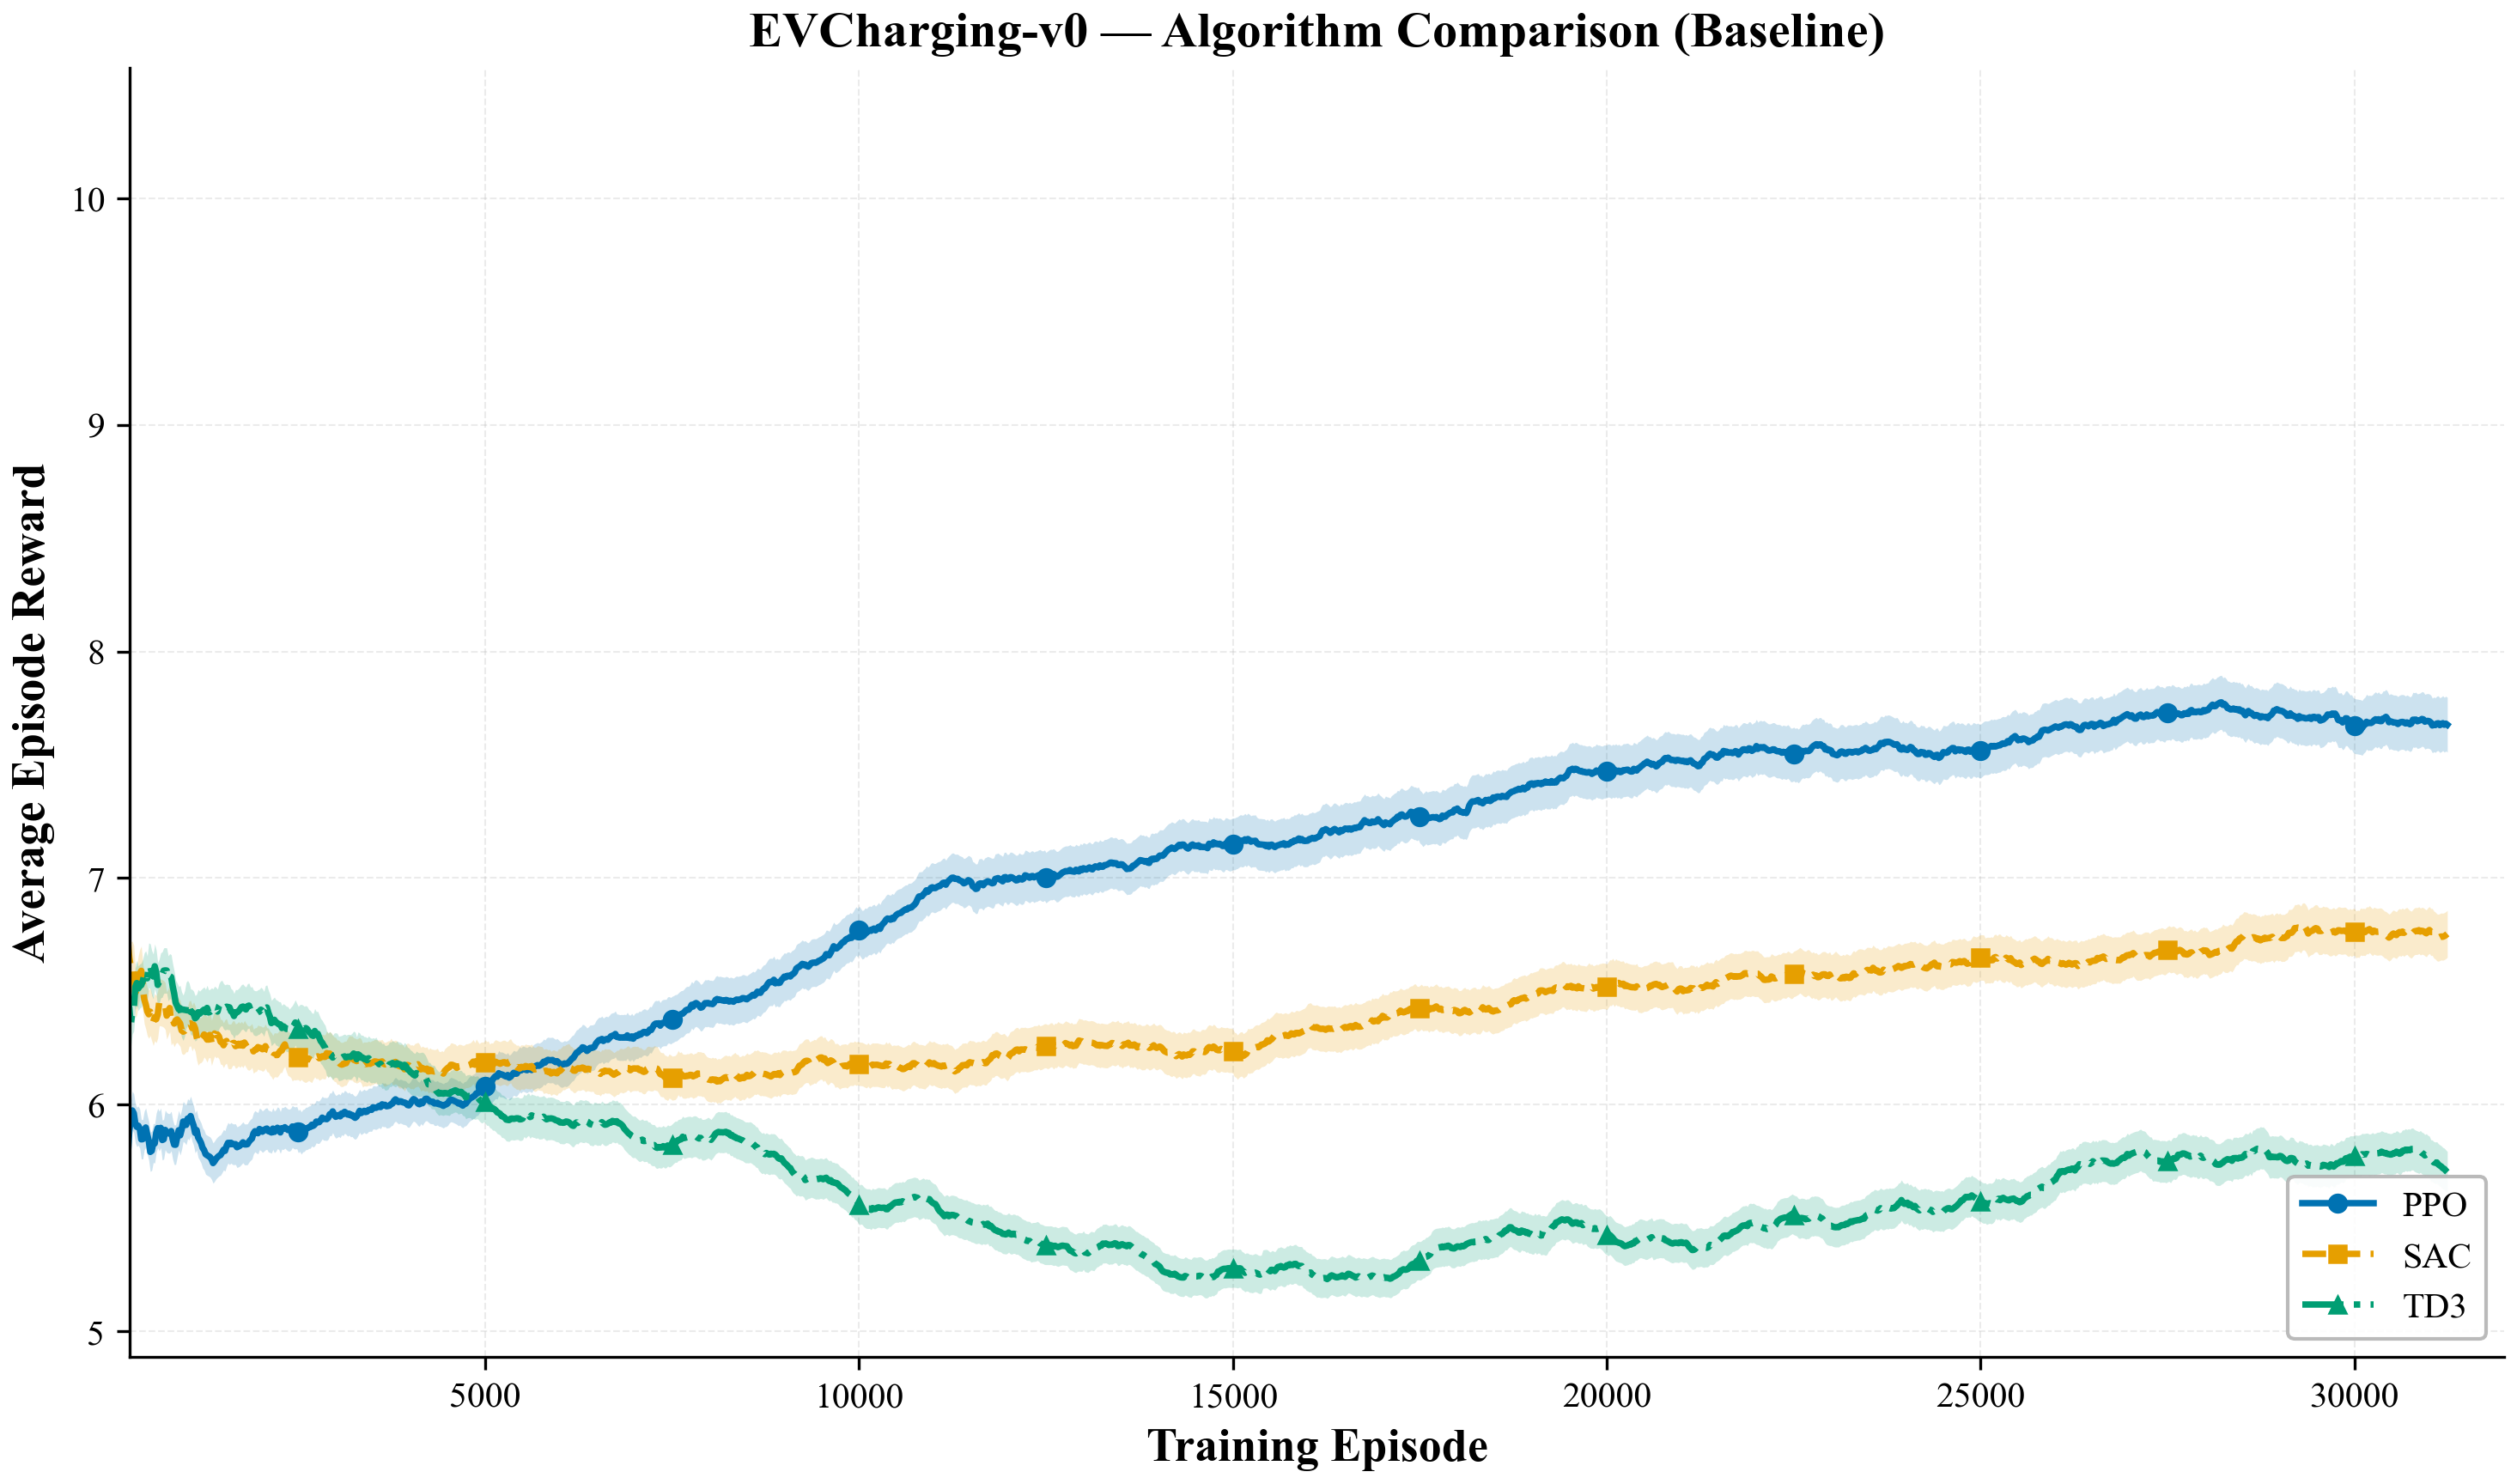
\includegraphics[width=0.9\textwidth]{figures/C_STDRL/ev/comparison/baseline_comparison_2026-03-18_00-03-51.png}
\caption{EV Charging: Baseline training curve comparison across PPO, SAC, and TD3 under clean conditions.}
\label{fig:baseline_ev}
\end{figure}

\begin{figure}[htbp]
\centering
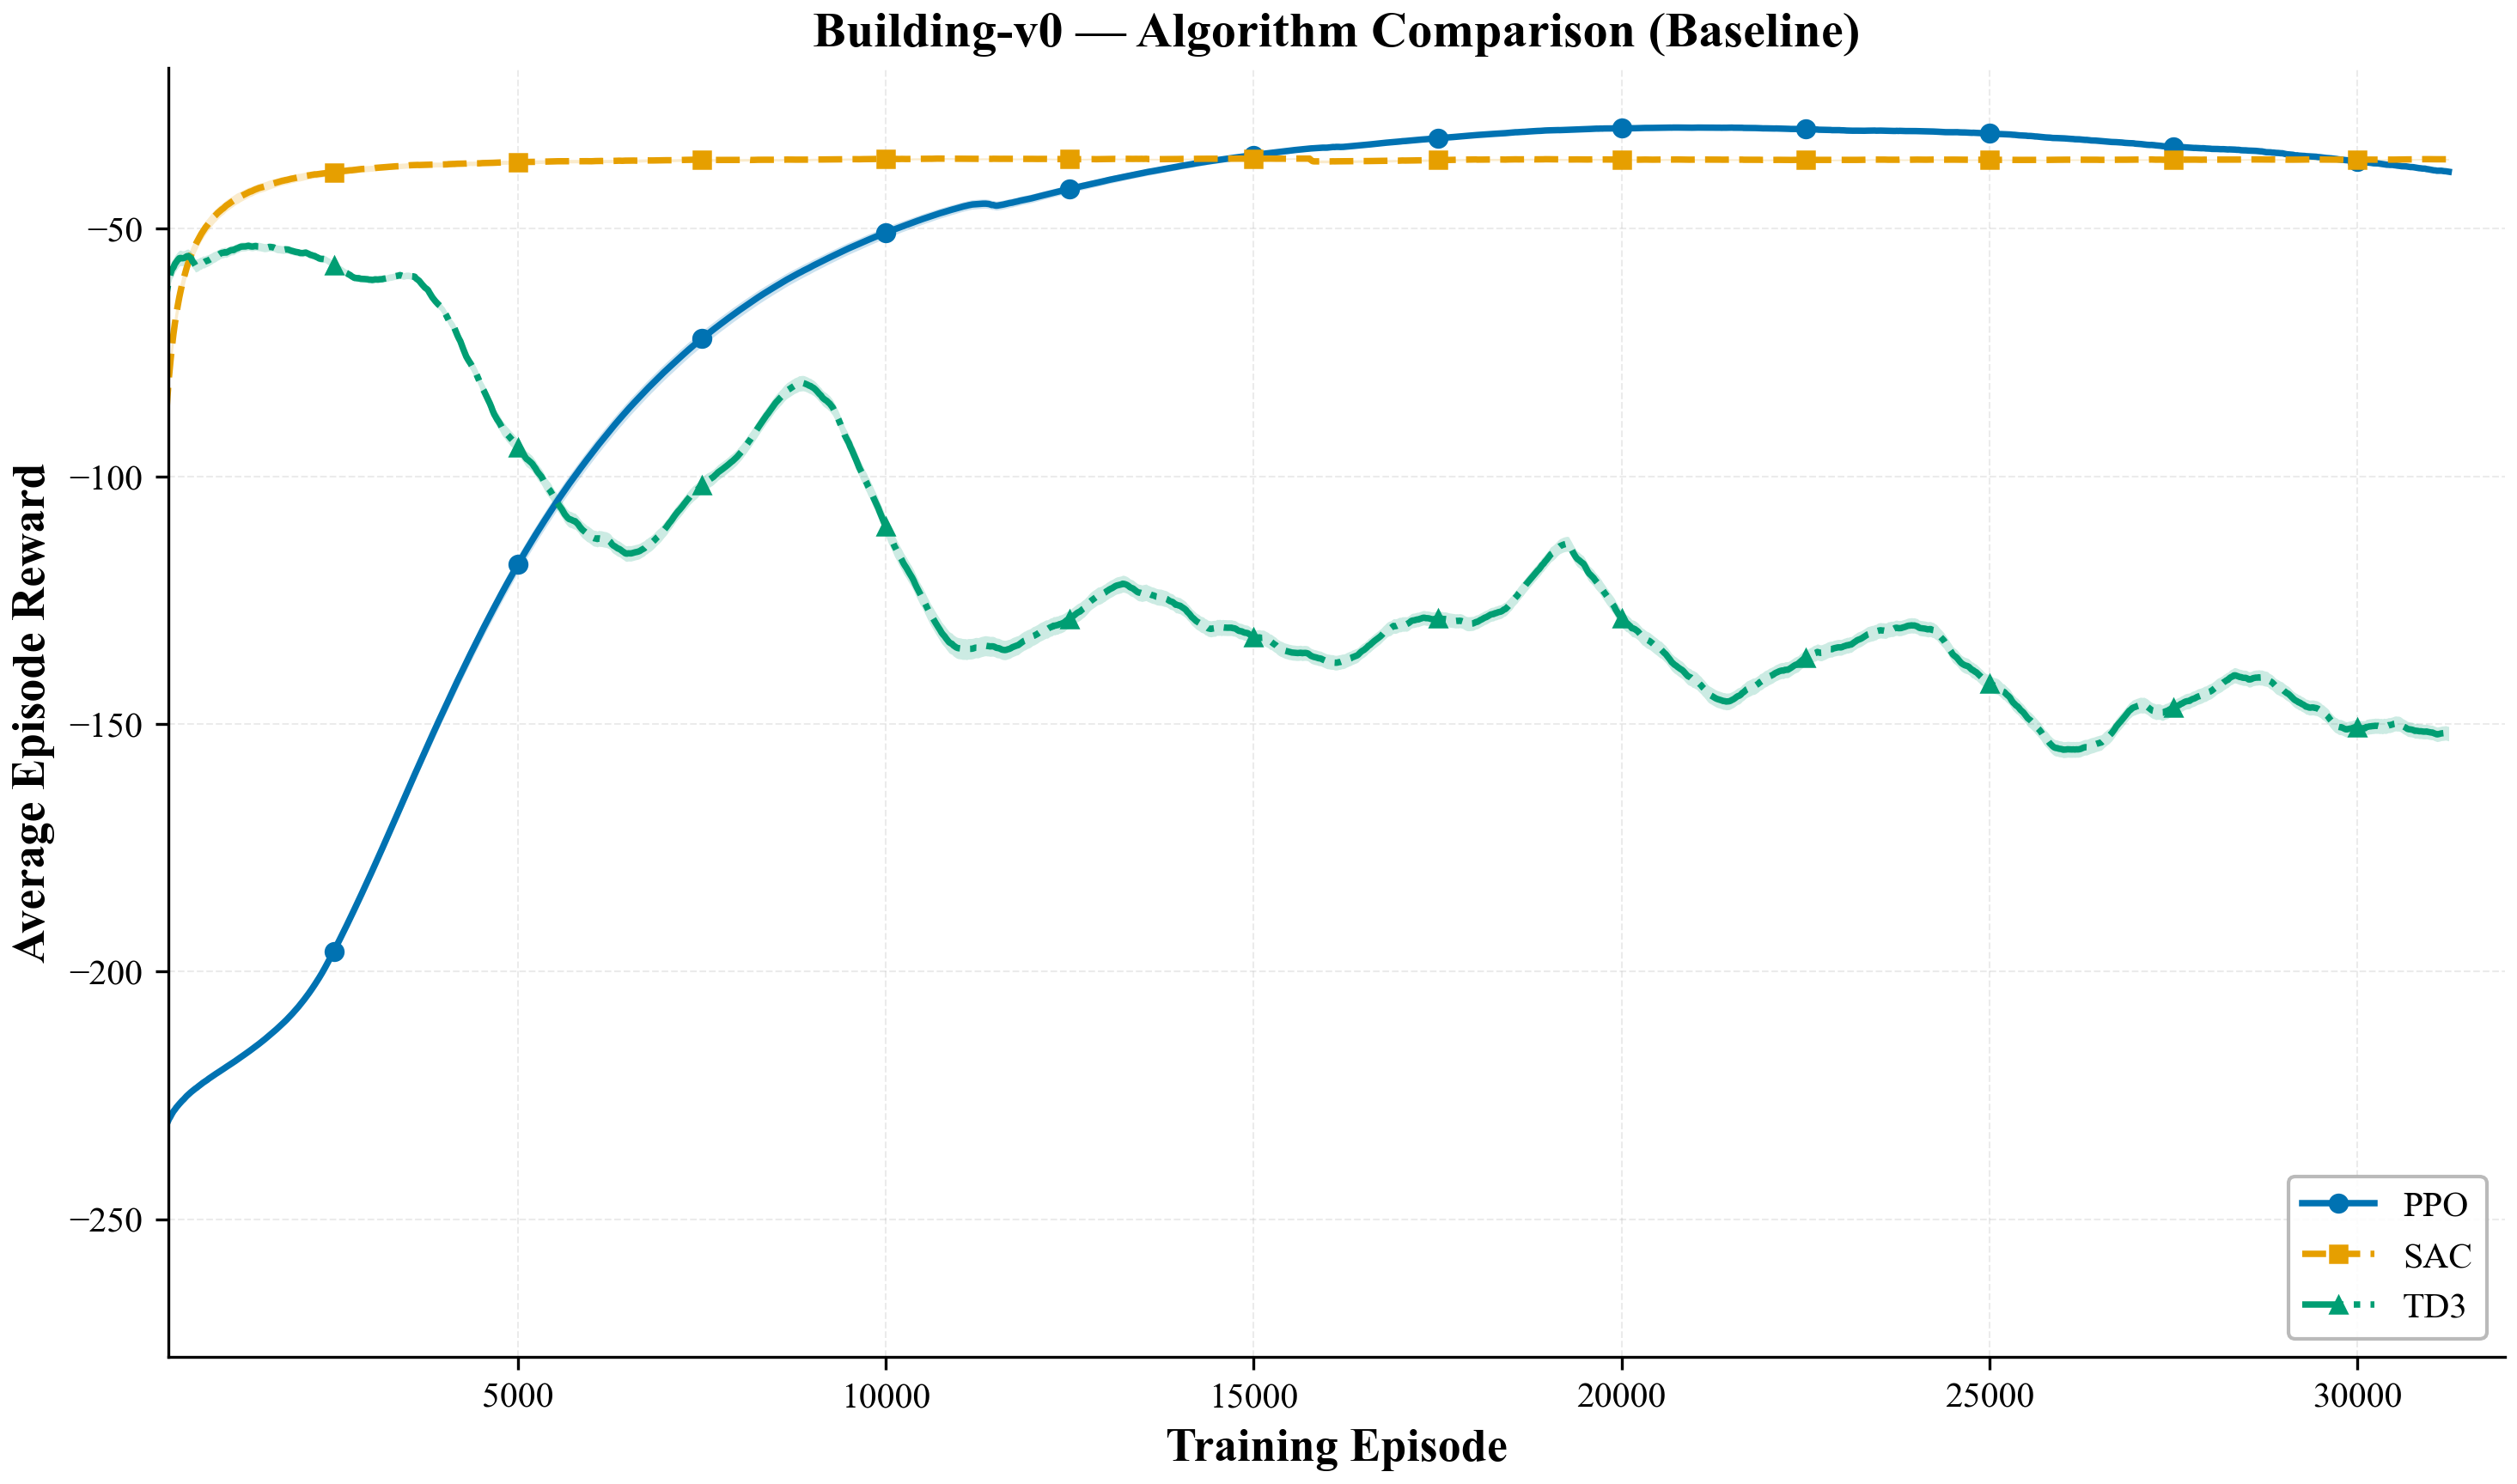
\includegraphics[width=0.9\textwidth]{figures/C_STDRL/bu/comparison/baseline_comparison_2026-03-18_00-04-07.png}
\caption{Building: Baseline training curve comparison across PPO, SAC, and TD3 under clean conditions.}
\label{fig:baseline_bu}
\end{figure}

\begin{figure}[htbp]
\centering
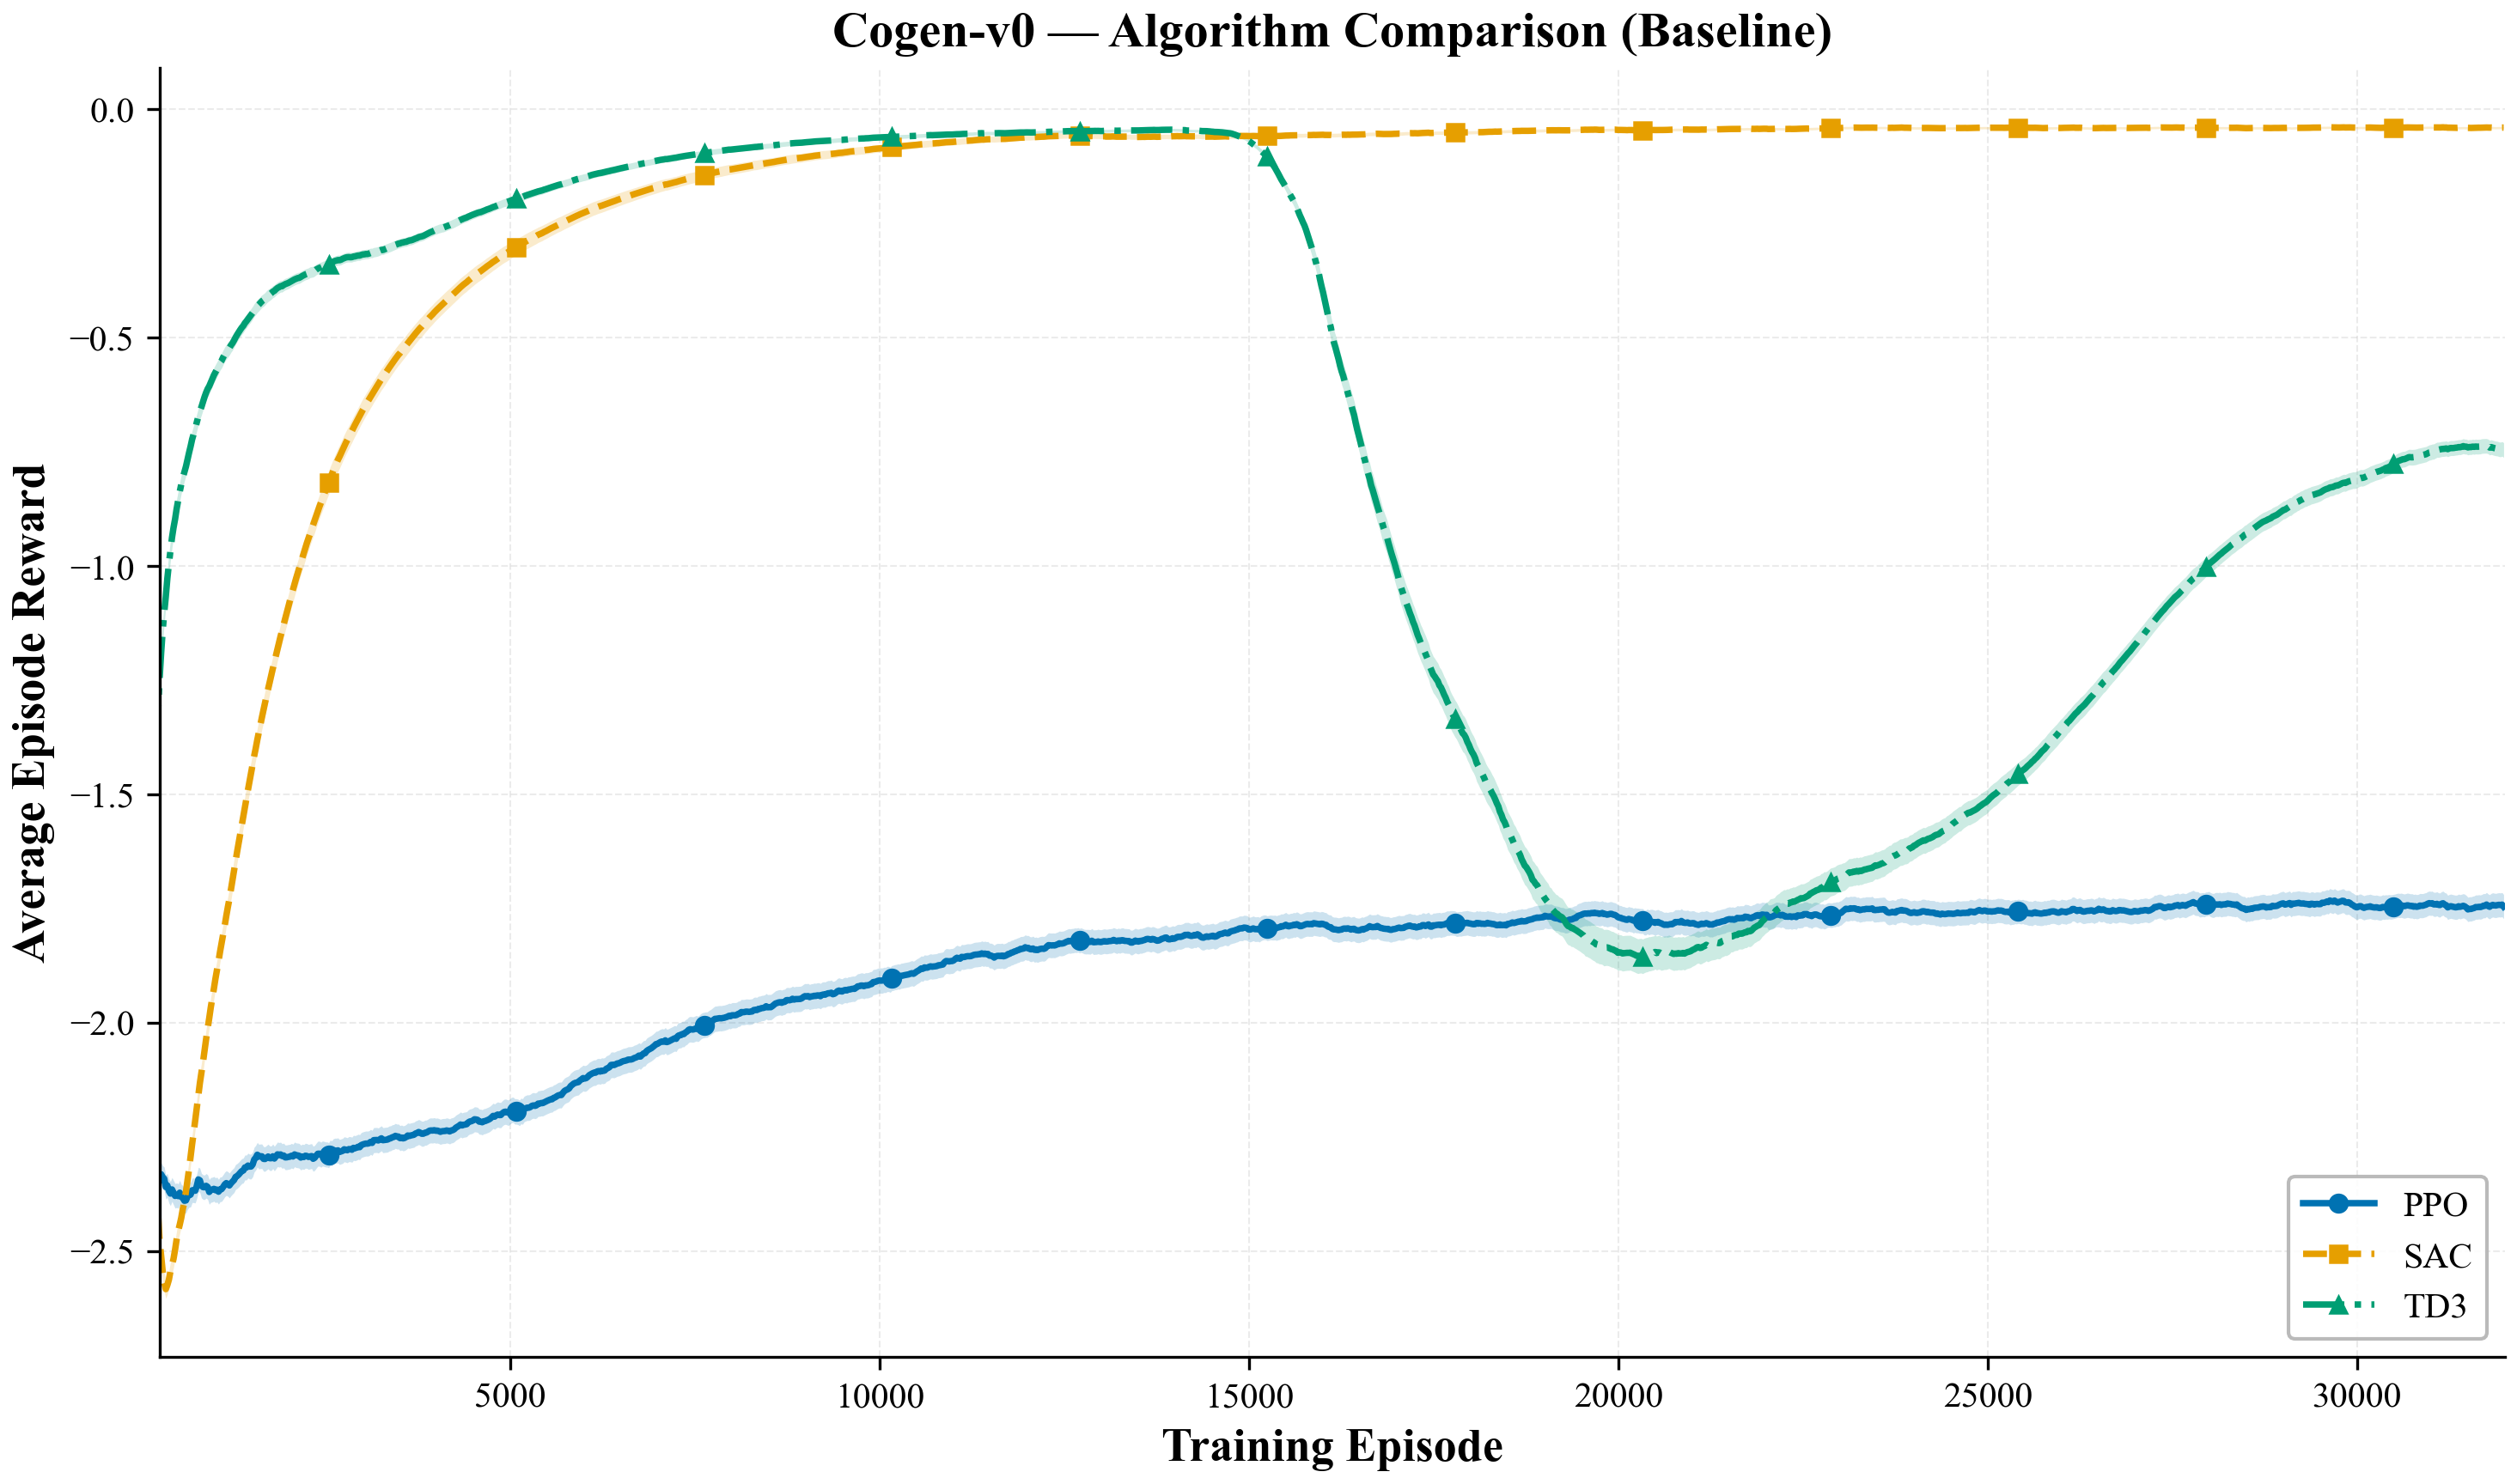
\includegraphics[width=0.9\textwidth]{figures/C_STDRL/co/comparison/baseline_comparison_2026-03-18_00-04-19.png}
\caption{Cogeneration: Baseline training curve comparison across PPO, SAC, and TD3 under clean conditions.}
\label{fig:baseline_co}
\end{figure}

Several environment-specific observations emerge from the baselines:

\paragraph{EV Charging.} PPO significantly outperforms SAC and TD3 in absolute reward ($6.01$ vs.\ $3.79$ and $3.16$), though SAC achieves a slightly higher profit ratio ($0.730$ vs.\ $0.695$). The variance is substantial across all algorithms ($\text{std} \approx 3.1$--$3.5$), reflecting the stochastic nature of EV arrival/departure patterns.

\paragraph{Building.} PPO achieves the best baseline reward ($-32.10$), substantially outperforming TD3 ($-63.20$) and SAC ($-97.71$). The large gap suggests that PPO's on-policy optimization is better suited to the Building environment's multi-zone thermal dynamics. TD3's high variance ($\text{std} = 26.85$) indicates inconsistent HVAC control across episodes.

\paragraph{Cogeneration.} SAC and TD3 achieve near-zero reward ($\approx -0.03$ to $-0.04$), indicating successful plant operation. PPO's reward of $-1.76$ is significantly worse, reflecting PPO's known difficulty with high-dimensional continuous action spaces (15 actuators). However, PPO achieves the lowest fuel cost (\$11,001 vs.\ \$18,700 for SAC), suggesting it learns an overly conservative but fuel-efficient strategy.

% ============================================================
\subsection{EV Charging: Noise Robustness}
\label{sec:noise_ev}

The EV Charging environment exhibits remarkable robustness to all noise types across all algorithms. This resilience stems from the environment's reward structure, which depends primarily on aggregate daily charging patterns rather than instantaneous observations.

% --- EV PPO ---
\subsubsection{EV Charging --- PPO}

\paragraph{Training curves.} \Cref{fig:stdrl_ev_ppo_ds,fig:stdrl_ev_ppo_da,fig:stdrl_ev_ppo_de} show PPO training curves under observation, action, and environment noise respectively. Convergence is virtually unaffected across all noise levels, with final rewards clustering tightly around the clean baseline.

\begin{figure}[htbp]
\centering
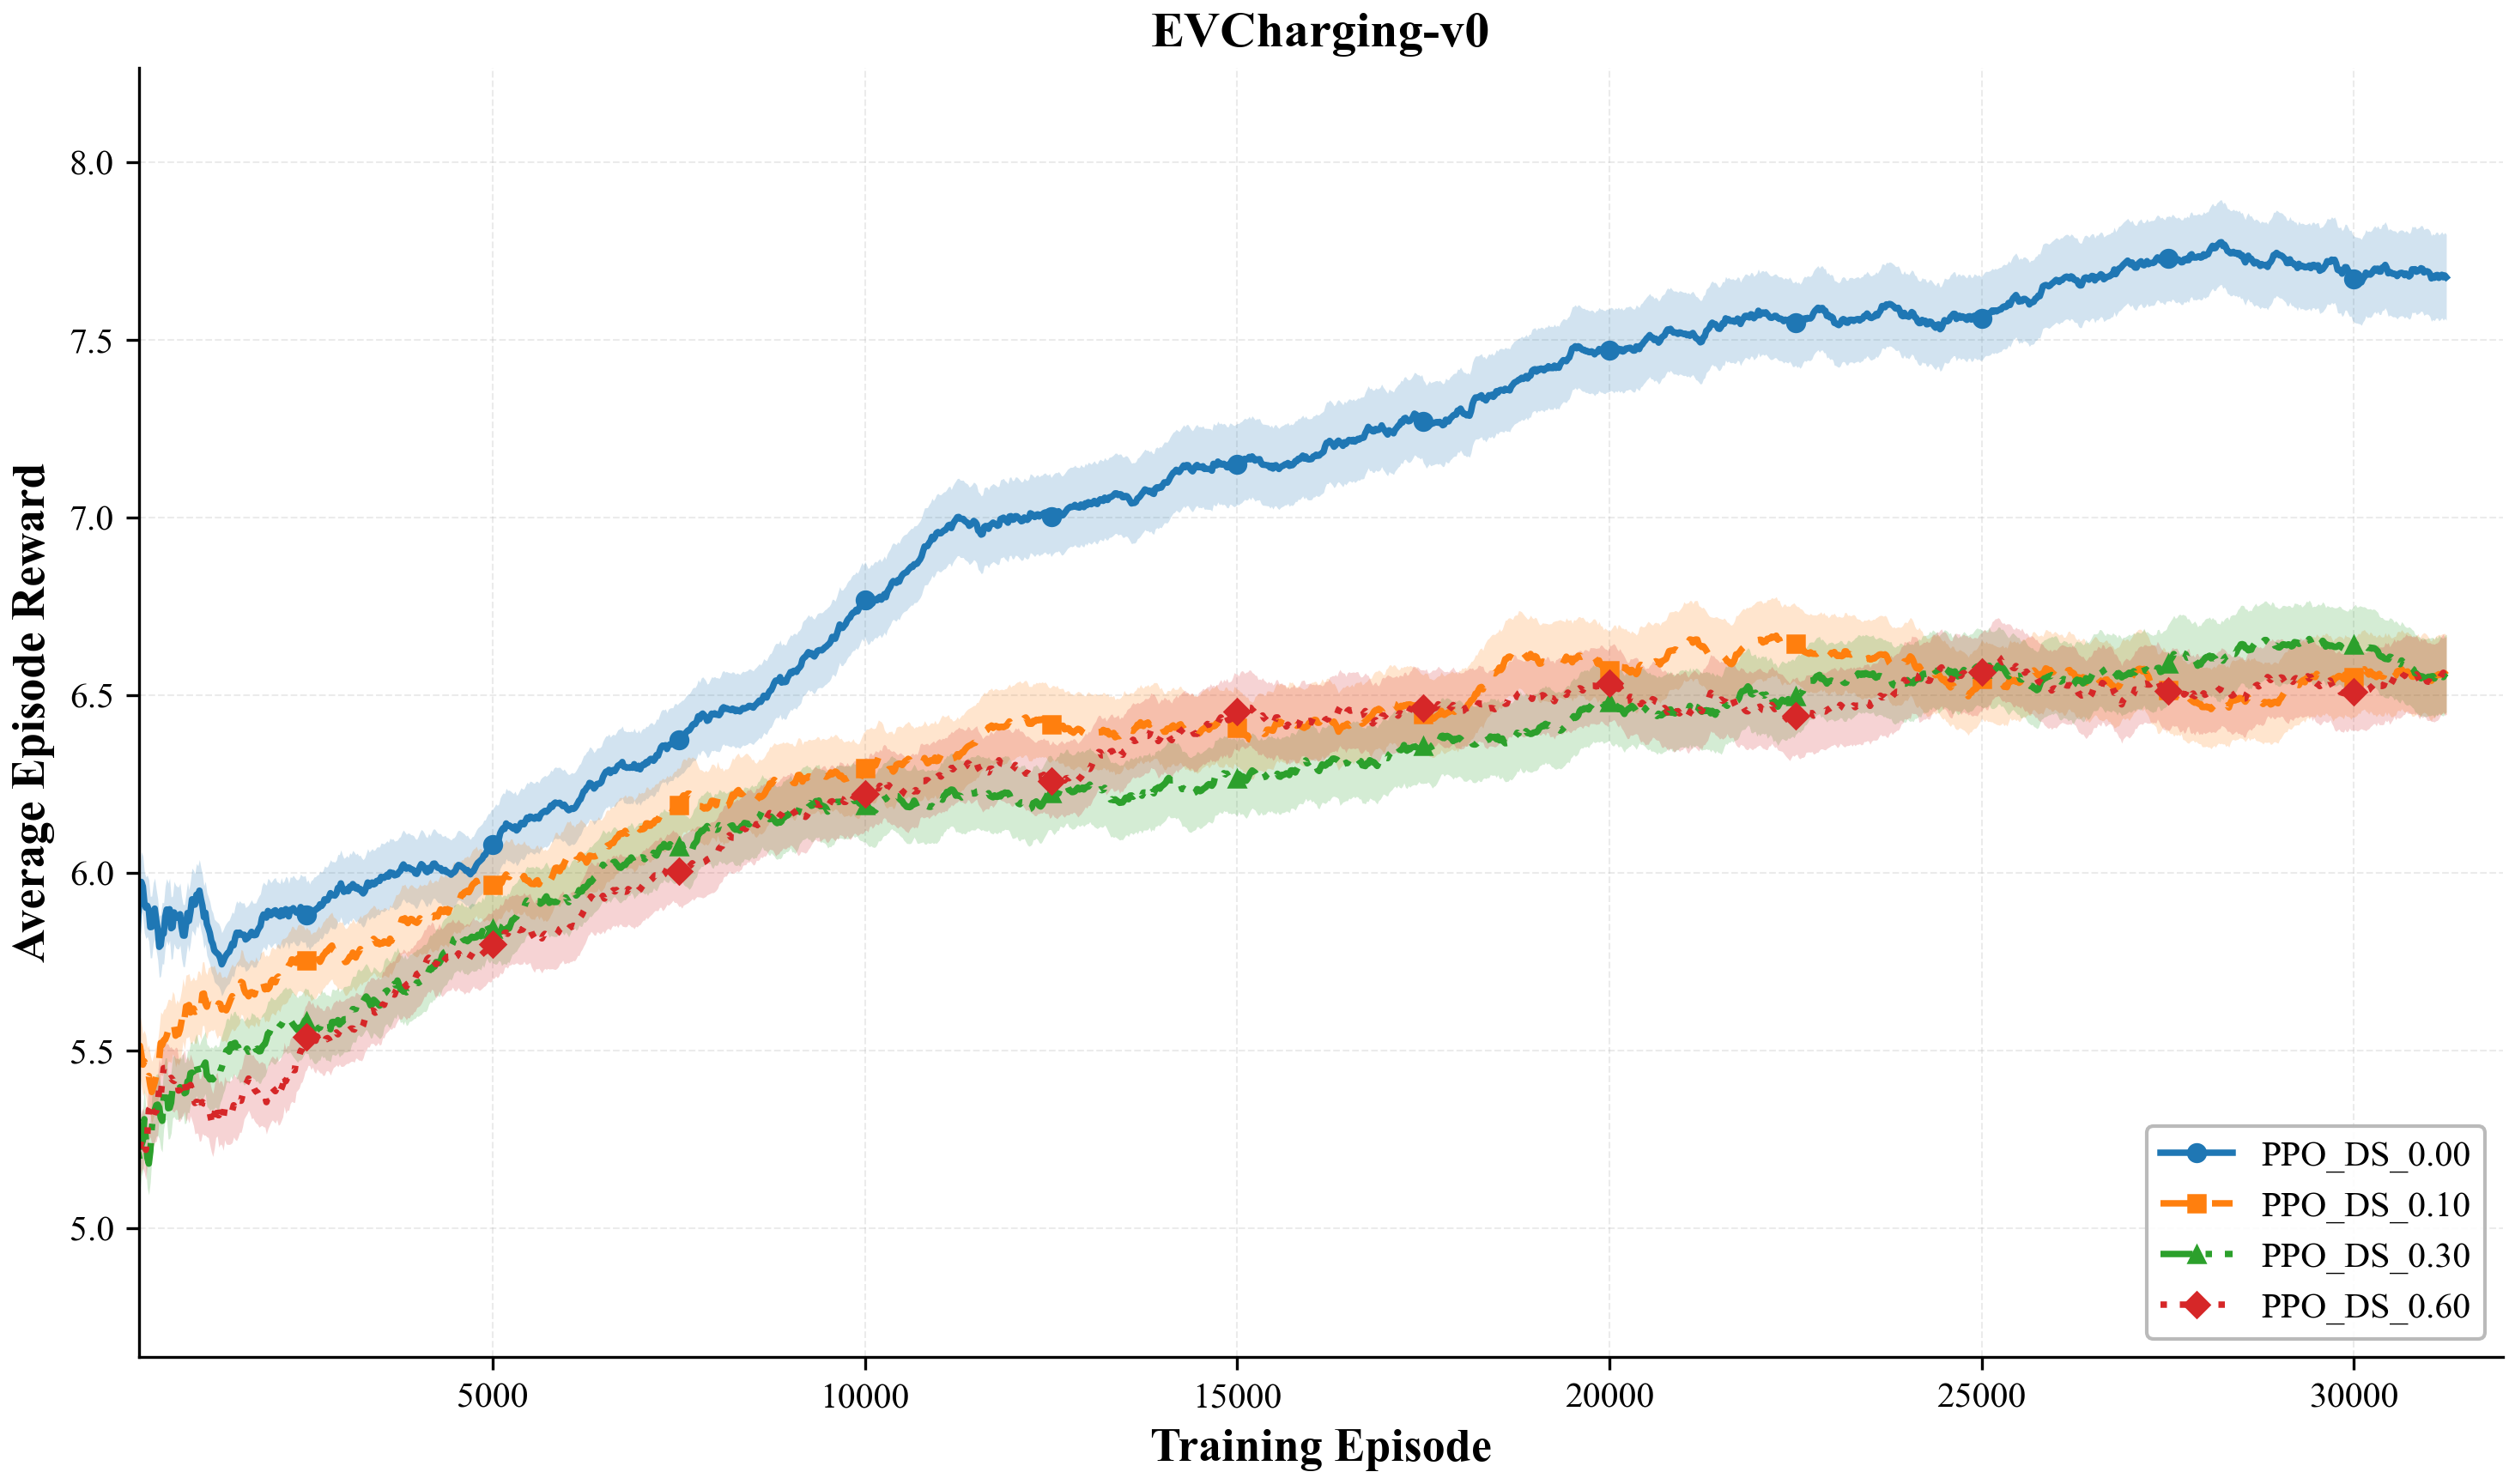
\includegraphics[width=0.9\textwidth]{figures/C_STDRL/ev/PPO/DS_2026-03-16_23-32-01.png}
\caption{EV Charging PPO: Training curves under observation noise (DS) at varying intensities.}
\label{fig:stdrl_ev_ppo_ds}
\end{figure}

\begin{figure}[htbp]
\centering
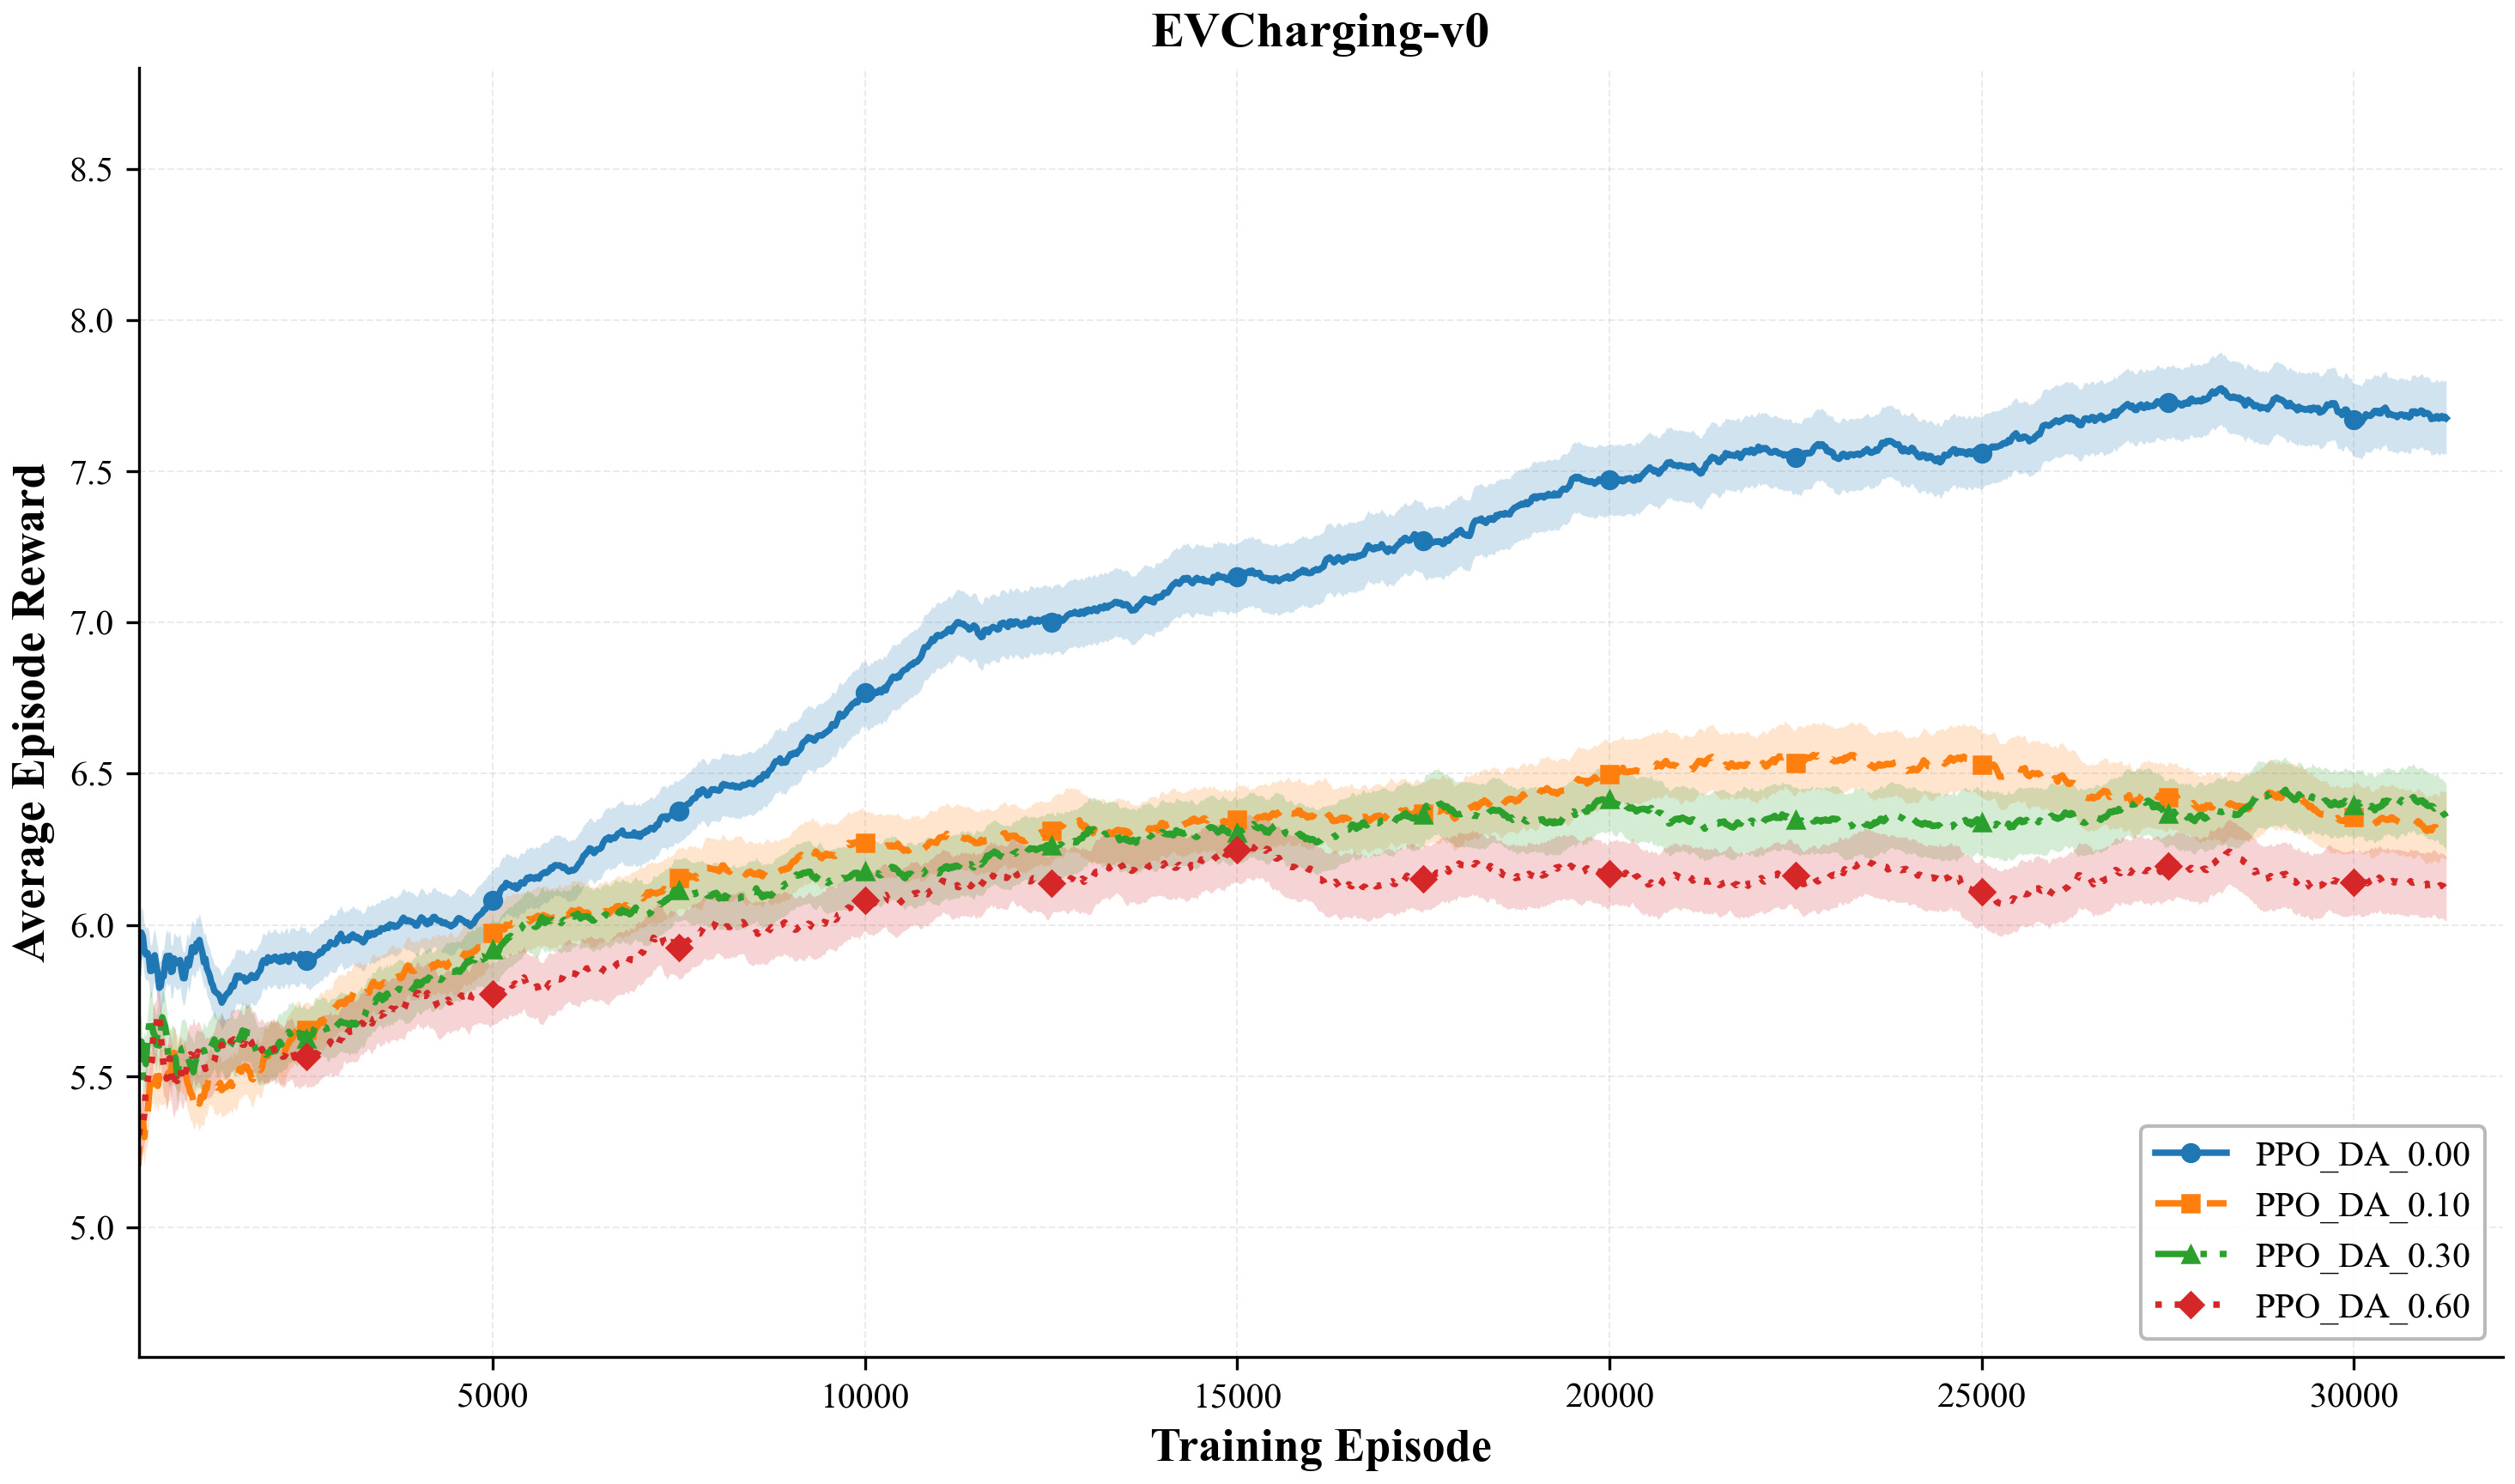
\includegraphics[width=0.9\textwidth]{figures/C_STDRL/ev/PPO/DA_2026-03-16_23-32-03.png}
\caption{EV Charging PPO: Training curves under action noise (DA) at varying intensities.}
\label{fig:stdrl_ev_ppo_da}
\end{figure}

\begin{figure}[htbp]
\centering
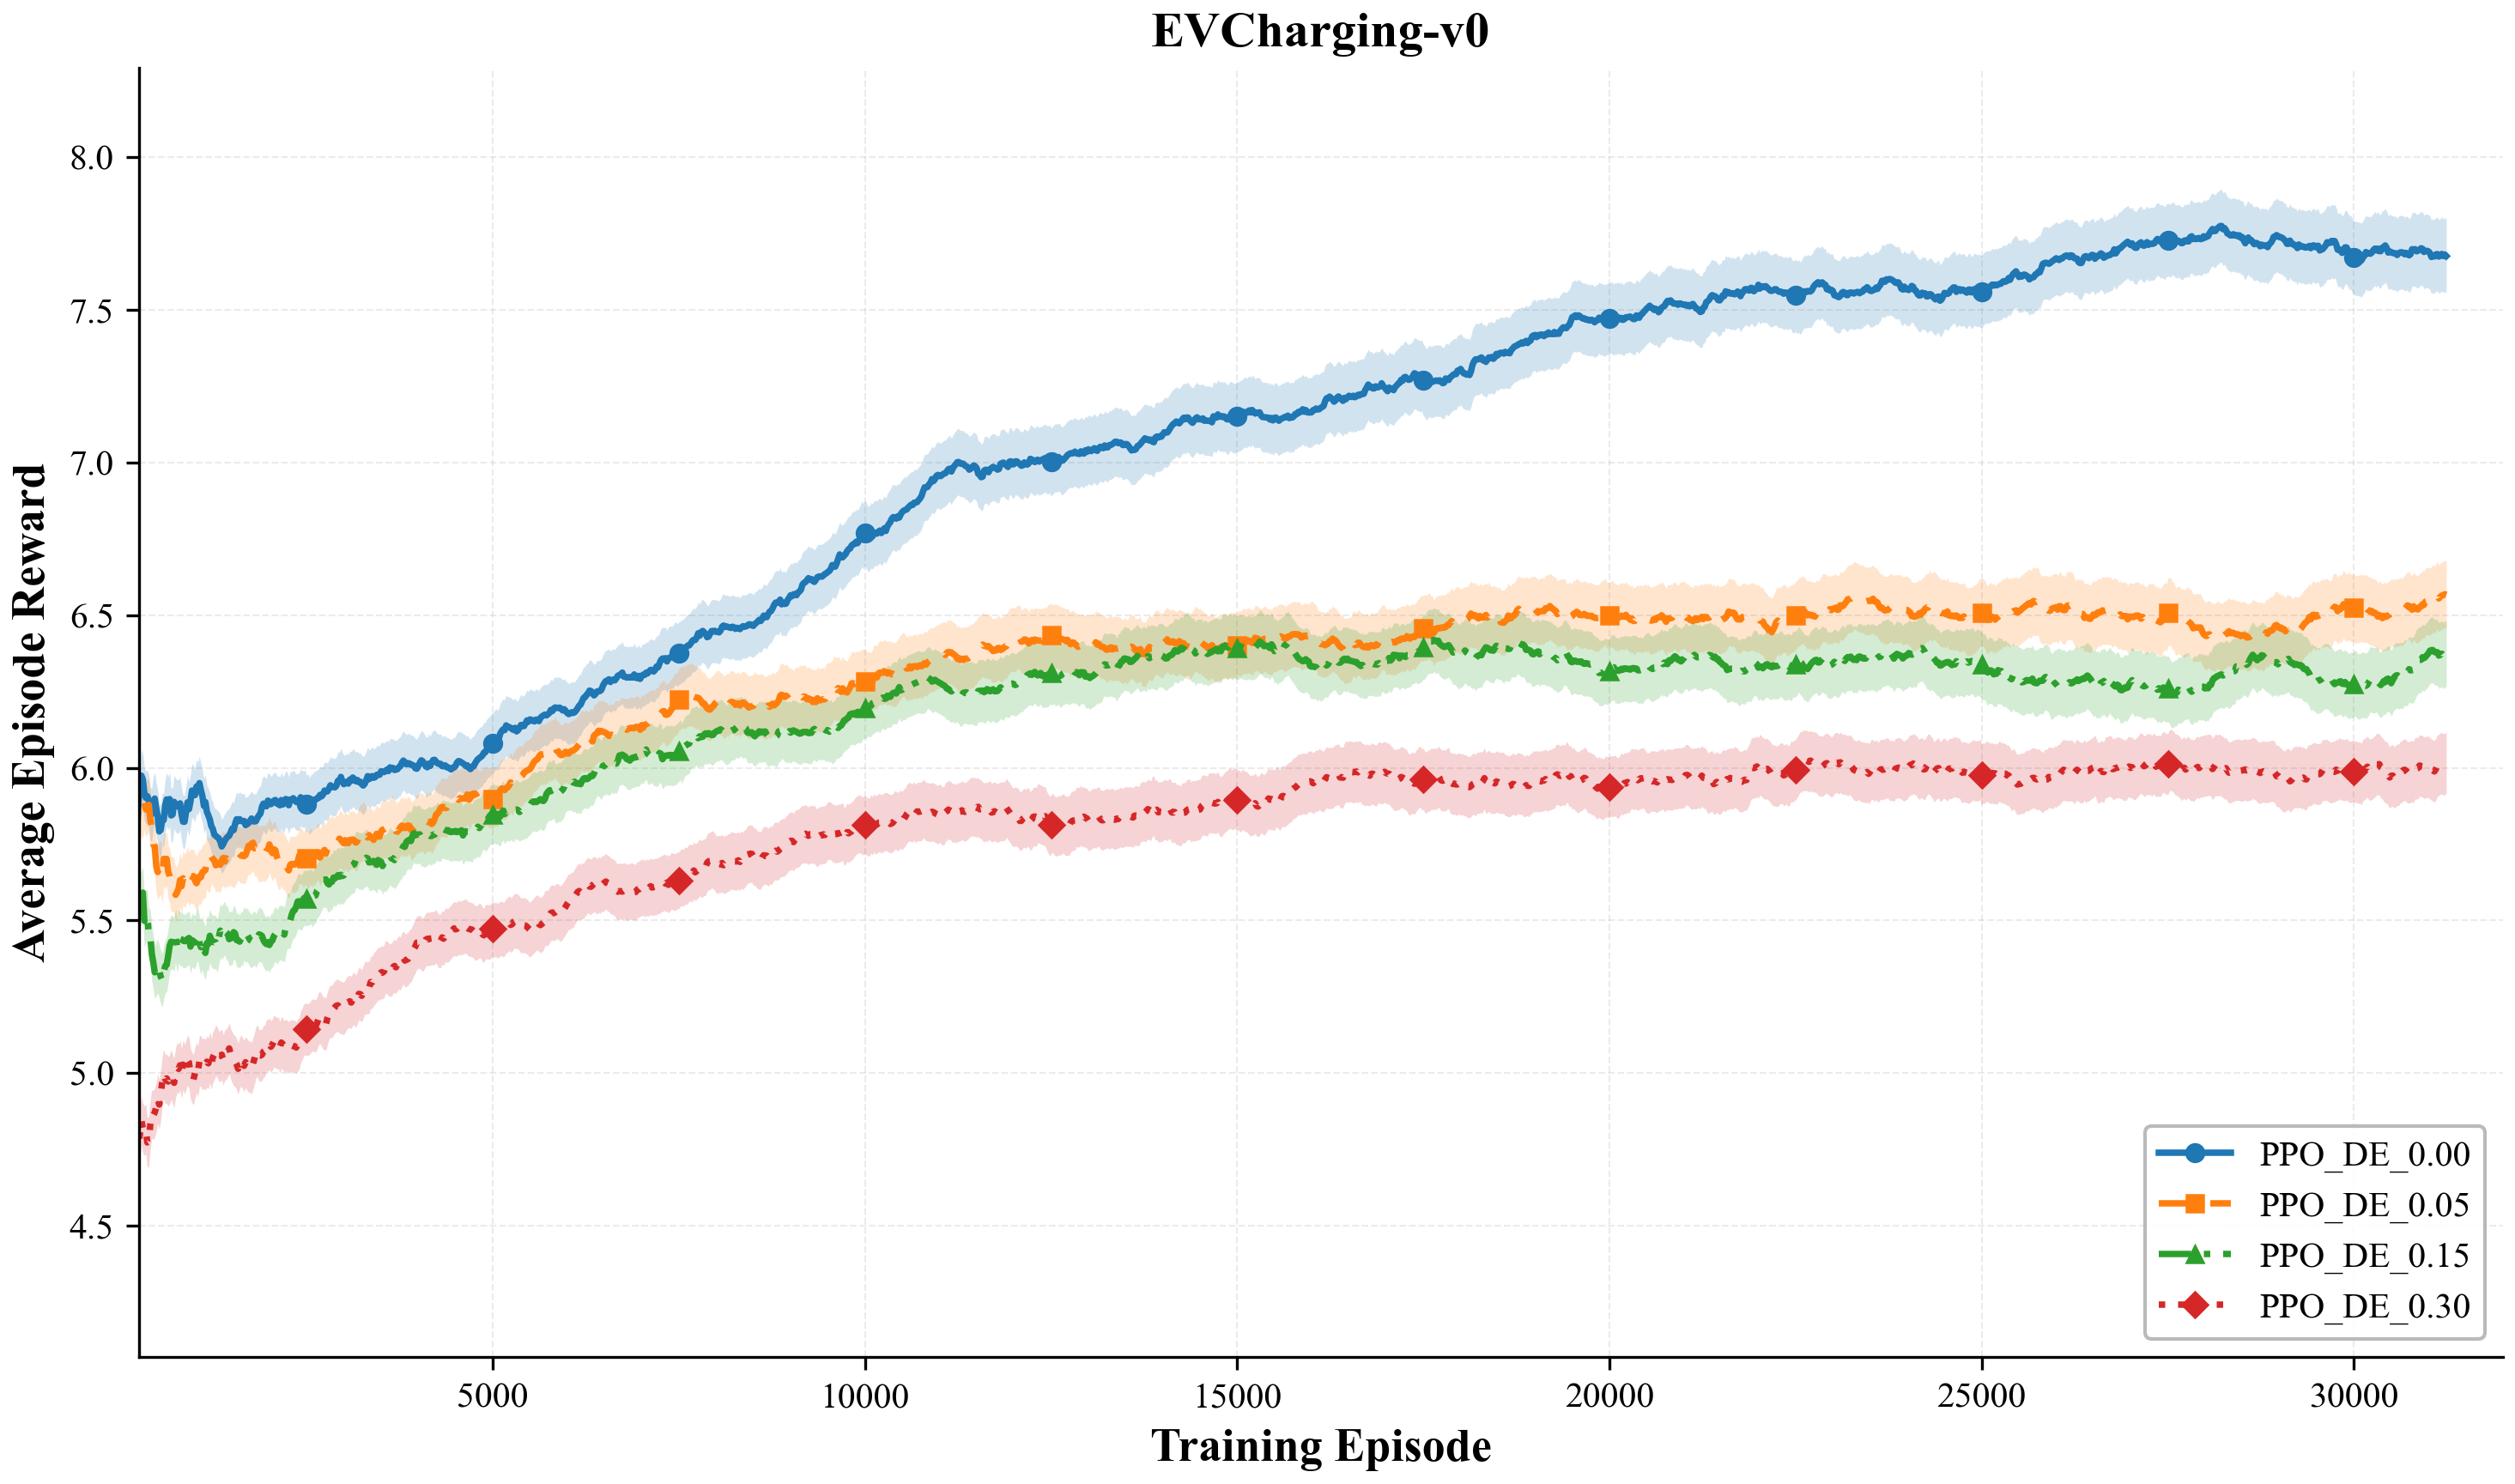
\includegraphics[width=0.9\textwidth]{figures/C_STDRL/ev/PPO/DE_2026-03-16_23-32-04.png}
\caption{EV Charging PPO: Training curves under environment noise (DE) at varying intensities.}
\label{fig:stdrl_ev_ppo_de}
\end{figure}

\paragraph{Test-time robustness.} The violin plots in \Cref{fig:violin_ev_ppo_obs,fig:violin_ev_ppo_act,fig:violin_ev_ppo_env} confirm that the reward distribution remains stable across all noise channels. The distributional shape is virtually unchanged even at extreme noise levels, with no shift in the mode or emergence of heavy tails.

\begin{figure}[htbp]
\centering

\includegraphics[width=0.9\textwidth]{figures/C_POST/evcharging/PPO/obs_violin.png}
\caption{EV Charging PPO: Reward distribution under observation noise. The distribution remains stable across noise levels, confirming exceptional robustness to sensor uncertainty.}
\label{fig:violin_ev_ppo_obs}
\end{figure}

\begin{figure}[htbp]
\centering

\includegraphics[width=0.9\textwidth]{figures/C_POST/evcharging/PPO/action_violin.png}
\caption{EV Charging PPO: Reward distribution under action noise.}
\label{fig:violin_ev_ppo_act}
\end{figure}

\begin{figure}[htbp]
\centering

\includegraphics[width=0.9\textwidth]{figures/C_POST/evcharging/PPO/env_violin.png}
\caption{EV Charging PPO: Reward distribution under environment noise.}
\label{fig:violin_ev_ppo_env}
\end{figure}

\begin{figure}[htbp]
\centering

\includegraphics[width=0.9\textwidth]{figures/C_POST/evcharging/PPO/panel.png}
\caption{EV Charging PPO: Summary panel across all three noise channels. Mean reward degradation is negligible ($<1\%$) across the full noise range.}
\label{fig:post_ev_ppo_panel}
\end{figure}

% --- EV SAC ---
\subsubsection{EV Charging --- SAC}

\paragraph{Training curves.} \Cref{fig:stdrl_ev_sac_ds,fig:stdrl_ev_sac_da,fig:stdrl_ev_sac_de} show SAC training curves under all noise types.

\begin{figure}[htbp]
\centering
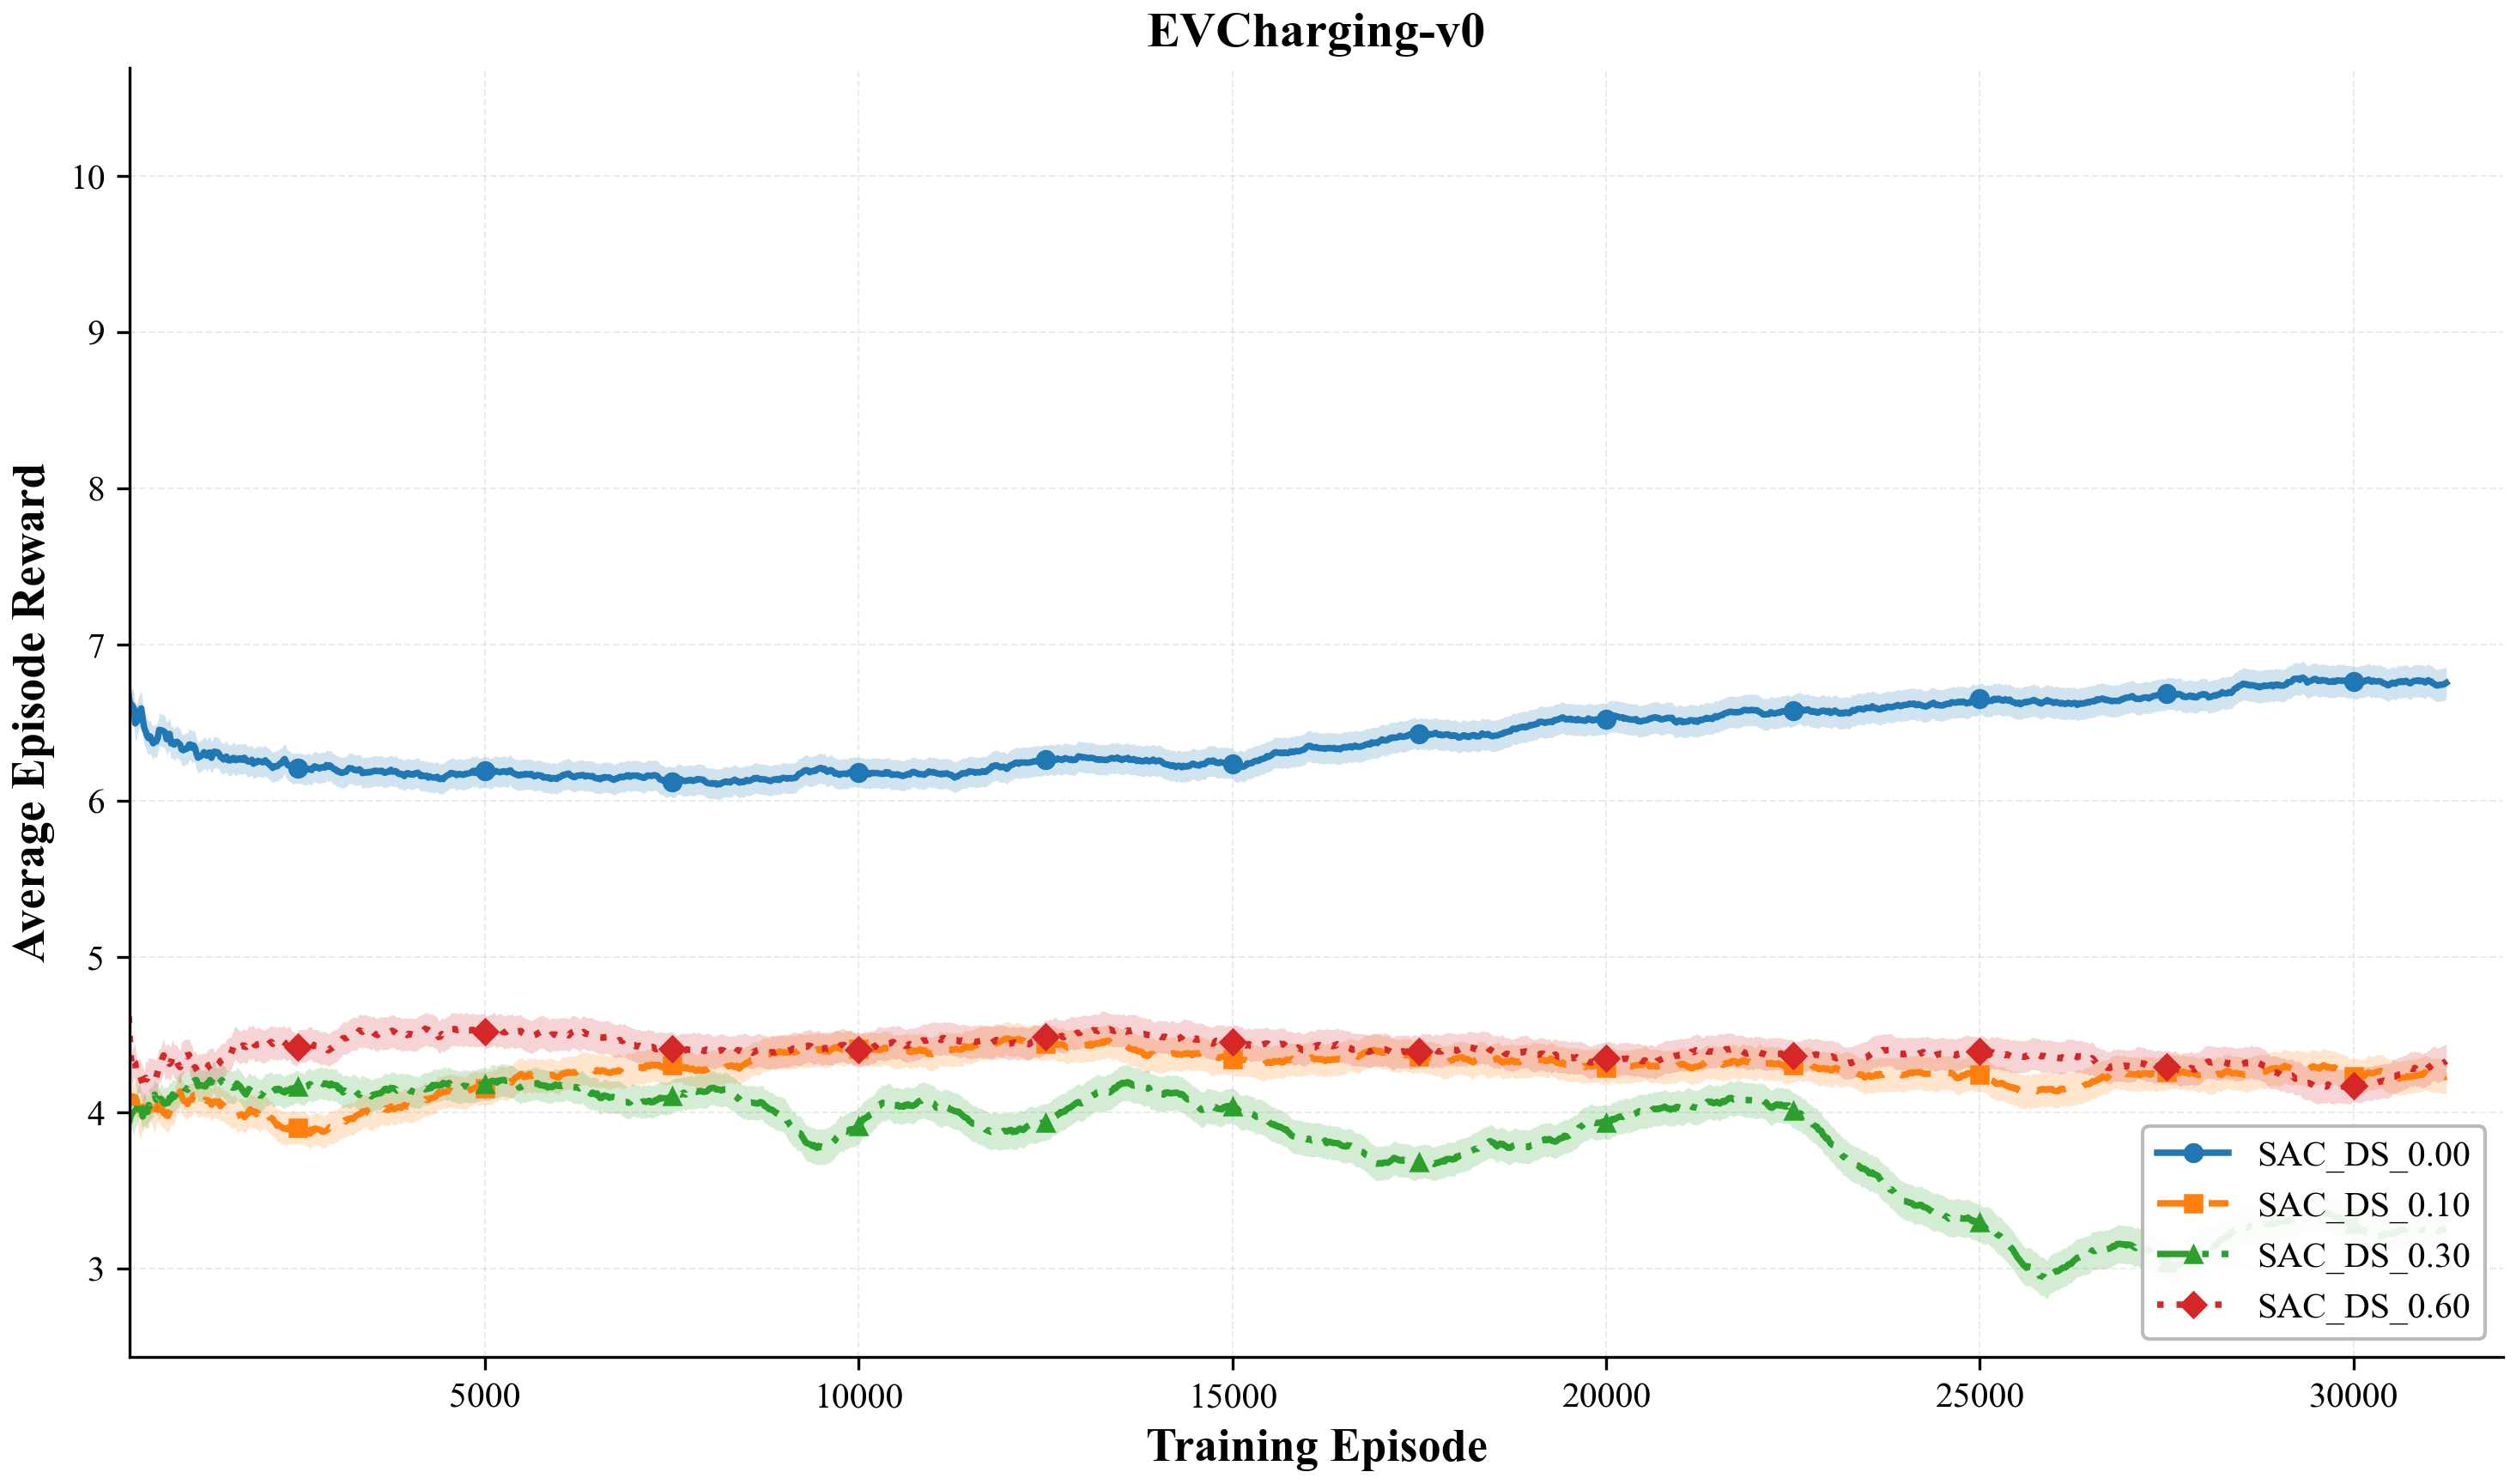
\includegraphics[width=0.9\textwidth]{figures/C_STDRL/ev/SAC/DS_2026-03-16_23-32-06.png}
\caption{EV Charging SAC: Training curves under observation noise (DS).}
\label{fig:stdrl_ev_sac_ds}
\end{figure}

\begin{figure}[htbp]
\centering
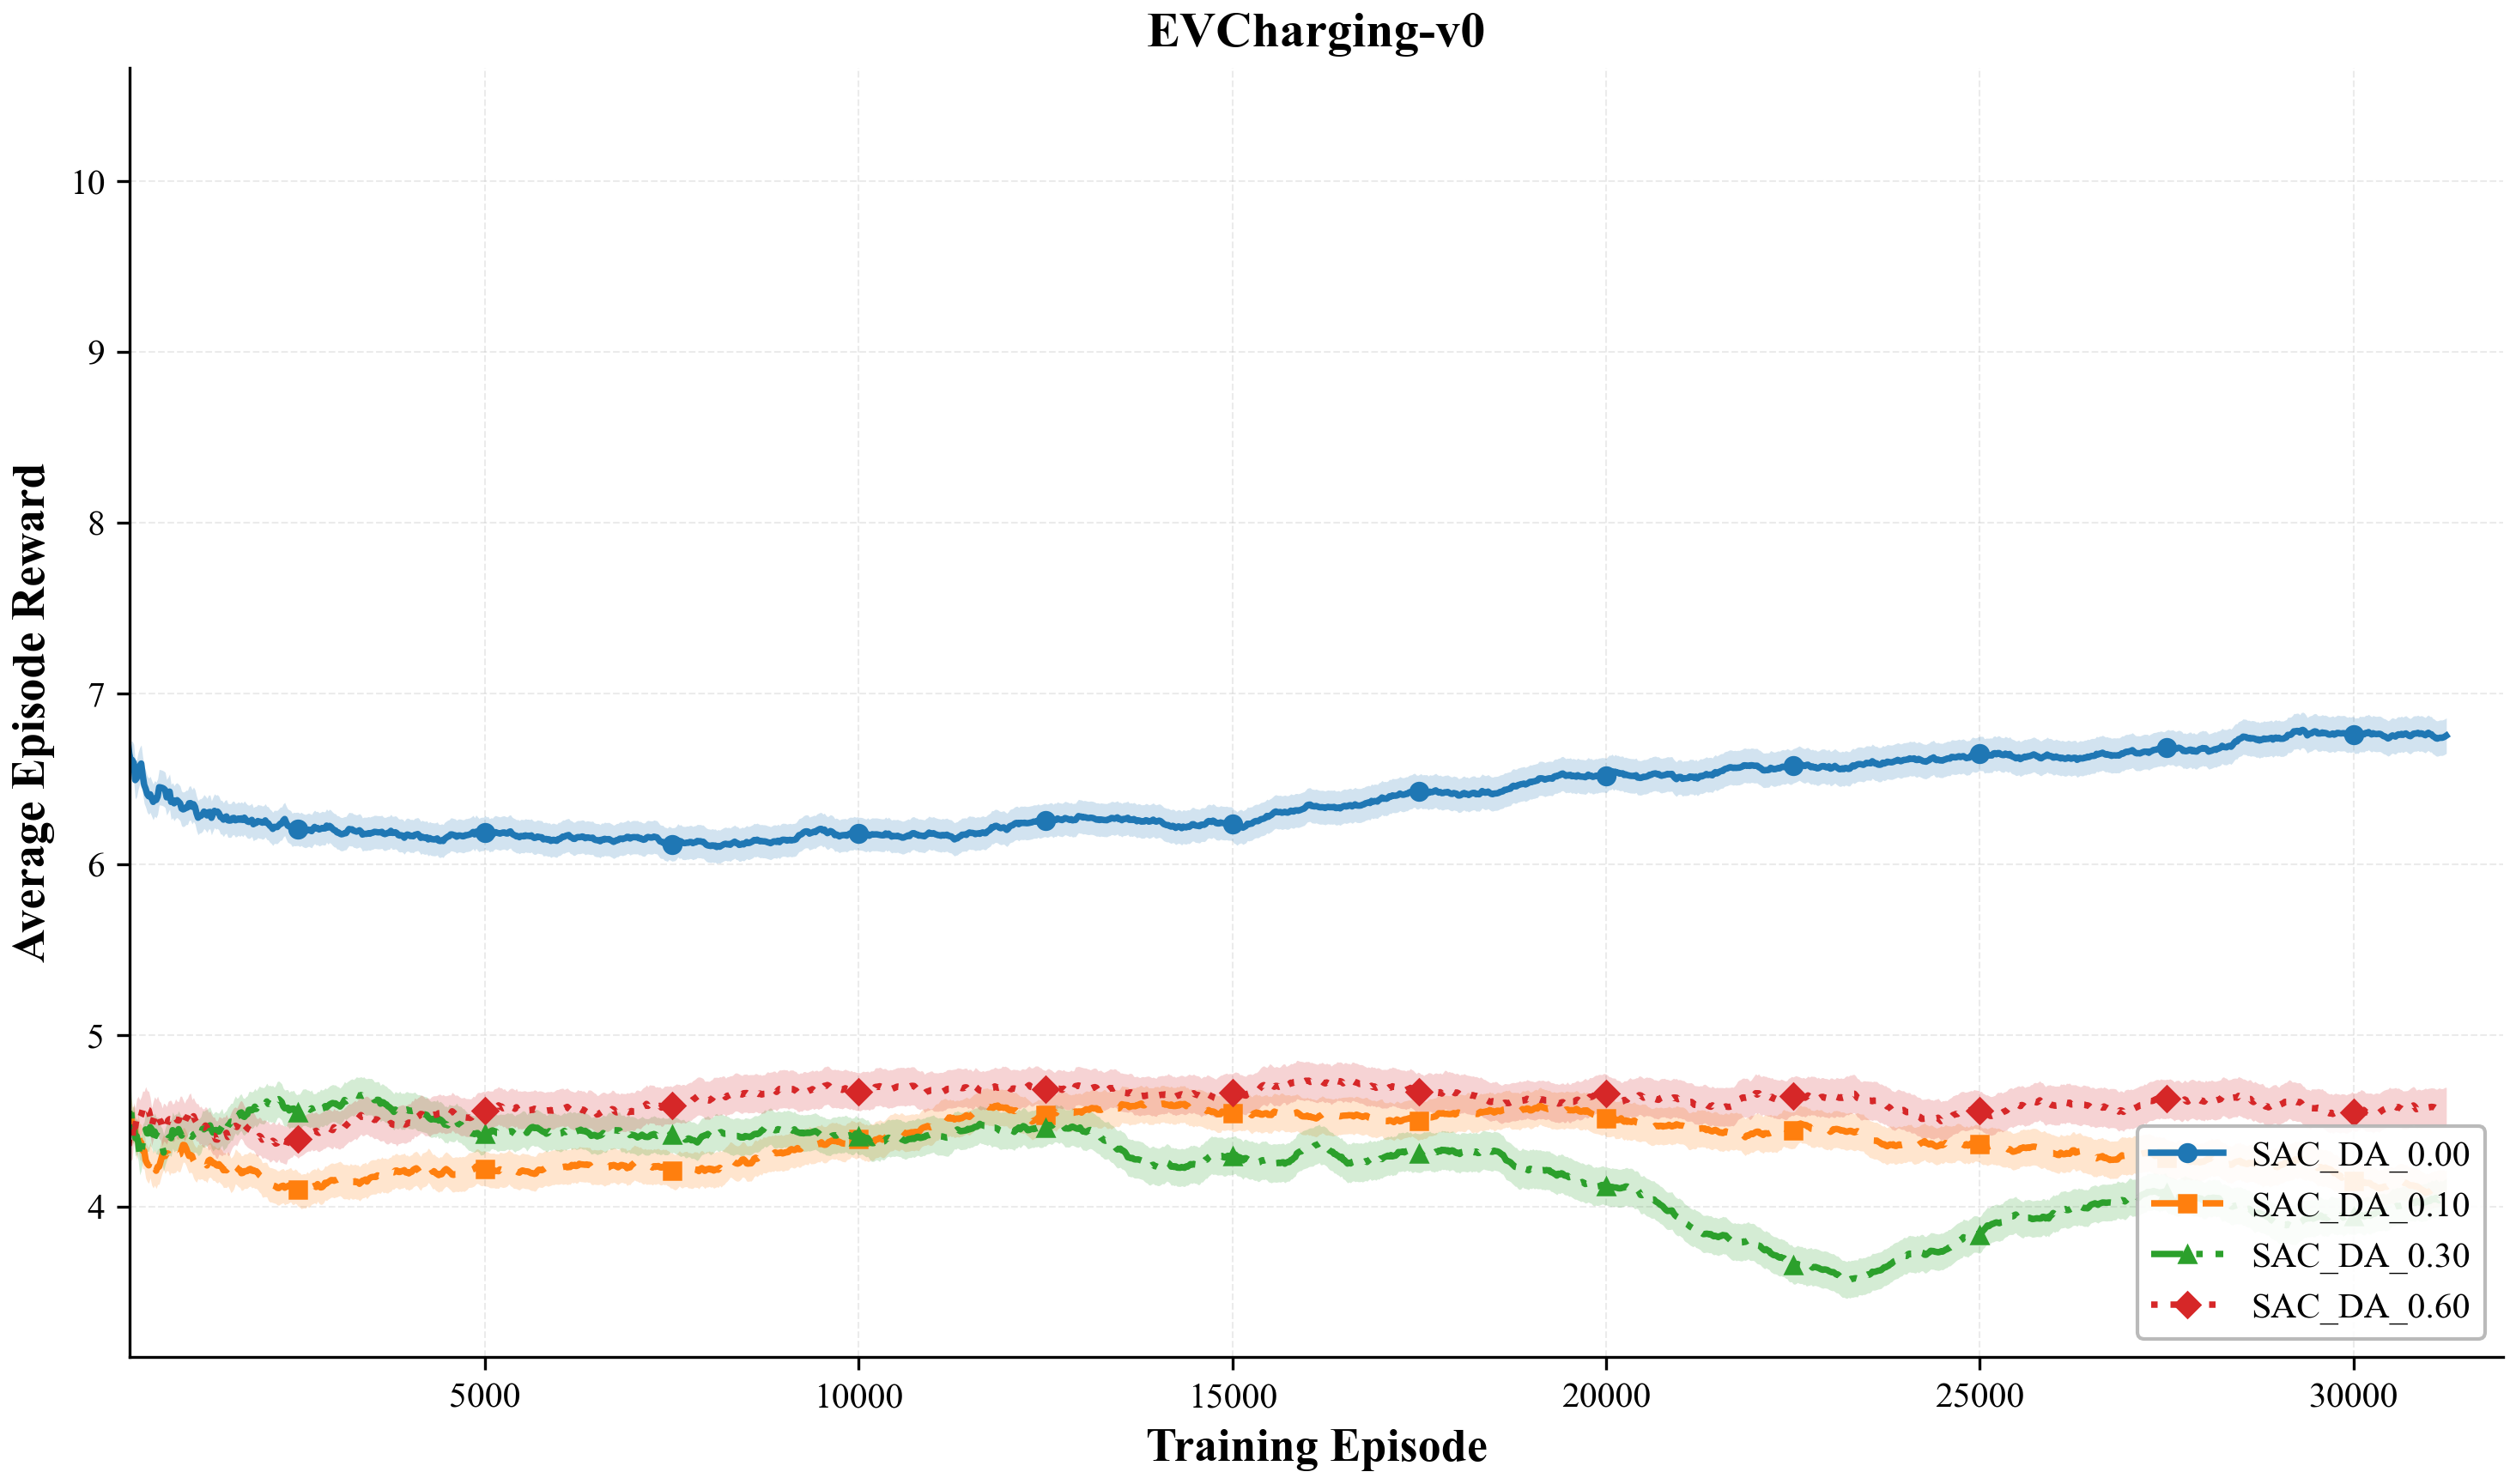
\includegraphics[width=0.9\textwidth]{figures/C_STDRL/ev/SAC/DA_2026-03-16_23-32-09.png}
\caption{EV Charging SAC: Training curves under action noise (DA).}
\label{fig:stdrl_ev_sac_da}
\end{figure}

\begin{figure}[htbp]
\centering
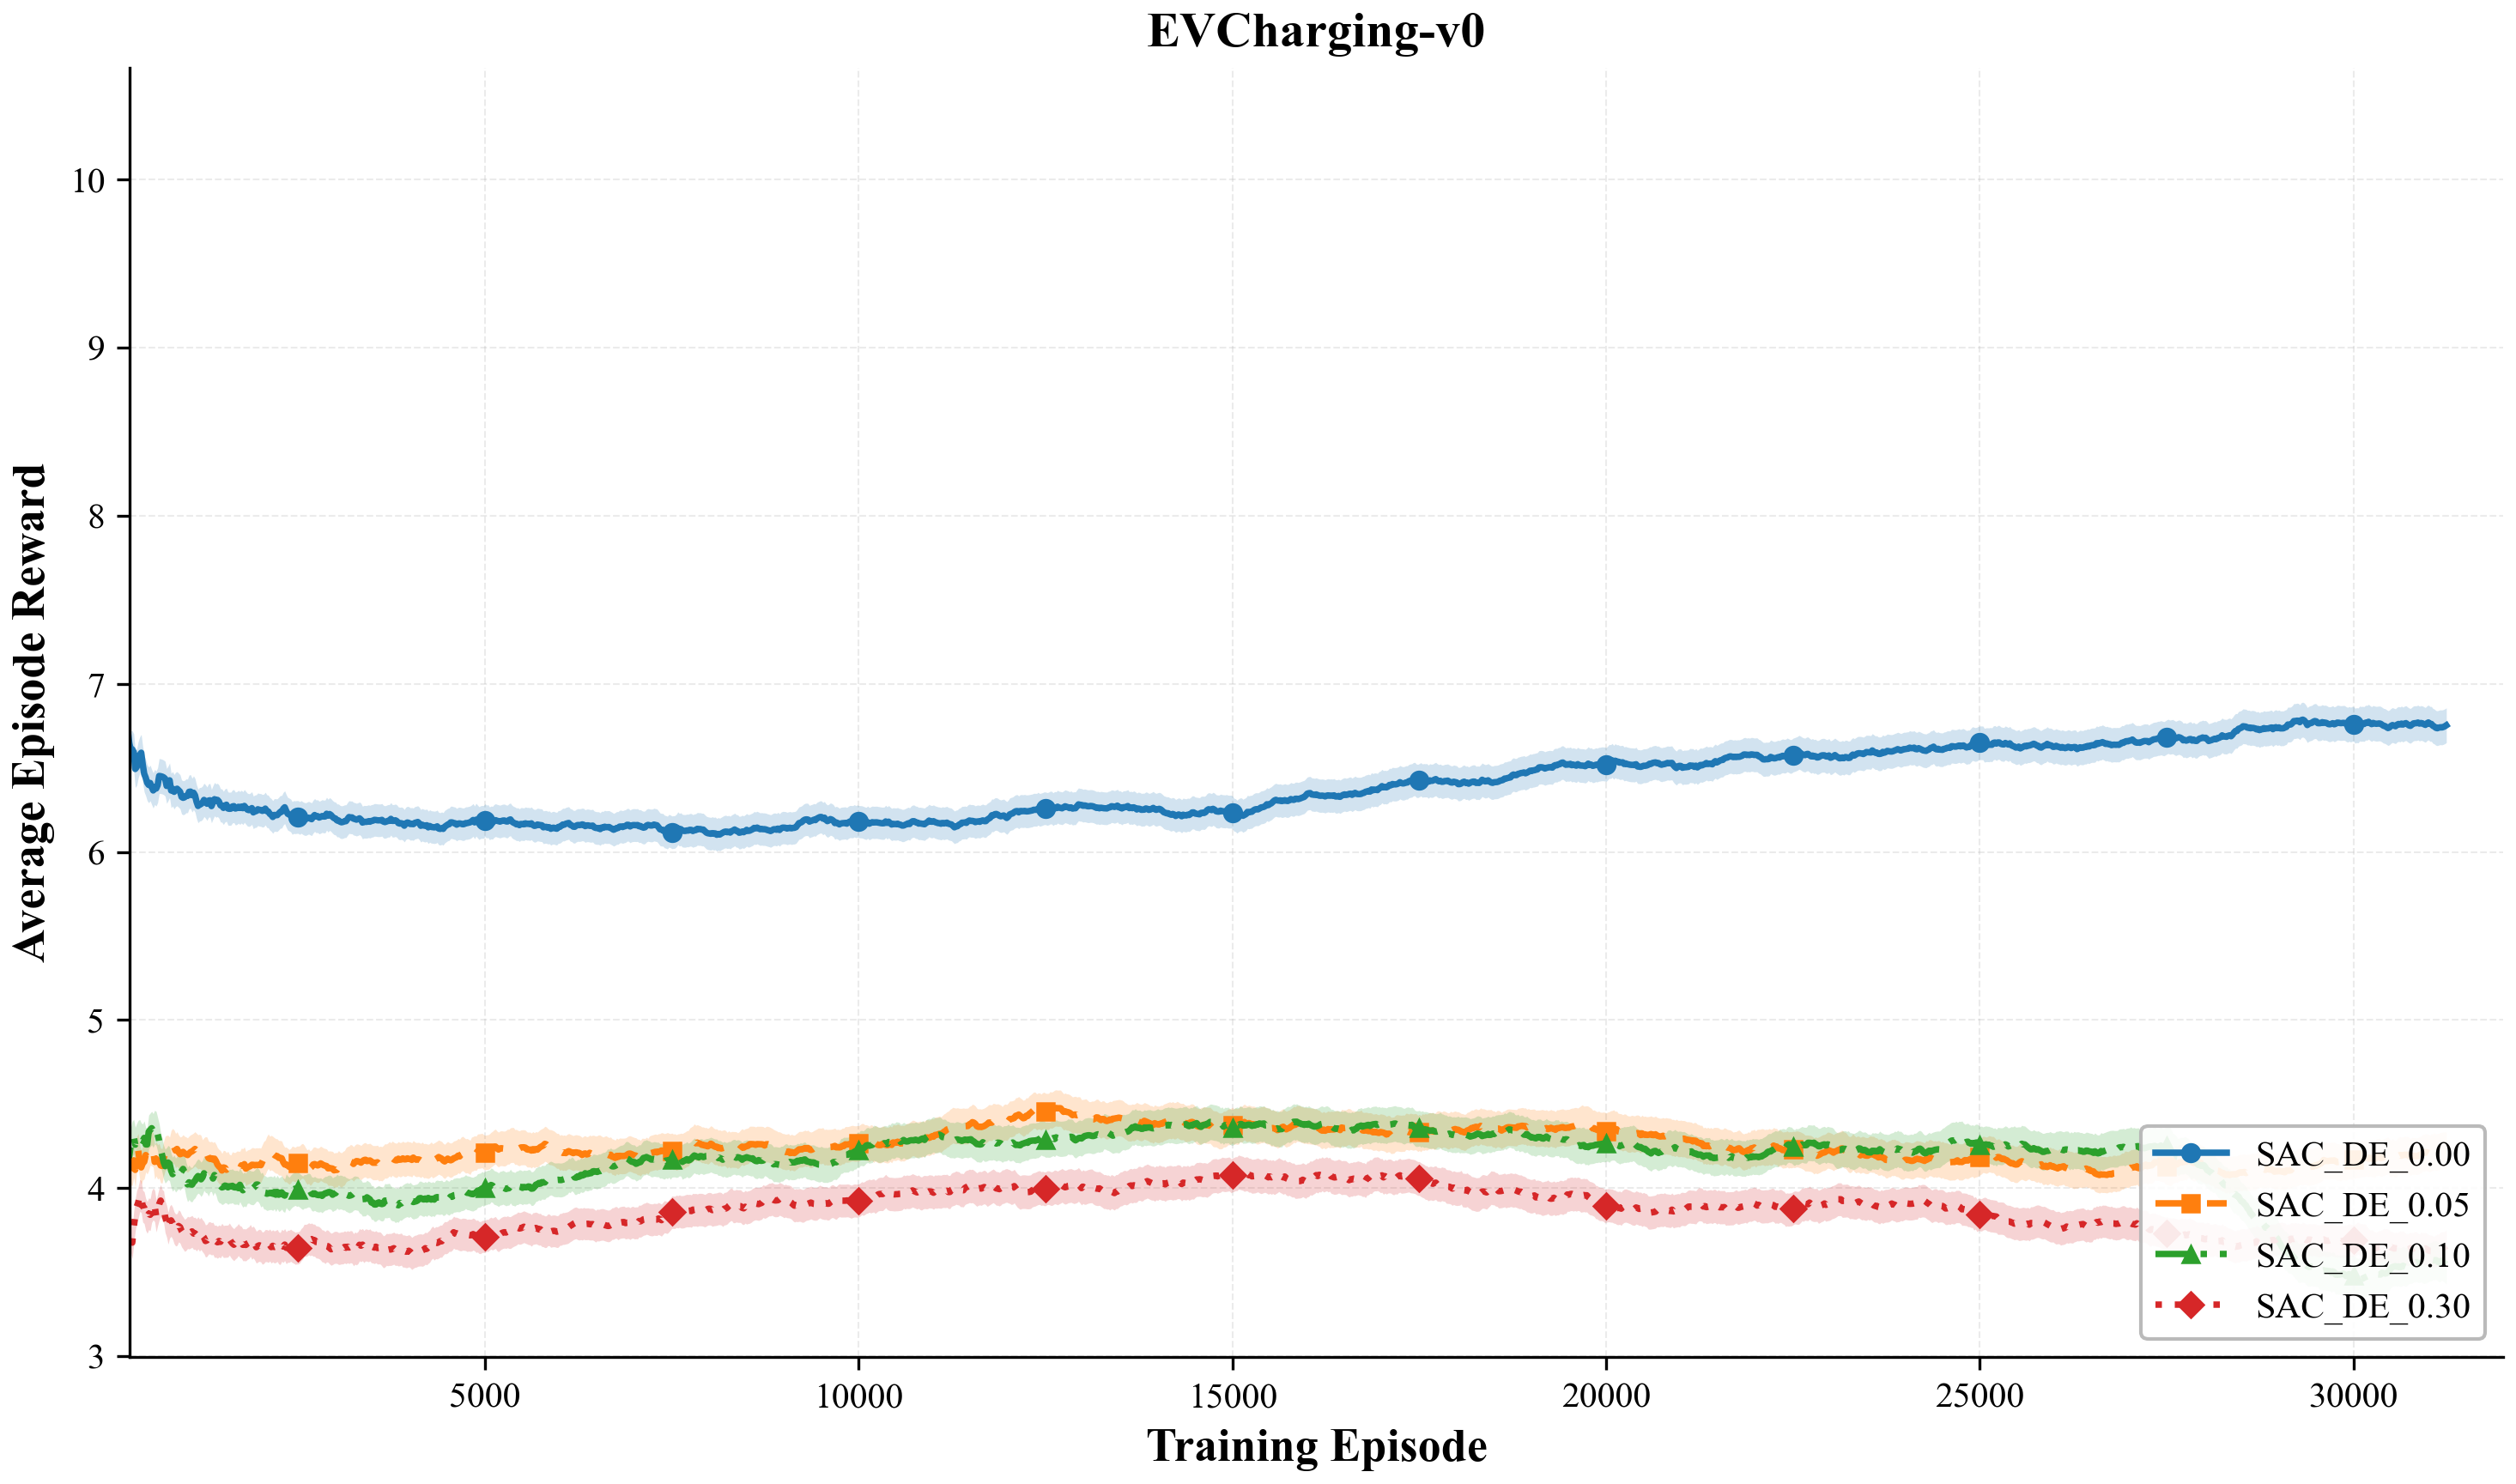
\includegraphics[width=0.9\textwidth]{figures/C_STDRL/ev/SAC/DE_2026-03-16_23-32-10.png}
\caption{EV Charging SAC: Training curves under environment noise (DE).}
\label{fig:stdrl_ev_sac_de}
\end{figure}

\paragraph{Test-time robustness.} Counterintuitively, SAC's performance \emph{improves} under observation noise (\Cref{fig:violin_ev_sac_obs}): the distribution shifts slightly rightward at higher noise levels, suggesting that noise acts as implicit regularization. SAC's entropy-based exploration benefits from additional stochasticity, preventing overfitting to specific EV arrival patterns.

\begin{figure}[htbp]
\centering

\includegraphics[width=0.9\textwidth]{figures/C_POST/evcharging/SAC/obs_violin.png}
\caption{EV Charging SAC: Reward distribution under observation noise. Slight rightward shift at higher noise suggests implicit regularization.}
\label{fig:violin_ev_sac_obs}
\end{figure}

\begin{figure}[htbp]
\centering

\includegraphics[width=0.9\textwidth]{figures/C_POST/evcharging/SAC/action_violin.png}
\caption{EV Charging SAC: Reward distribution under action noise.}
\label{fig:violin_ev_sac_act}
\end{figure}

\begin{figure}[htbp]
\centering

\includegraphics[width=0.9\textwidth]{figures/C_POST/evcharging/SAC/env_violin.png}
\caption{EV Charging SAC: Reward distribution under environment noise. Distribution broadens at high noise, indicating increased episode-to-episode variability in MOER-dependent rewards.}
\label{fig:violin_ev_sac_env}
\end{figure}

\begin{figure}[htbp]
\centering

\includegraphics[width=0.9\textwidth]{figures/C_POST/evcharging/SAC/panel.png}
\caption{EV Charging SAC: Summary panel across all three noise channels.}
\label{fig:post_ev_sac_panel}
\end{figure}

% ============================================================
\subsection{Building: Noise Robustness}
\label{sec:noise_bu}

The Building environment is the most noise-sensitive of the three environments, with rapid performance degradation under observation and environment noise. The RC thermal model amplifies per-timestep observation errors through coupled zone dynamics, creating cascading failures over the 288-step episode.

% --- Building PPO ---
\subsubsection{Building --- PPO}

\paragraph{Training curves.} \Cref{fig:stdrl_bu_ppo_ds} shows a clear separation between noise levels during training: higher observation noise leads to lower converged reward. Action noise (\Cref{fig:stdrl_bu_ppo_da}) and environment noise (\Cref{fig:stdrl_bu_ppo_de}) show similar but more severe training degradation patterns.

\begin{figure}[htbp]
\centering
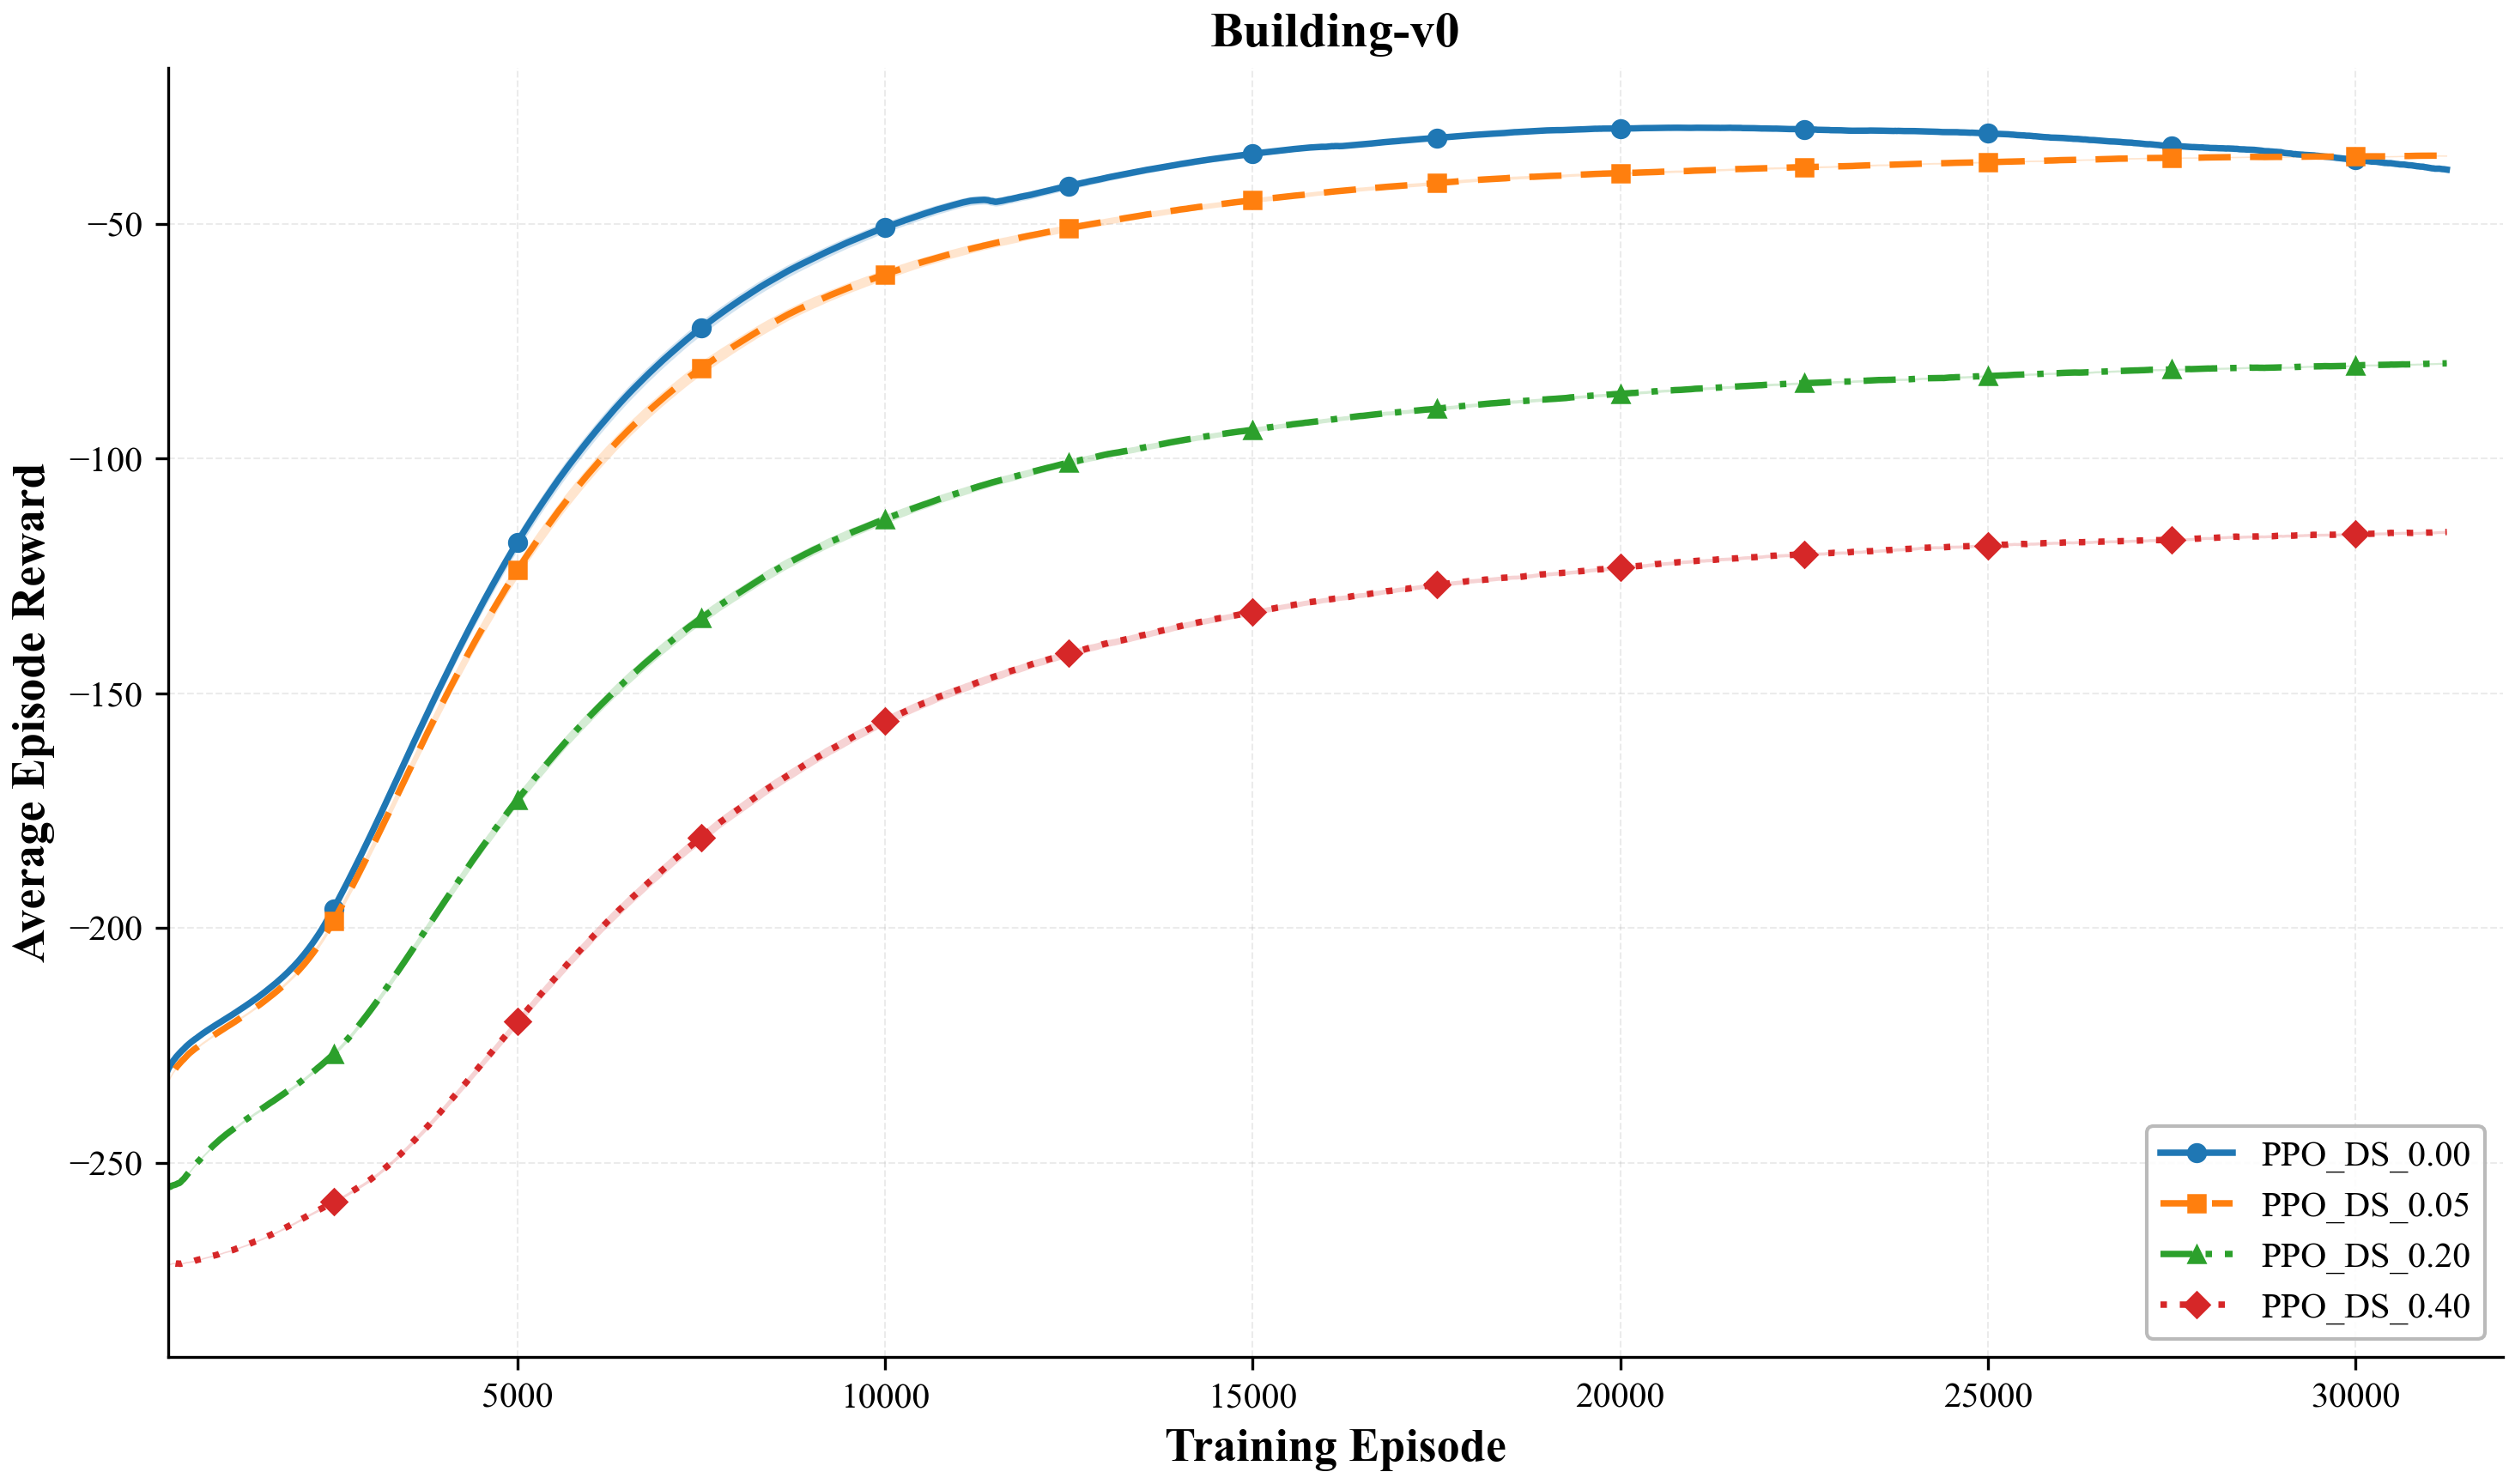
\includegraphics[width=0.9\textwidth]{figures/C_STDRL/bu/PPO/DS_2026-03-16_23-32-18.png}
\caption{Building PPO: Training curves under observation noise (DS).}
\label{fig:stdrl_bu_ppo_ds}
\end{figure}

\begin{figure}[htbp]
\centering
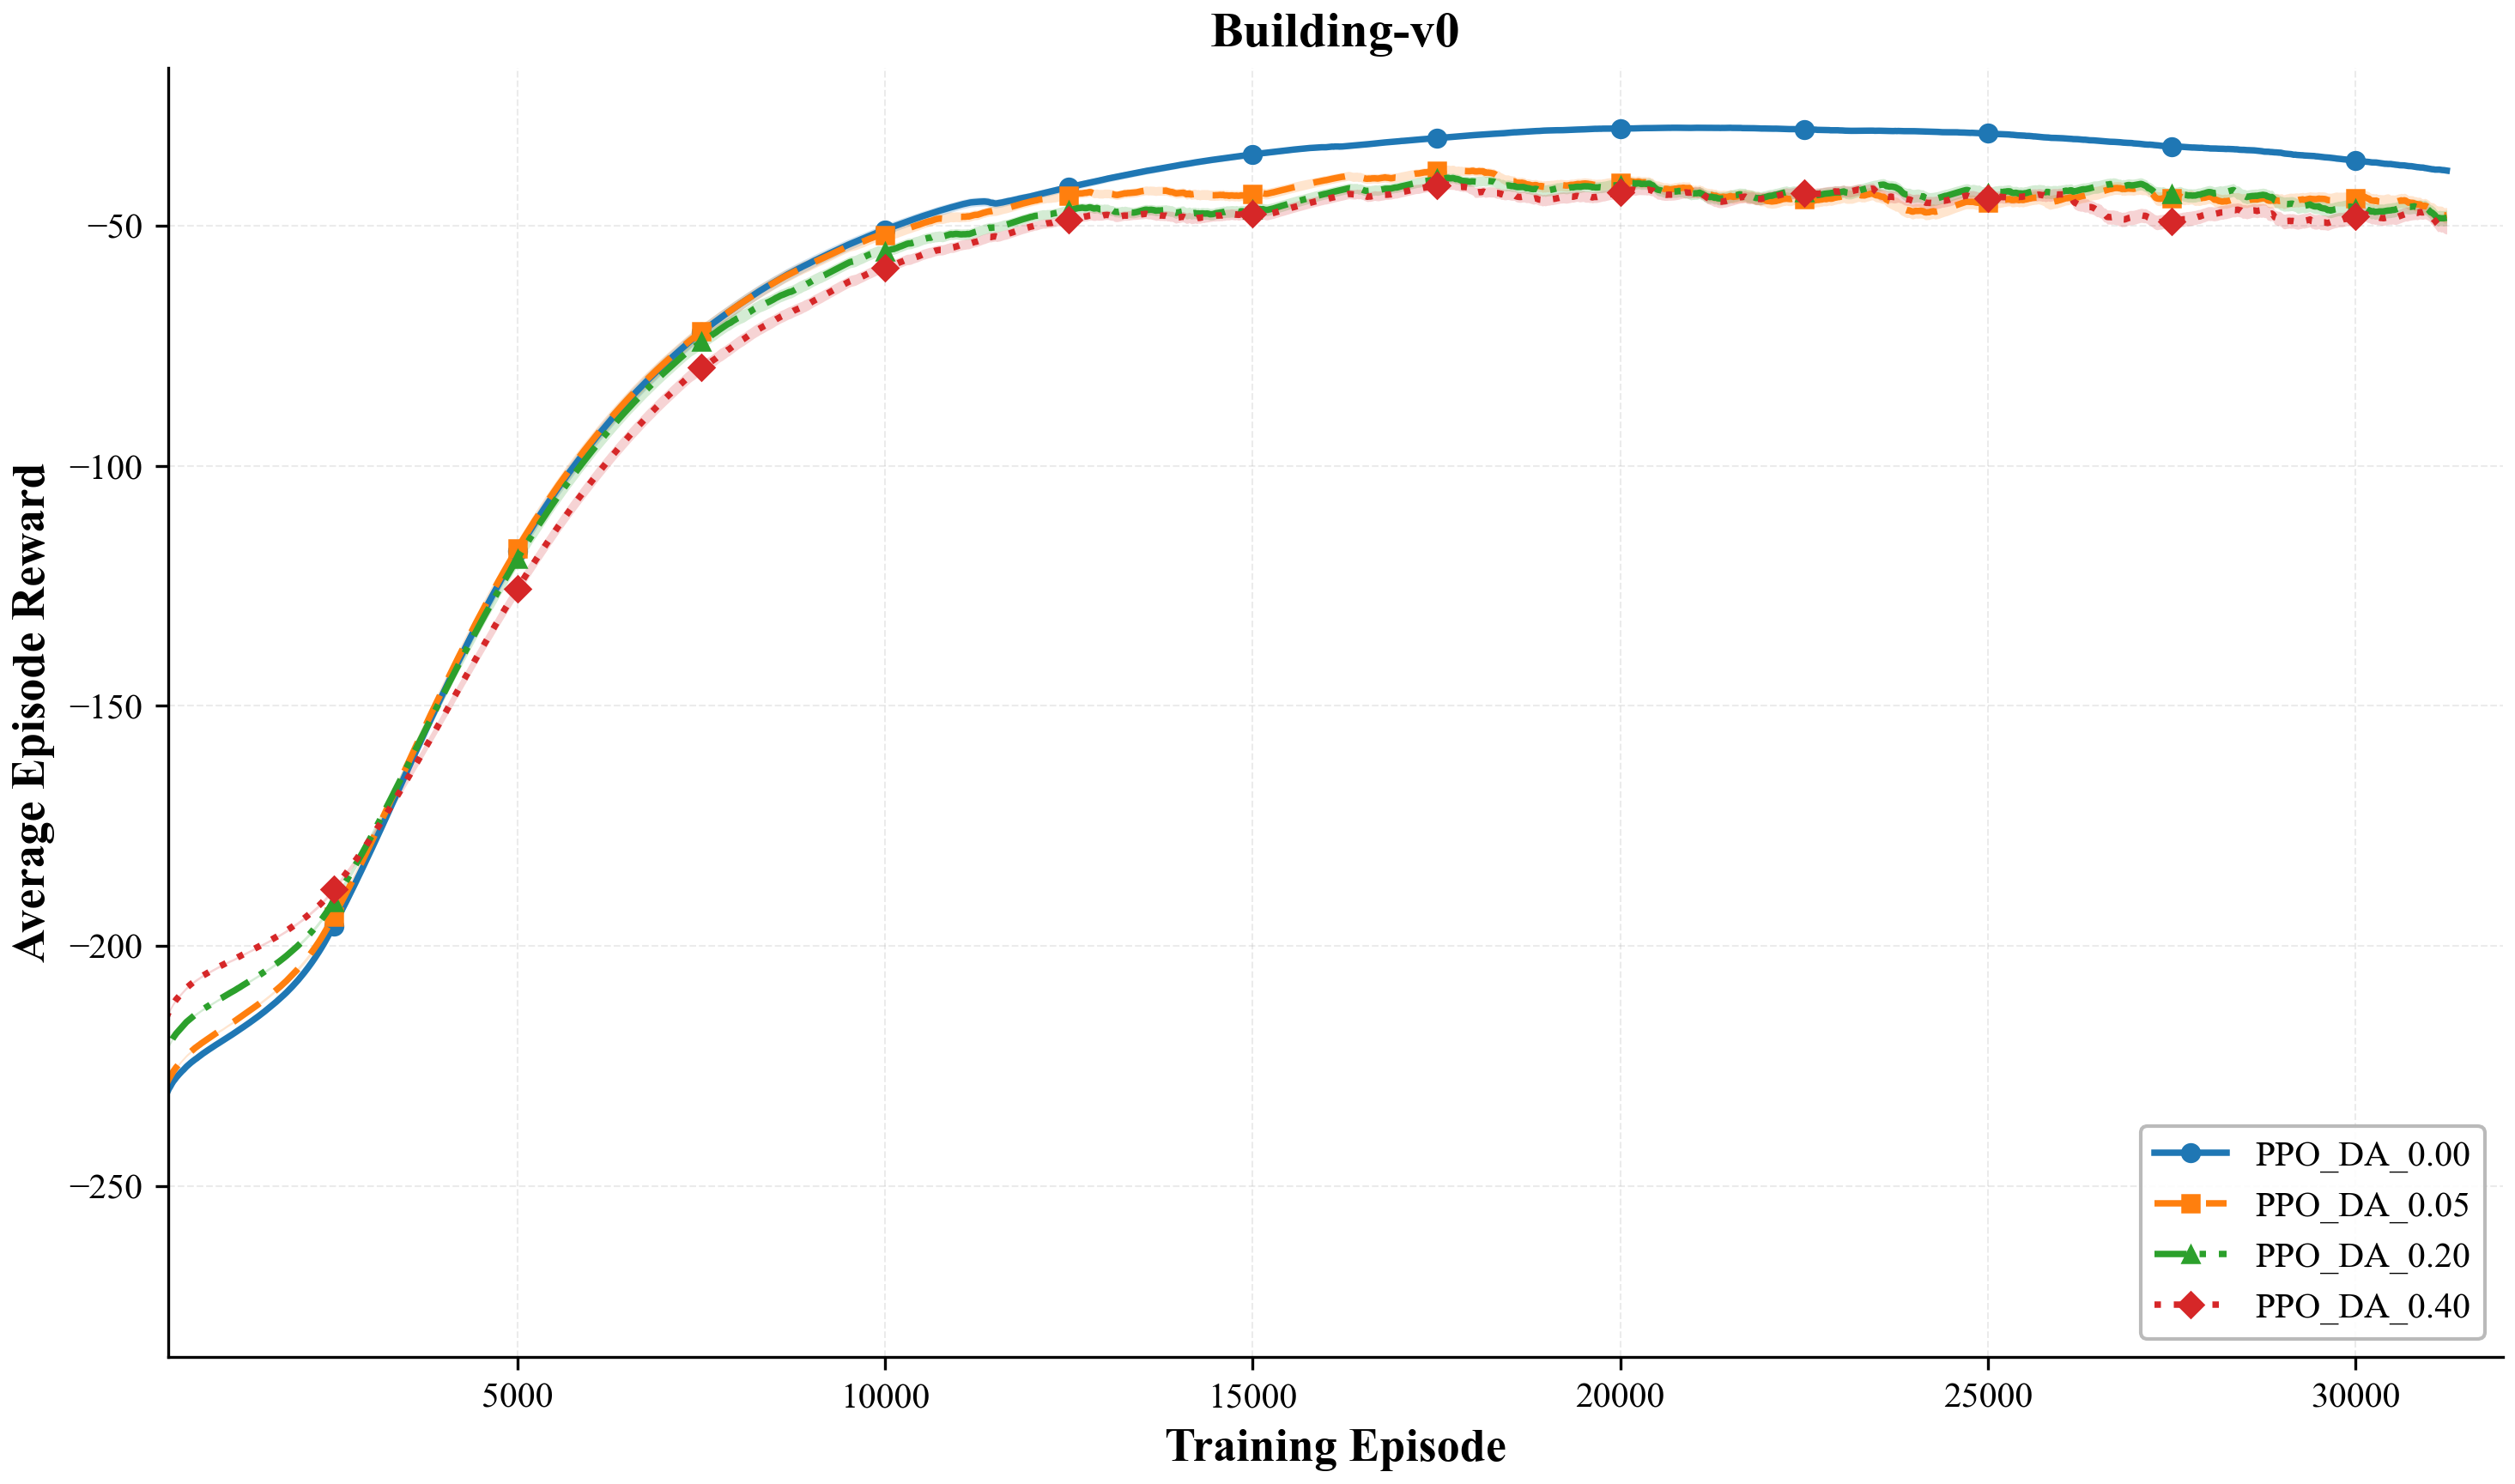
\includegraphics[width=0.9\textwidth]{figures/C_STDRL/bu/PPO/DA_2026-03-16_23-32-19.png}
\caption{Building PPO: Training curves under action noise (DA).}
\label{fig:stdrl_bu_ppo_da}
\end{figure}

\begin{figure}[htbp]
\centering
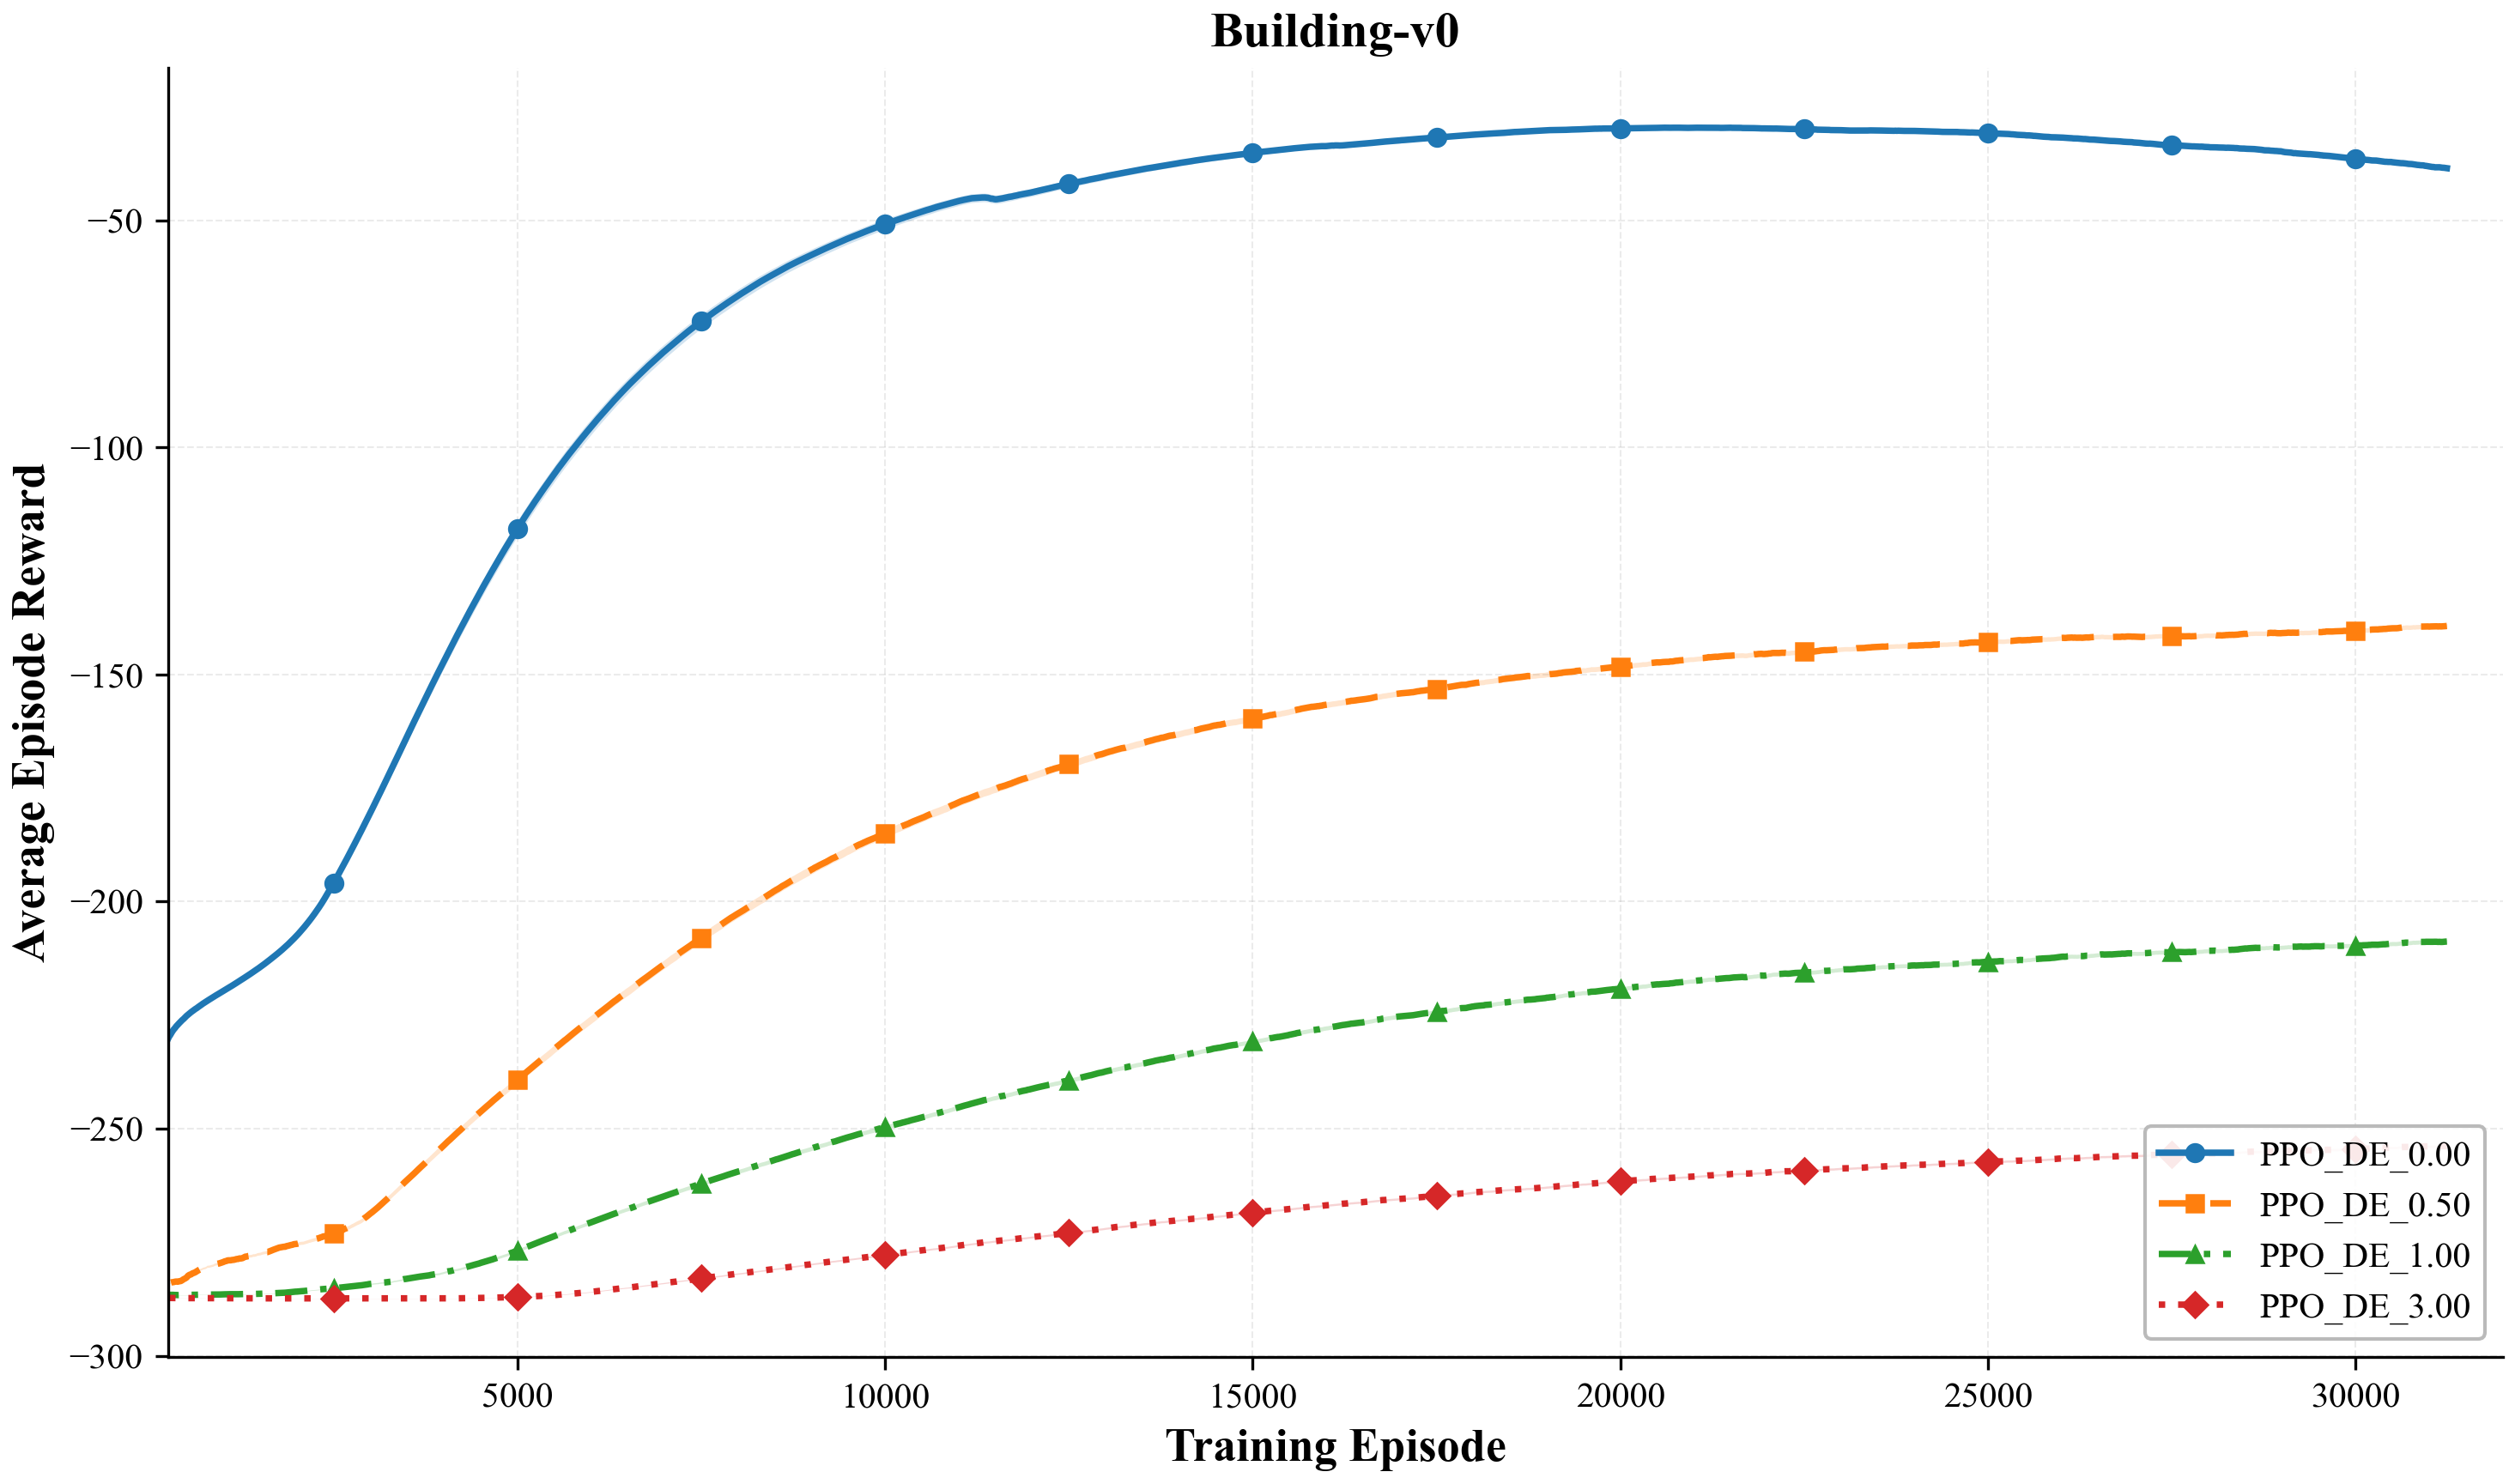
\includegraphics[width=0.9\textwidth]{figures/C_STDRL/bu/PPO/DE_2026-03-16_23-32-21.png}
\caption{Building PPO: Training curves under environment noise (DE).}
\label{fig:stdrl_bu_ppo_de}
\end{figure}

\paragraph{Test-time robustness.} The violin plots reveal the distributional impact of noise. Under observation noise (\Cref{fig:violin_bu_ppo_obs}), the bimodal reward structure---driven by high-occupancy vs.\ low-occupancy days---shifts entirely downward at $\sigma \geq 0.15$, with the high-reward mode collapsing. Under action noise (\Cref{fig:violin_bu_ppo_act}), the distribution shape is largely preserved up to $\sigma_{\text{act}} = 0.2$, consistent with the HVAC system's bang-bang control nature. Under environment noise (\Cref{fig:violin_bu_ppo_env}), the entire distribution collapses catastrophically as thermal dynamics amplify weather prediction errors.

\begin{figure}[htbp]
\centering
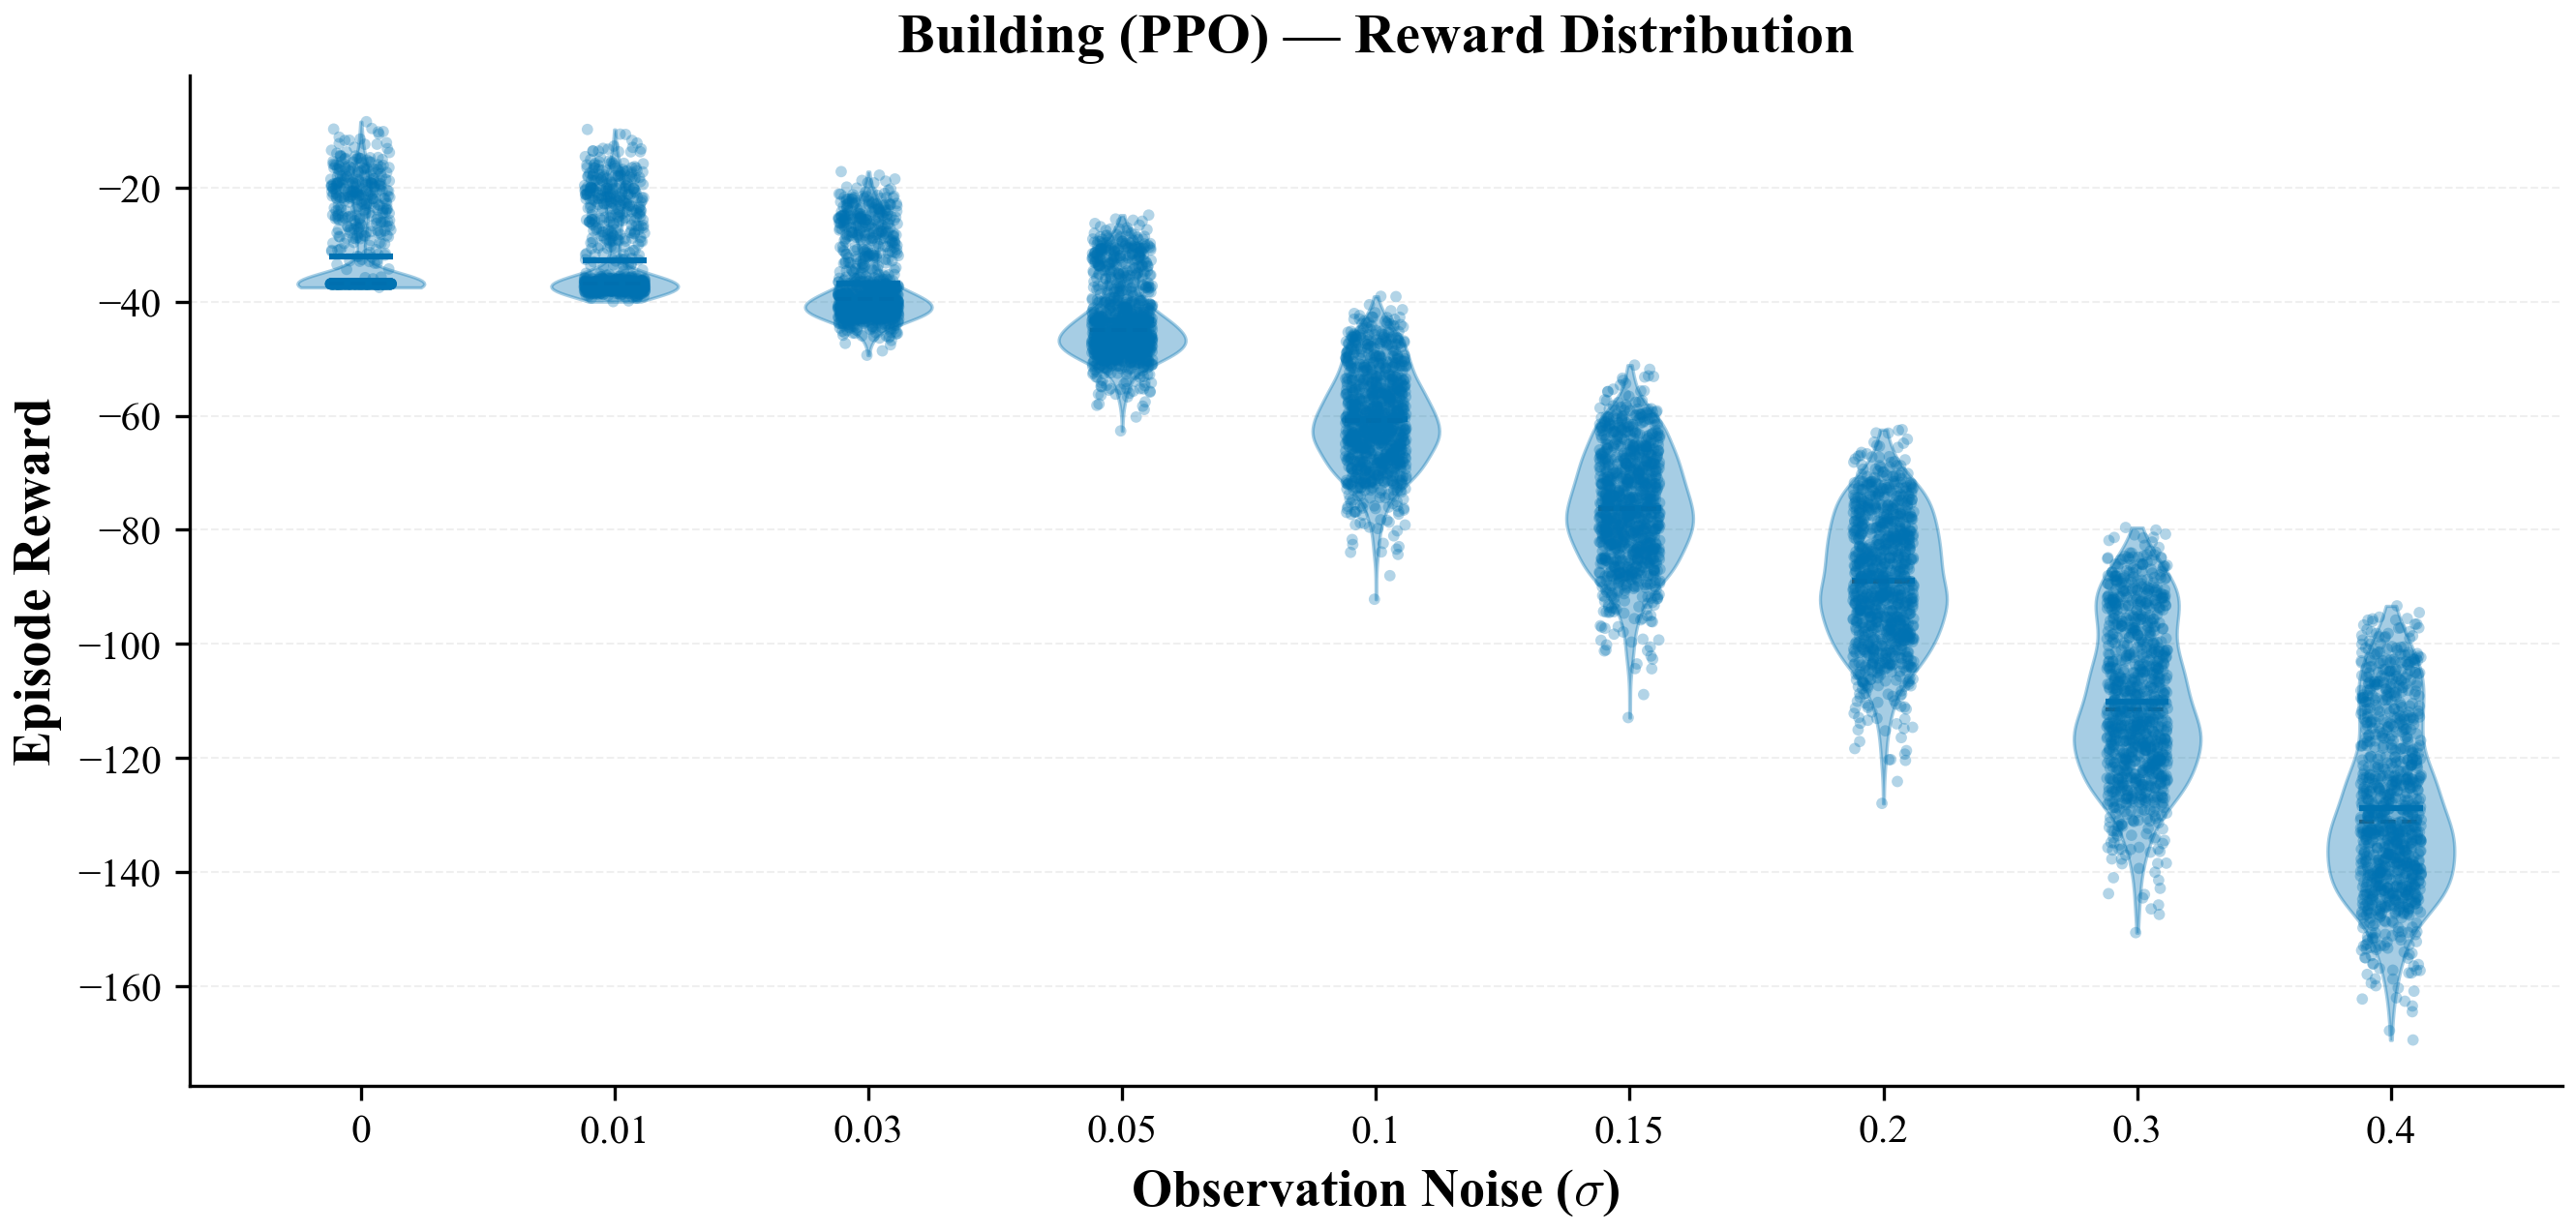
\includegraphics[width=0.9\textwidth]{figures/C_POST/building/PPO/obs_violin.png}
\caption{Building PPO: Reward distribution under observation noise. The bimodal structure shifts downward with increasing noise; the high-reward mode collapses at $\sigma \geq 0.15$.}
\label{fig:violin_bu_ppo_obs}
\end{figure}

\begin{figure}[htbp]
\centering
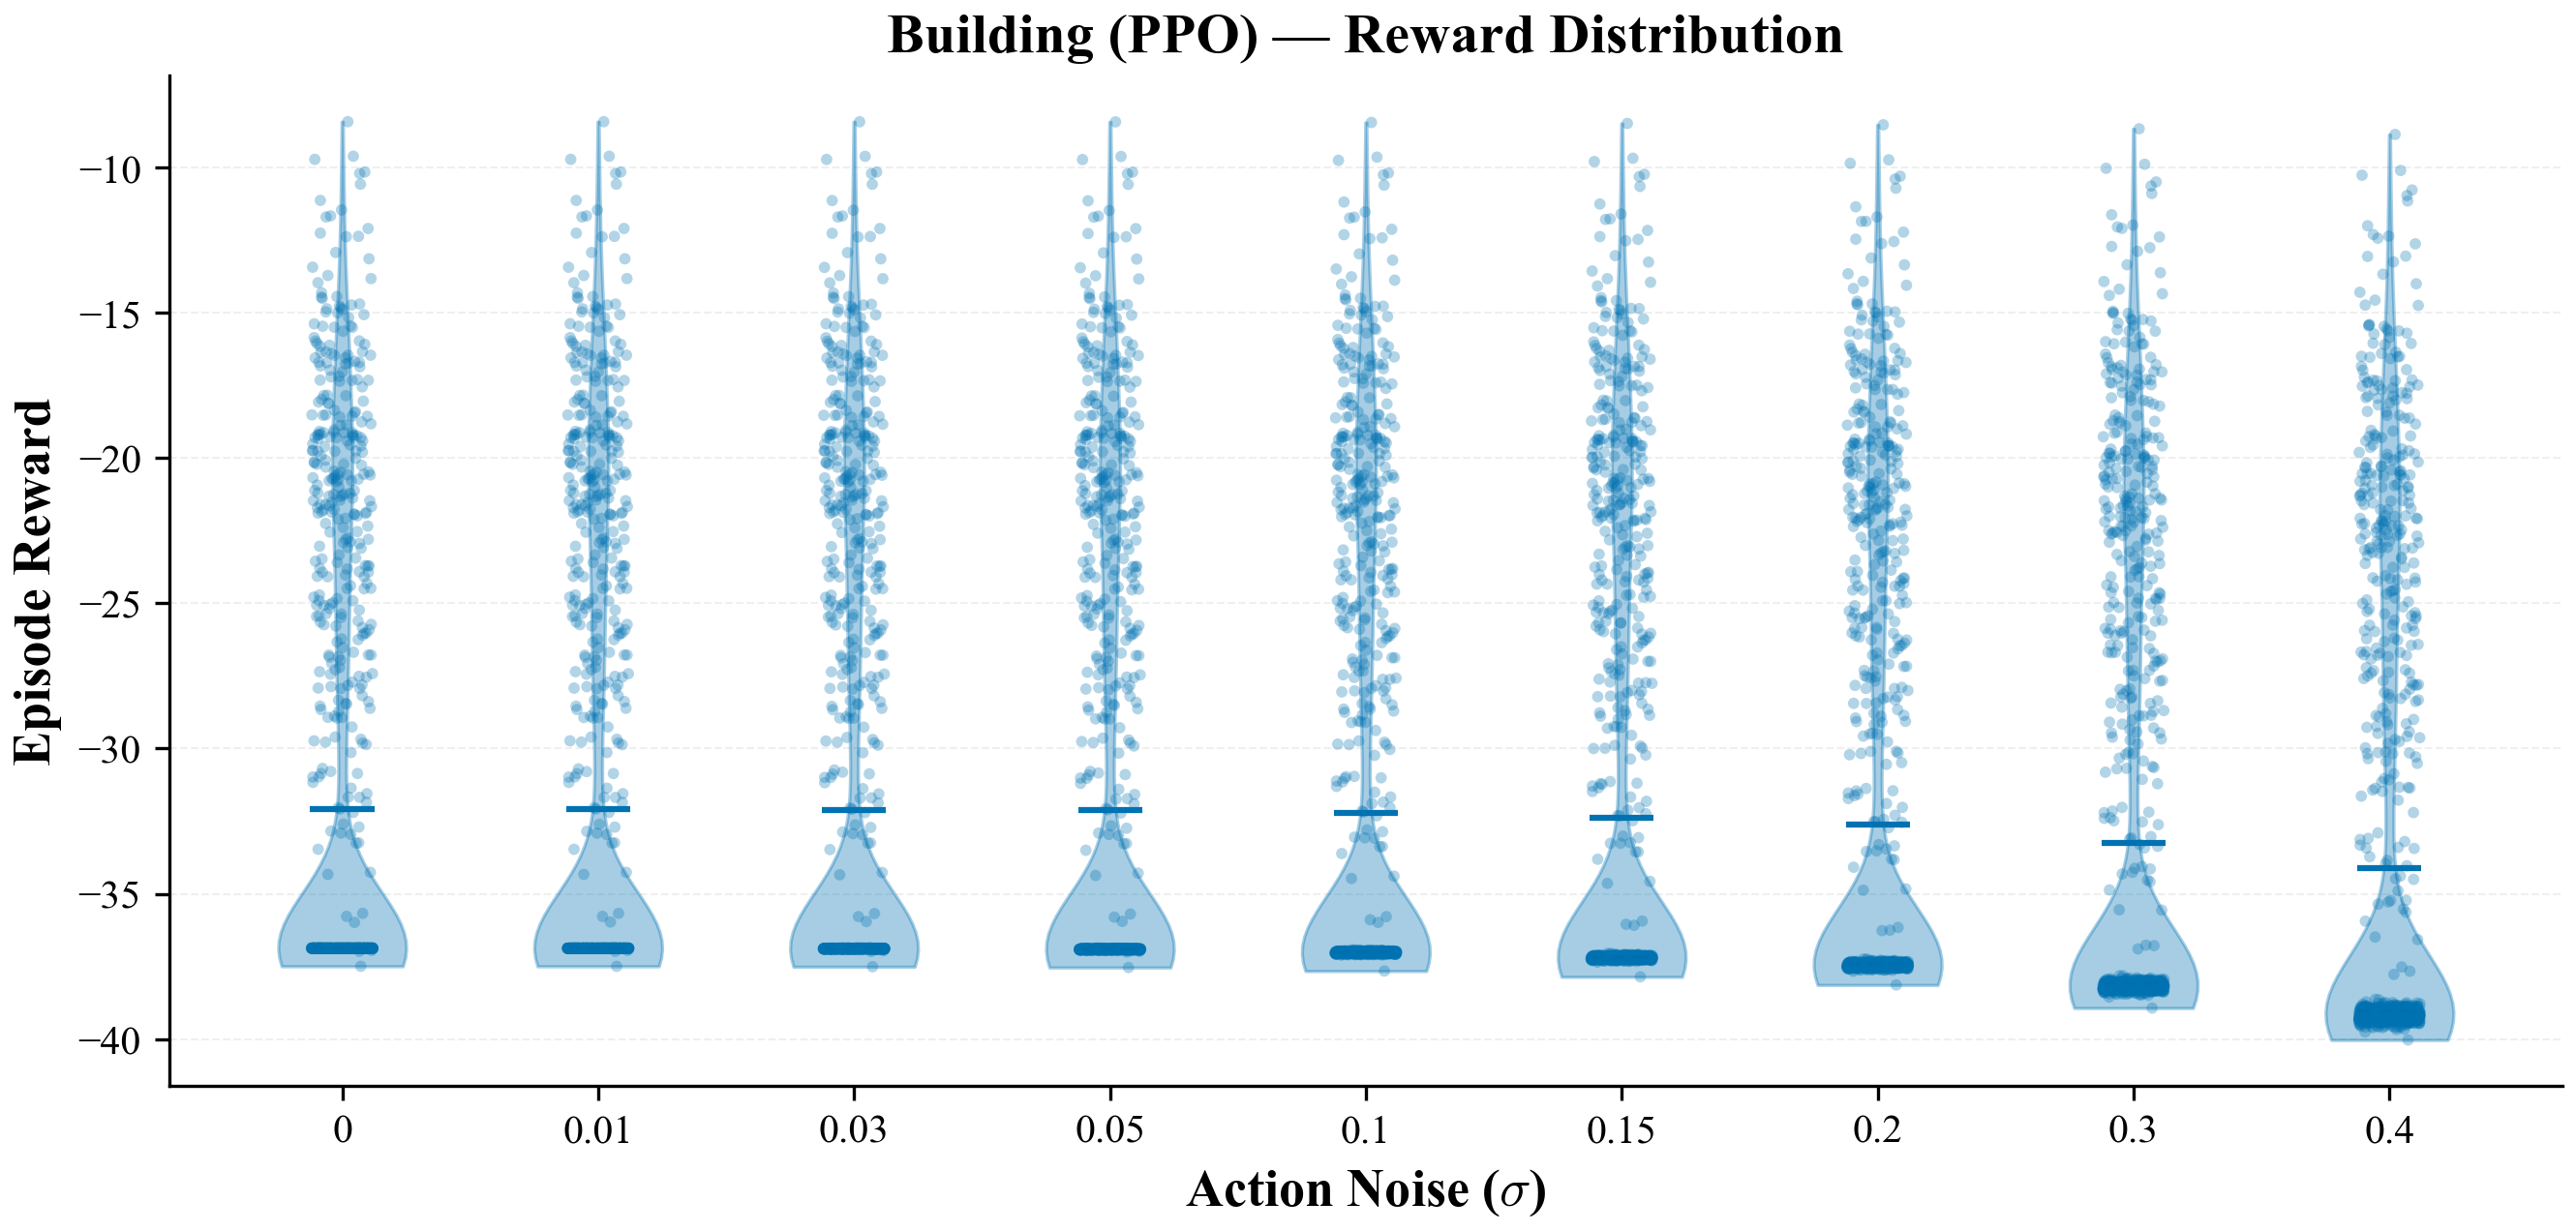
\includegraphics[width=0.9\textwidth]{figures/C_POST/building/PPO/action_violin.png}
\caption{Building PPO: Reward distribution under action noise. Distribution shape preserved up to $\sigma_{\text{act}} = 0.2$, consistent with bang-bang HVAC control.}
\label{fig:violin_bu_ppo_act}
\end{figure}

\begin{figure}[htbp]
\centering
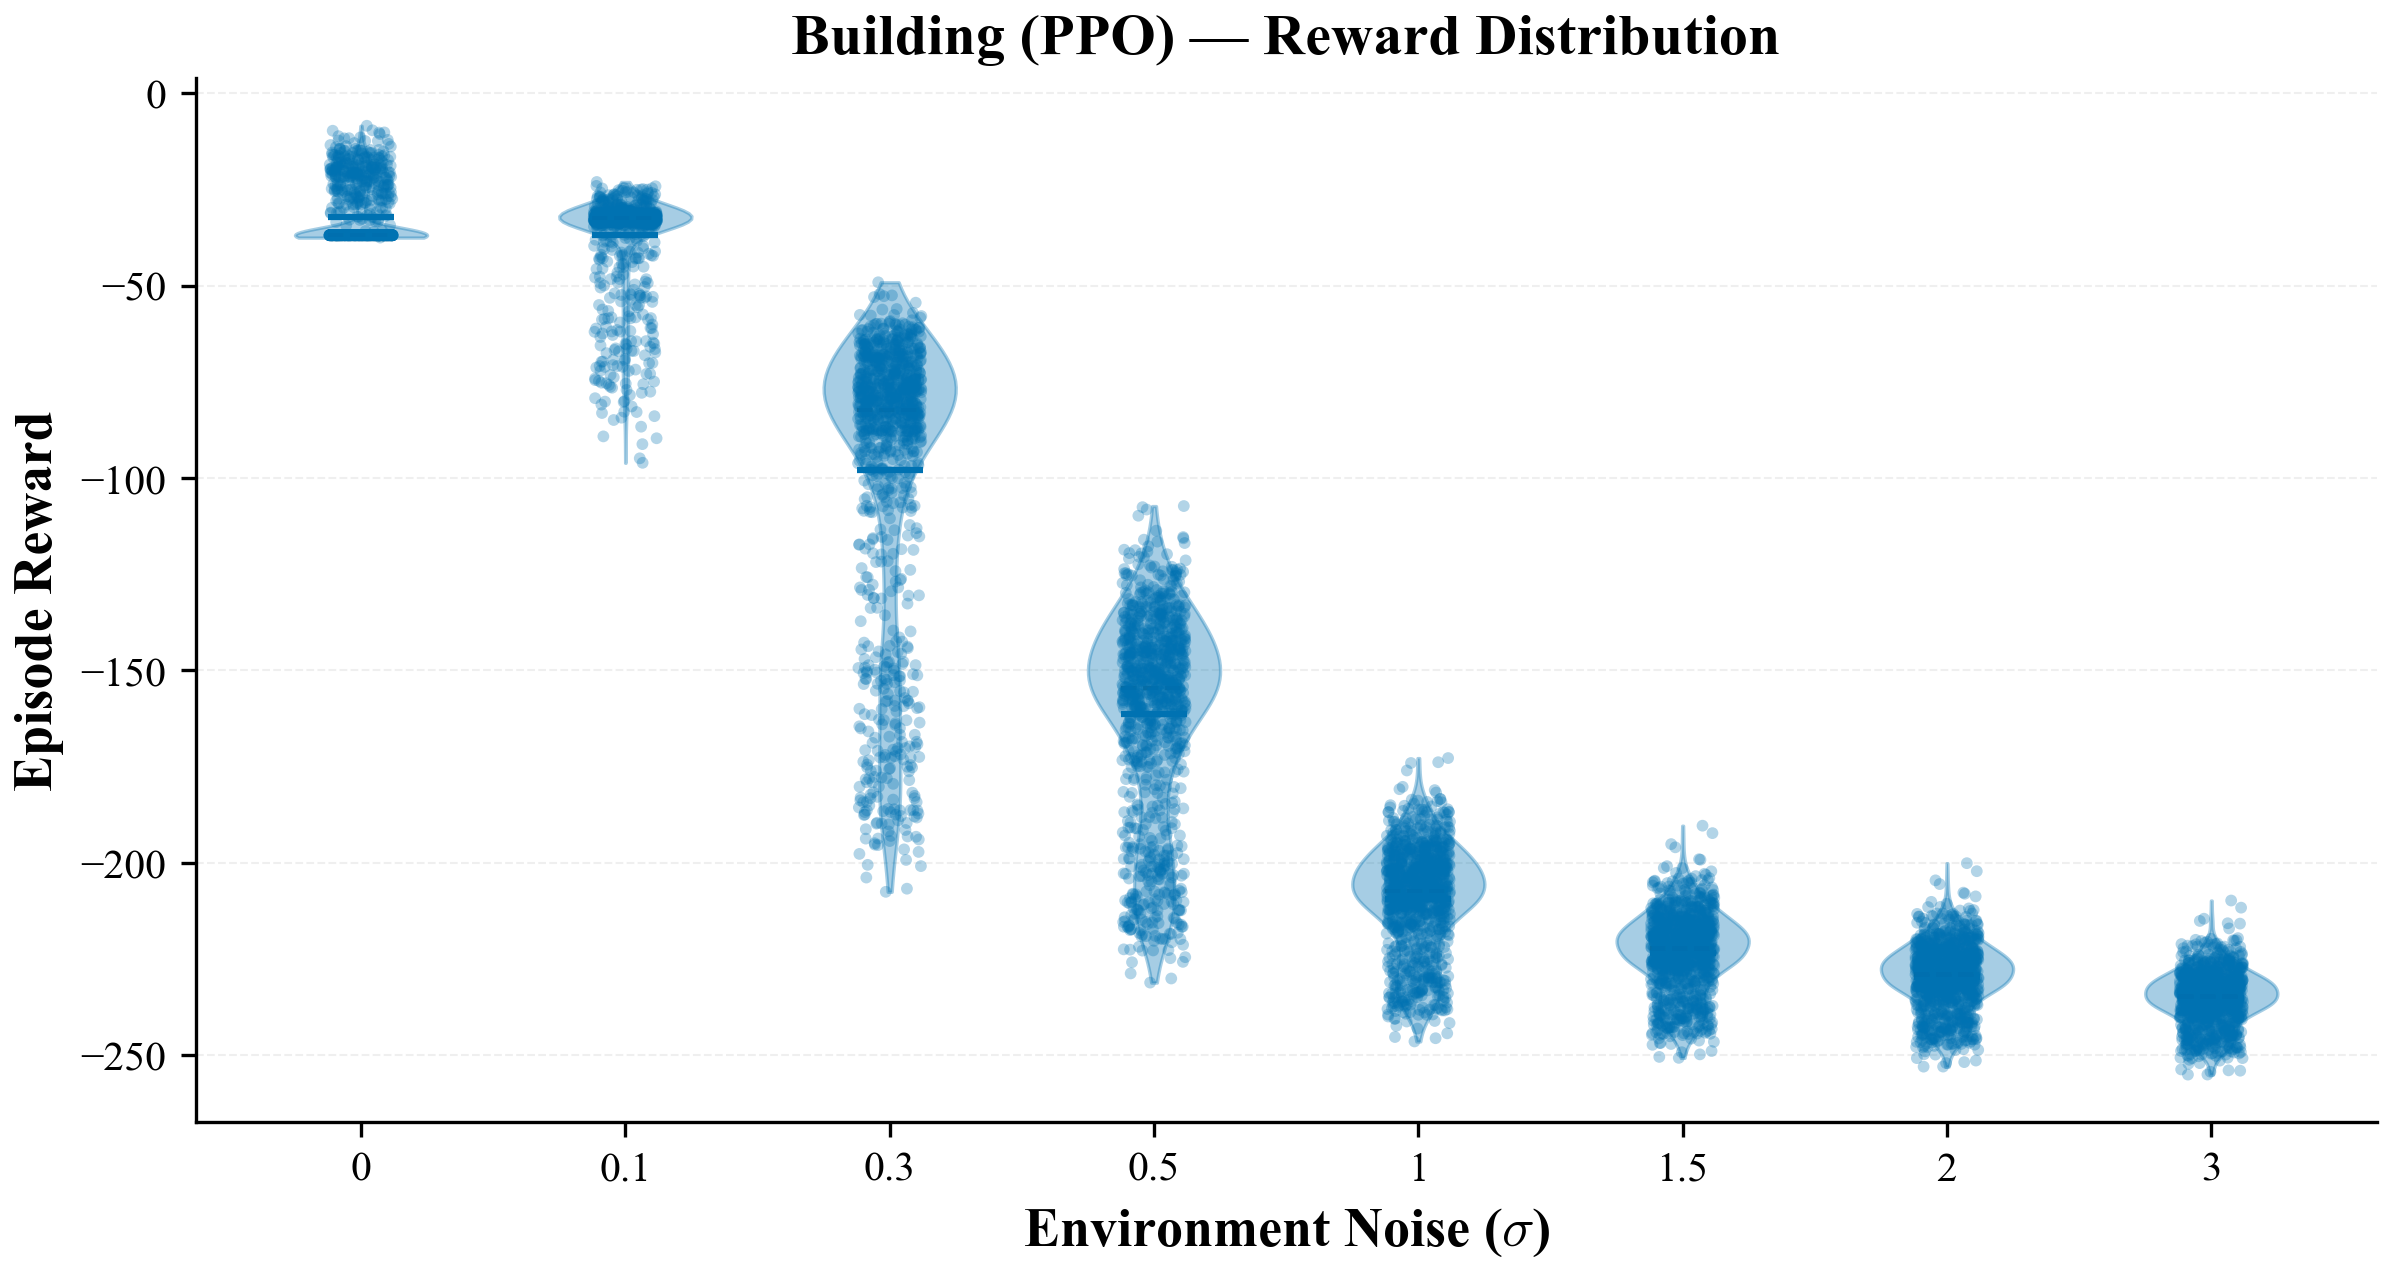
\includegraphics[width=0.9\textwidth]{figures/C_POST/building/PPO/env_violin.png}
\caption{Building PPO: Reward distribution under environment noise. Catastrophic degradation: the entire distribution collapses as thermal dynamics amplify weather prediction errors.}
\label{fig:violin_bu_ppo_env}
\end{figure}

\begin{figure}[htbp]
\centering
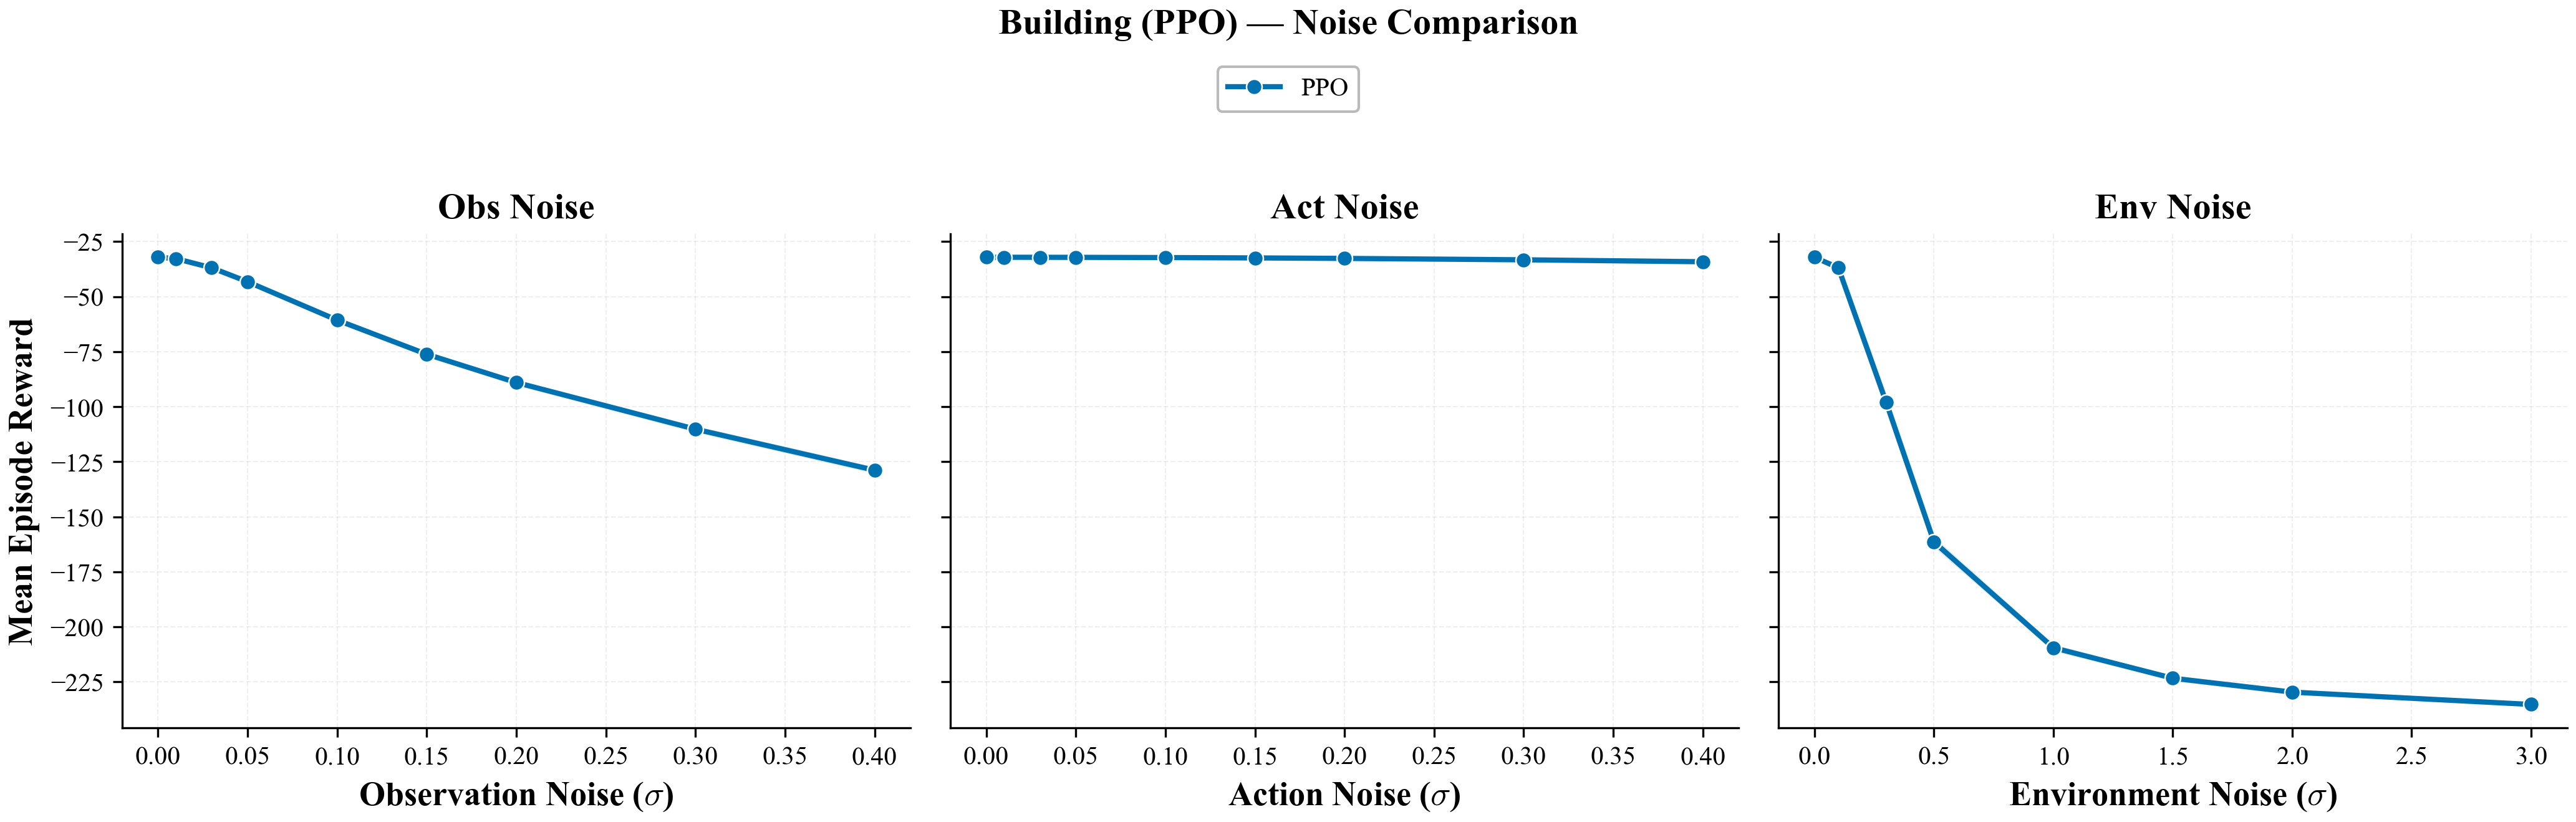
\includegraphics[width=0.9\textwidth]{figures/C_POST/building/PPO/panel.png}
\caption{Building PPO: Summary panel. Observation and environment noise cause severe degradation; action noise has minimal impact.}
\label{fig:post_bu_ppo_panel}
\end{figure}

% --- Building SAC ---
\subsubsection{Building --- SAC}

\paragraph{Training curves.} SAC's training curves (\Cref{fig:stdrl_bu_sac_ds,fig:stdrl_bu_sac_da,fig:stdrl_bu_sac_de}) show a similar pattern to PPO but with lower absolute performance due to SAC's weaker baseline in this environment.

\begin{figure}[htbp]
\centering
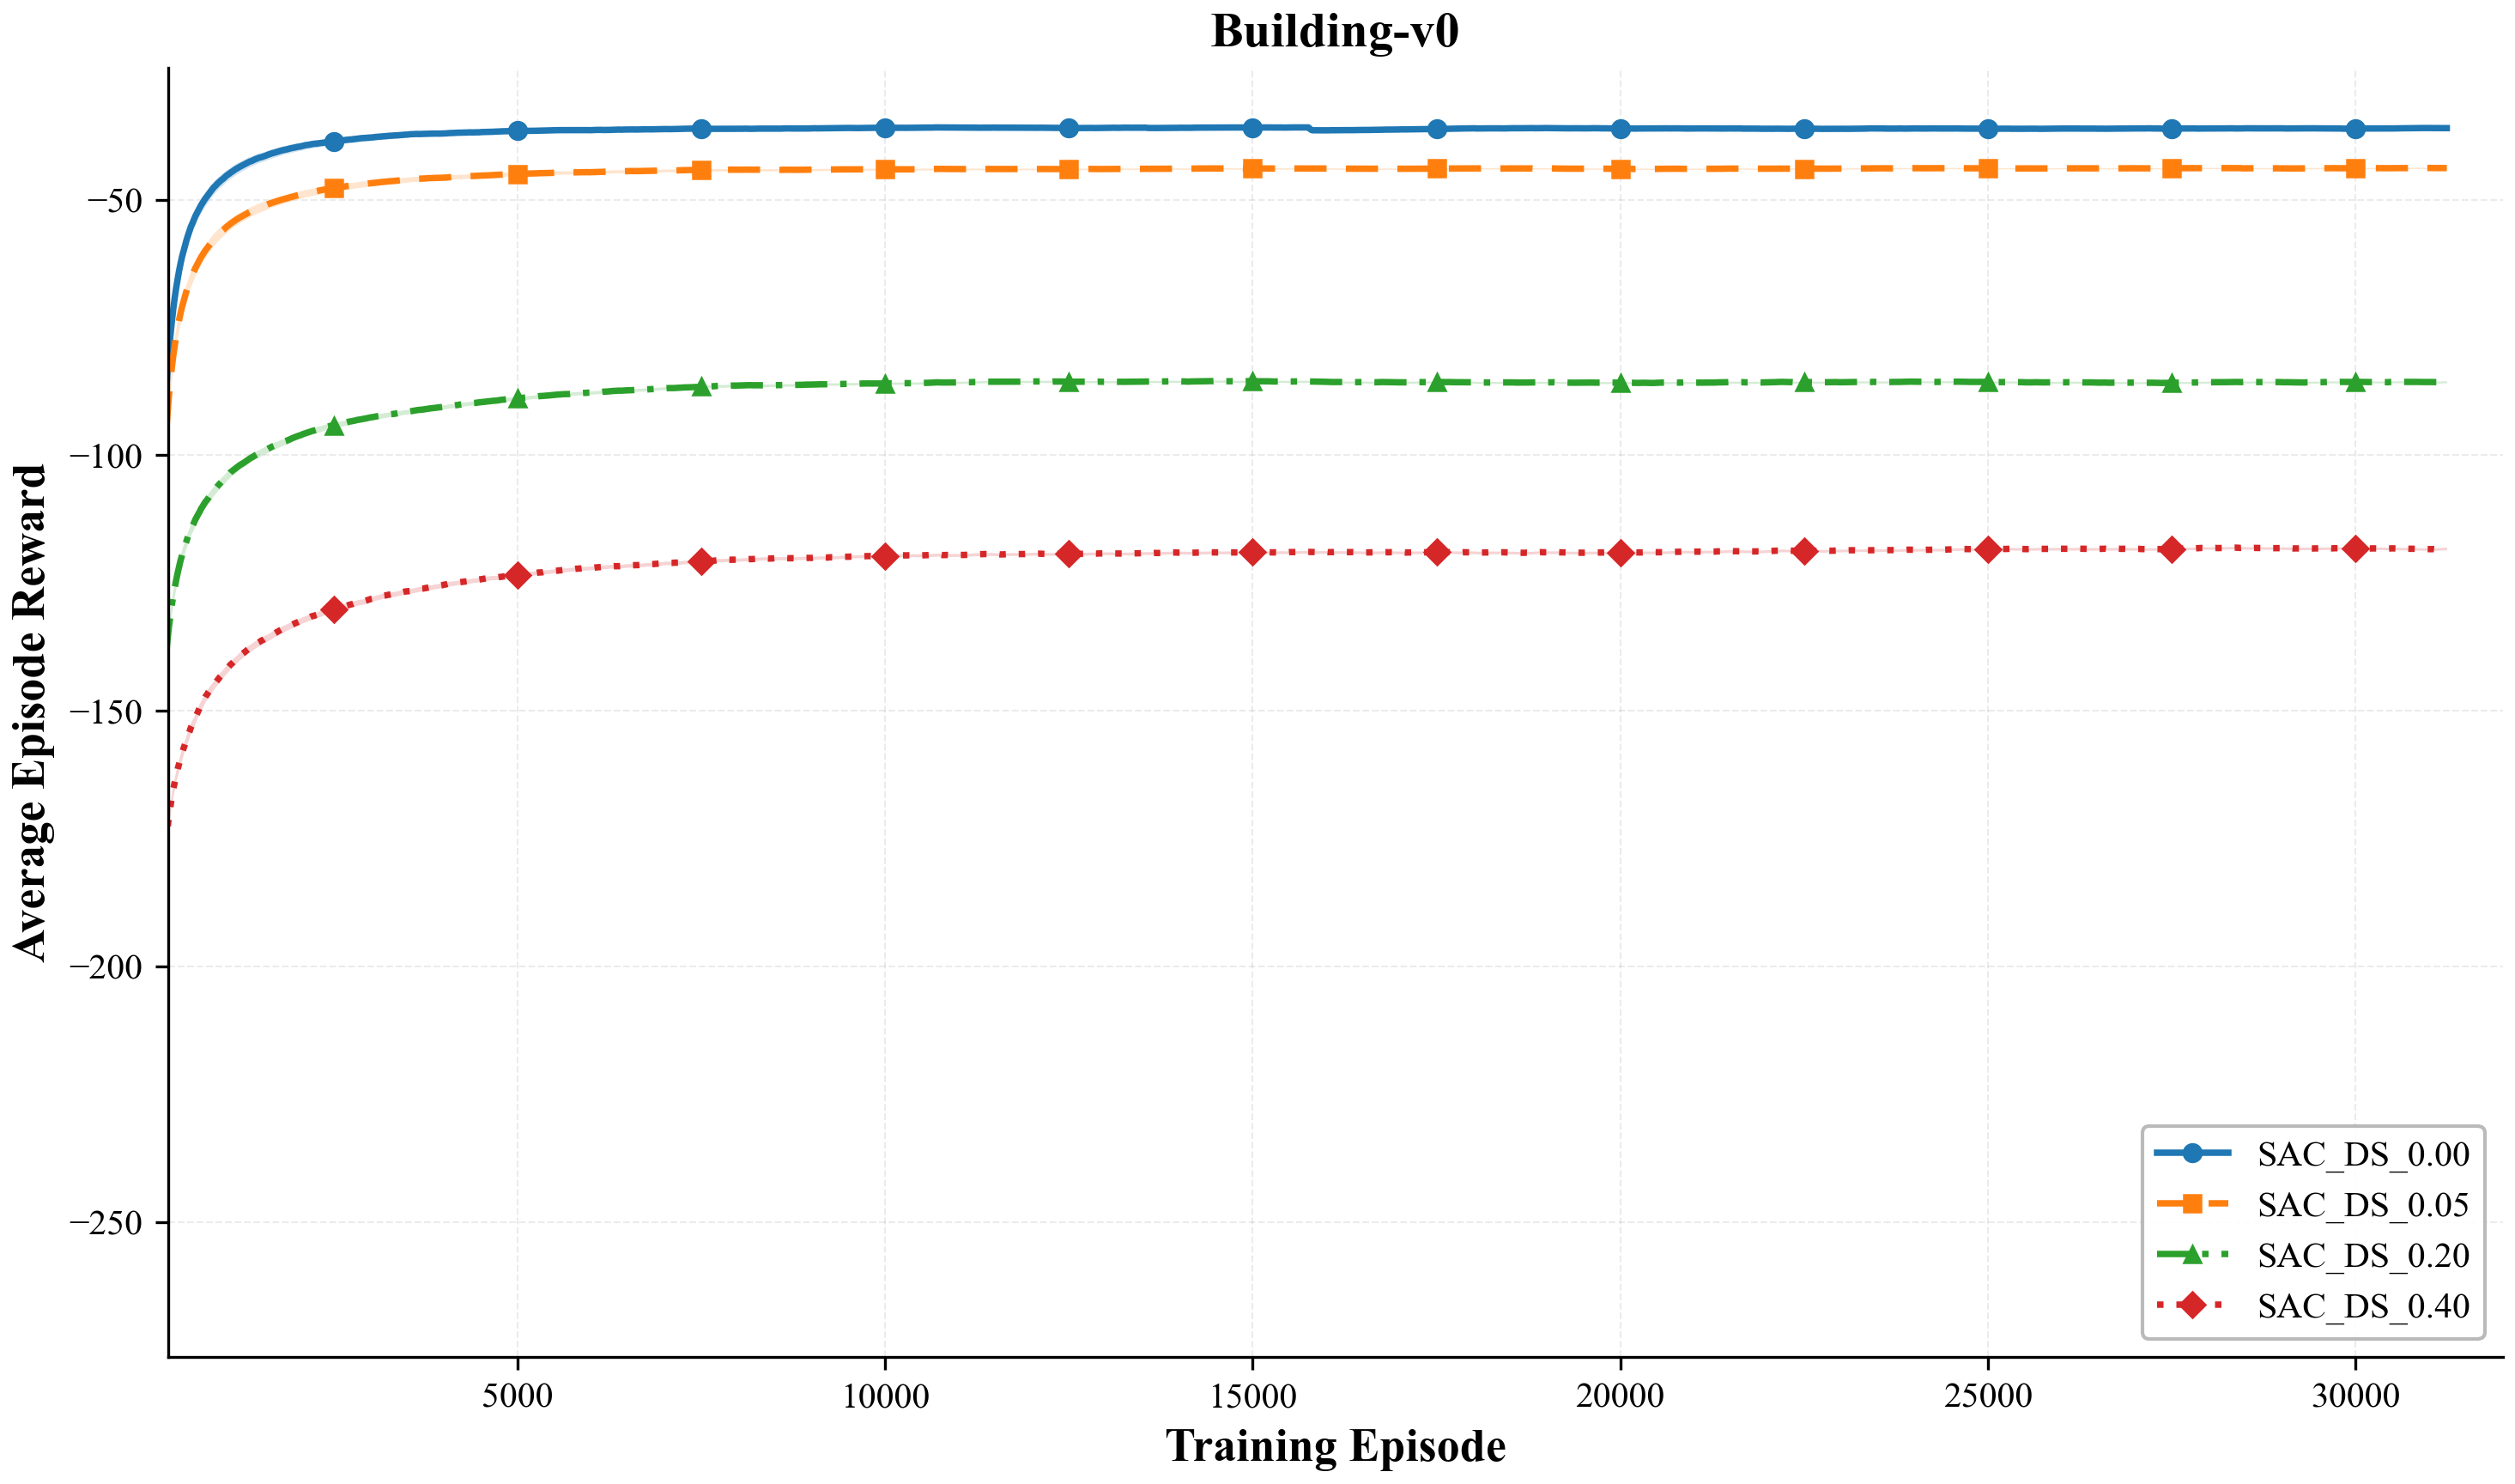
\includegraphics[width=0.9\textwidth]{figures/C_STDRL/bu/SAC/DS_2026-03-16_23-32-23.png}
\caption{Building SAC: Training curves under observation noise (DS).}
\label{fig:stdrl_bu_sac_ds}
\end{figure}

\begin{figure}[htbp]
\centering
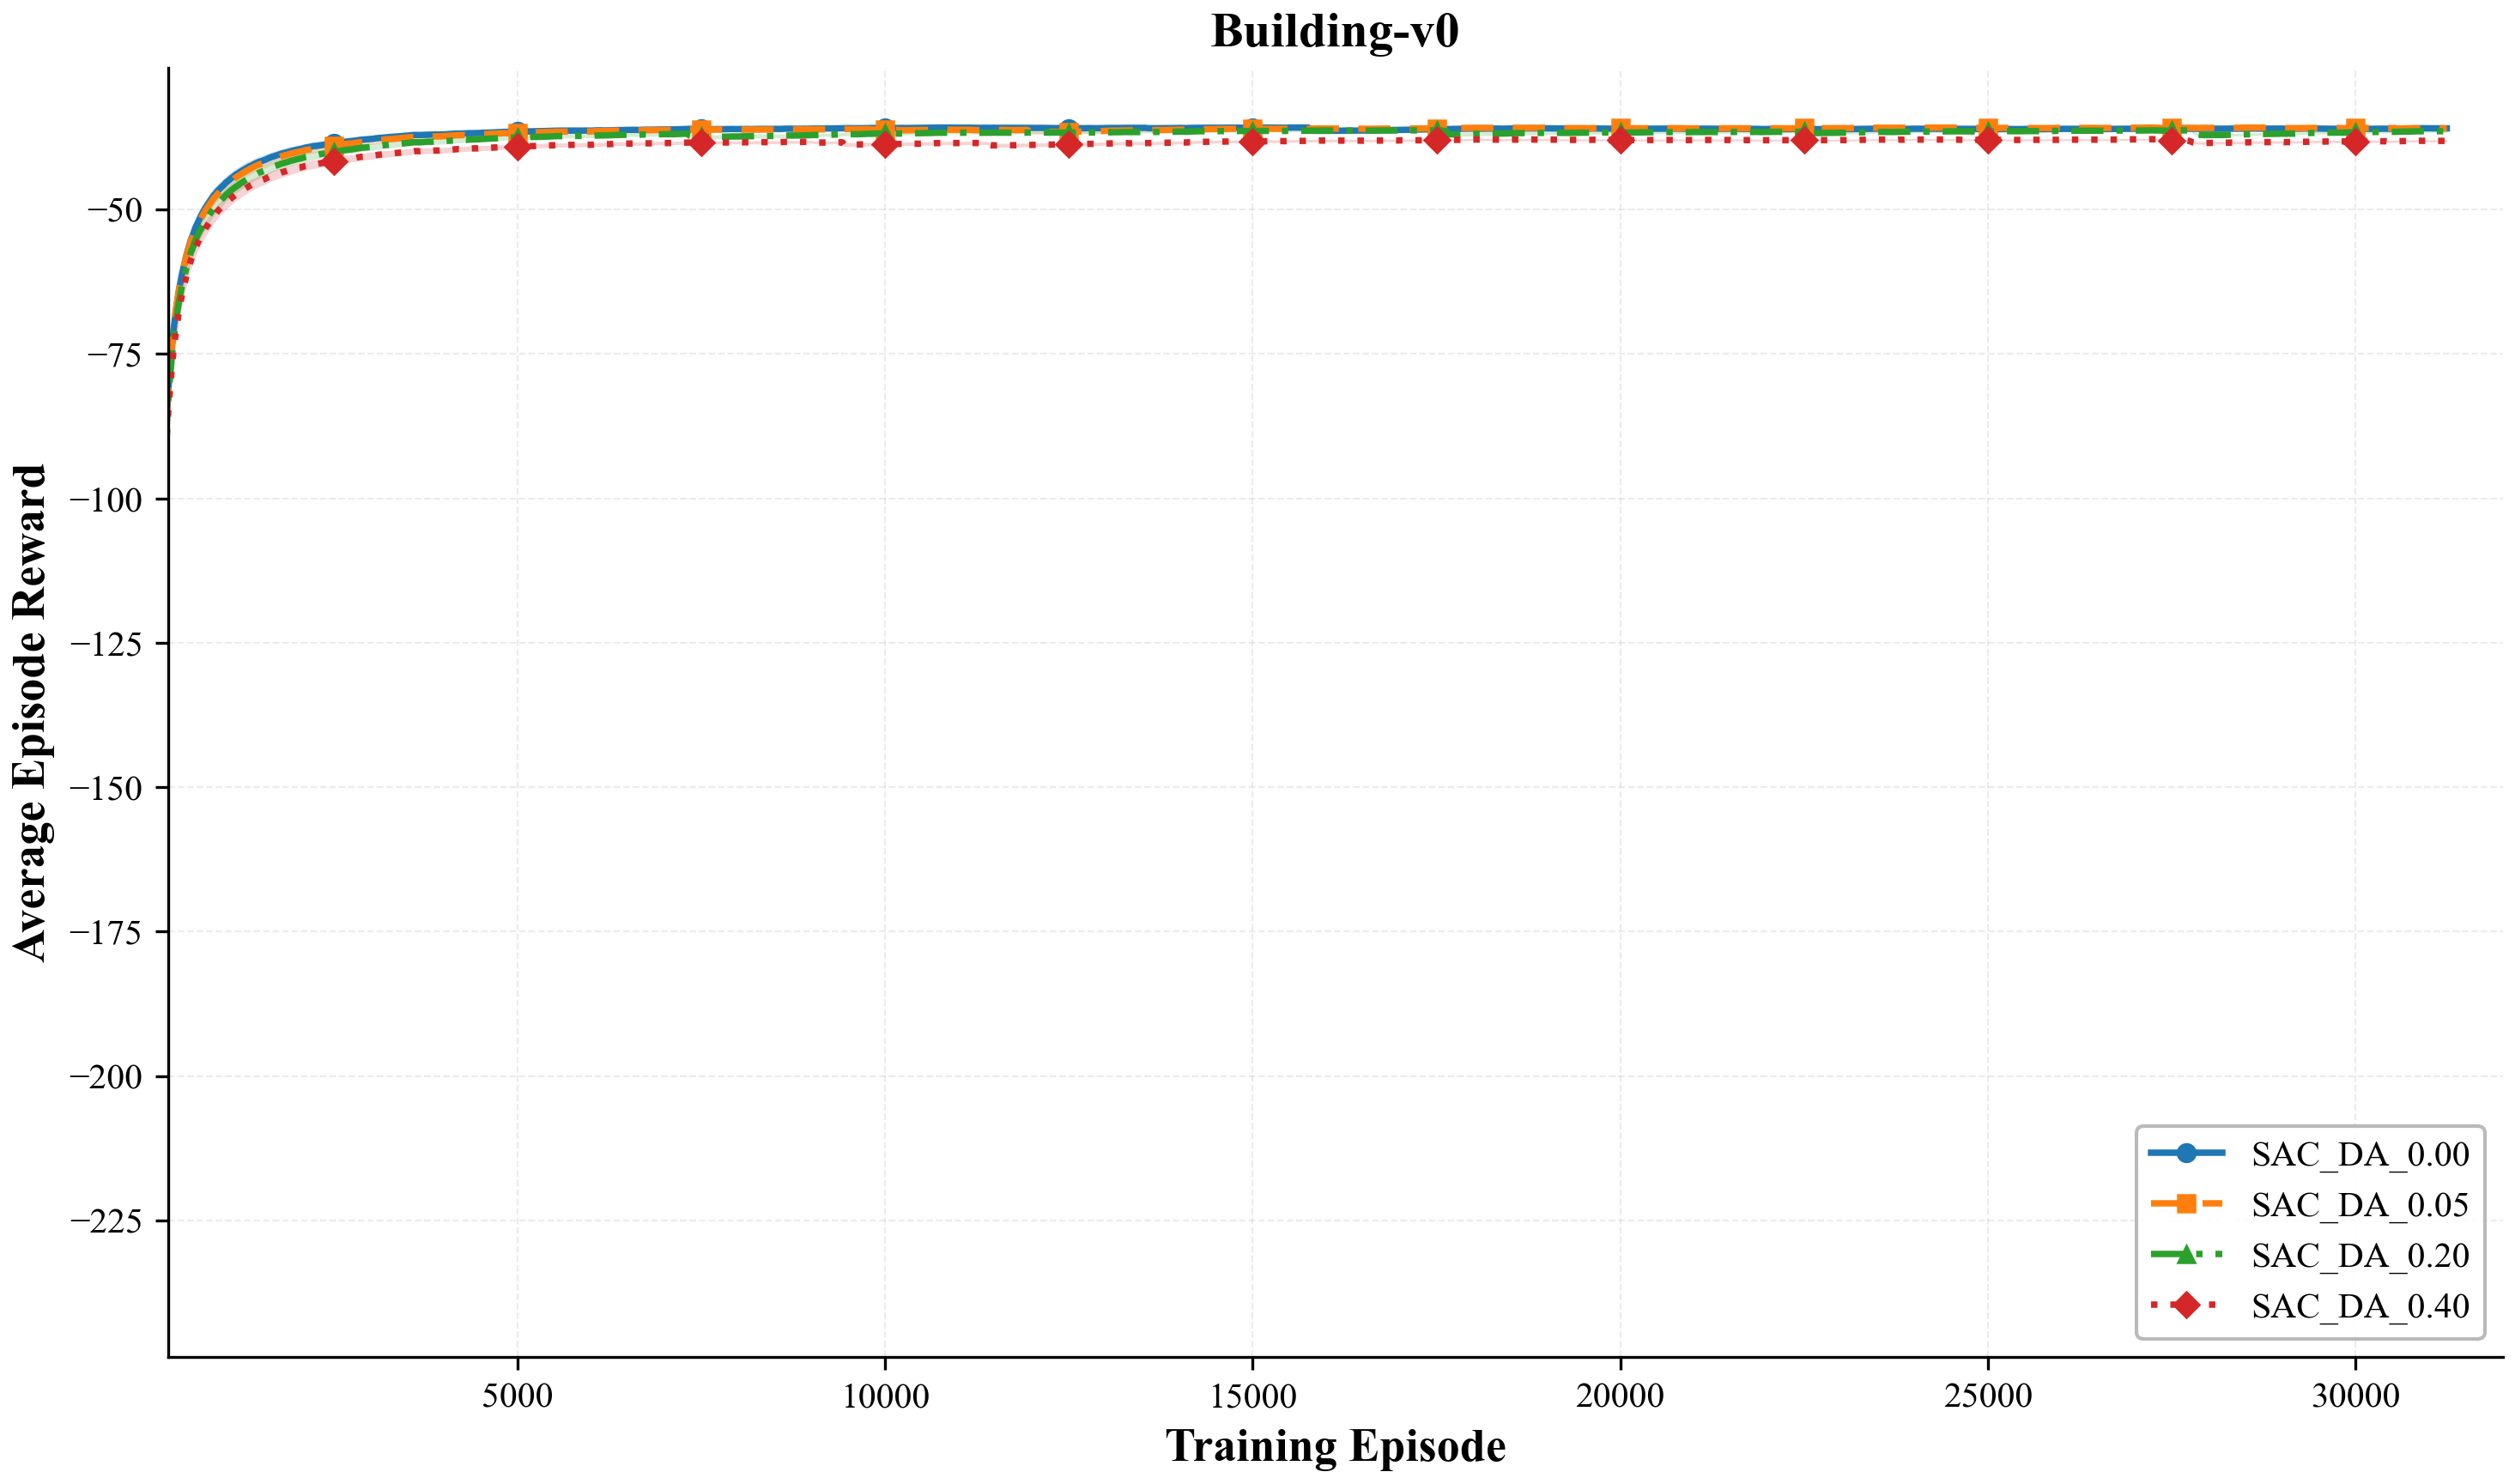
\includegraphics[width=0.9\textwidth]{figures/C_STDRL/bu/SAC/DA_2026-03-16_23-32-25.png}
\caption{Building SAC: Training curves under action noise (DA).}
\label{fig:stdrl_bu_sac_da}
\end{figure}

\begin{figure}[htbp]
\centering
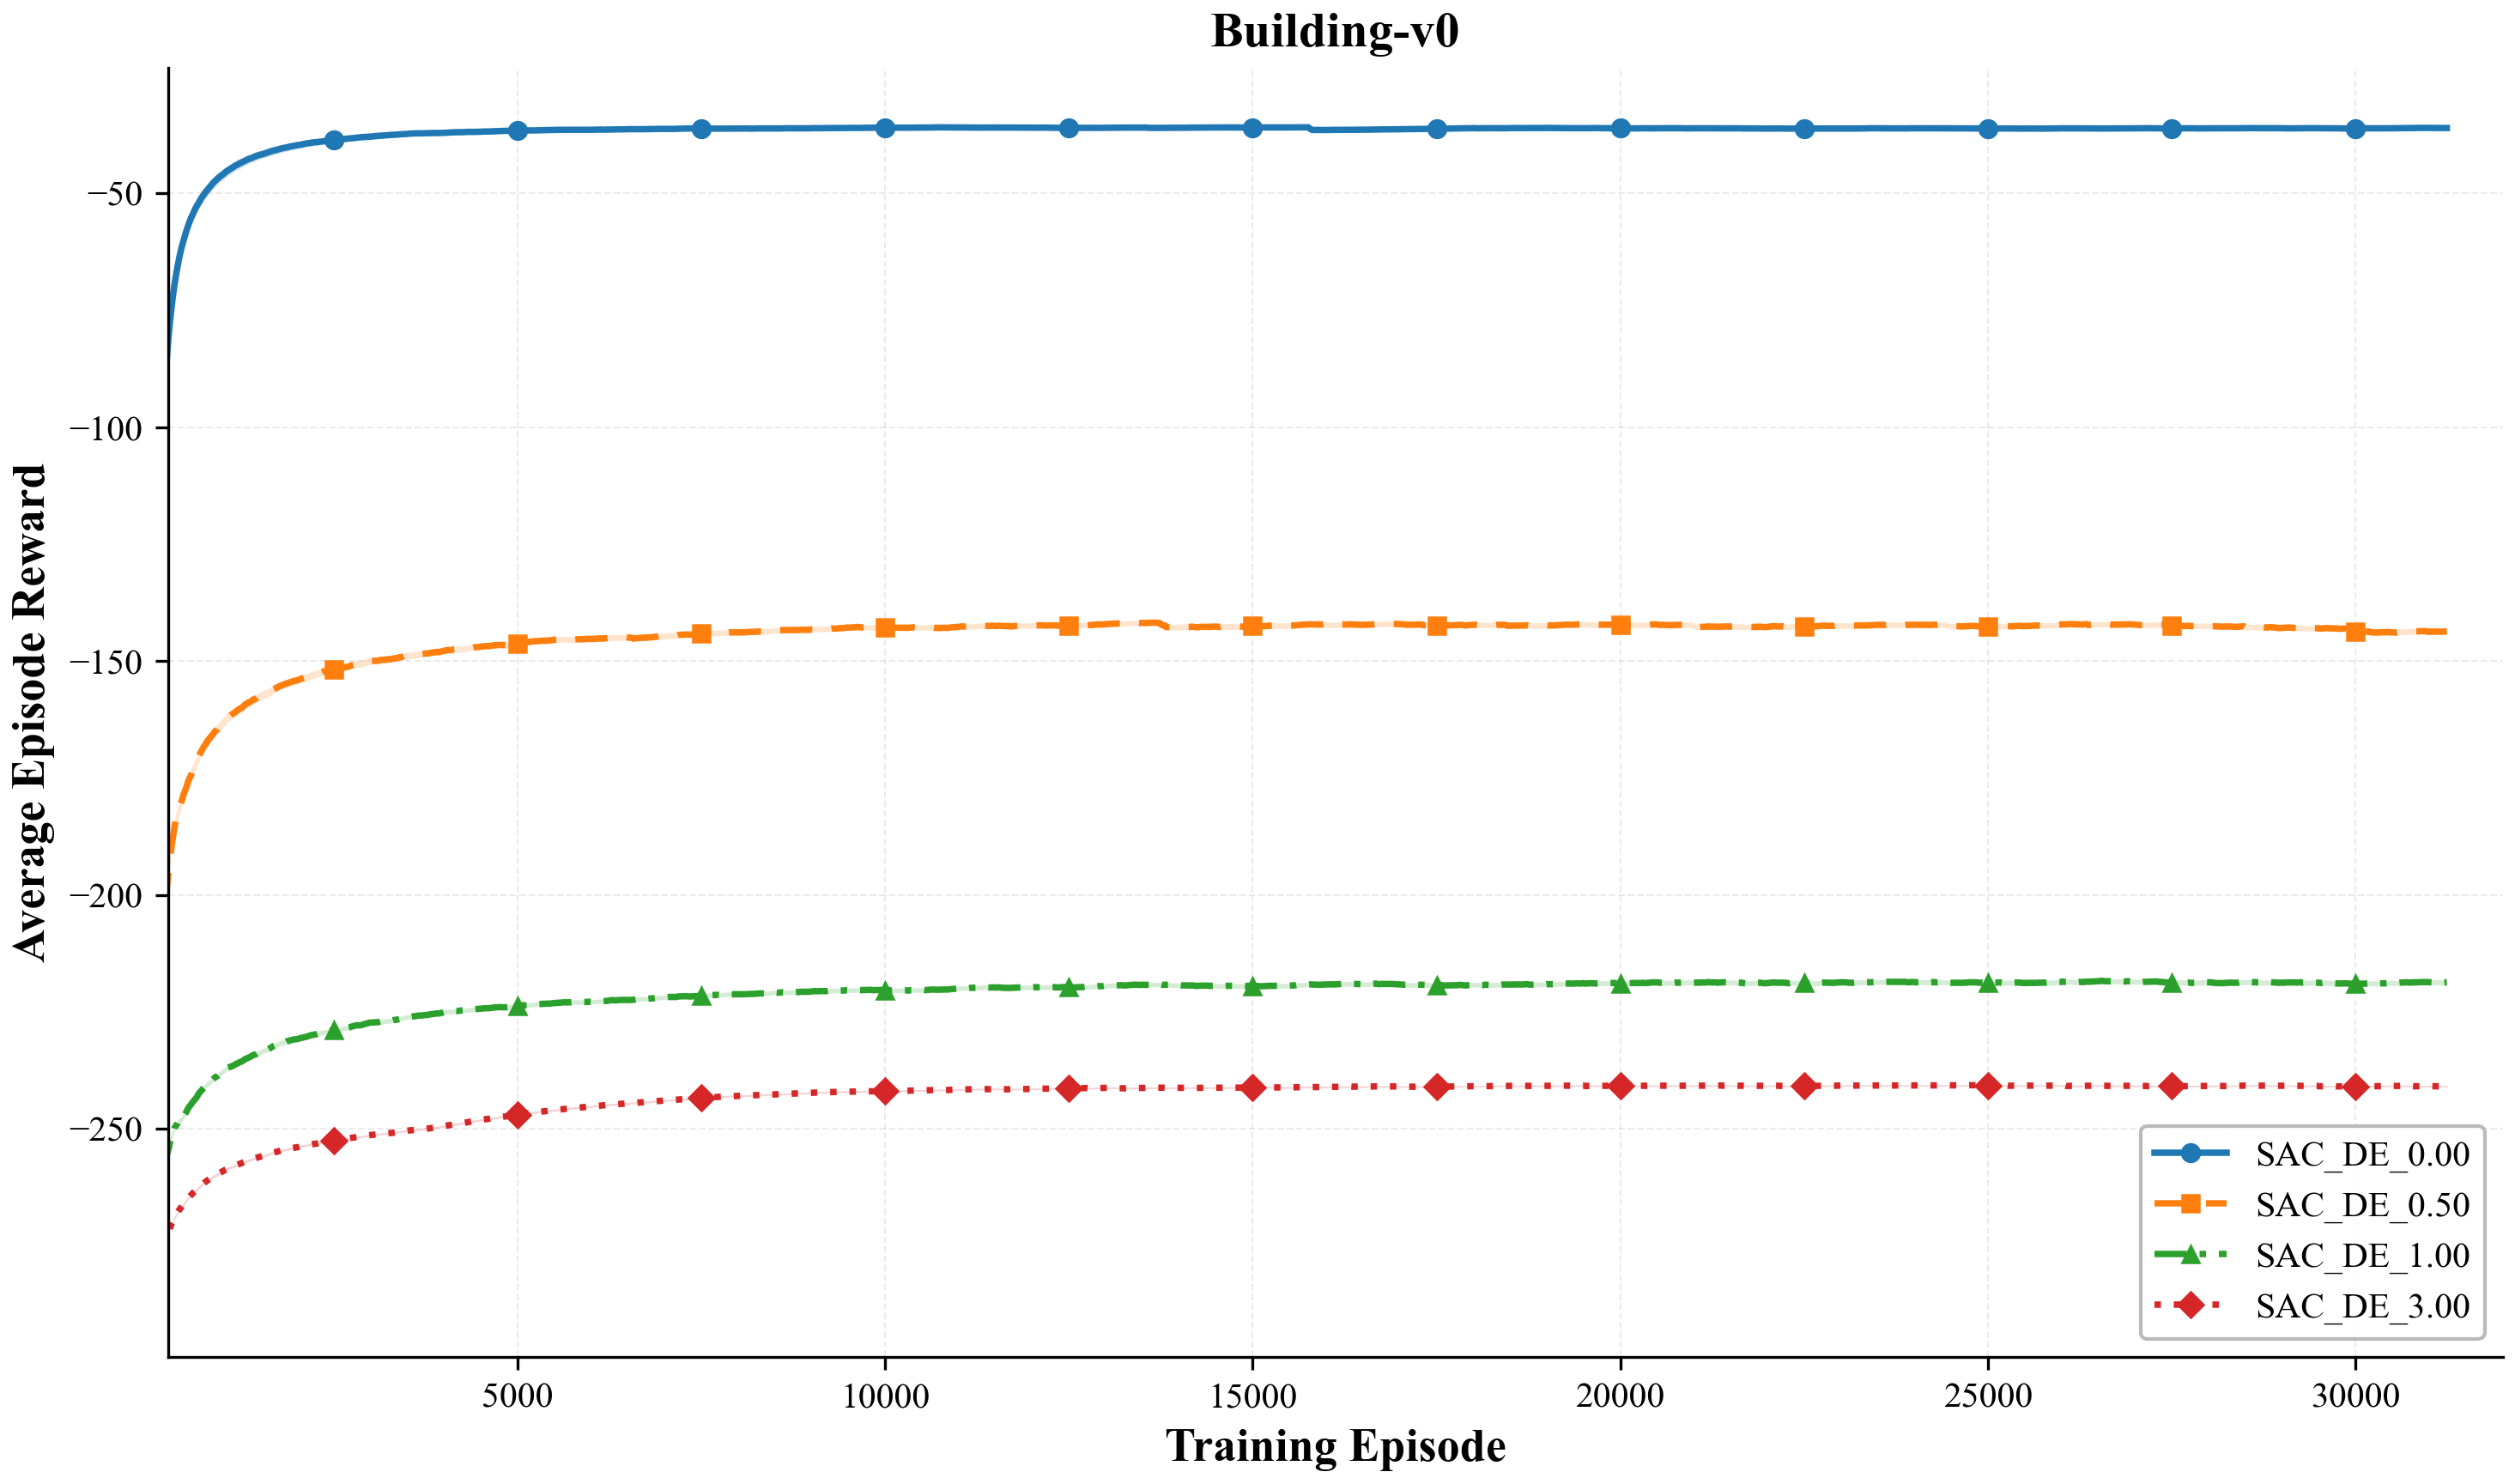
\includegraphics[width=0.9\textwidth]{figures/C_STDRL/bu/SAC/DE_2026-03-16_23-32-27.png}
\caption{Building SAC: Training curves under environment noise (DE).}
\label{fig:stdrl_bu_sac_de}
\end{figure}

\paragraph{Test-time robustness.} SAC's reward distributions (\Cref{fig:violin_bu_sac_obs,fig:violin_bu_sac_act,fig:violin_bu_sac_env}) show similar degradation patterns to PPO, confirming that the Building environment's noise sensitivity is environment-driven rather than algorithm-specific.

\begin{figure}[htbp]
\centering

\includegraphics[width=0.9\textwidth]{figures/C_POST/building/SAC/obs_violin.png}
\caption{Building SAC: Reward distribution under observation noise.}
\label{fig:violin_bu_sac_obs}
\end{figure}

\begin{figure}[htbp]
\centering

\includegraphics[width=0.9\textwidth]{figures/C_POST/building/SAC/action_violin.png}
\caption{Building SAC: Reward distribution under action noise.}
\label{fig:violin_bu_sac_act}
\end{figure}

\begin{figure}[htbp]
\centering

\includegraphics[width=0.9\textwidth]{figures/C_POST/building/SAC/env_violin.png}
\caption{Building SAC: Reward distribution under environment noise.}
\label{fig:violin_bu_sac_env}
\end{figure}

\begin{figure}[htbp]
\centering

\includegraphics[width=0.9\textwidth]{figures/C_POST/building/SAC/panel.png}
\caption{Building SAC: Summary panel across all three noise channels.}
\label{fig:post_bu_sac_panel}
\end{figure}

% ============================================================
\subsection{Cogeneration: Noise Robustness}
\label{sec:noise_co}

The Cogeneration environment reveals a striking algorithm-dependent divergence under noise: PPO is virtually immune to all noise types, while SAC degrades catastrophically under observation noise. This reflects fundamental differences in policy conservatism.

% --- Cogen PPO ---
\subsubsection{Cogeneration --- PPO}

\paragraph{Training curves.} PPO training curves (\Cref{fig:stdrl_co_ppo_ds,fig:stdrl_co_ppo_da,fig:stdrl_co_ppo_de}) are indistinguishable across noise levels, reflecting the conservative fuel-minimizing strategy that inherently tolerates perturbations.

\begin{figure}[htbp]
\centering
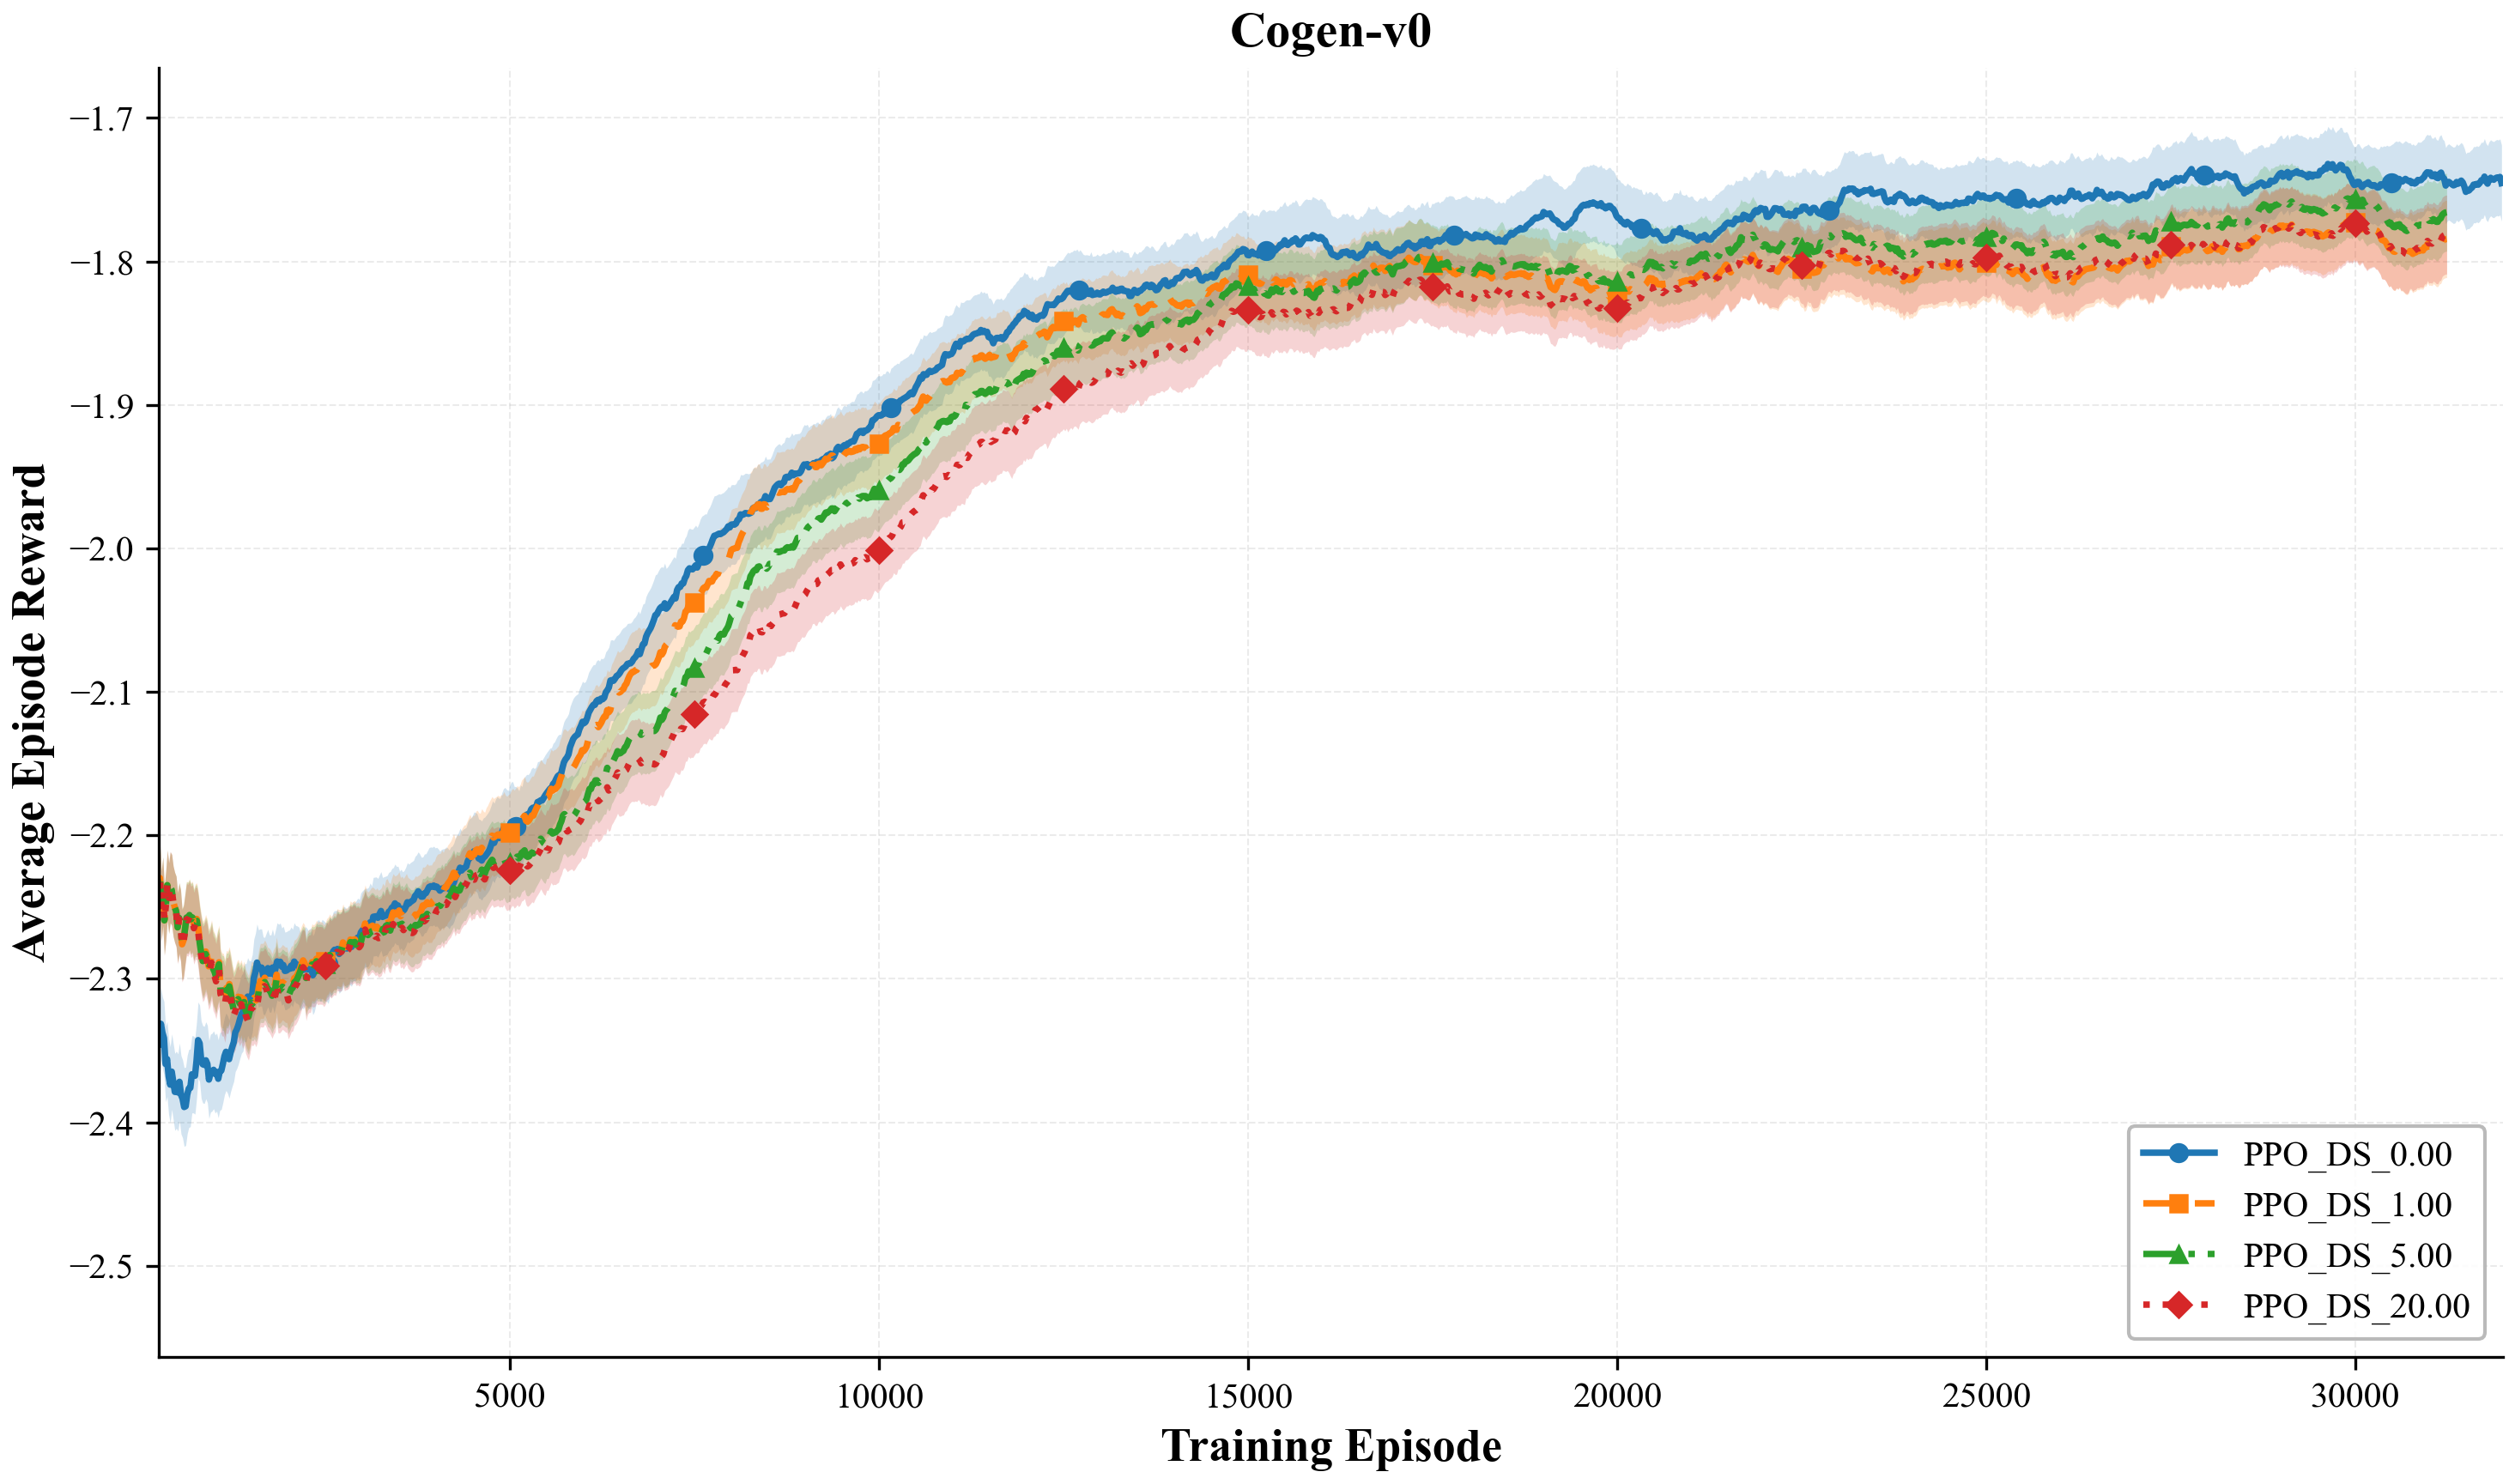
\includegraphics[width=0.9\textwidth]{figures/C_STDRL/co/PPO/DS_2026-03-16_23-32-34.png}
\caption{Cogen PPO: Training curves under observation noise (DS).}
\label{fig:stdrl_co_ppo_ds}
\end{figure}

\begin{figure}[htbp]
\centering
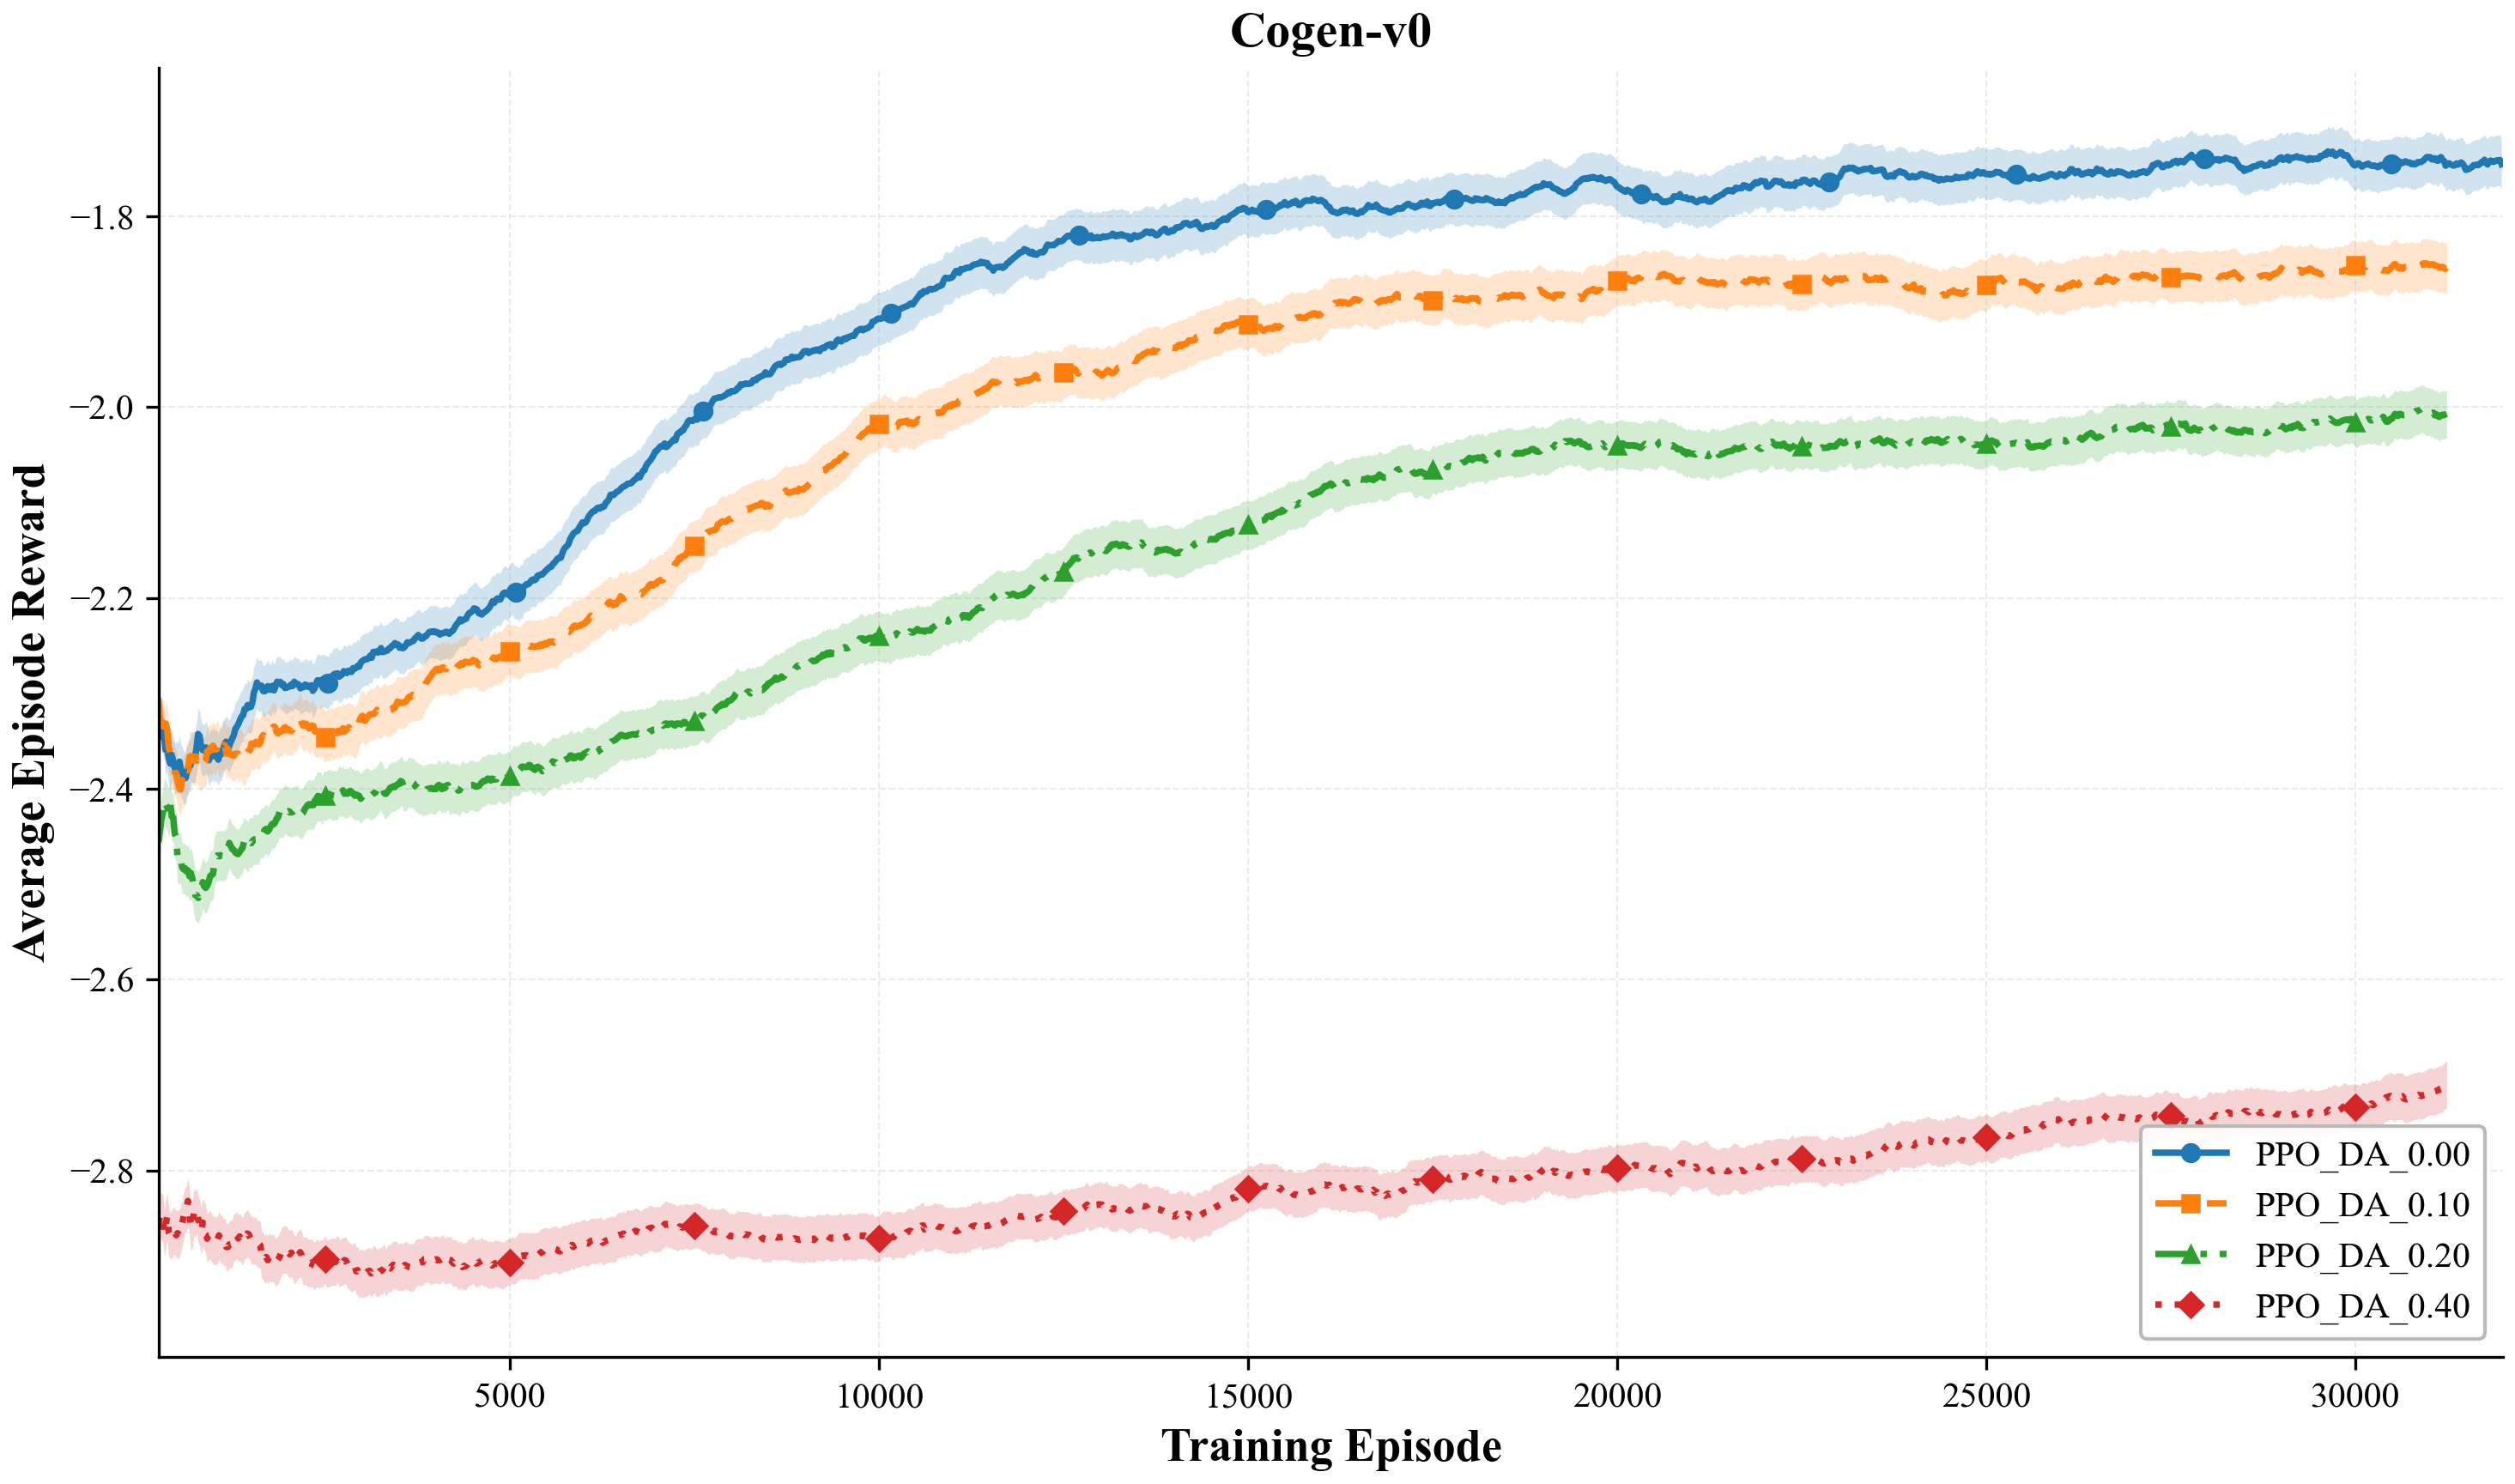
\includegraphics[width=0.9\textwidth]{figures/C_STDRL/co/PPO/DA_2026-03-16_23-32-36.png}
\caption{Cogen PPO: Training curves under action noise (DA).}
\label{fig:stdrl_co_ppo_da}
\end{figure}

\begin{figure}[htbp]
\centering
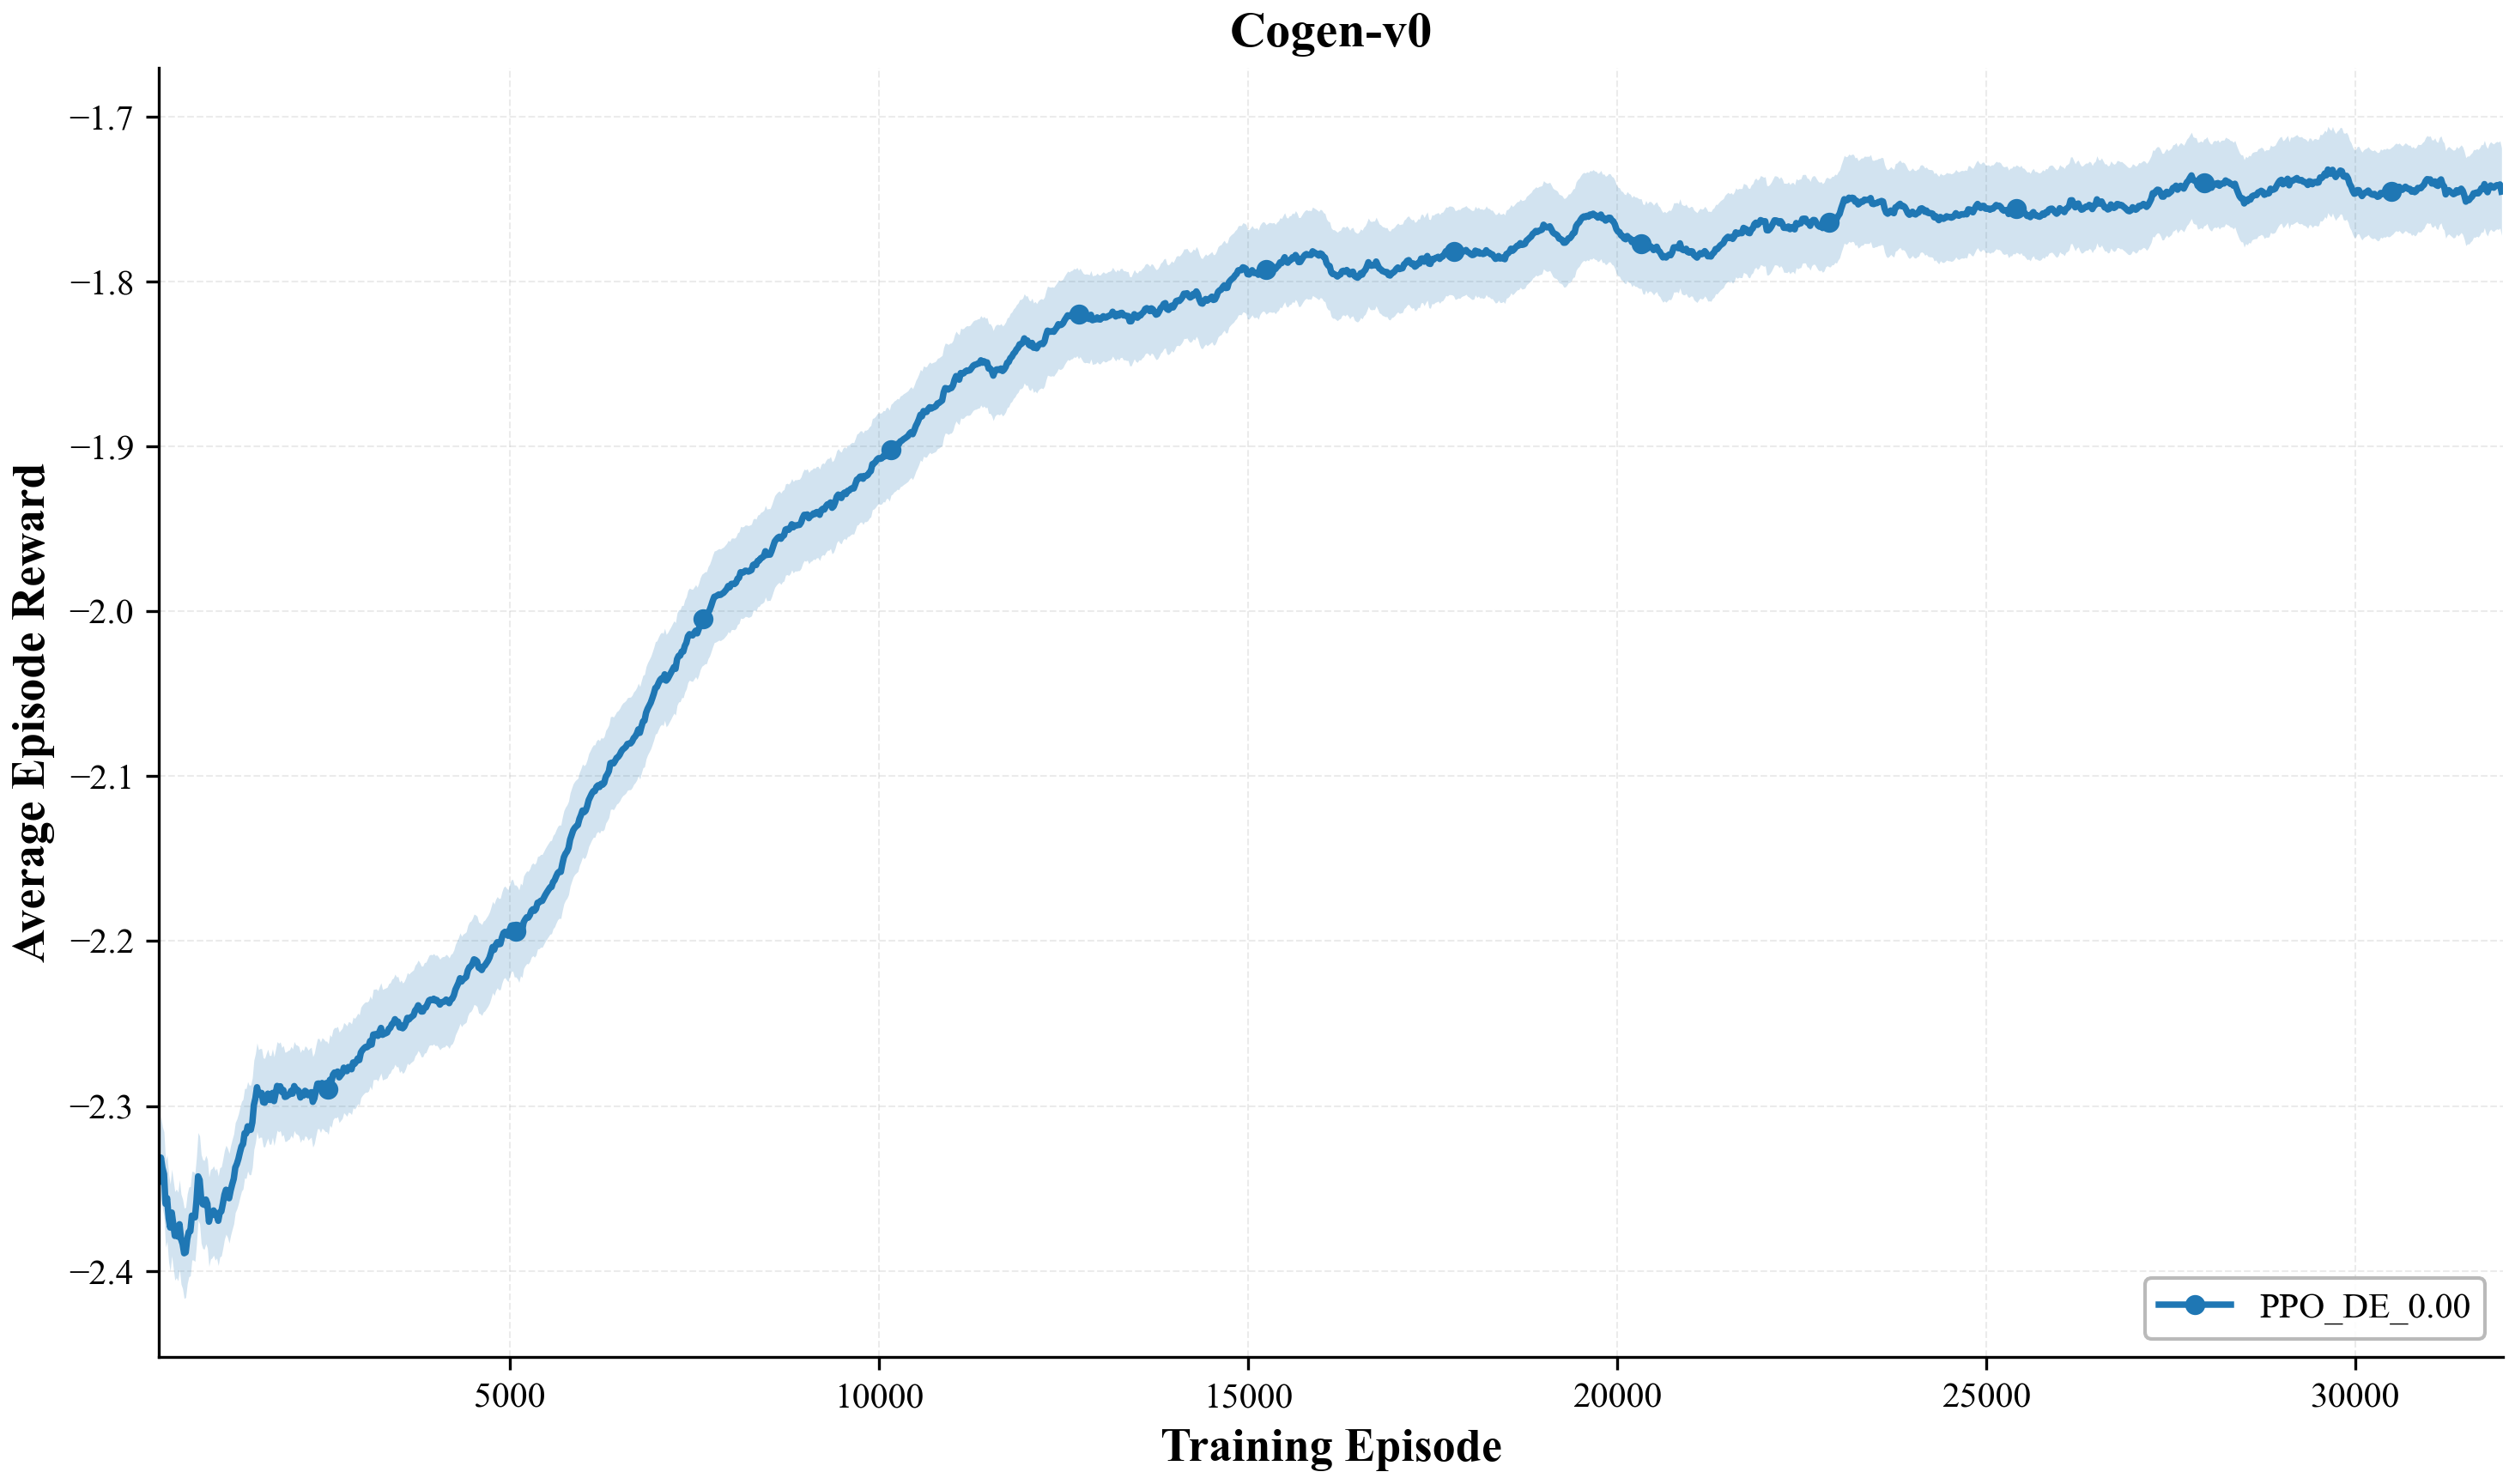
\includegraphics[width=0.9\textwidth]{figures/C_STDRL/co/PPO/DE_2026-03-16_23-32-38.png}
\caption{Cogen PPO: Training curves under environment noise (DE).}
\label{fig:stdrl_co_ppo_de}
\end{figure}

\paragraph{Test-time robustness.} The violin plots (\Cref{fig:violin_co_ppo_obs,fig:violin_co_ppo_act,fig:violin_co_ppo_env}) confirm that PPO's tight reward distribution remains virtually unchanged across the full noise range ($\sigma = 0$ to $5$). Less than $0.3\%$ degradation is observed across all noise channels, reflecting the conservative fuel-minimizing strategy where small actions are inherently insensitive to input perturbations.

\begin{figure}[htbp]
\centering

\includegraphics[width=0.9\textwidth]{figures/C_POST/cogen/PPO/obs_violin.png}
\caption{Cogen PPO: Reward distribution under observation noise. The tight distribution remains unchanged across the full noise range ($\sigma = 0$ to $5$).}
\label{fig:violin_co_ppo_obs}
\end{figure}

\begin{figure}[htbp]
\centering

\includegraphics[width=0.9\textwidth]{figures/C_POST/cogen/PPO/action_violin.png}
\caption{Cogen PPO: Reward distribution under action noise.}
\label{fig:violin_co_ppo_act}
\end{figure}

\begin{figure}[htbp]
\centering

\includegraphics[width=0.9\textwidth]{figures/C_POST/cogen/PPO/env_violin.png}
\caption{Cogen PPO: Reward distribution under environment noise.}
\label{fig:violin_co_ppo_env}
\end{figure}

\begin{figure}[htbp]
\centering

\includegraphics[width=0.9\textwidth]{figures/C_POST/cogen/PPO/panel.png}
\caption{Cogen PPO: Summary panel. Near-zero sensitivity across all noise channels.}
\label{fig:post_co_ppo_panel}
\end{figure}

% --- Cogen SAC ---
\subsubsection{Cogeneration --- SAC}

\paragraph{Training curves.} SAC training curves (\Cref{fig:stdrl_co_sac_ds,fig:stdrl_co_sac_da,fig:stdrl_co_sac_de}) show clear noise sensitivity, particularly under observation noise where convergence is disrupted at higher noise levels.

\begin{figure}[htbp]
\centering
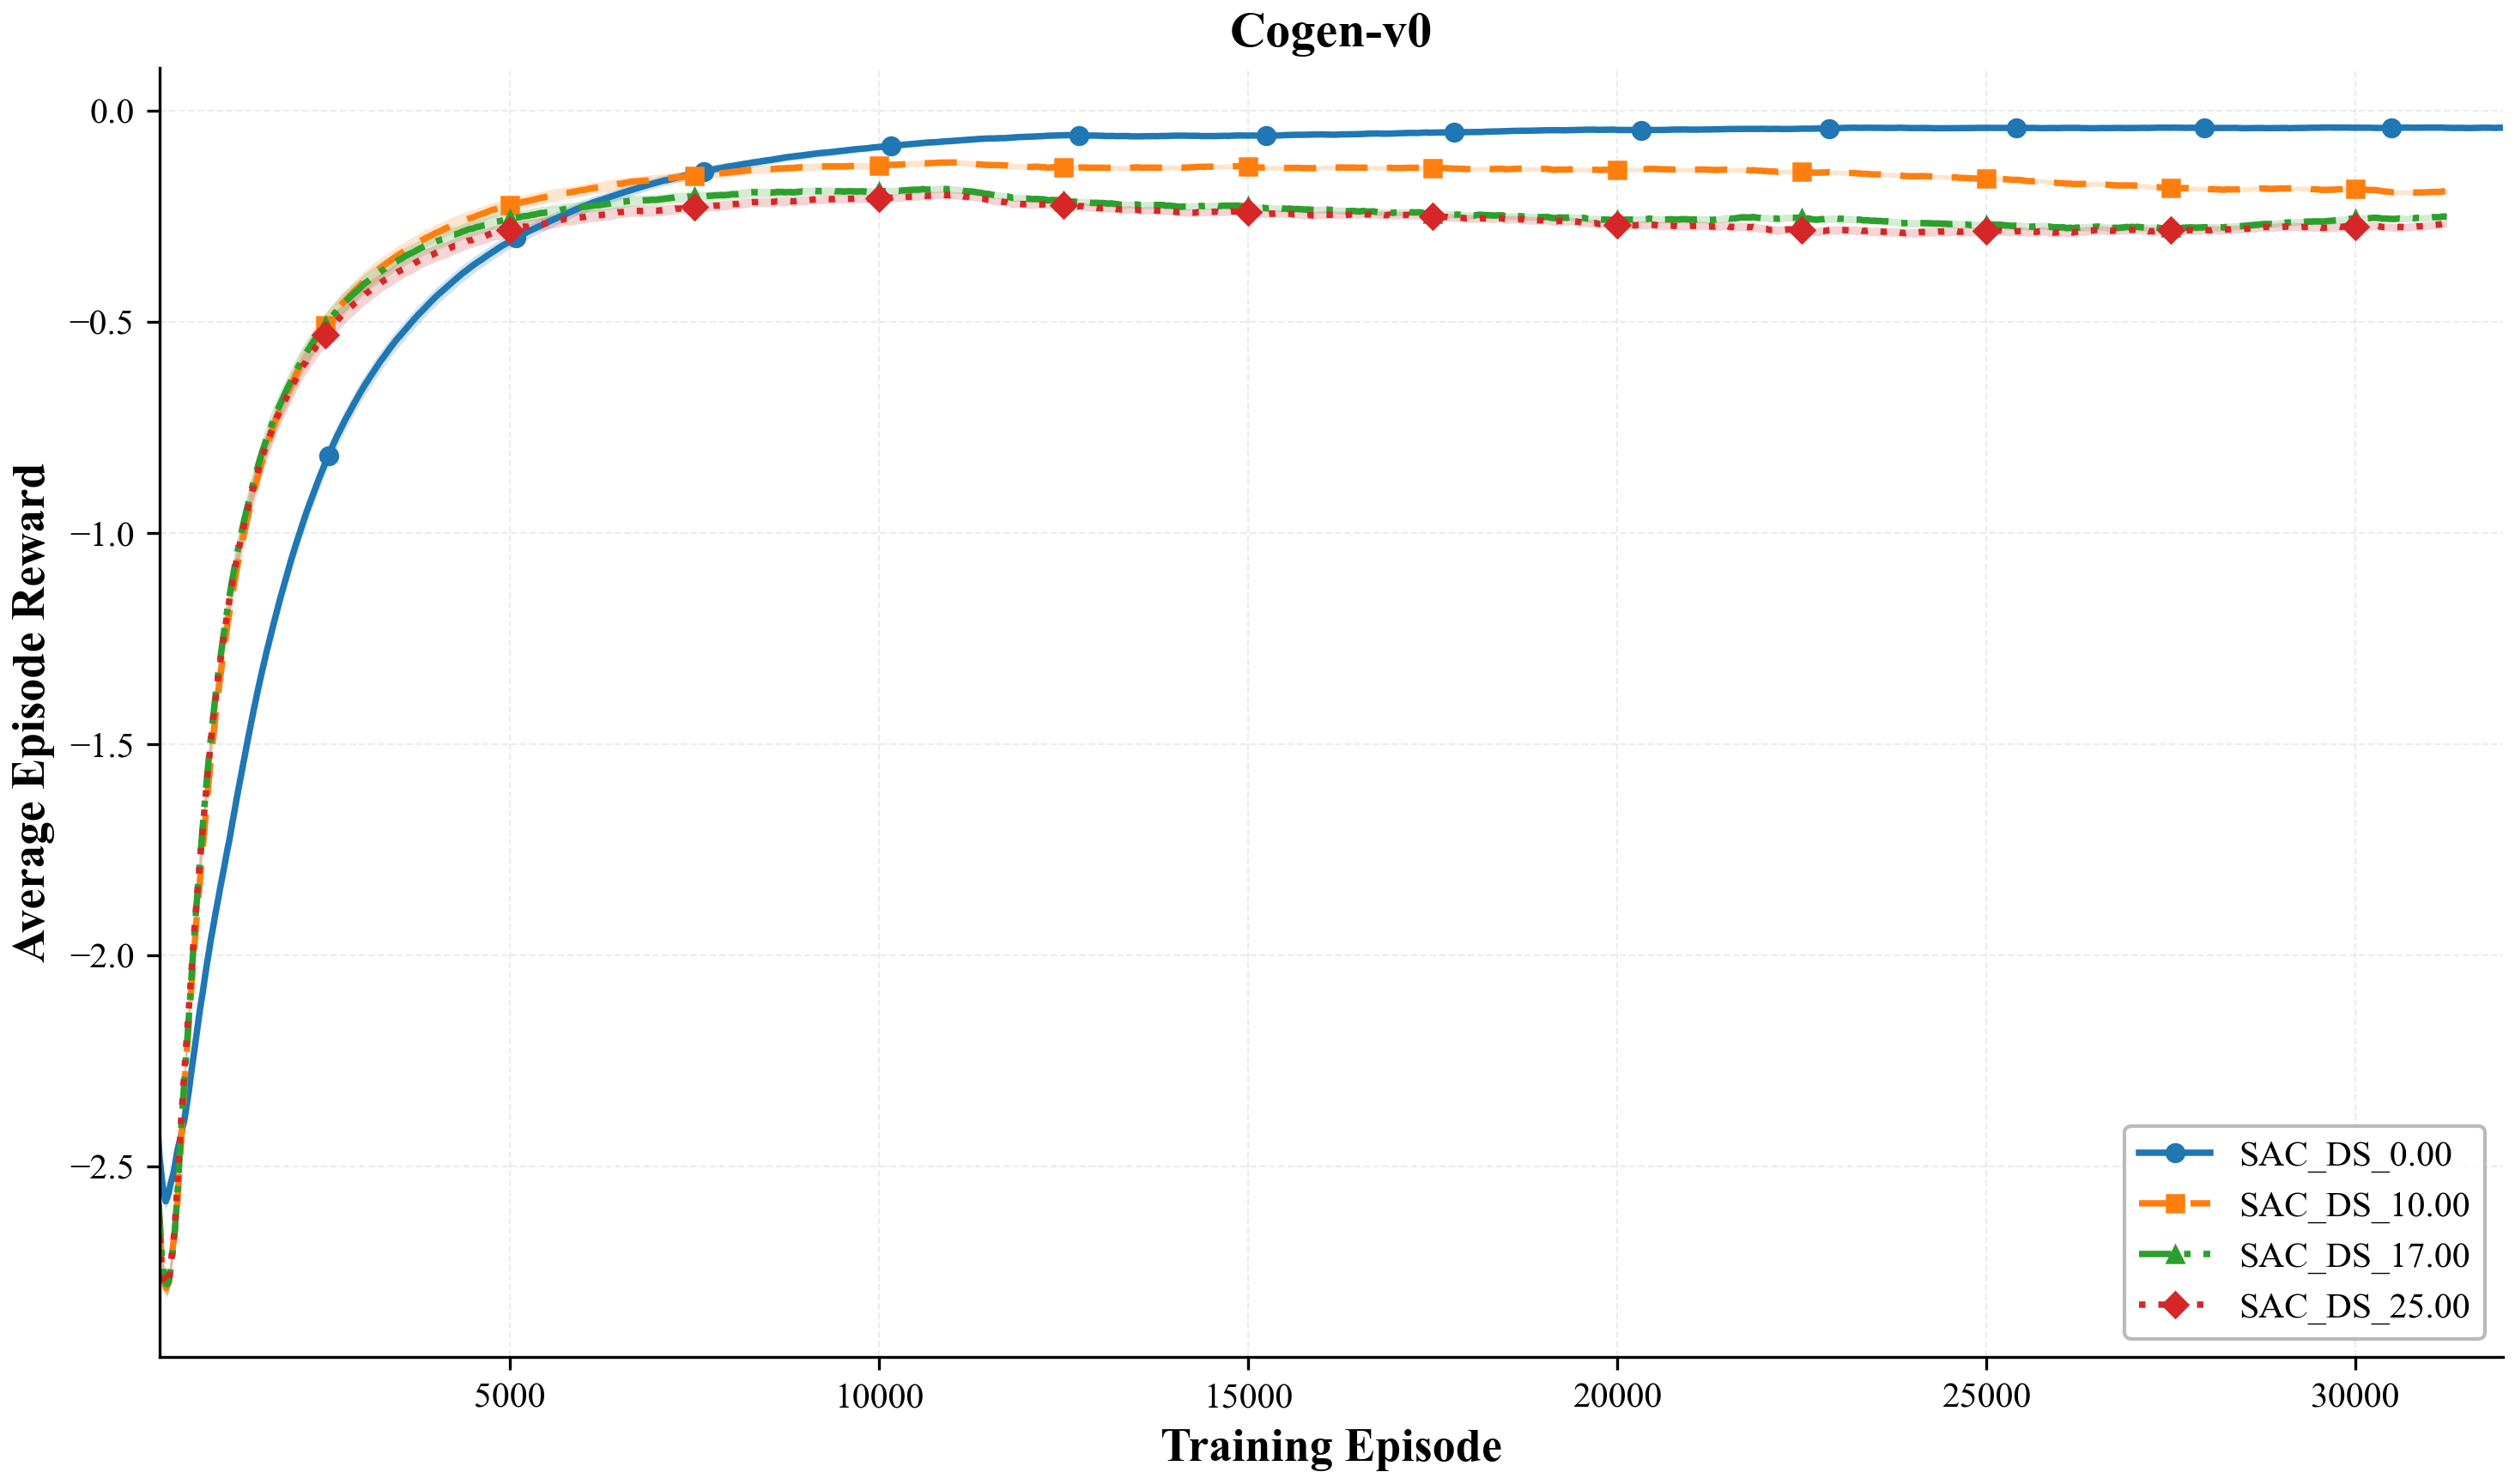
\includegraphics[width=0.9\textwidth]{figures/C_STDRL/co/SAC/DS_2026-03-16_23-32-40.png}
\caption{Cogen SAC: Training curves under observation noise (DS).}
\label{fig:stdrl_co_sac_ds}
\end{figure}

\begin{figure}[htbp]
\centering
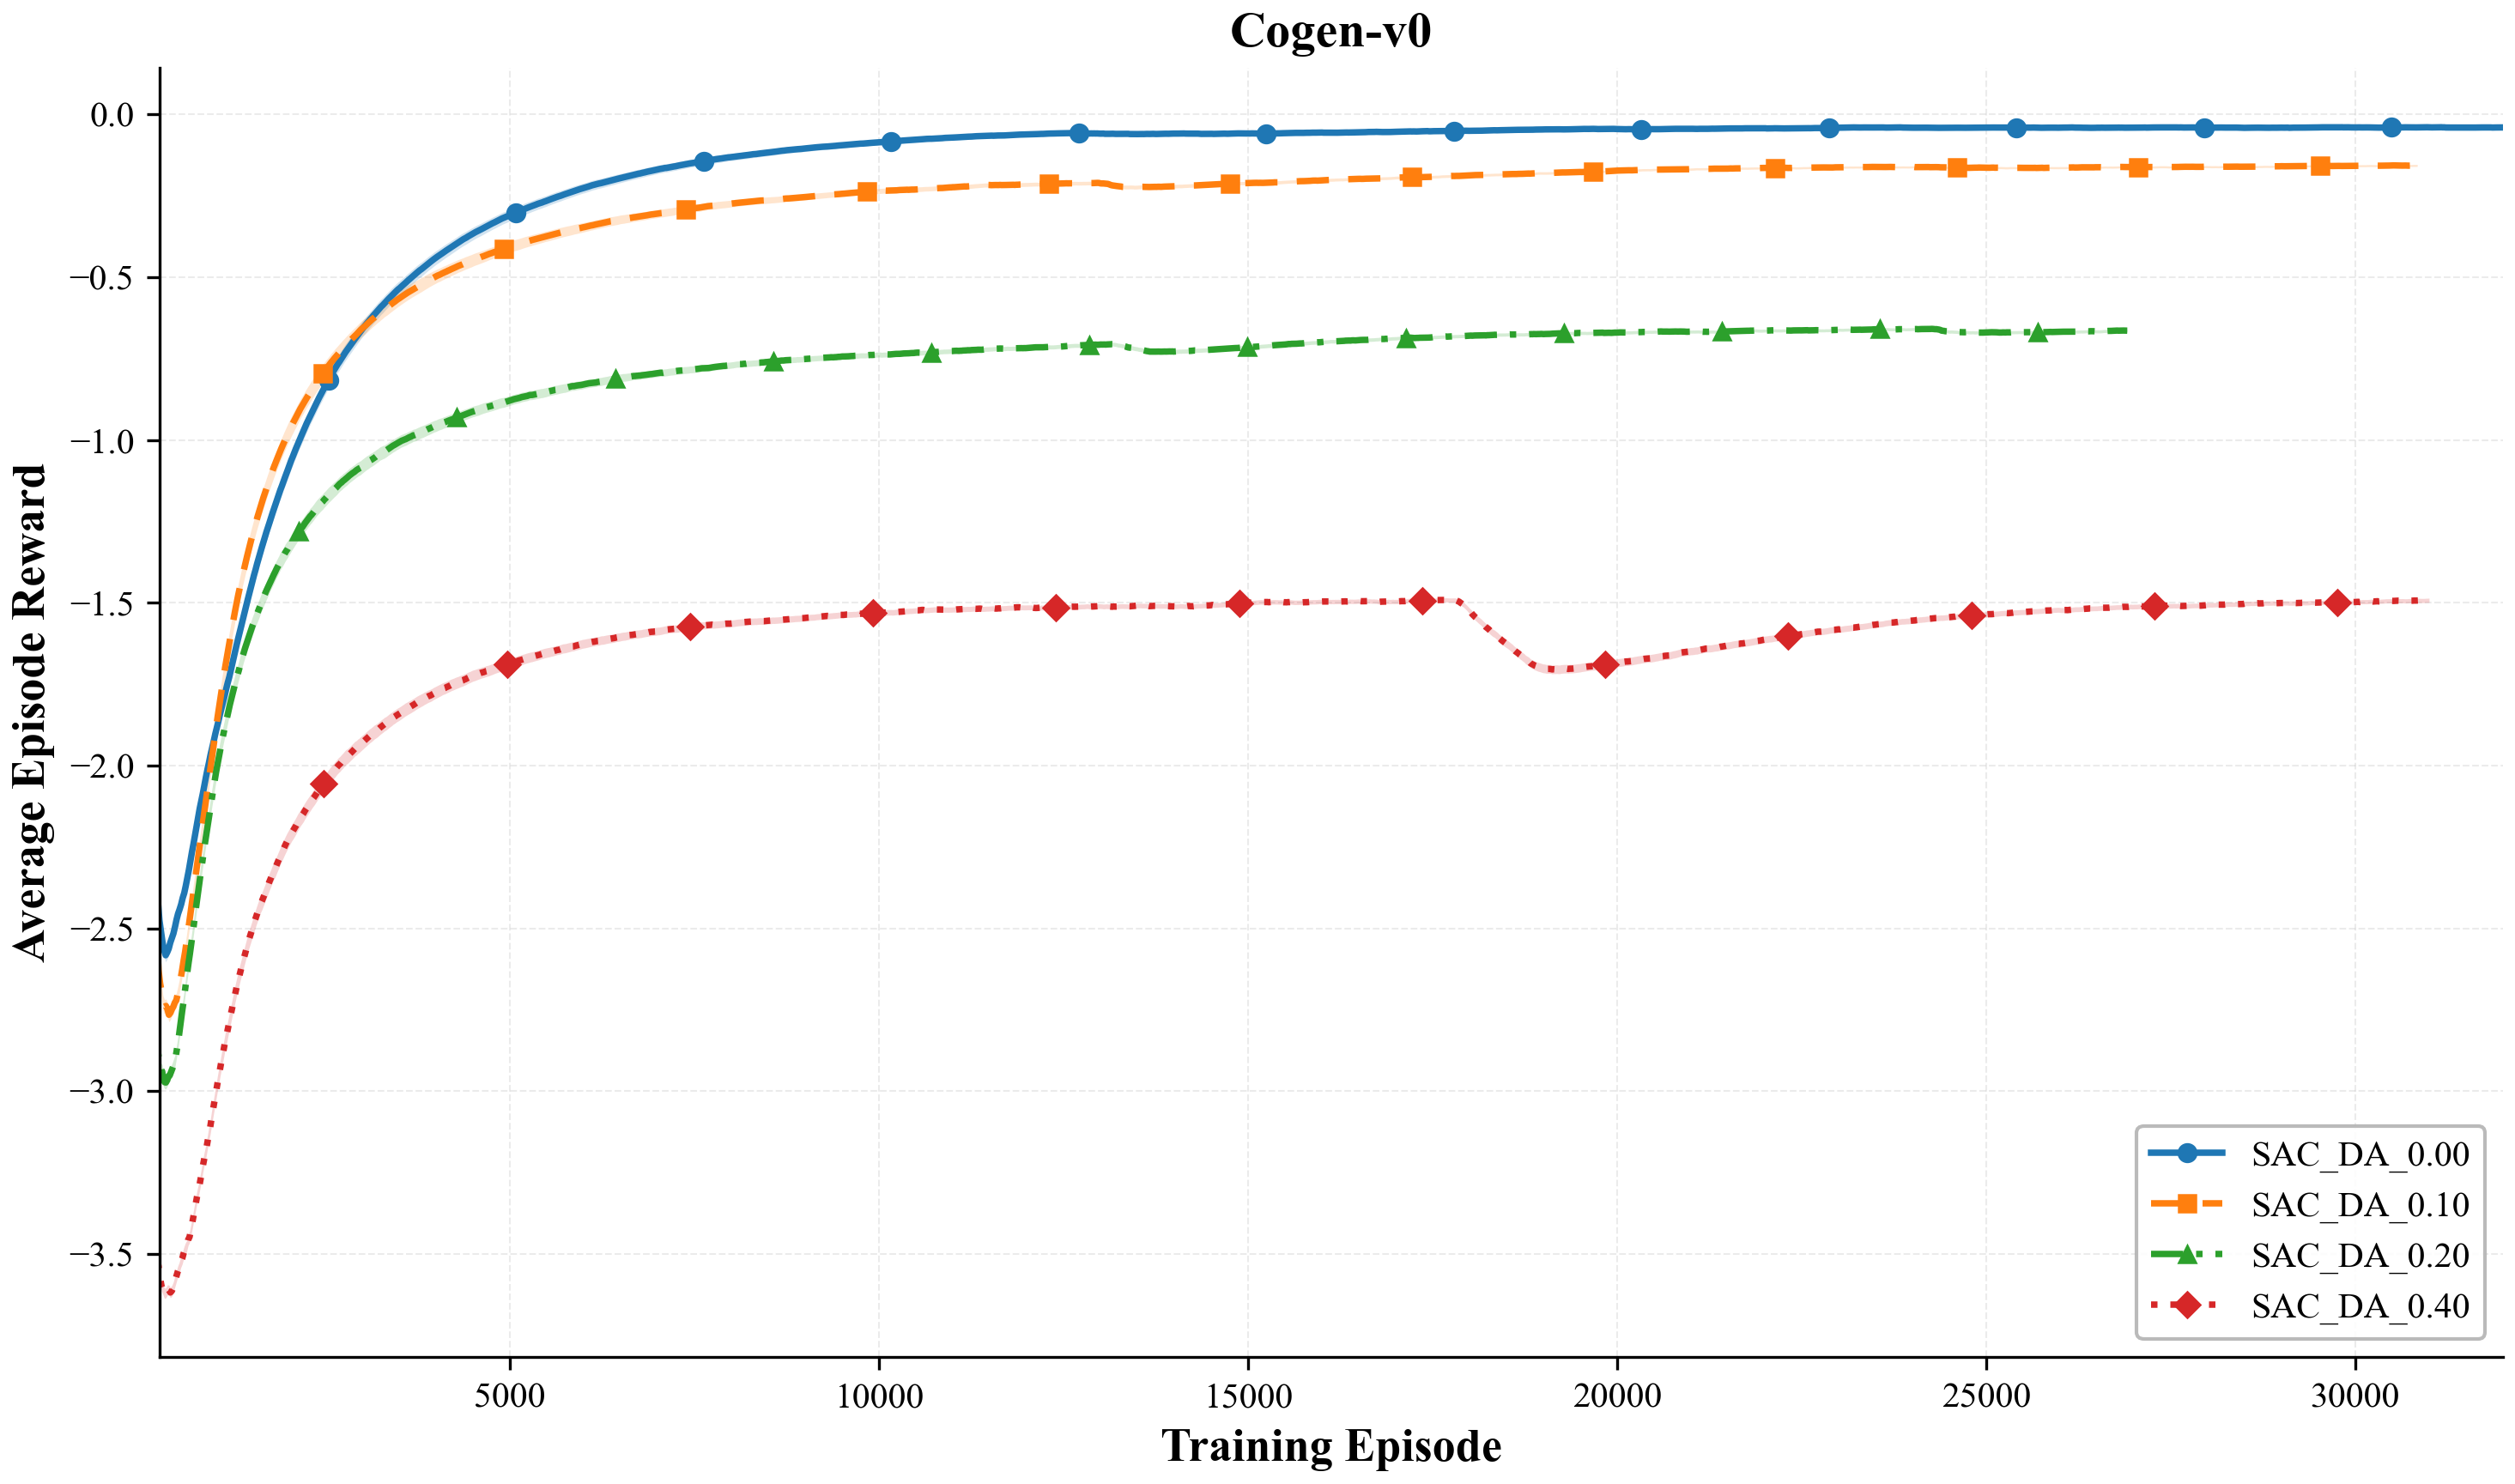
\includegraphics[width=0.9\textwidth]{figures/C_STDRL/co/SAC/DA_2026-03-16_23-32-42.png}
\caption{Cogen SAC: Training curves under action noise (DA).}
\label{fig:stdrl_co_sac_da}
\end{figure}

\begin{figure}[htbp]
\centering
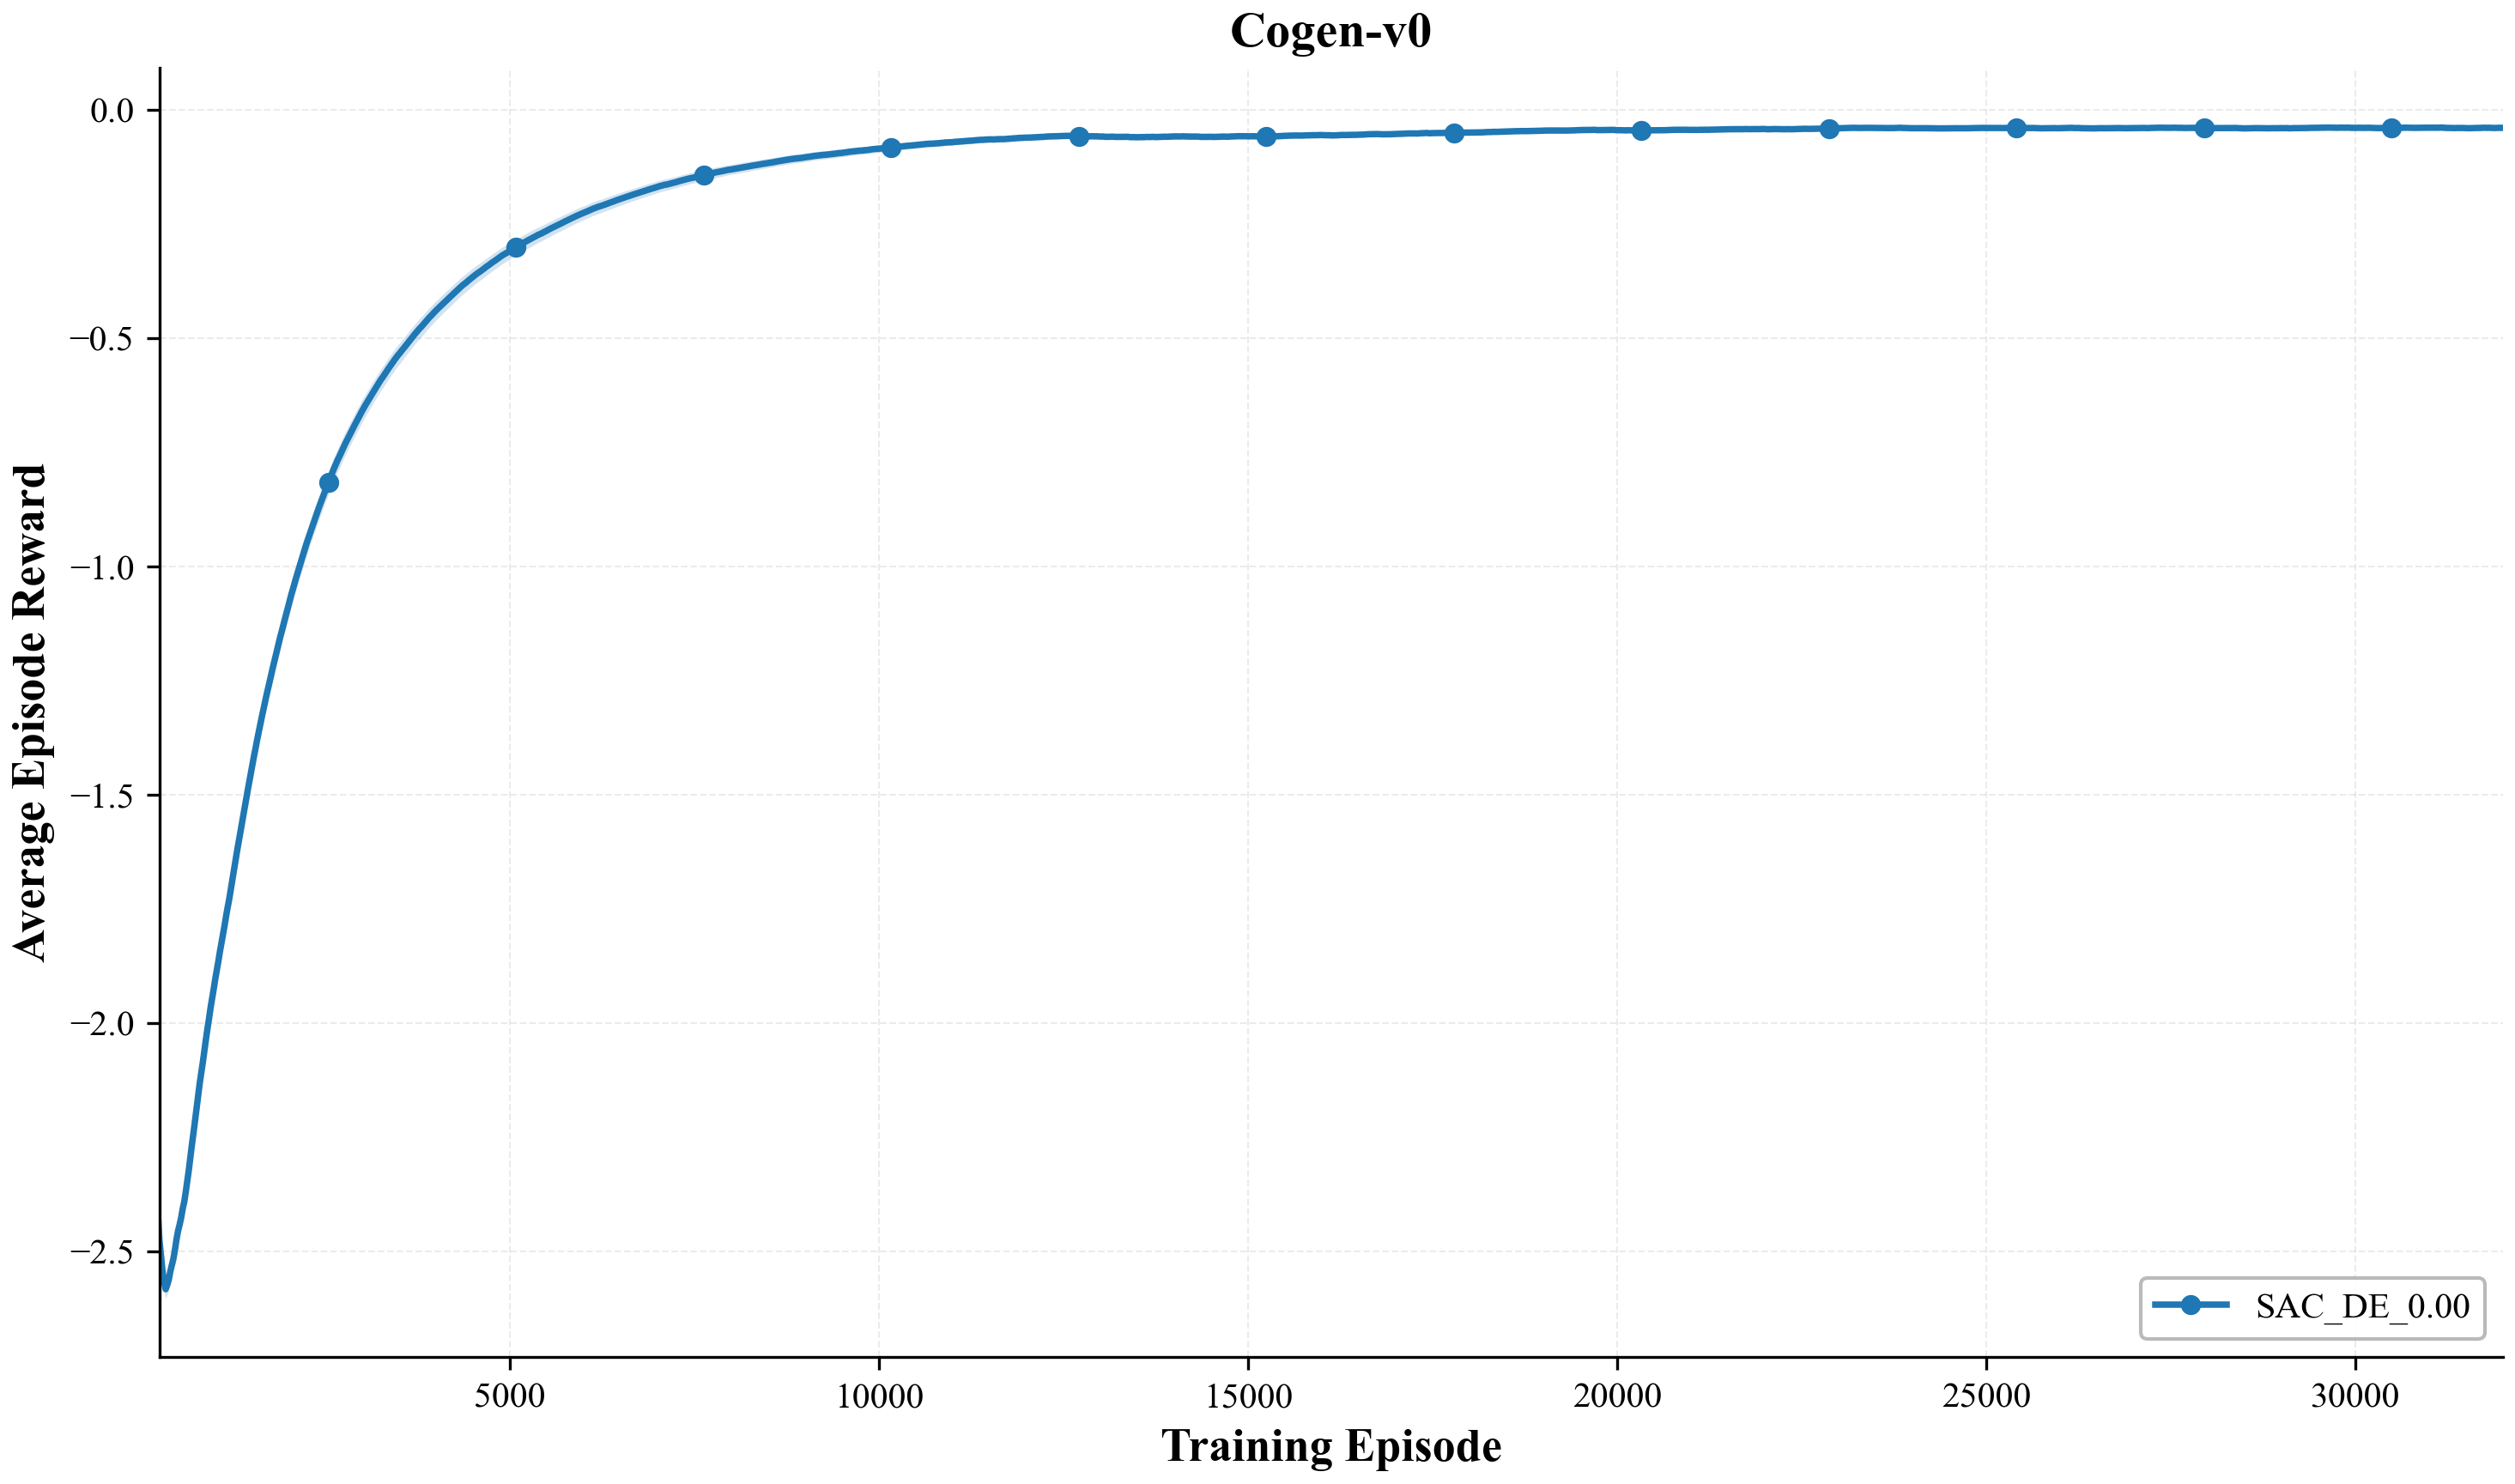
\includegraphics[width=0.9\textwidth]{figures/C_STDRL/co/SAC/DE_2026-03-16_23-32-44.png}
\caption{Cogen SAC: Training curves under environment noise (DE).}
\label{fig:stdrl_co_sac_de}
\end{figure}

\paragraph{Test-time robustness.} SAC's observation noise violin plot (\Cref{fig:violin_co_sac_obs}) shows dramatic degradation: the distribution broadens and shifts leftward, with heavy left tails emerging at $\sigma \geq 2$ indicating frequent constraint violations. SAC's aggressive optimization near the constraint boundary is fragile to observation perturbations. Environment noise (\Cref{fig:violin_co_sac_env}) causes moderate degradation through ONNX model output perturbations.

\begin{figure}[htbp]
\centering

\includegraphics[width=0.9\textwidth]{figures/C_POST/cogen/SAC/obs_violin.png}
\caption{Cogen SAC: Reward distribution under observation noise. Heavy left tails emerge at $\sigma \geq 2$, indicating constraint violations from aggressive near-boundary optimization.}
\label{fig:violin_co_sac_obs}
\end{figure}

\begin{figure}[htbp]
\centering

\includegraphics[width=0.9\textwidth]{figures/C_POST/cogen/SAC/env_violin.png}
\caption{Cogen SAC: Reward distribution under environment noise. ONNX model output perturbations cause moderate degradation with increasing tail weight.}
\label{fig:violin_co_sac_env}
\end{figure}

\begin{figure}[htbp]
\centering

\includegraphics[width=0.9\textwidth]{figures/C_POST/cogen/SAC/panel.png}
\caption{Cogen SAC: Summary panel. Observation noise causes severe degradation; environment noise has moderate impact.}
\label{fig:post_co_sac_panel}
\end{figure}

% ============================================================
\subsection{Noise Robustness Findings}
\label{sec:noise_findings}

\begin{finding}[Environment-Dependent Noise Sensitivity (RQ1, RQ6)]
\label{find:noise_sensitivity}
Noise robustness varies dramatically across environments: EV Charging policies are exceptionally robust to all noise types ($<1\%$ degradation at moderate noise), while Building policies degrade rapidly under observation and environment noise ($>100\%$ degradation at $\sigma \geq 0.15$). This reflects fundamental differences in environment dynamics: EV Charging's reward depends primarily on aggregate daily charging patterns that are noise-resistant, while Building's RC thermal model amplifies per-timestep observation errors through coupled zone dynamics.
\end{finding}

\begin{finding}[Observation vs.\ Action Noise Asymmetry (RQ2)]
\label{find:obs_act_asymmetry}
Across all environments, observation noise causes significantly more degradation than action noise at equivalent scales. The practical implication is clear: for real-world deployment of RL-based controllers, sensor accuracy is more critical than actuator precision.
\end{finding}

\begin{finding}[Algorithm-Specific Robustness (RQ1)]
\label{find:algo_robustness}
PPO consistently demonstrates superior noise robustness compared to SAC and TD3, with the most dramatic difference in Cogeneration (PPO: $<0.3\%$ degradation; SAC: $>2000\%$ degradation). PPO's on-policy training and clipped surrogate objective create naturally conservative policies that tolerate input perturbations, while SAC's entropy-maximizing exploration can amplify noise in the policy output.
\end{finding}

% ============================================================
\section{Safe Reinforcement Learning}
\label{sec:results_saferl}

We evaluate four on-policy CMDP algorithms---PPO-Lagrangian (PPOLag), CPO, OnCRPO, and FOCOPS---under varying cost limits using the CMDP formulations described in \Cref{sec:safe_rl}. All models are trained for 6M steps (3000 epochs $\times$ 2000 steps/epoch) using the OmniSafe framework~\citep{ji2023omnisafe} with the hyperparameters specified in \Cref{sec:experimental_design}.

% ------------------------------------------------------------
\subsection{Cogeneration: Strong Constraint Differentiation}
\label{sec:saferl_cogen}

The Cogeneration environment provides the strongest Safe RL results. The CMDP cost---cumulative turbine ramping stress---is orthogonal to the reward, which is dominated by fuel and delivery costs. The reward's built-in ramp penalty ($w_{\text{ramp}} = 2$) is negligible, so the unconstrained agent ignores turbine stress.

% --- Cogen PPOLag ---
\subsubsection{Cogeneration --- PPOLag}

PPOLag achieves the clearest cost limit differentiation (\Cref{fig:cogen_ppolag}): final episode costs of $5$, $12$, $23$, and $43$ for $d = 10, 25, 50, 200$ respectively---a monotonically increasing sequence. The tightest limit ($d=10$) incurs a reward penalty of $-0.30$ compared to $-0.04$ for loose limits, quantifying the economic cost of smooth turbine operation.

\begin{figure}[htbp]
\centering
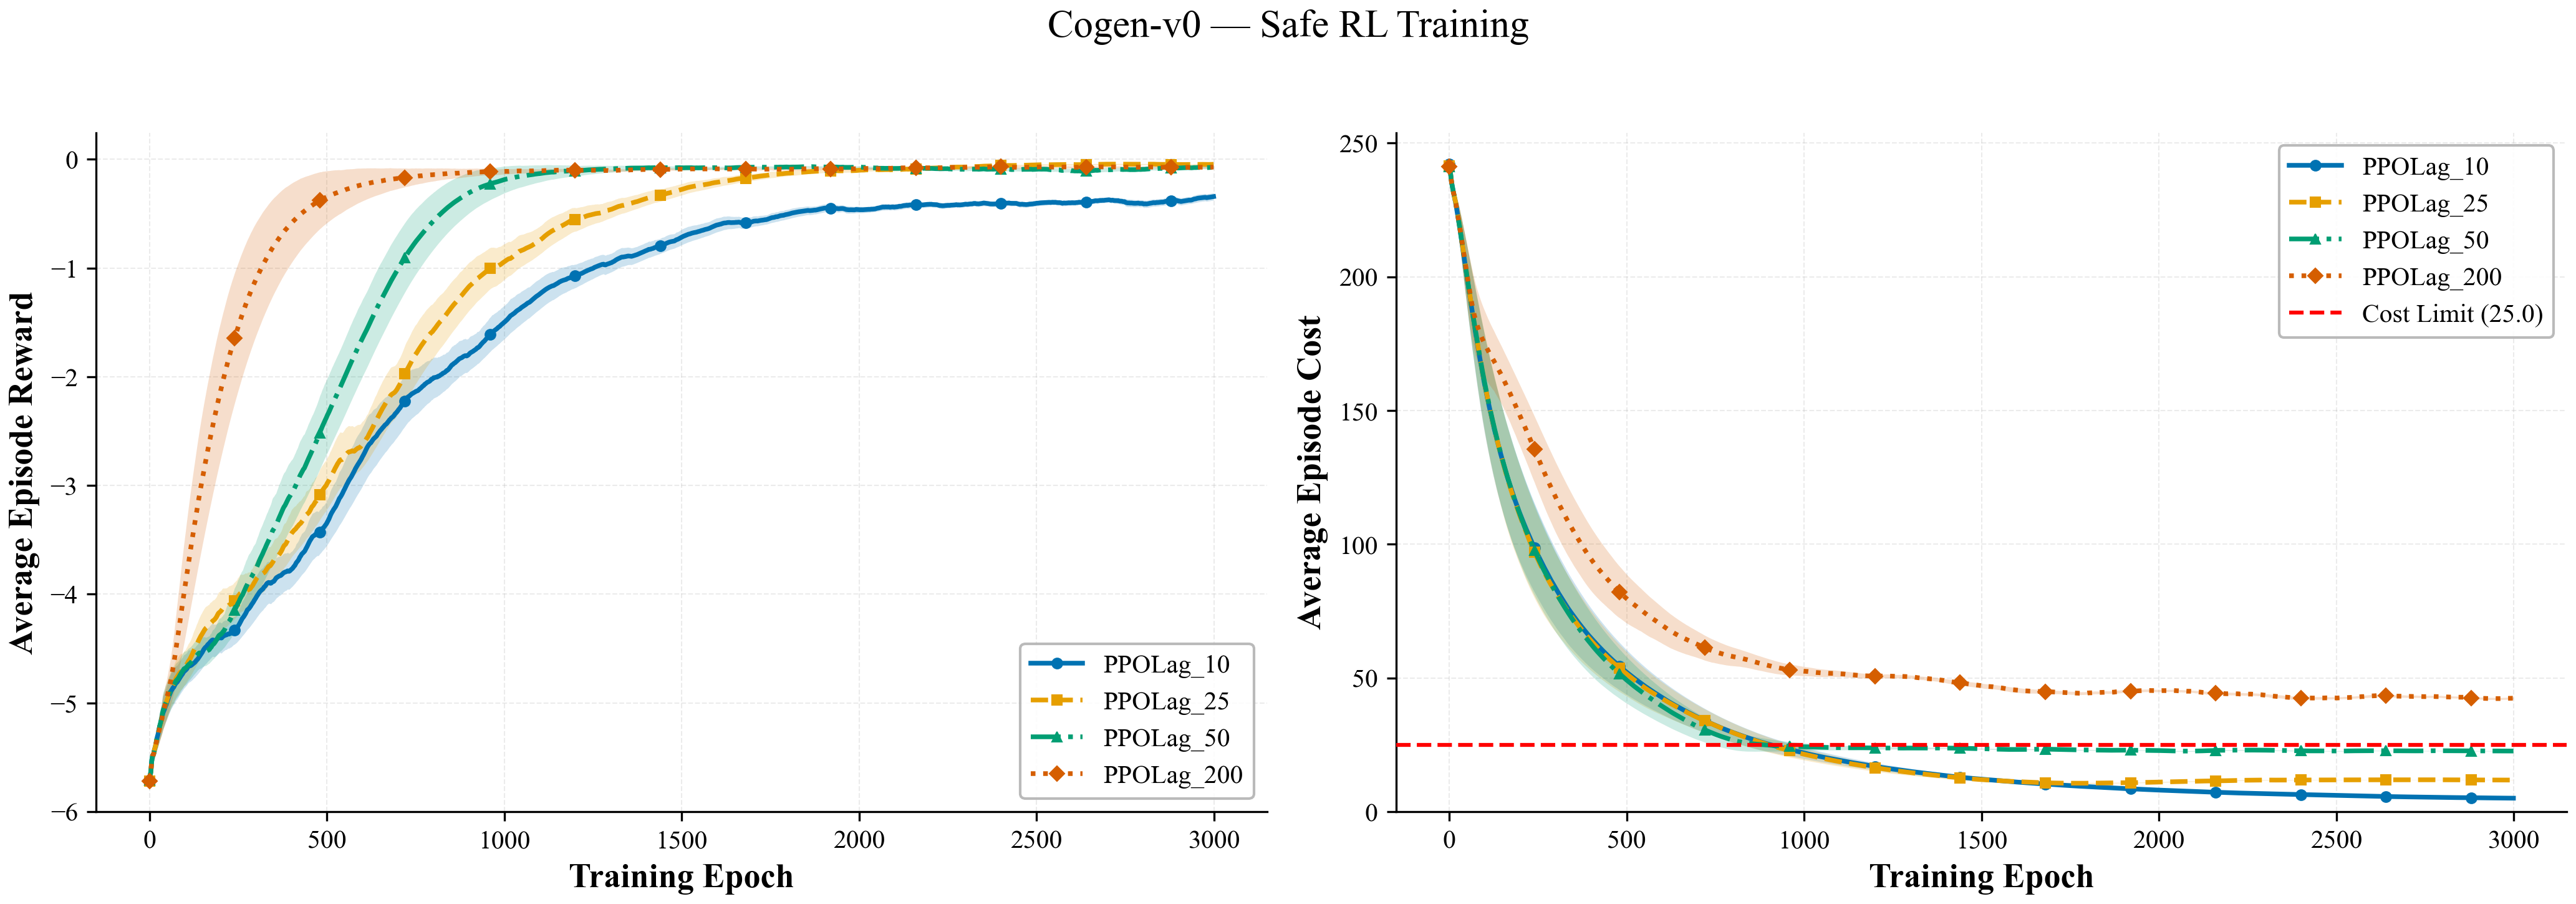
\includegraphics[width=0.9\textwidth]{figures/C_SRL/cogen/saferl_cogen_PPOLag_3000ep_200ema.png}
\caption{Cogen PPOLag: Dual-panel training curves (reward left, cost right) for cost limits $d \in \{10, 25, 50, 200\}$. Clear monotonic differentiation with dashed red line indicating $d = 25$ reference.}
\label{fig:cogen_ppolag}
\end{figure}

% --- Cogen CPO ---
\subsubsection{Cogeneration --- CPO}

CPO reduces cost rapidly ($\sim$500 epochs) but exhibits weaker limit differentiation than PPOLag (\Cref{fig:srl_co_cpo}). The trust-region update converges quickly but lacks the fine-grained control of Lagrangian relaxation.

\begin{figure}[htbp]
\centering
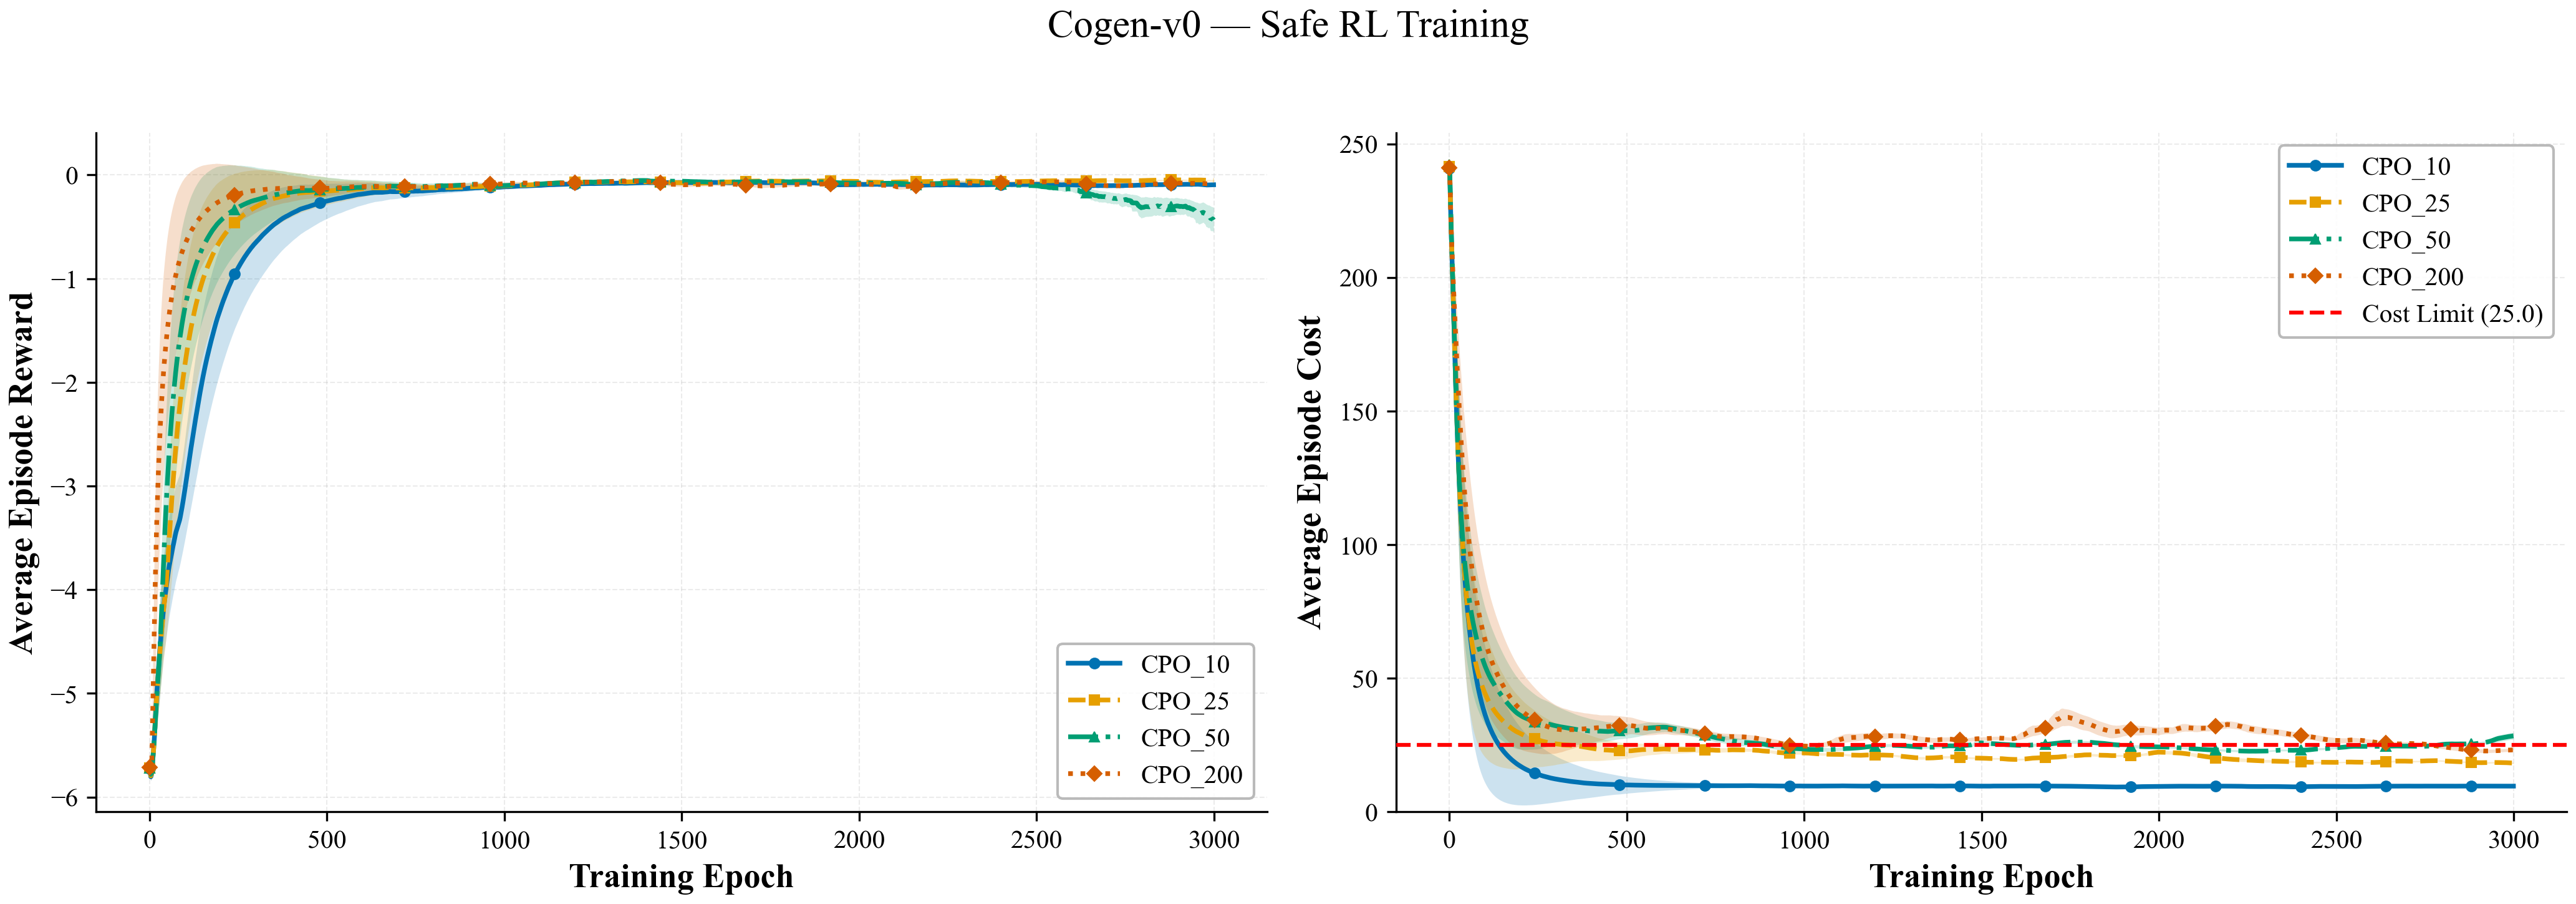
\includegraphics[width=0.9\textwidth]{figures/C_SRL/cogen/saferl_cogen_CPO_3000ep_200ema.png}
\caption{Cogen CPO: Training curves across four cost limits. Trust-region method converges rapidly but shows limited limit differentiation.}
\label{fig:srl_co_cpo}
\end{figure}

% --- Cogen OnCRPO ---
\subsubsection{Cogeneration --- OnCRPO}

OnCRPO shows similar behavior to CPO with rapid cost reduction but produces costs of $12$--$22$ across all four limits with minimal separation (\Cref{fig:srl_co_oncrpo}).

\begin{figure}[htbp]
\centering
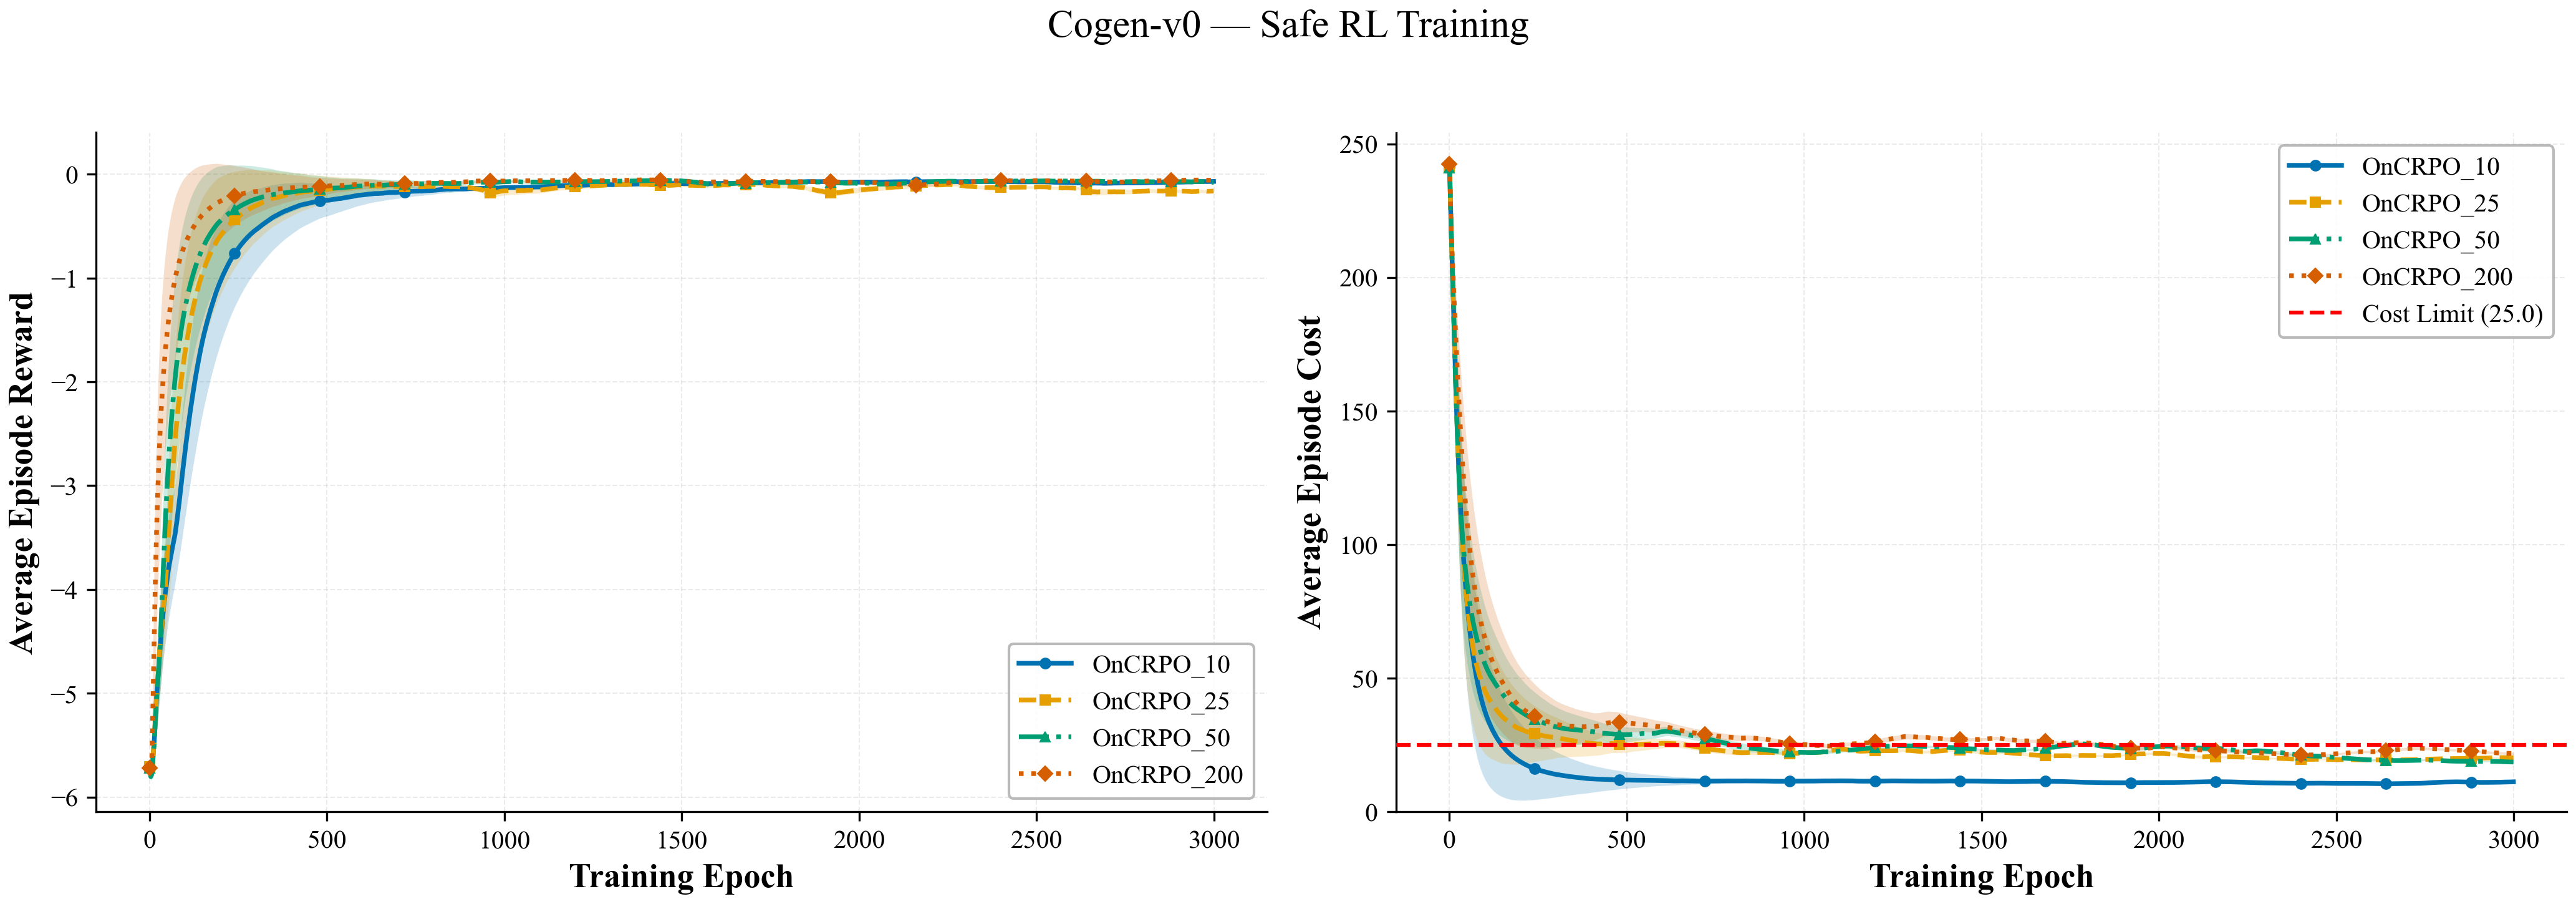
\includegraphics[width=0.9\textwidth]{figures/C_SRL/cogen/saferl_cogen_OnCRPO_3000ep_200ema.png}
\caption{Cogen OnCRPO: Rapid cost reduction but weak limit separation across all four cost limits.}
\label{fig:srl_co_oncrpo}
\end{figure}

% --- Cogen FOCOPS ---
\subsubsection{Cogeneration --- FOCOPS}

FOCOPS shows good monotonic differentiation ($d=10 \to 8$, $d=25 \to 17$, $d=50 \to 28$, $d=200 \to 51$) but converges more slowly than all other algorithms (\Cref{fig:srl_co_focops}).

\begin{figure}[htbp]
\centering
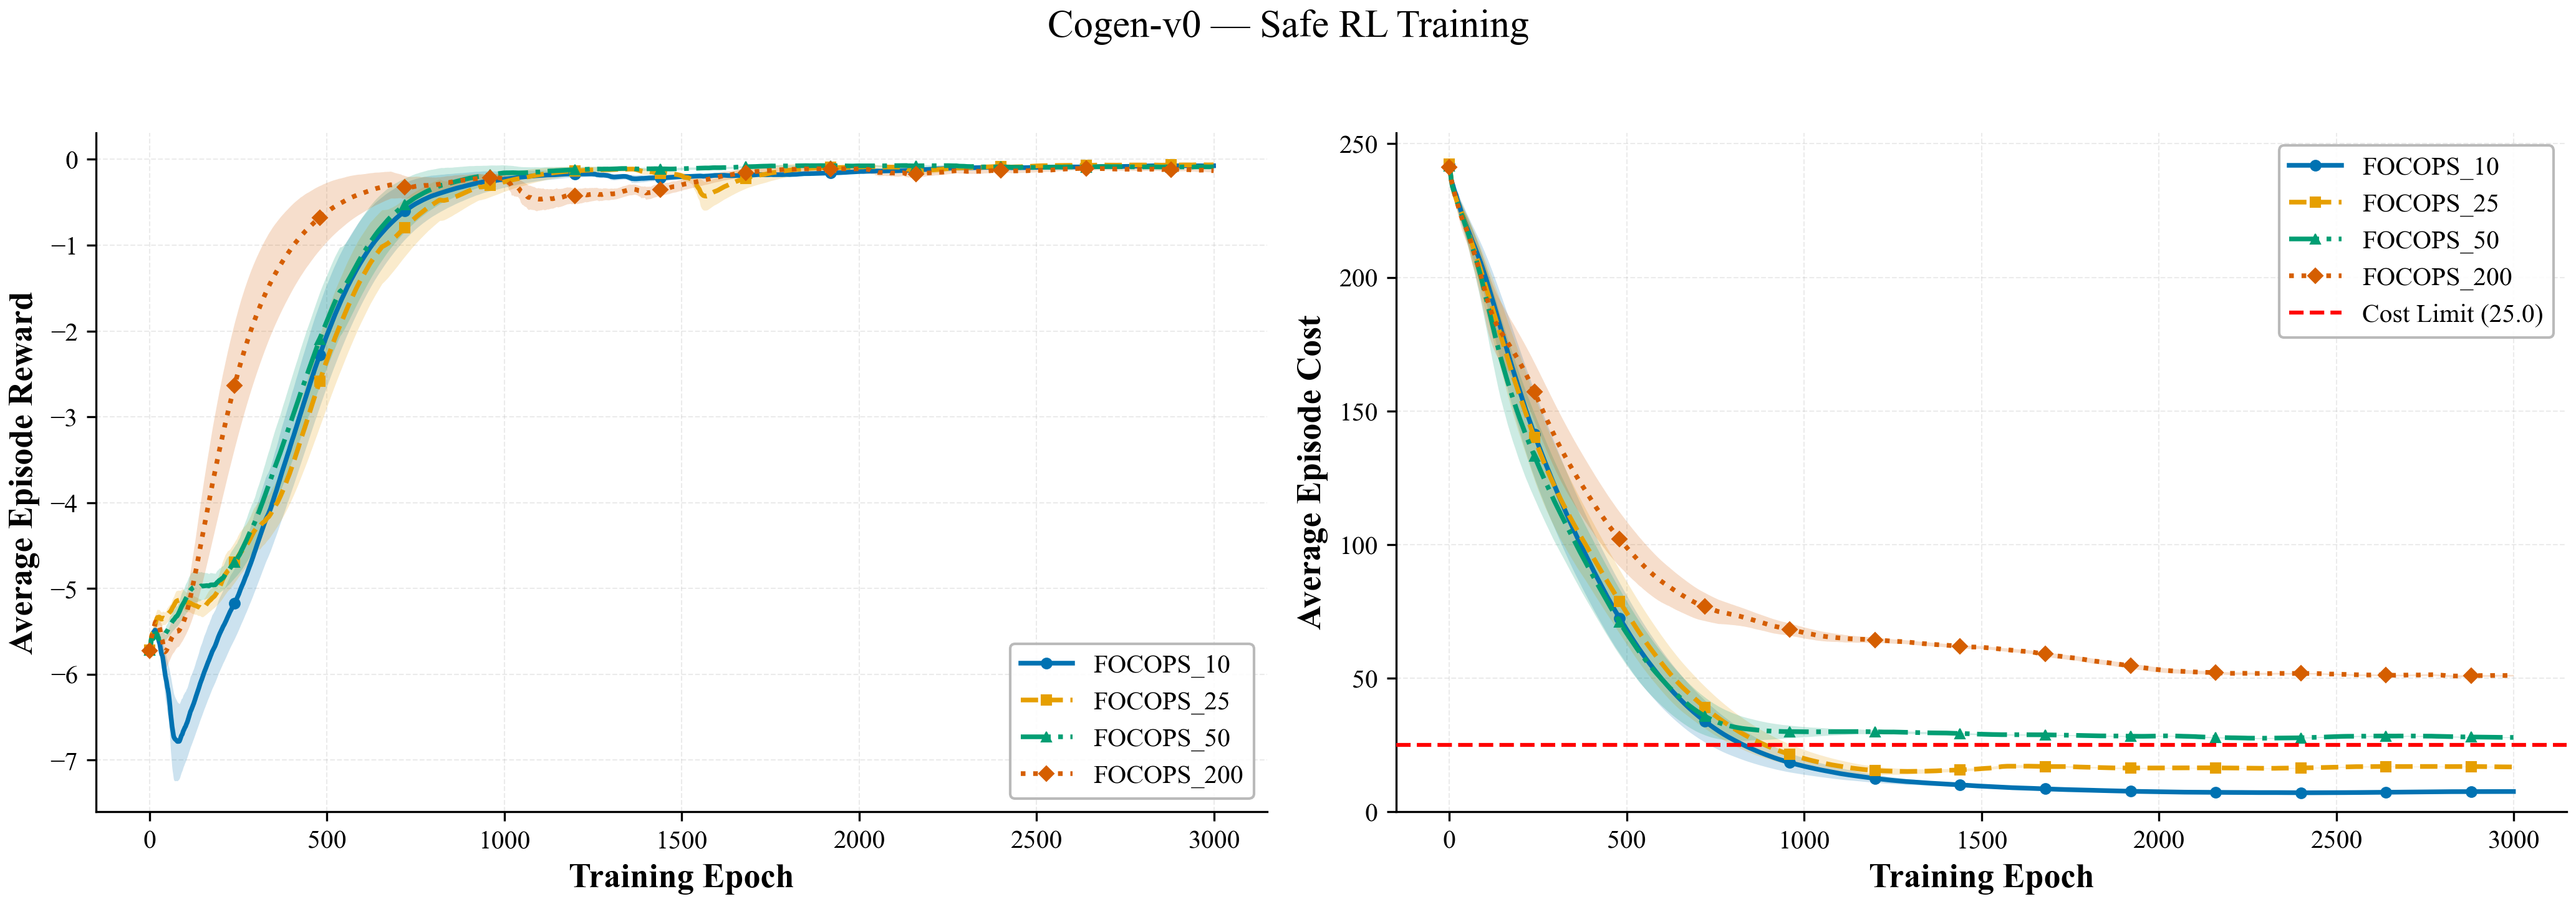
\includegraphics[width=0.9\textwidth]{figures/C_SRL/cogen/saferl_cogen_FOCOPS_3000ep_200ema.png}
\caption{Cogen FOCOPS: Slowest convergence but good monotonic cost differentiation.}
\label{fig:srl_co_focops}
\end{figure}

% --- Cogen Cross-Algorithm ---
\subsubsection{Cogeneration --- Cross-Algorithm Comparisons}

\Cref{fig:srl_co_cmp10,fig:cogen_compare,fig:srl_co_cmp50,fig:srl_co_cmp200} compare all four algorithms at each cost limit. At $d = 25$, the algorithm ranking is:
\begin{equation}
    \text{PPOLag} \succ \text{OnCRPO} \approx \text{CPO} \succ \text{FOCOPS}
\end{equation}

\begin{figure}[htbp]
\centering
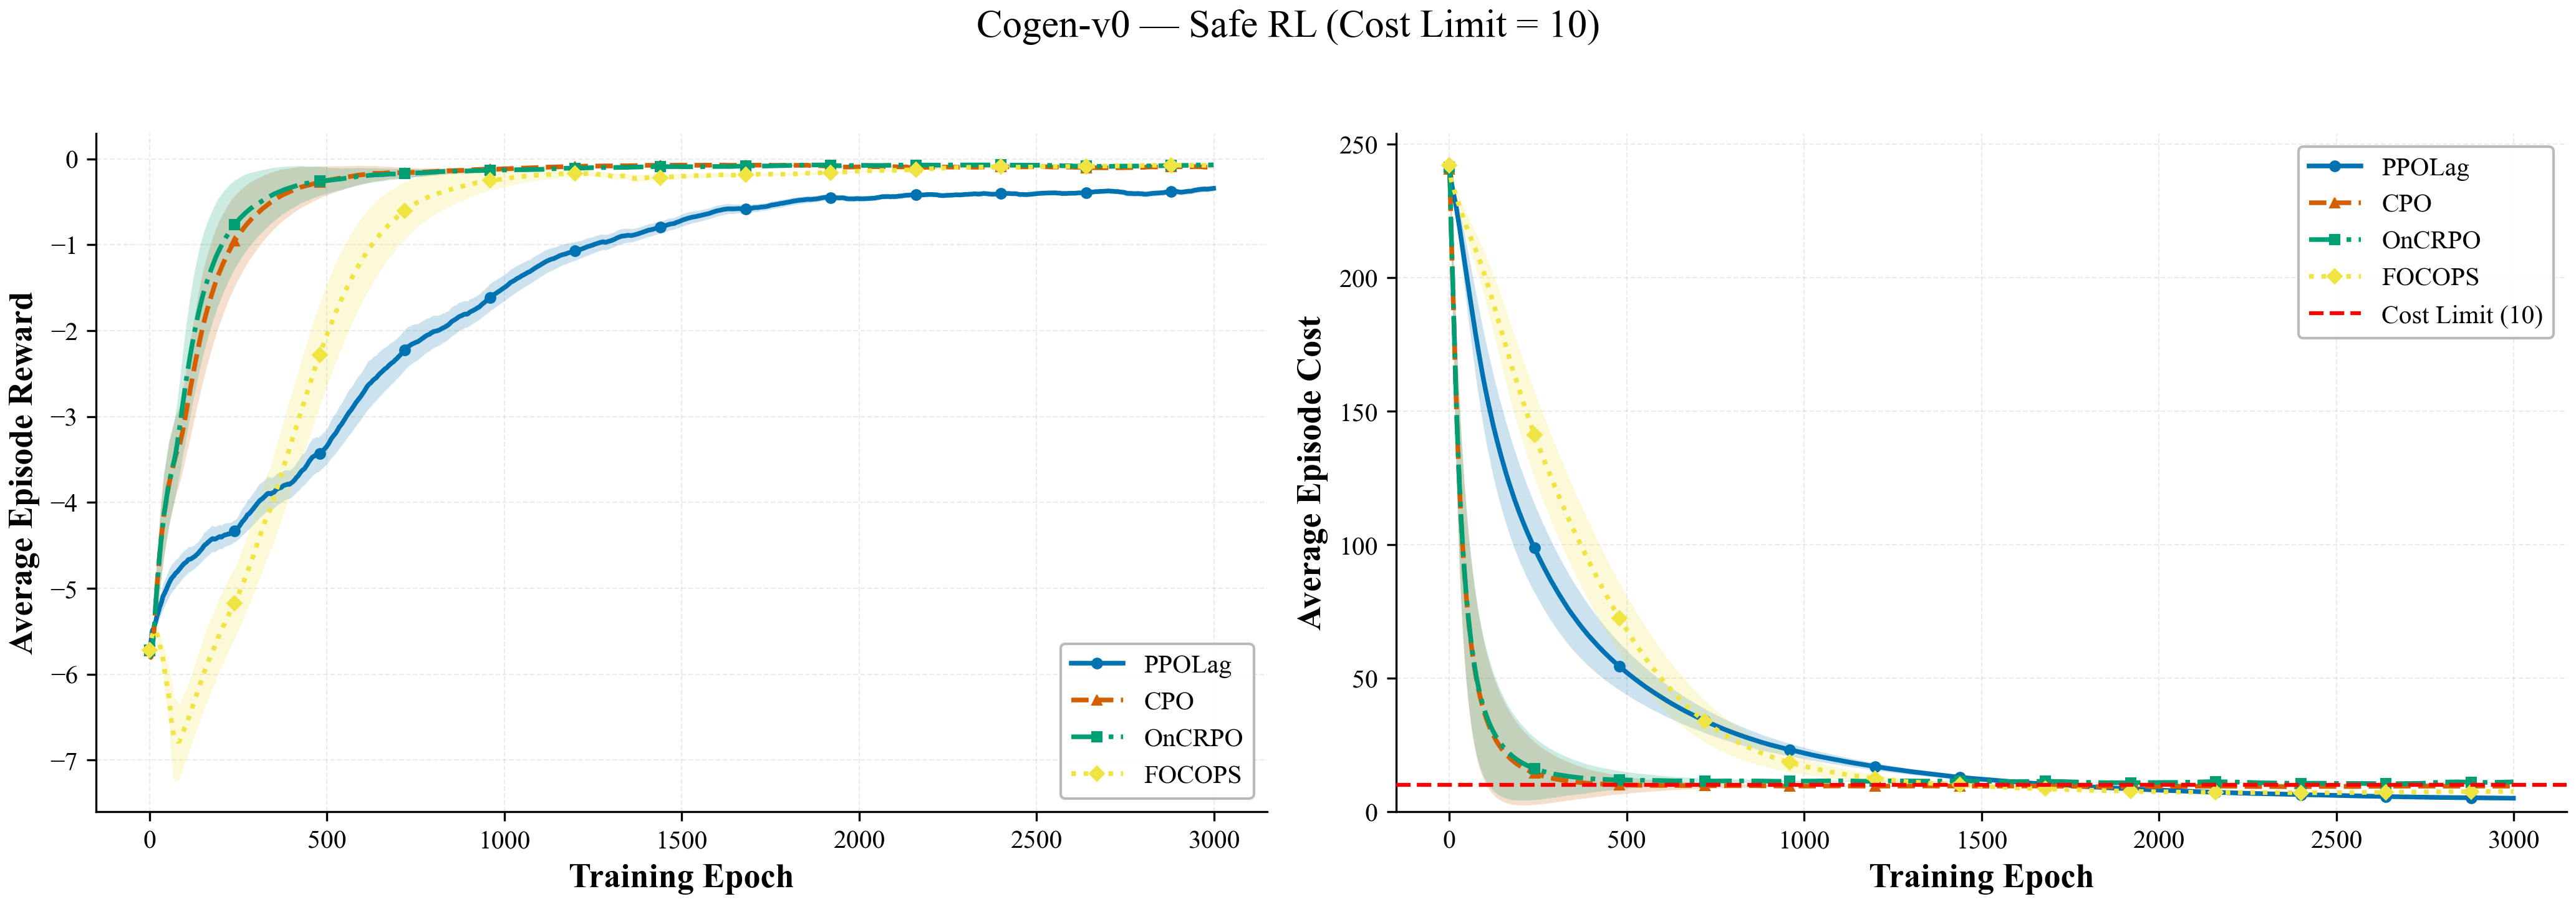
\includegraphics[width=0.9\textwidth]{figures/C_SRL/cogen/saferl_cogen_compare_CL10_3000ep_200ema.png}
\caption{Cogen cross-algorithm comparison at tightest limit $d = 10$.}
\label{fig:srl_co_cmp10}
\end{figure}

\begin{figure}[htbp]
\centering
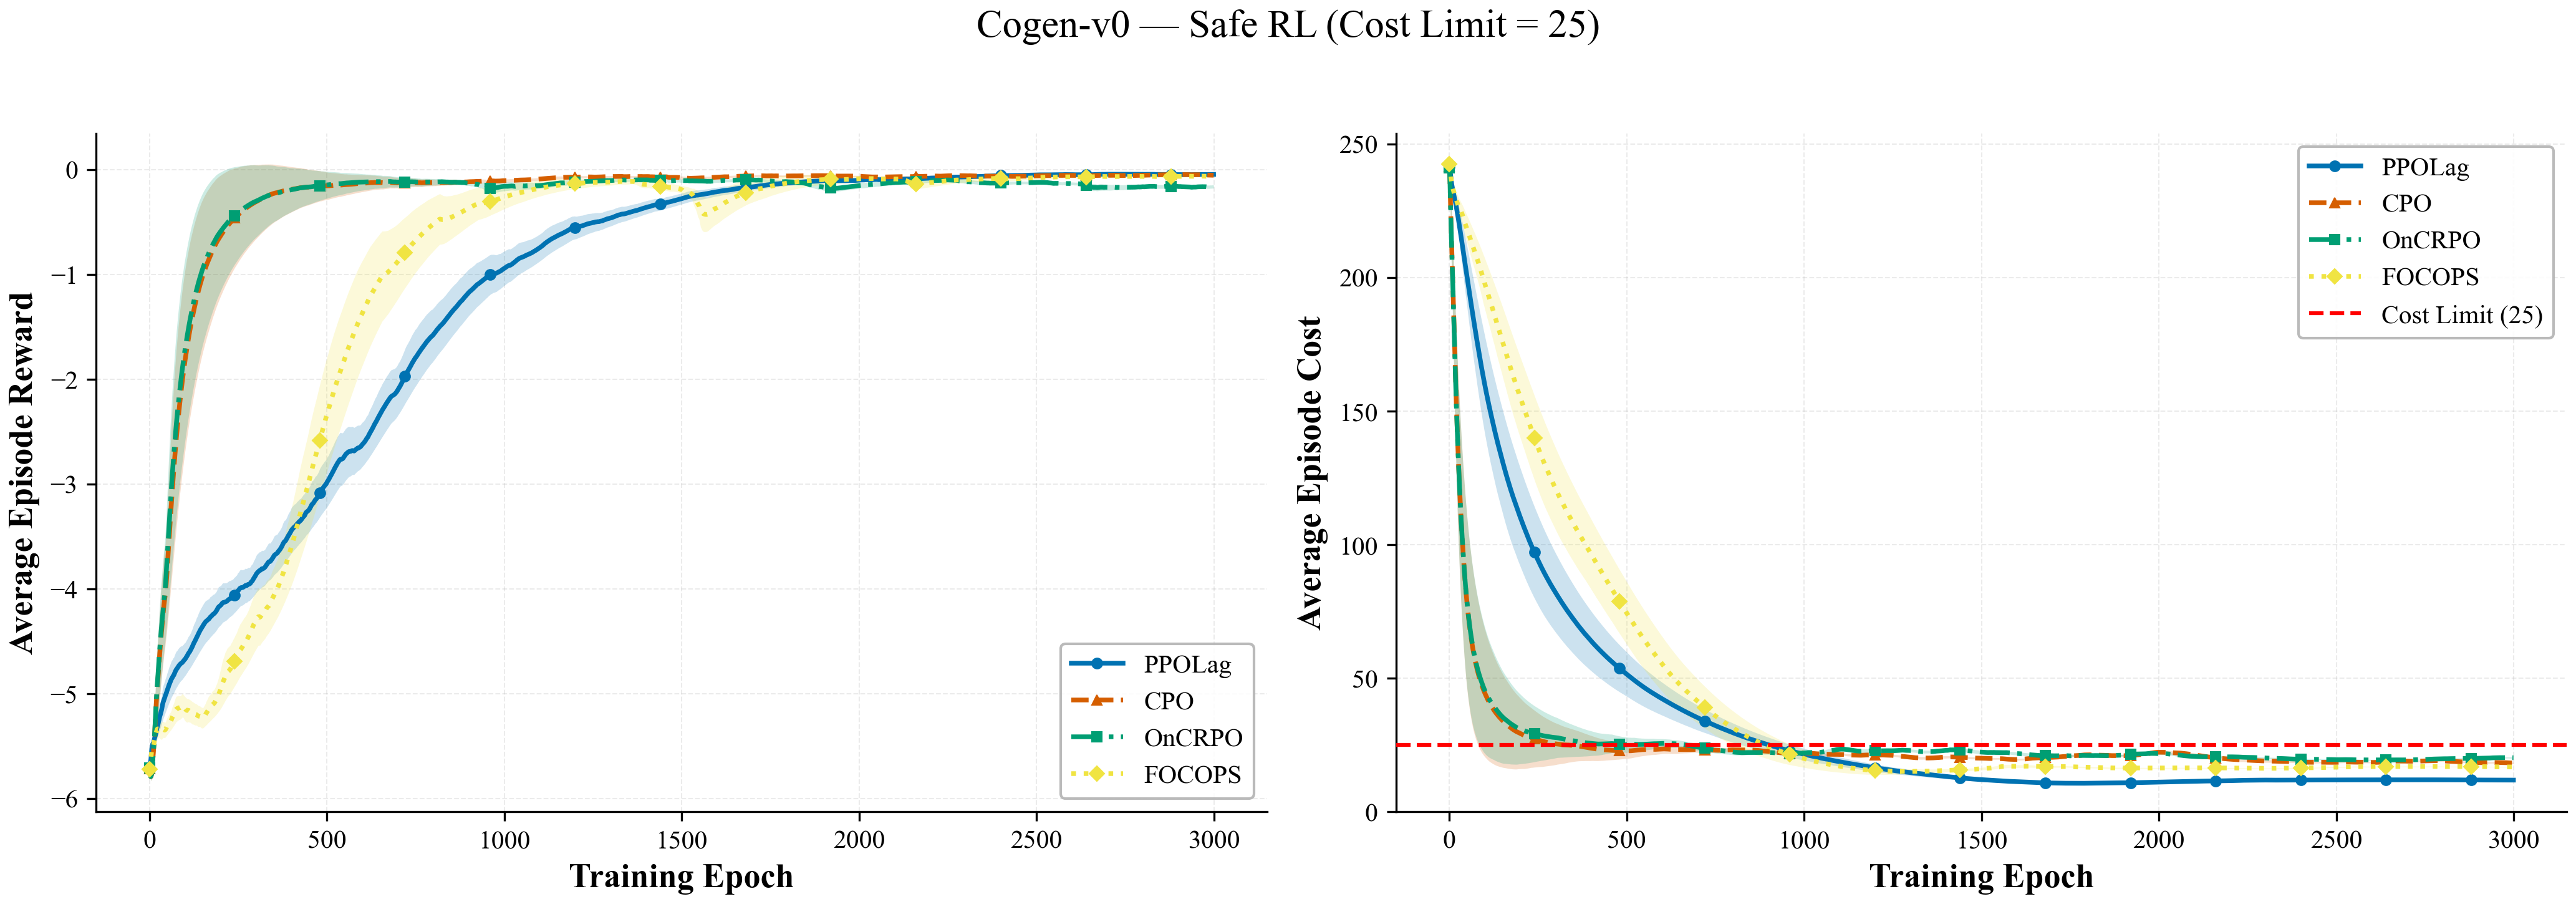
\includegraphics[width=0.9\textwidth]{figures/C_SRL/cogen/saferl_cogen_compare_CL25_3000ep_200ema.png}
\caption{Cogen cross-algorithm comparison at $d = 25$. PPOLag achieves the best reward while satisfying the constraint; FOCOPS converges slowest.}
\label{fig:cogen_compare}
\end{figure}

\begin{figure}[htbp]
\centering
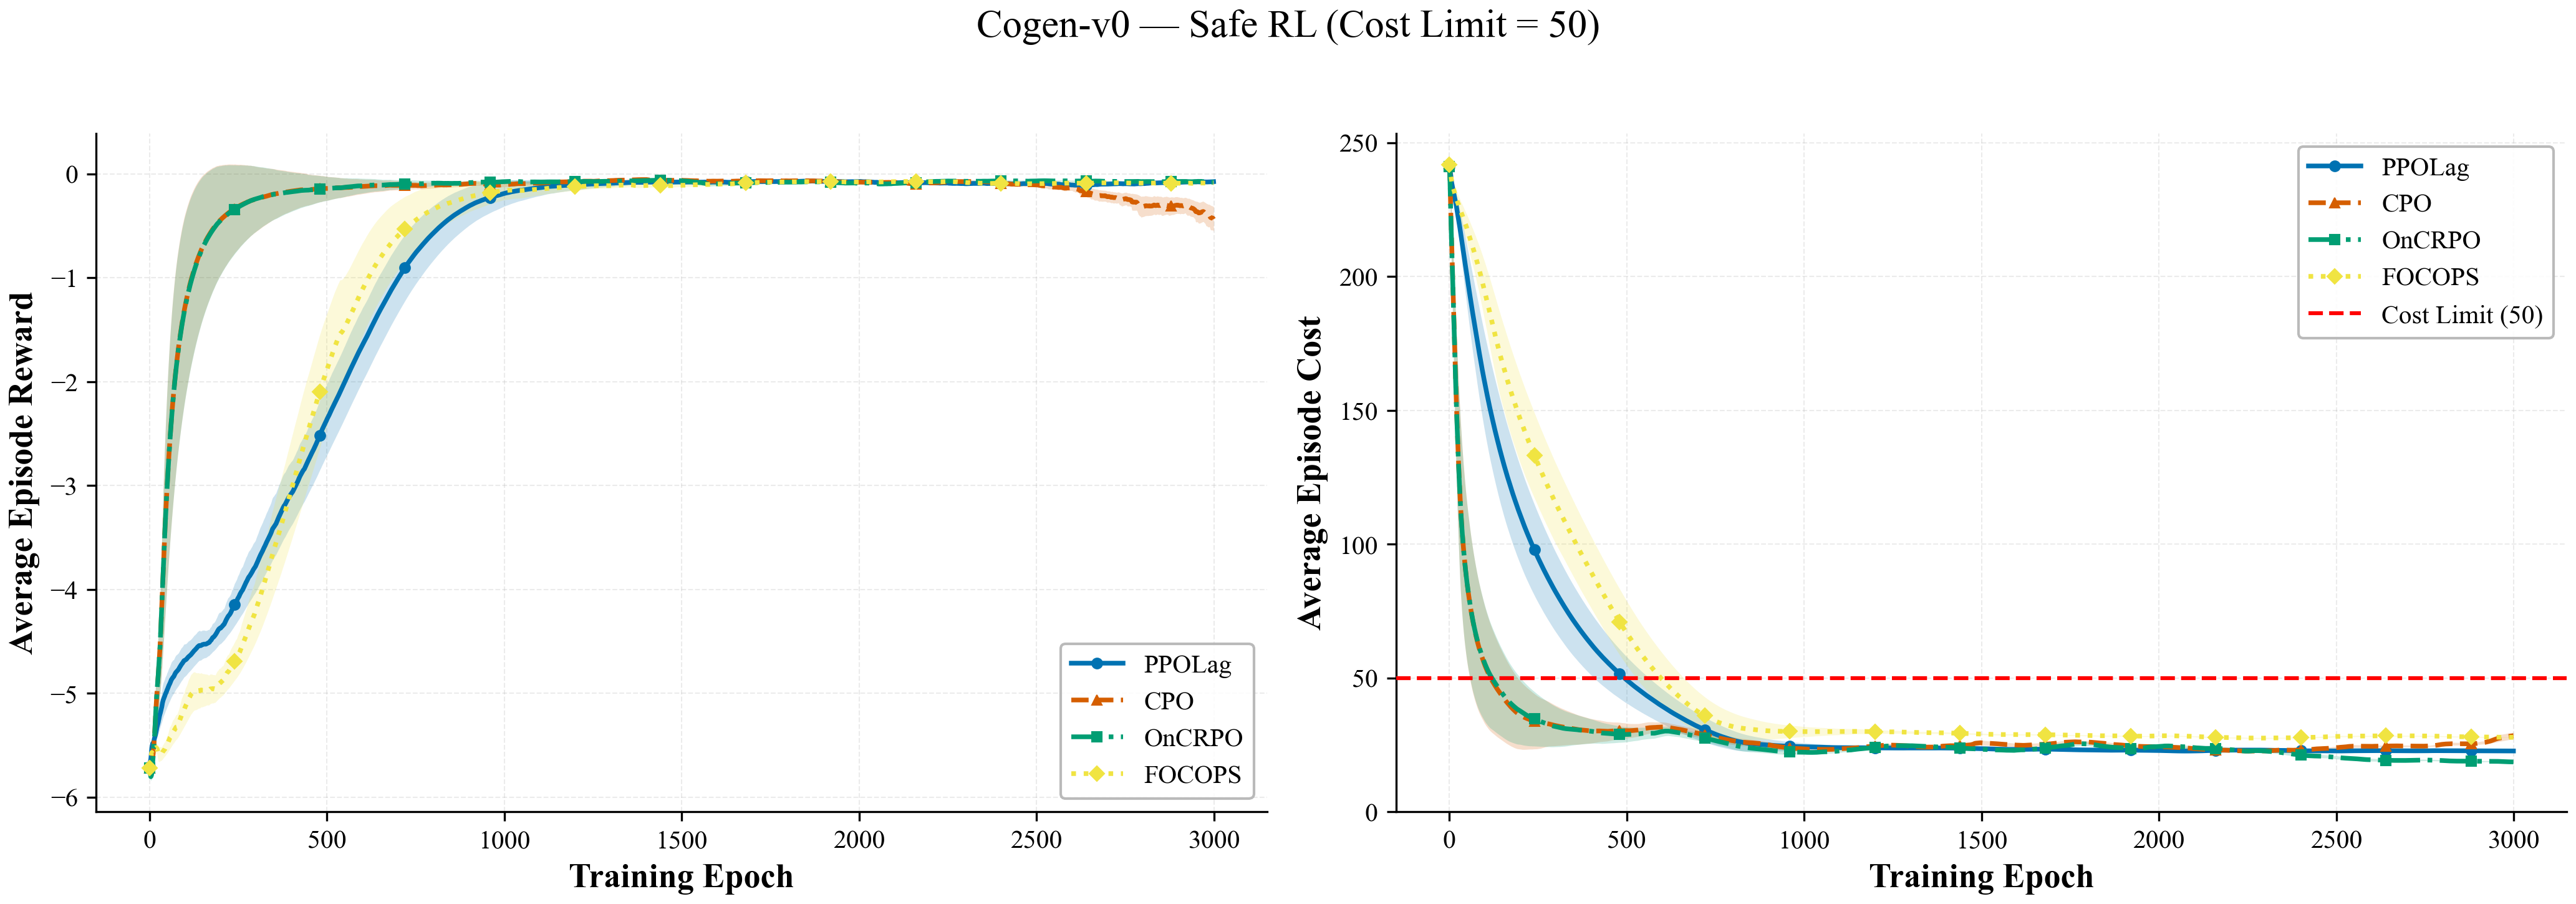
\includegraphics[width=0.9\textwidth]{figures/C_SRL/cogen/saferl_cogen_compare_CL50_3000ep_200ema.png}
\caption{Cogen cross-algorithm comparison at moderate limit $d = 50$.}
\label{fig:srl_co_cmp50}
\end{figure}

\begin{figure}[htbp]
\centering
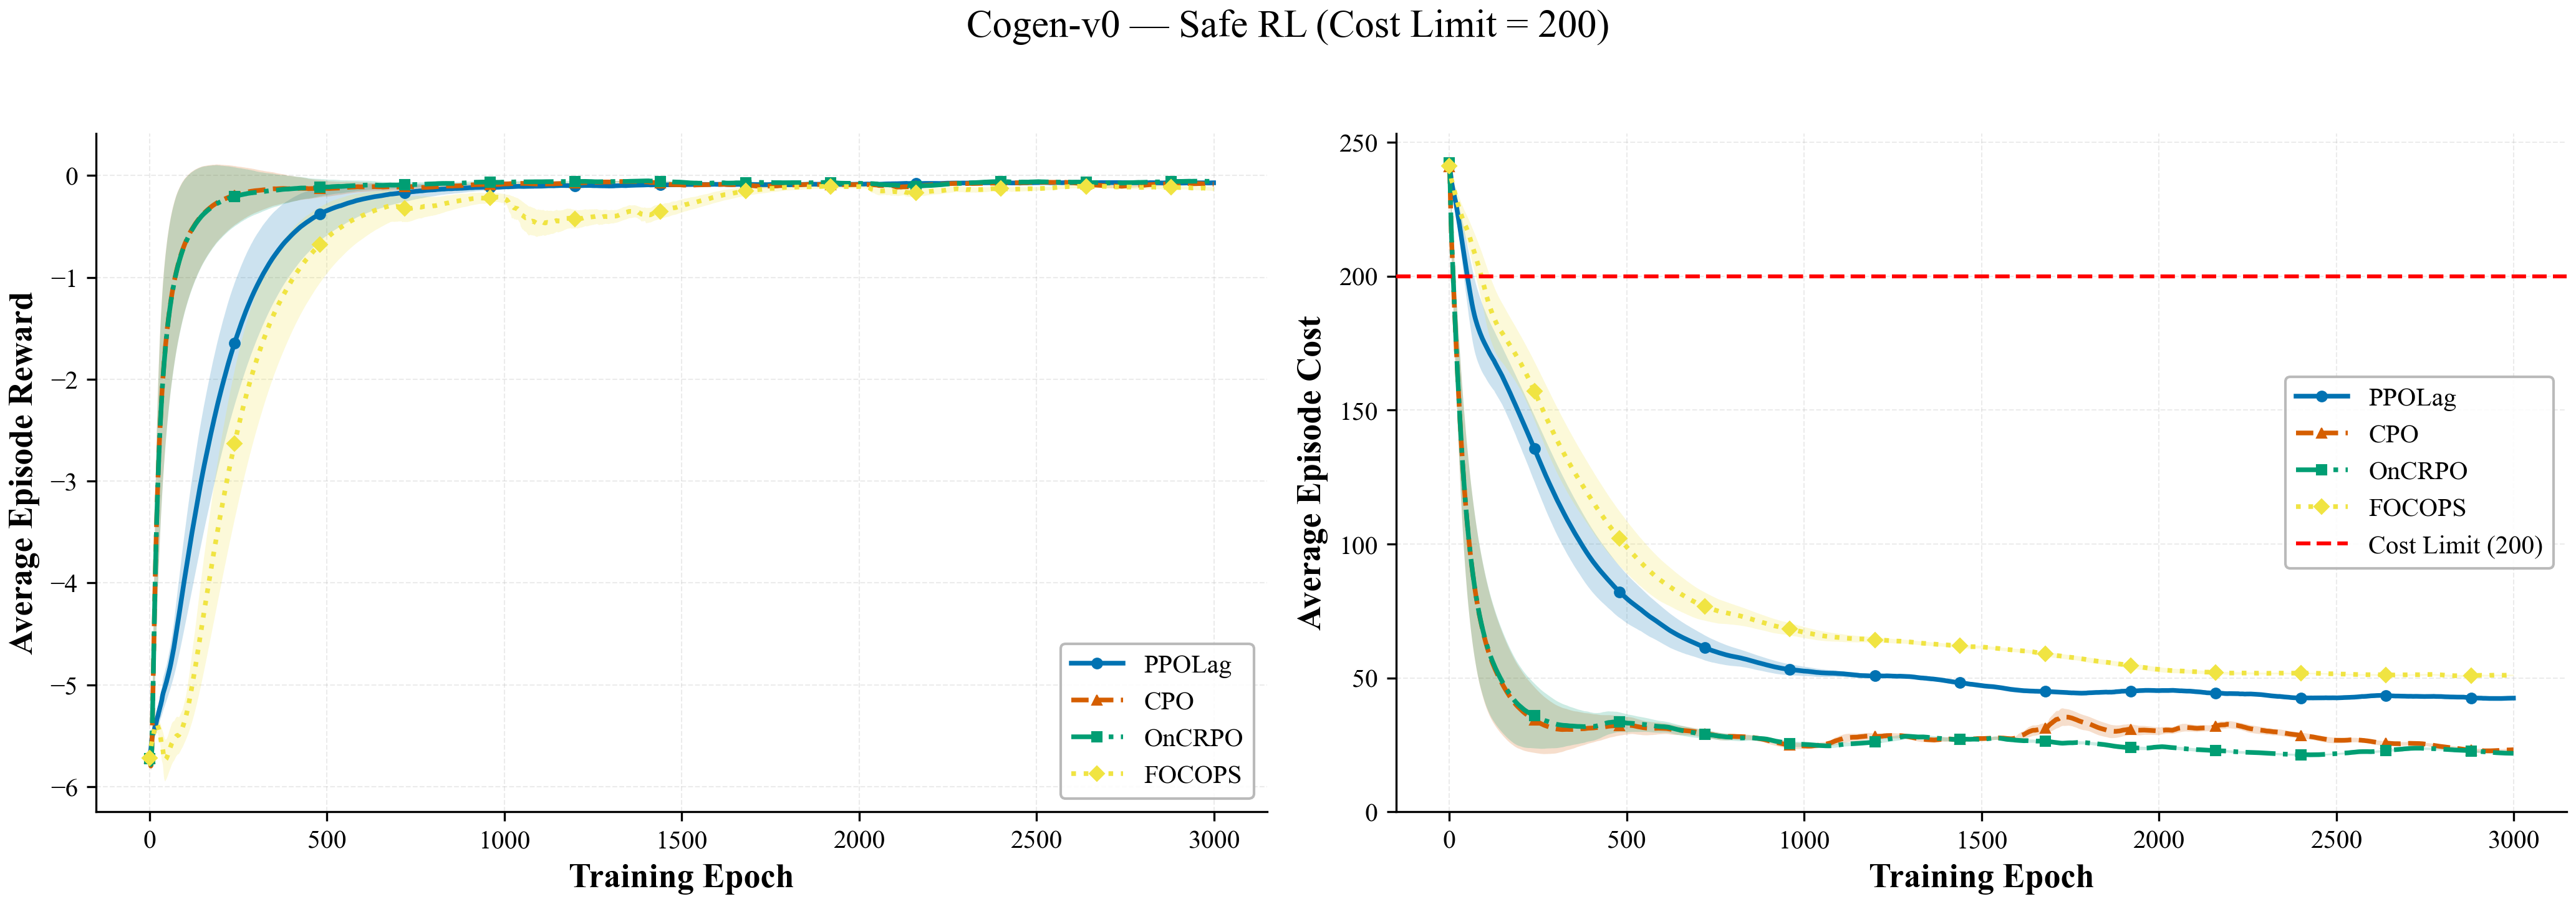
\includegraphics[width=0.9\textwidth]{figures/C_SRL/cogen/saferl_cogen_compare_CL200_3000ep_200ema.png}
\caption{Cogen cross-algorithm comparison at loosest limit $d = 200$.}
\label{fig:srl_co_cmp200}
\end{figure}

% ------------------------------------------------------------
\subsection{EV Charging: Precise Constraint Tracking}
\label{sec:saferl_ev}

The EV Charging CMDP cost (excess charge violations, $\alpha_c = 100$) is structurally orthogonal to the reward. With cost limits $d \in \{3, 5, 25\}$, all algorithms demonstrate strong constraint satisfaction (\Cref{tab:ev_saferl}).

\begin{table}[htbp]
\centering
\caption{EV Charging Safe RL: Final episode cost by algorithm and limit. \textbf{Bold}: satisfies $C \leq d$.}
\label{tab:ev_saferl}
\begin{tabular}{@{}lcccc@{}}
\toprule
\textbf{$d$} & \textbf{PPOLag} & \textbf{CPO} & \textbf{OnCRPO} & \textbf{FOCOPS} \\
\midrule
$3$  & $\mathbf{2.6}$ & $3.3$ & $4.5$ & $\mathbf{3.1}$ \\
$5$  & $\mathbf{5.1}$ & $\mathbf{5.7}$ & $6.9$ & $\mathbf{3.6}$ \\
$25$ & $\mathbf{21.5}$ & $\mathbf{20.7}$ & $27.5$ & $26.2$ \\
\bottomrule
\end{tabular}
\end{table}

% --- EV PPOLag ---
\subsubsection{EV Charging --- PPOLag}

PPOLag achieves near-exact constraint satisfaction at all levels (\Cref{fig:ev_ppolag}), demonstrating that Lagrangian relaxation provides precise control over network constraint violations. Tight limits ($d = 3, 5$) are precisely satisfied; loose limits ($d = 1000, 10000$) show natural cost reduction without active constraint enforcement.

\begin{figure}[htbp]
\centering
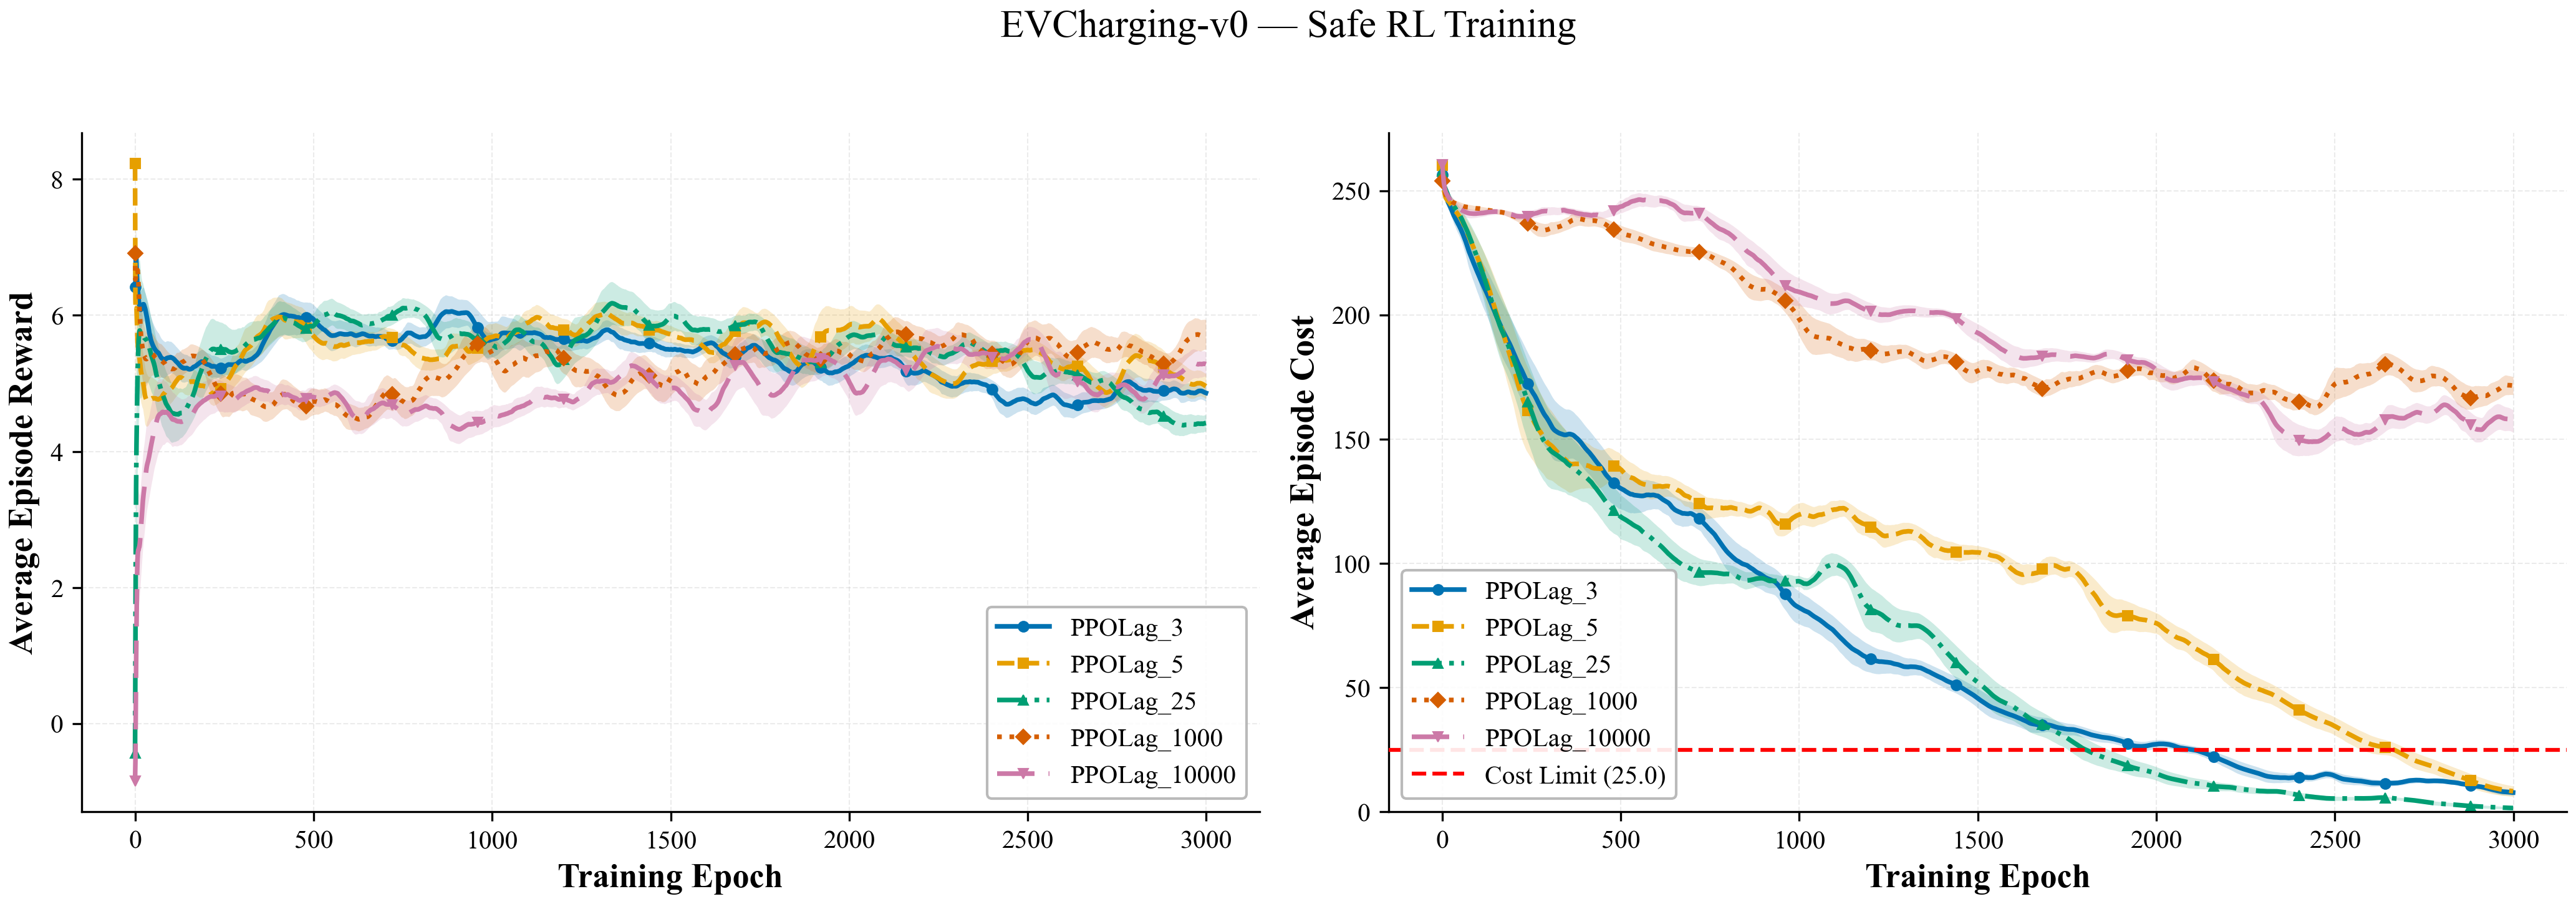
\includegraphics[width=0.9\textwidth]{figures/C_SRL/evcharging/saferl_evcharging_PPOLag_3000ep_200ema.png}
\caption{EV Charging PPOLag: Training curves across five cost limits. Tight limits ($d = 3, 5$) are precisely satisfied; loose limits show natural cost reduction.}
\label{fig:ev_ppolag}
\end{figure}

% --- EV CPO ---
\subsubsection{EV Charging --- CPO}

CPO satisfies the constraint at moderate and loose limits but slightly overshoots at the tightest limit ($d = 3$, final cost $= 3.3$), as shown in \Cref{fig:srl_ev_cpo}.

\begin{figure}[htbp]
\centering
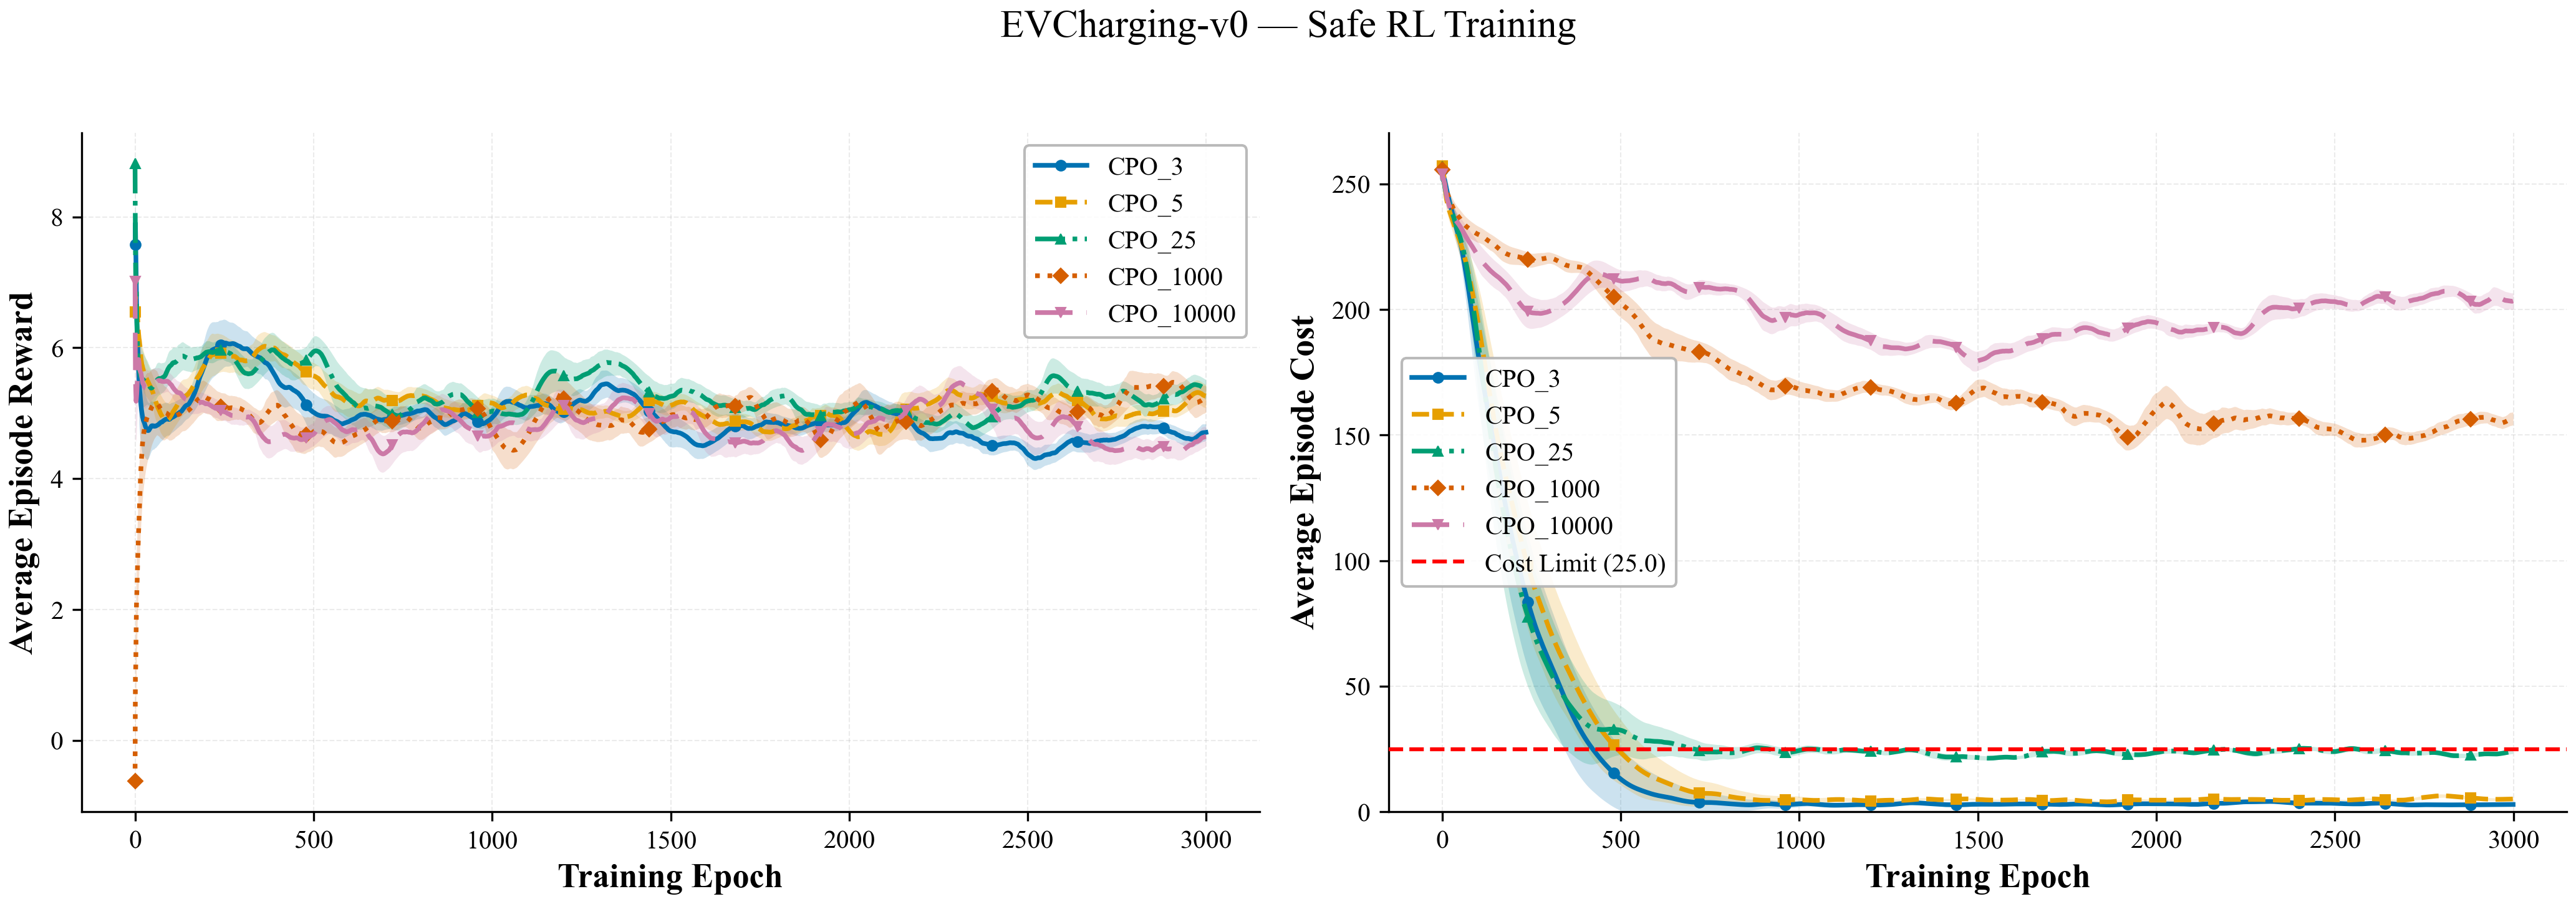
\includegraphics[width=0.9\textwidth]{figures/C_SRL/evcharging/saferl_evcharging_CPO_3000ep_200ema.png}
\caption{EV Charging CPO: Training curves across cost limits.}
\label{fig:srl_ev_cpo}
\end{figure}

% --- EV OnCRPO ---
\subsubsection{EV Charging --- OnCRPO}

OnCRPO consistently overshoots the prescribed cost limits (\Cref{fig:srl_ev_oncrpo}), with final costs exceeding the target at all three levels ($d = 3 \to 4.5$, $d = 5 \to 6.9$, $d = 25 \to 27.5$).

\begin{figure}[htbp]
\centering
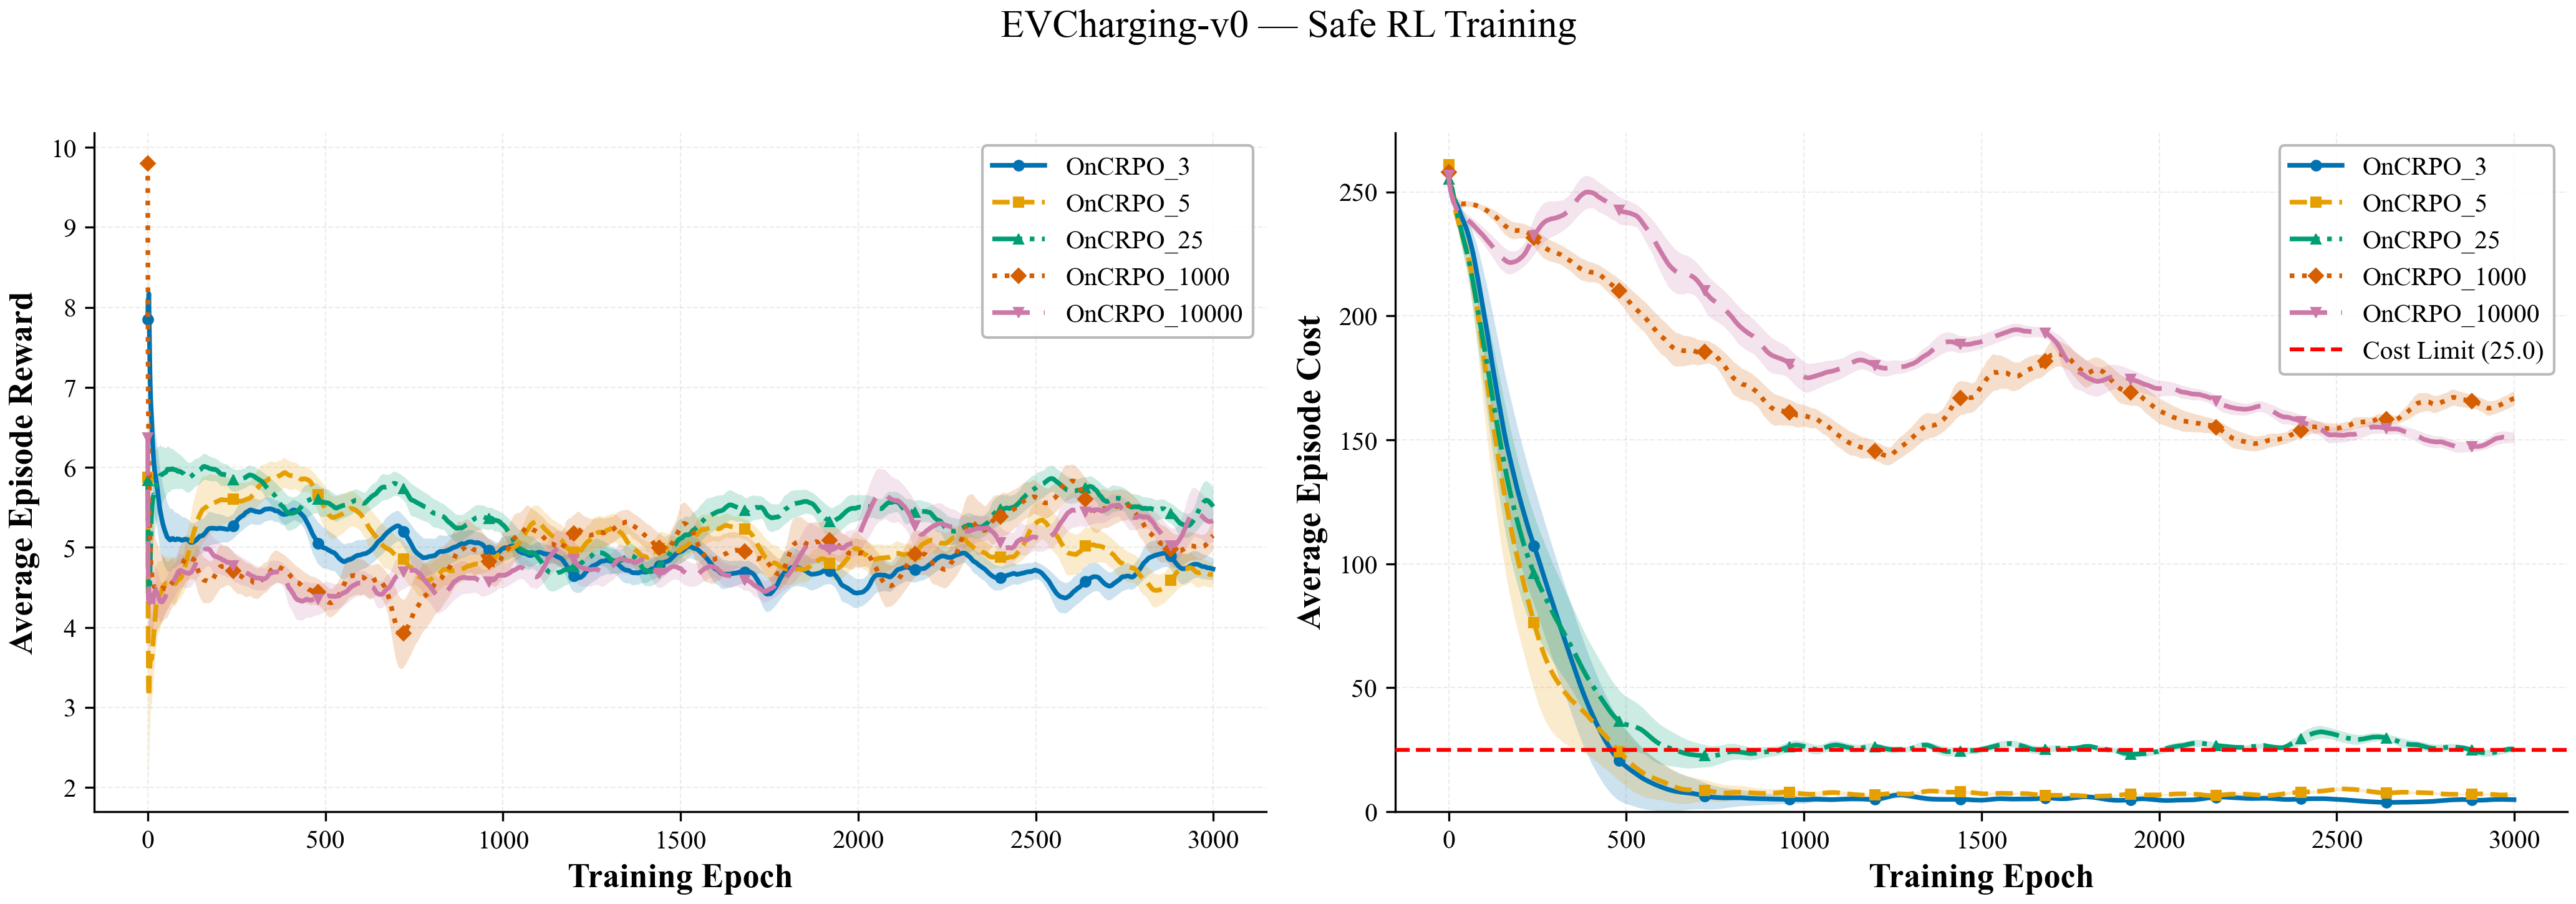
\includegraphics[width=0.9\textwidth]{figures/C_SRL/evcharging/saferl_evcharging_OnCRPO_3000ep_200ema.png}
\caption{EV Charging OnCRPO: Training curves across cost limits.}
\label{fig:srl_ev_oncrpo}
\end{figure}

% --- EV FOCOPS ---
\subsubsection{EV Charging --- FOCOPS}

FOCOPS achieves strong constraint satisfaction at tight limits ($d = 3 \to 3.1$, $d = 5 \to 3.6$) but slightly overshoots at loose limits ($d = 25 \to 26.2$), as shown in \Cref{fig:srl_ev_focops}.

\begin{figure}[htbp]
\centering
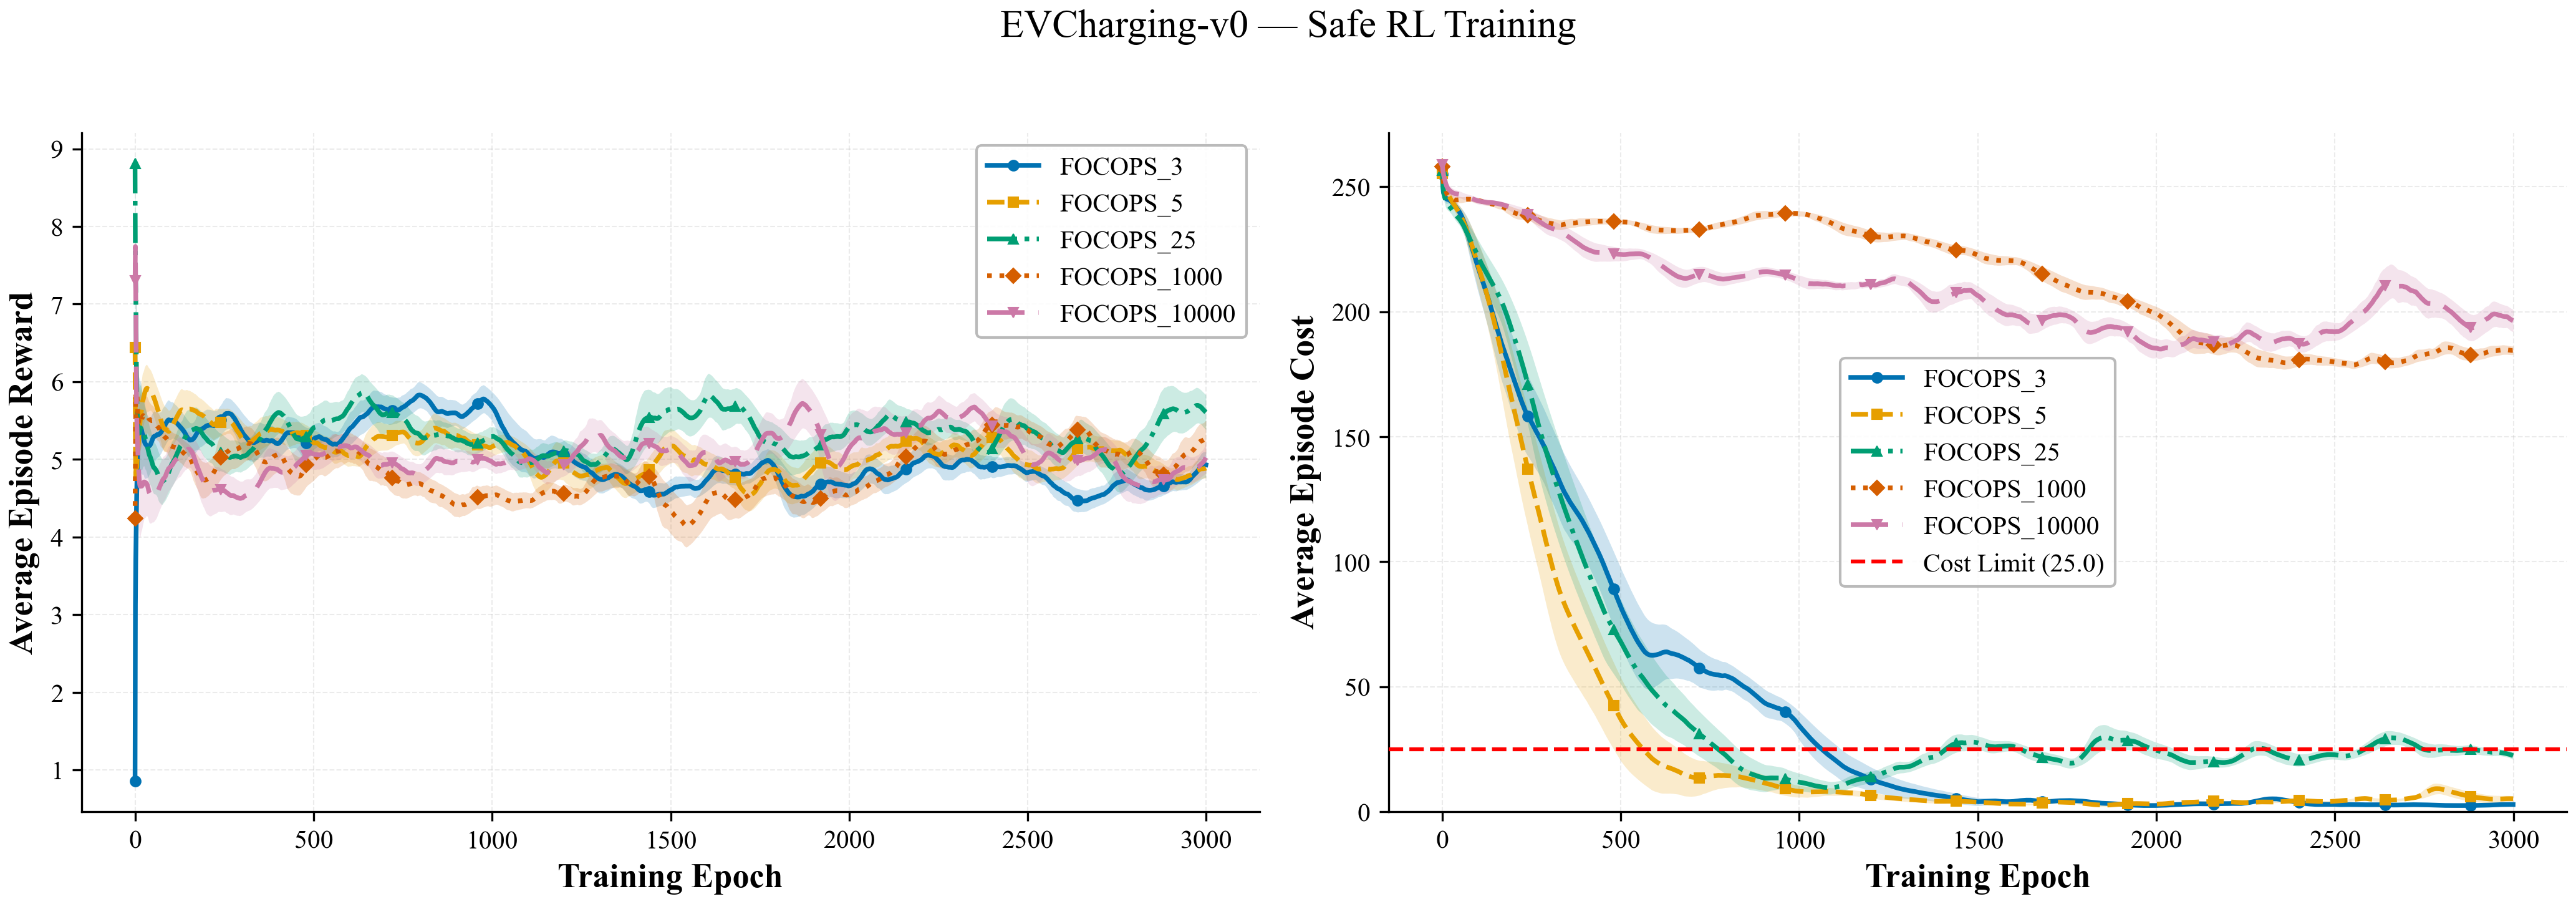
\includegraphics[width=0.9\textwidth]{figures/C_SRL/evcharging/saferl_evcharging_FOCOPS_3000ep_200ema.png}
\caption{EV Charging FOCOPS: Training curves across cost limits.}
\label{fig:srl_ev_focops}
\end{figure}

% --- EV Cross-Algorithm ---
\subsubsection{EV Charging --- Cross-Algorithm Comparisons}

\Cref{fig:srl_ev_cmp3,fig:srl_ev_cmp25} compare all four algorithms at the tightest and moderate cost limits respectively.

\begin{figure}[htbp]
\centering
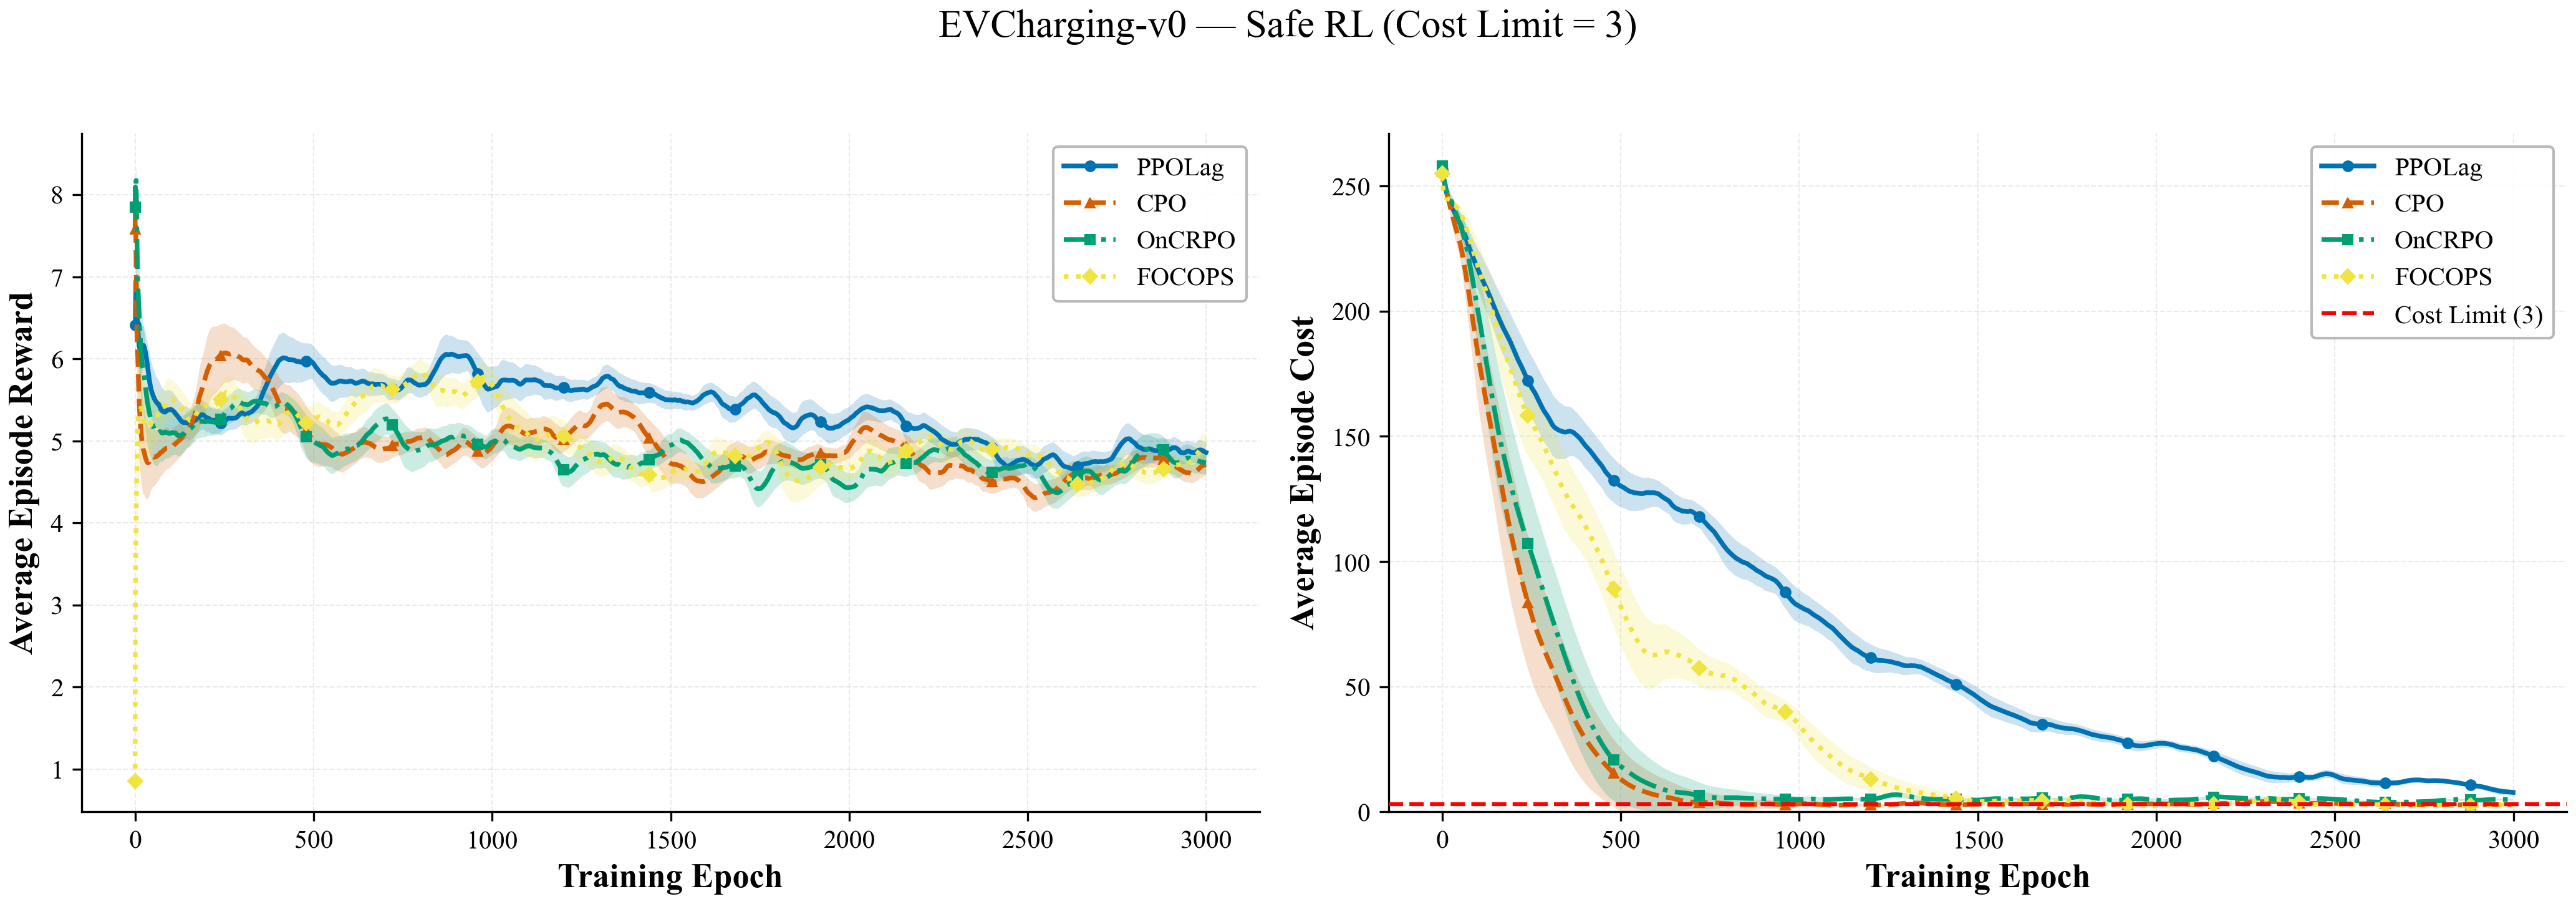
\includegraphics[width=0.9\textwidth]{figures/C_SRL/evcharging/saferl_evcharging_compare_CL3_3000ep_200ema.png}
\caption{EV Charging cross-algorithm comparison at tightest limit $d = 3$.}
\label{fig:srl_ev_cmp3}
\end{figure}

\begin{figure}[htbp]
\centering
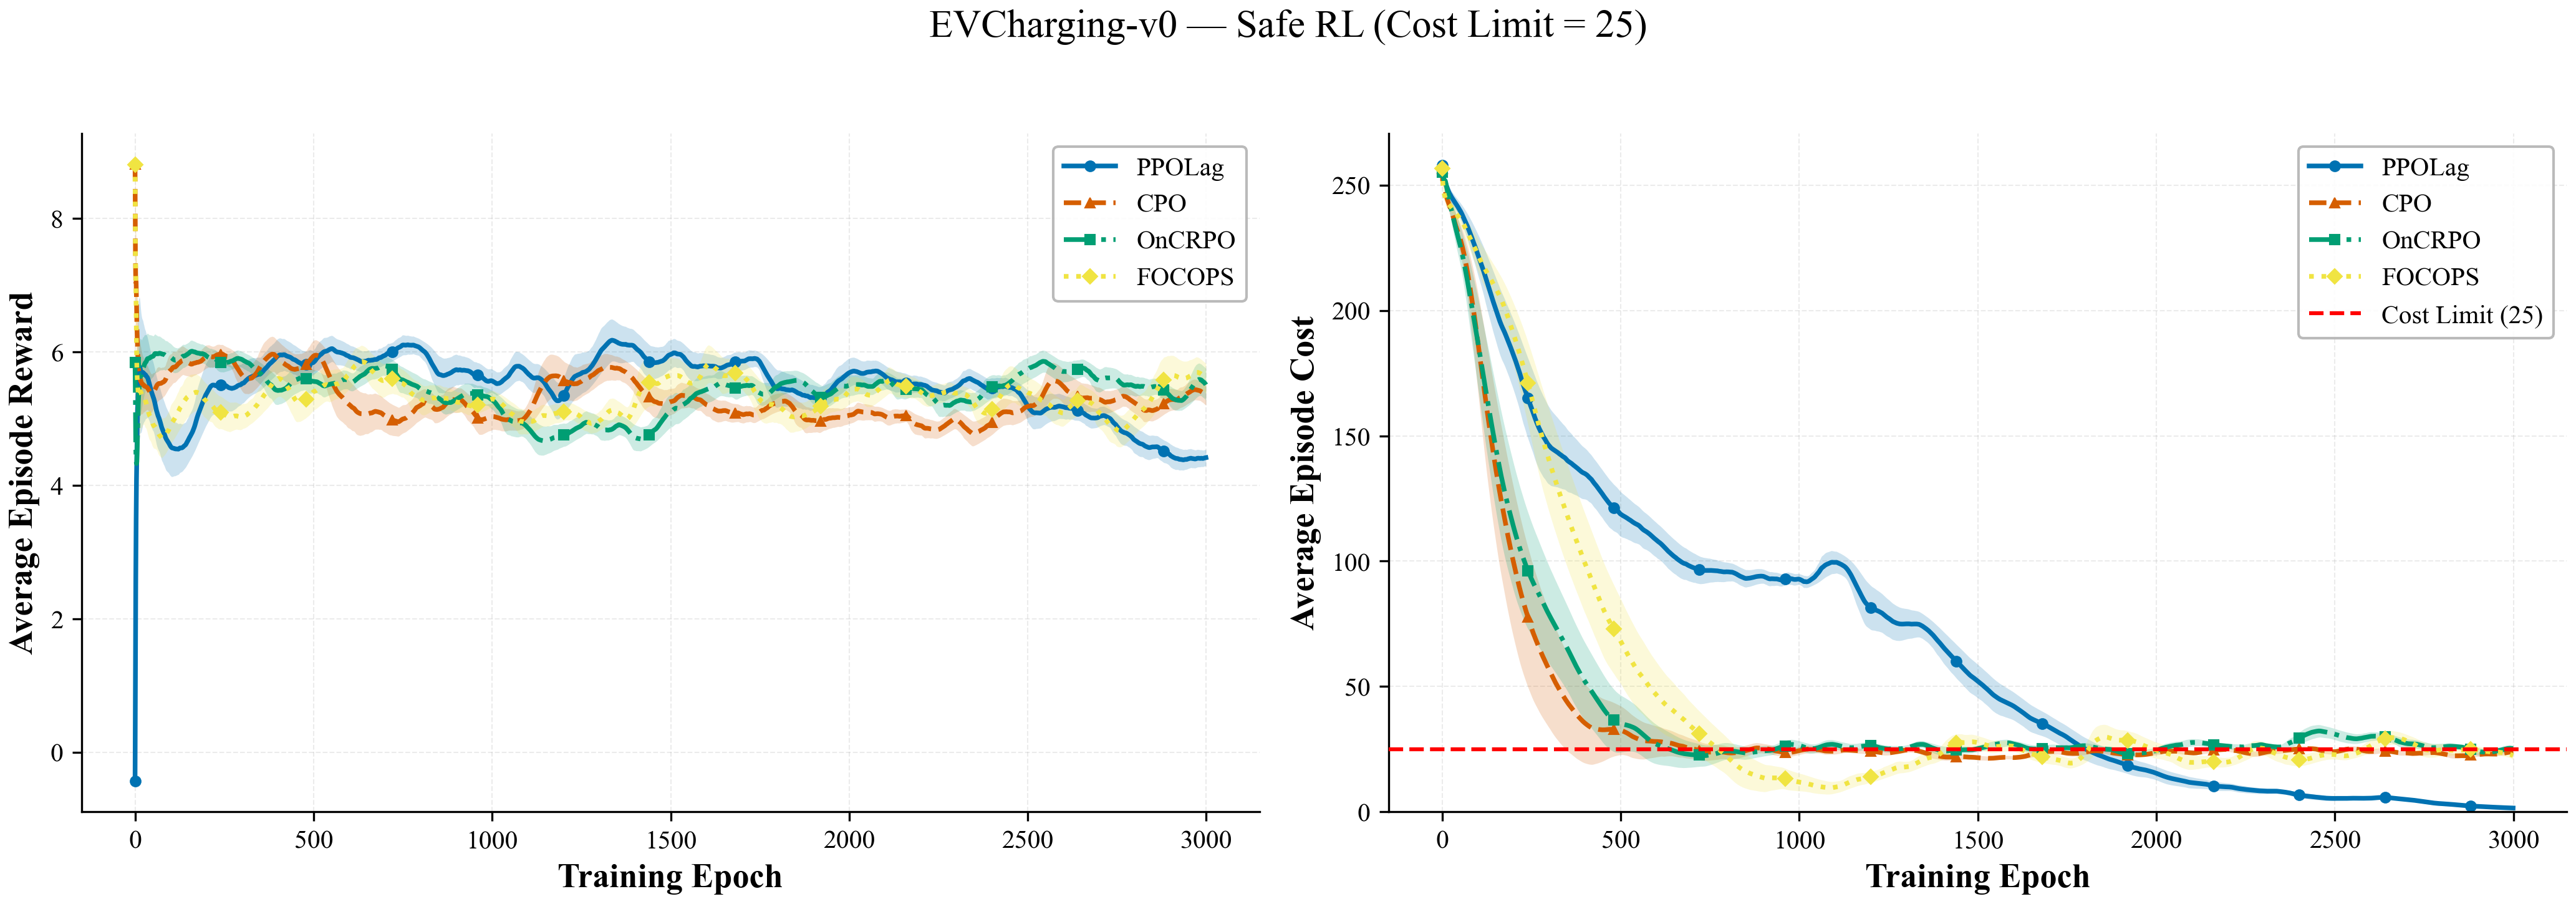
\includegraphics[width=0.9\textwidth]{figures/C_SRL/evcharging/saferl_evcharging_compare_CL25_3000ep_200ema.png}
\caption{EV Charging cross-algorithm comparison at moderate limit $d = 25$.}
\label{fig:srl_ev_cmp25}
\end{figure}

% ------------------------------------------------------------
\subsection{Building: A Negative Finding}
\label{sec:saferl_building}

Despite testing three cost function designs---raw temperature error, HVAC ramping, and deadband temperature violation---we were unable to achieve meaningful cost limit differentiation in the Building environment. \Cref{tab:building_saferl} summarizes the results.

\begin{table}[htbp]
\centering
\caption{Building Safe RL: PPOLag final episode cost across cost function designs. All limits converge to similar costs.}
\label{tab:building_saferl}
\begin{tabular}{@{}lcccc@{}}
\toprule
\textbf{Cost Function} & \textbf{$d_1$} & \textbf{$d_2$} & \textbf{$d_3$} & \textbf{$d_4$} \\
\midrule
Raw temp error & $6.7$ & $15.4$ & $12.4$ & $8.4$ \\
HVAC ramping & $6.5$ & $6.8$ & $7.2$ & $8.8$ \\
Deadband ($\delta = 1$\textdegree C) & $2.1$ & $2.3$ & $1.8$ & $2.5$ \\
\bottomrule
\end{tabular}
\end{table}

The root cause is a \emph{reward--cost alignment problem}: the reward function with $\beta = 0.5$ already strongly incentivizes both energy efficiency and thermal comfort. The agent minimizes temperature errors through reward optimization alone, trivially satisfying any temperature-based CMDP constraint.

% --- Building PPOLag ---
\subsubsection{Building --- PPOLag}

All four cost limits produce nearly identical training curves (\Cref{fig:building_ppolag}), with episode cost collapsing to $\approx 2$--$5$ regardless of the prescribed limit.

\begin{figure}[htbp]
\centering
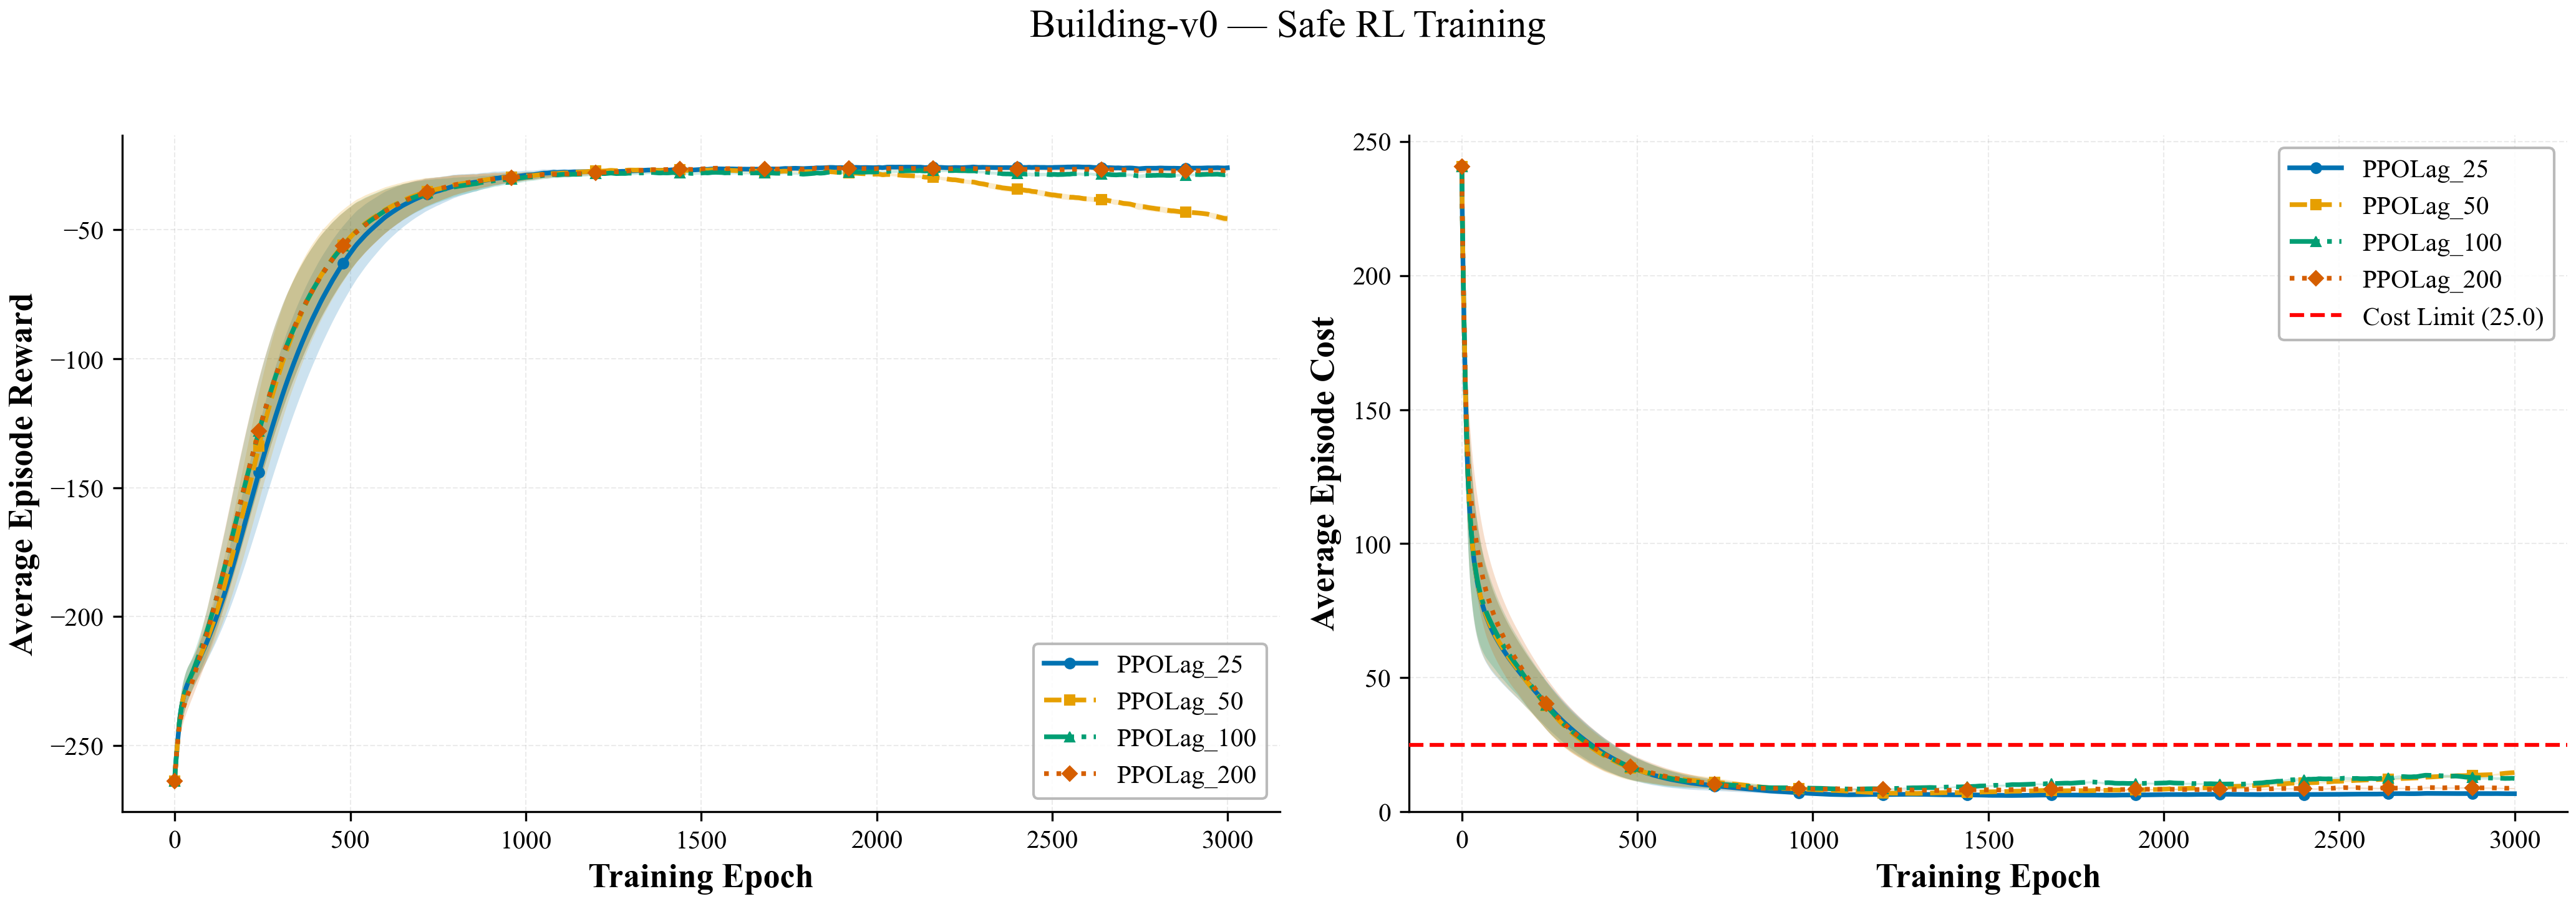
\includegraphics[width=0.9\textwidth]{figures/C_SRL/building/saferl_building_PPOLag_3000ep_200ema.png}
\caption{Building PPOLag: All four cost limits produce nearly identical training curves, demonstrating the absence of constraint differentiation.}
\label{fig:building_ppolag}
\end{figure}

% --- Building CPO ---
\subsubsection{Building --- CPO}

CPO exhibits divergence at loose limits ($d = 200, 500$), while tight limits lack differentiation (\Cref{fig:srl_bu_cpo}). This confirms the trust-region instability under nearly inactive constraints.

\begin{figure}[htbp]
\centering
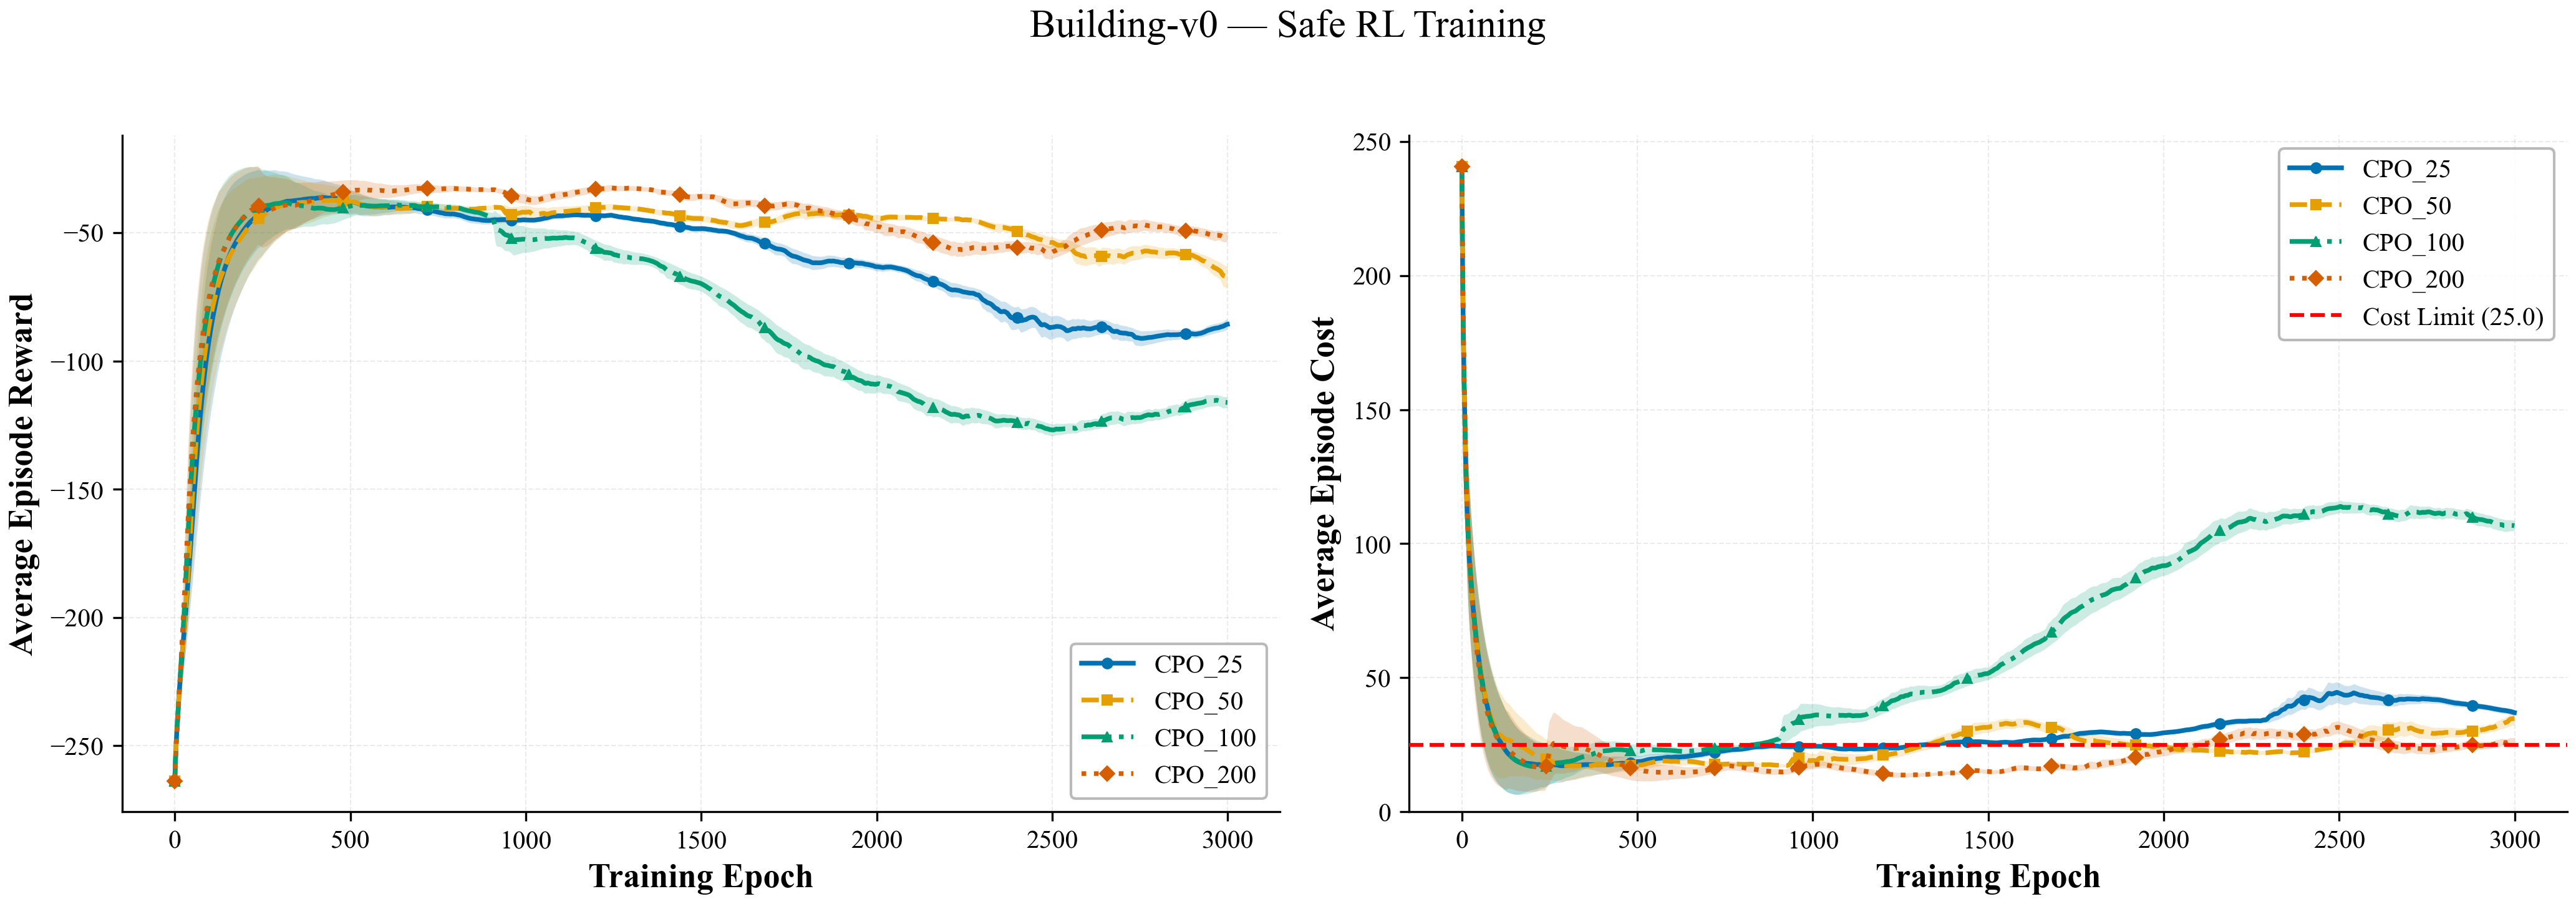
\includegraphics[width=0.9\textwidth]{figures/C_SRL/building/saferl_building_CPO_3000ep_200ema.png}
\caption{Building CPO: Loose limits ($d = 200, 500$) diverge; tight limits lack differentiation.}
\label{fig:srl_bu_cpo}
\end{figure}

% --- Building OnCRPO ---
\subsubsection{Building --- OnCRPO}

OnCRPO shows a similar divergence pattern to CPO at loose limits (\Cref{fig:srl_bu_oncrpo}), further confirming that trust-region CMDP methods are unstable when constraints are nearly inactive.

\begin{figure}[htbp]
\centering
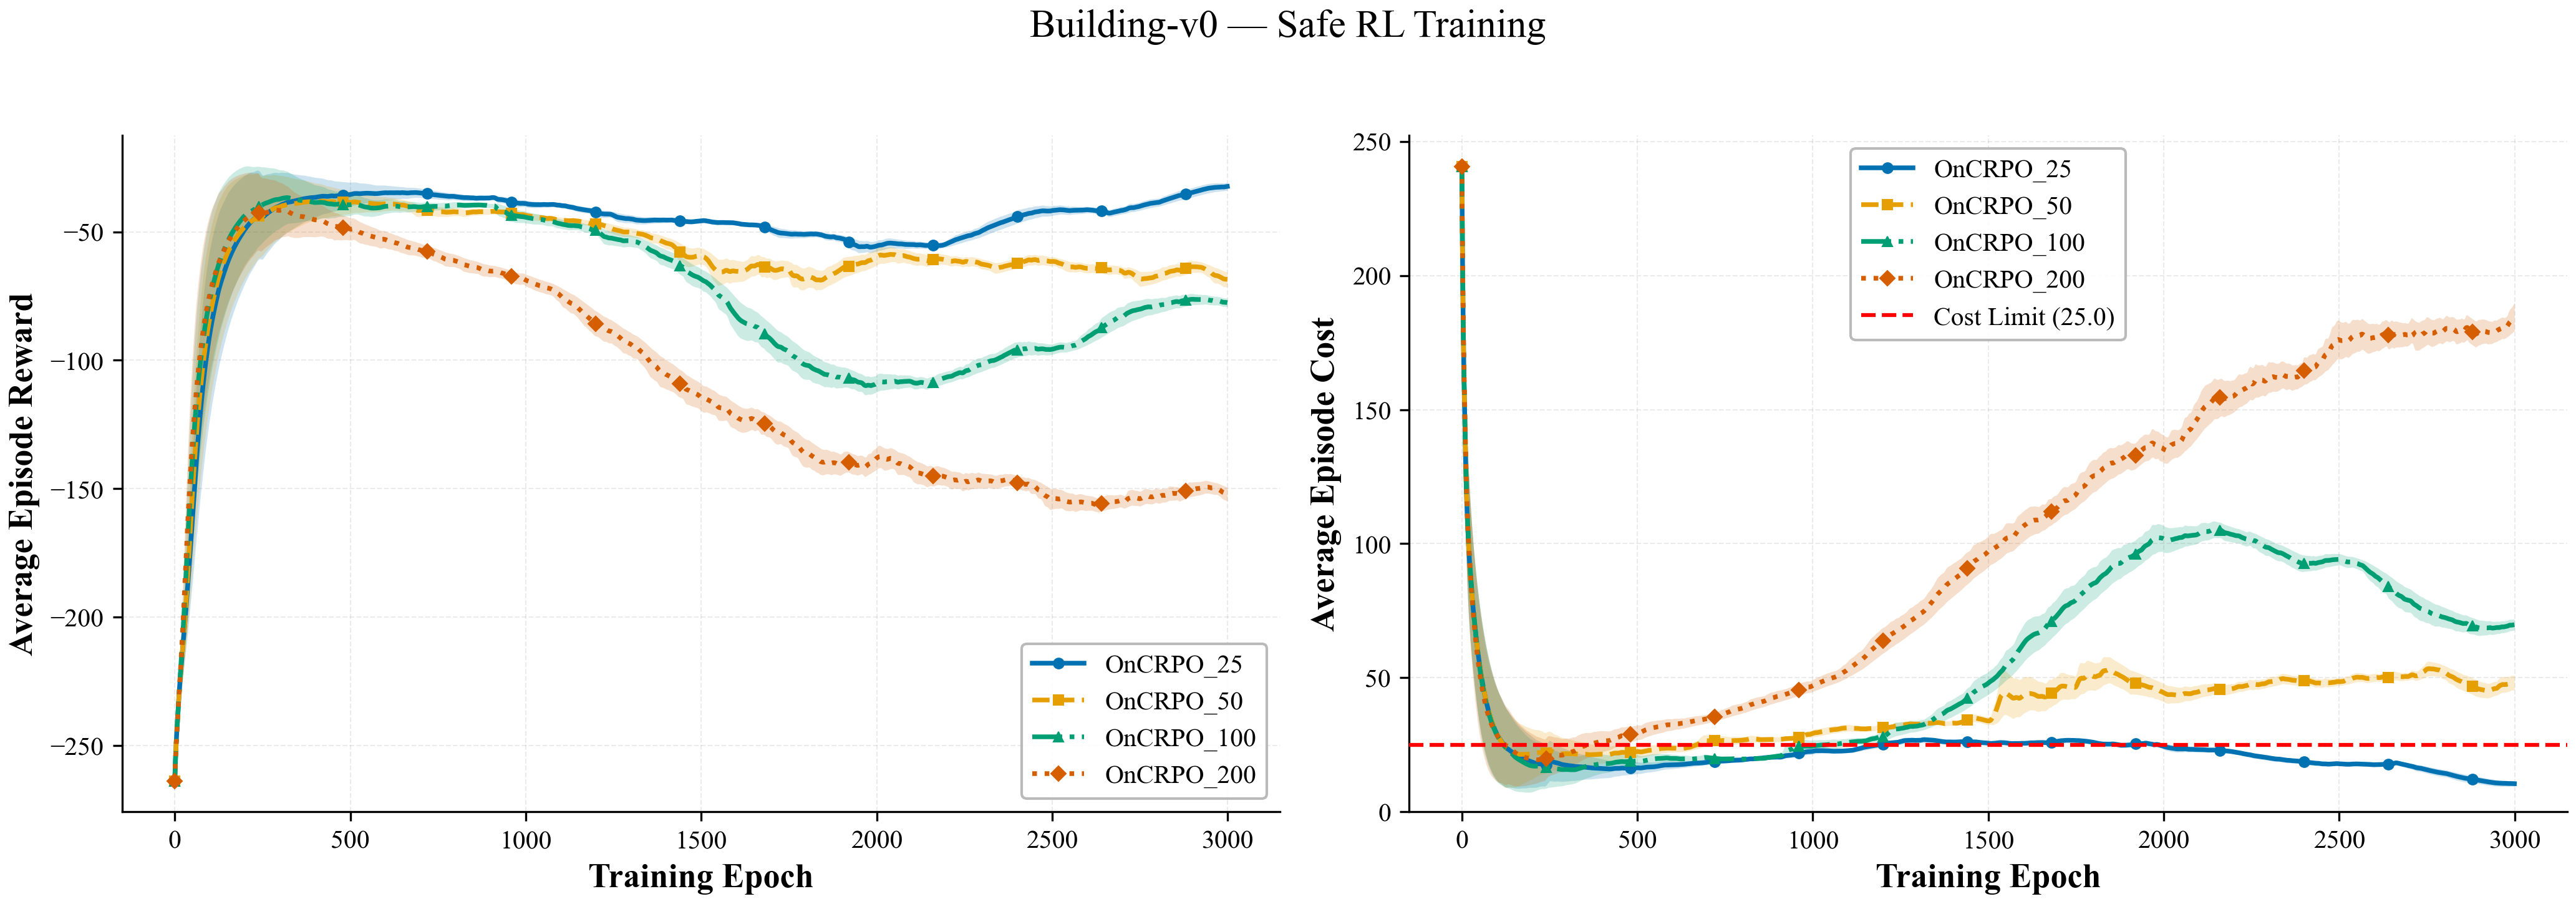
\includegraphics[width=0.9\textwidth]{figures/C_SRL/building/saferl_building_OnCRPO_3000ep_200ema.png}
\caption{Building OnCRPO: Similar divergence pattern to CPO at loose limits.}
\label{fig:srl_bu_oncrpo}
\end{figure}

% --- Building FOCOPS ---
\subsubsection{Building --- FOCOPS}

FOCOPS exhibits late-training cost increases at loose limits (\Cref{fig:srl_bu_focops}), indicating Lagrangian multiplier oscillation when the constraint is trivially satisfied.

\begin{figure}[htbp]
\centering
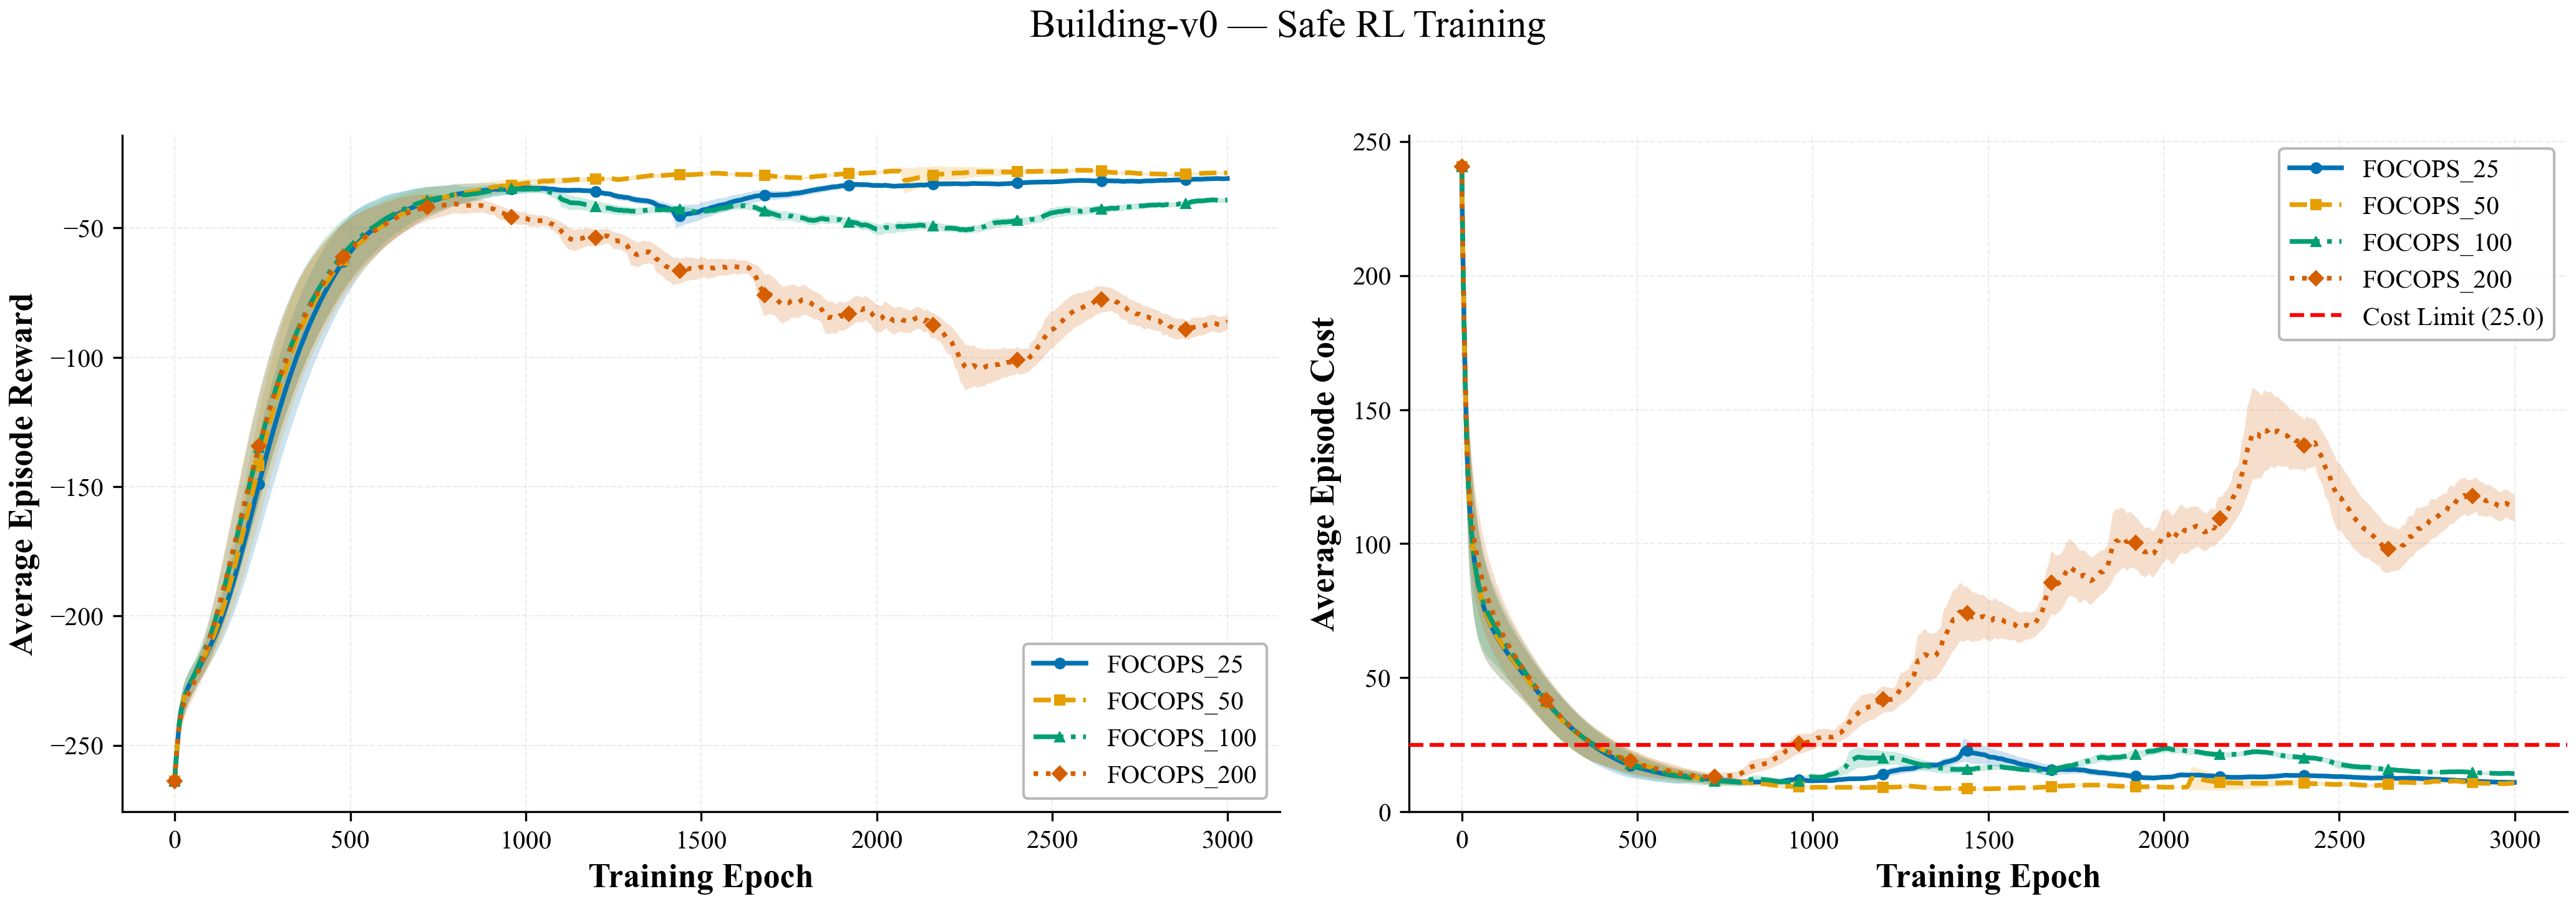
\includegraphics[width=0.9\textwidth]{figures/C_SRL/building/saferl_building_FOCOPS_3000ep_200ema.png}
\caption{Building FOCOPS: Late-training cost increase at loose limits indicates Lagrangian oscillation.}
\label{fig:srl_bu_focops}
\end{figure}

% ------------------------------------------------------------
\subsection{Off-Policy Safe RL: SACLag Failure}
\label{sec:saclag}

SACLag (SAC with Lagrangian relaxation) failed consistently across all three environments. The root cause is a fundamental incompatibility between replay buffer data staleness and Lagrange multiplier updates: the cost critic is trained on stale transitions, causing $\lambda$ to oscillate or diverge.

% ------------------------------------------------------------
\subsection{Safe RL Findings}

\begin{finding}[Reward--Cost Orthogonality Is Necessary (RQ4)]
\label{find:orthogonality}
CMDP formulations require the cost signal to measure an objective not adequately incentivized by the reward. When reward and cost are aligned (Building: $\beta = 0.5$ comfort term), constraints are trivially satisfied. When orthogonal (Cogen: ramp stress; EV: excess charge), CMDP enables precise safety--performance tradeoff control.
\end{finding}

\begin{finding}[PPOLag Is the Most Robust CMDP Algorithm (RQ4)]
\label{find:ppolag_best}
Across all environments, PPOLag provides the best cost limit differentiation, precise constraint tracking, and graceful degradation under inactive constraints ($\lambda \to 0 \Rightarrow$ standard PPO). Trust-region methods (CPO, OnCRPO) converge faster but are vulnerable to numerical instability under loose constraints.
\end{finding}

\begin{finding}[Off-Policy CMDP Methods Fail (RQ4)]
\label{find:saclag}
SACLag's replay buffer staleness prevents accurate Lagrange multiplier tracking. This negative finding suggests that on-policy methods are currently the only reliable approach for CMDP-based Safe RL.
\end{finding}

\begin{table}[htbp]
\centering
\caption{Summary of Safe RL effectiveness across environments.}
\label{tab:saferl_summary}
\begin{tabular}{@{}lcccc@{}}
\toprule
\textbf{Environment} & \textbf{Cost Signal} & \textbf{Orthogonal?} & \textbf{Differentiates?} & \textbf{Best Algo} \\
\midrule
Cogeneration & Turbine ramping & Yes & Yes & PPOLag \\
EV Charging & Excess charge & Yes & Yes (tight) & PPOLag \\
Building & Temp violation & No & No & N/A \\
\bottomrule
\end{tabular}
\end{table}

% ============================================================
\section{Multi-Agent Reinforcement Learning}
\label{sec:results_marl}

Multi-agent RL experiments are currently in progress using Ray RLlib with PettingZoo parallel environments. Preliminary results will be presented upon completion of the MARL training runs across all three environments (EVCharging: 54 agents, Building: AC-enabled zones, Cogen: 4 turbine agents).

% ============================================================
\section{Cross-Axis Discussion}
\label{sec:results_discussion}

The results across noise robustness and Safe RL reveal several cross-cutting insights.

\subsection{Environment Characteristics Matter More Than Algorithm Choice}

The most consistent finding across both experimental axes is that environment structure---not algorithm hyperparameters---determines the effectiveness of robustness and safety interventions:

\begin{itemize}
    \item \textbf{EV Charging} is inherently robust to noise (aggregate daily patterns are noise-resistant) and amenable to Safe RL (excess charge is orthogonal to profit).
    \item \textbf{Building} is inherently fragile to noise (thermal dynamics amplify errors) and resistant to Safe RL (reward already captures both objectives).
    \item \textbf{Cogeneration} shows algorithm-dependent noise sensitivity (PPO robust, SAC fragile) and strong Safe RL behavior (ramp stress is under-penalized in reward).
\end{itemize}

\subsection{PPO's Dual Advantage}

PPO emerges as the most robust algorithm across both axes: it tolerates noise better than SAC/TD3 (\Cref{sec:noise_ev,sec:noise_bu,sec:noise_co}) and provides the best CMDP constraint satisfaction as PPOLag (\Cref{sec:results_saferl}). This dual advantage stems from PPO's on-policy nature: conservative policy updates prevent both noise amplification and stale-data problems that plague off-policy methods.

\subsection{Implications for Sustainable Energy Systems}

The practical implications for real-world deployment are:

\begin{enumerate}
    \item \textbf{Sensor investment}: Observation noise is far more damaging than action noise, prioritizing sensor accuracy over actuator precision.
    \item \textbf{Safety constraint design}: CMDP constraints must measure genuinely under-optimized objectives; redundant constraints (already captured by reward) provide no benefit.
    \item \textbf{Algorithm selection}: PPO/PPOLag provides the best robustness--safety combination, despite SAC's superior clean-condition performance in some environments.
\end{enumerate}

% ============================================================
% Chapter 6: Conclusion and Future Work
% ============================================================
\chapter{Conclusion and Future Work}
\label{ch:conclusion}

This chapter summarizes the key findings of the thesis (\Cref{sec:summary}), discusses limitations (\Cref{sec:limitations}), and outlines directions for future research (\Cref{sec:future_work}).

% ============================================================
\section{Summary of Contributions and Findings}
\label{sec:summary}

This thesis presented SustainRL-Bench, a comprehensive benchmarking framework for evaluating reinforcement learning algorithms across three sustainable energy environments---electric vehicle charging coordination, building HVAC control, and cogeneration plant dispatch---along three experimental axes: perturbation robustness, safety constraints, and multi-agent coordination. We summarize the principal findings below, organized by research question.

\subsection{Perturbation Robustness (RQ1, RQ2, RQ5)}

The systematic evaluation of PPO, SAC, and TD3 under state, action, and dynamics perturbation across ten or more perturbation levels per environment yielded three key insights:

\begin{enumerate}
    \item \textbf{Environment structure dominates perturbation sensitivity.} EV Charging policies are exceptionally robust to all perturbation types ($<1\%$ degradation at moderate perturbation levels), owing to the reward's dependence on aggregate daily charging patterns rather than instantaneous observations. In contrast, Building policies degrade rapidly ($>100\%$ degradation at $\sigma \geq 0.15$) because the RC thermal model amplifies per-timestep errors through coupled zone dynamics. Cogeneration exhibits algorithm-dependent sensitivity, with PPO virtually immune and SAC degrading catastrophically under state perturbation.

    \item \textbf{State perturbation is far more damaging than action perturbation.} Across all three environments and all algorithms, state perturbation causes significantly greater performance degradation than action perturbation at equivalent scales. This finding has a clear practical implication: for real-world deployment of RL-based energy controllers, investment in sensor accuracy yields greater returns than investment in actuator precision.

    \item \textbf{PPO is the most perturbation-robust algorithm.} PPO consistently outperforms SAC and TD3 in perturbation robustness, with the most dramatic advantage in Cogeneration (PPO: $<0.3\%$ degradation; SAC: $>2000\%$). PPO's on-policy updates and clipped surrogate objective produce naturally conservative policies that tolerate input perturbations, whereas SAC's entropy-maximizing exploration can amplify perturbation through the policy output.
\end{enumerate}

\subsection{Safe Reinforcement Learning (RQ3)}

The formulation of each environment as a Constrained MDP with environment-specific cost signals revealed both successes and fundamental limitations:

\begin{enumerate}
    \item \textbf{Reward--cost orthogonality is necessary for effective CMDP constraints.} When the cost signal measures an objective already well-optimized by the reward (as in Building, where the reward's comfort term with $\beta = 0.5$ already minimizes temperature error), all cost limits produce identical behavior. In contrast, when the cost is genuinely orthogonal to the reward (Cogeneration: turbine ramping stress; EV Charging: excess charge violations), CMDP algorithms achieve precise constraint tracking with clear monotonic differentiation across cost limits.

    \item \textbf{PPOLag provides the most reliable constraint satisfaction.} Across all environments, PPOLag achieves the best cost limit differentiation and precise constraint tracking. Its Lagrangian relaxation degrades gracefully under inactive constraints ($\lambda \to 0$ reduces to standard PPO), unlike trust-region methods (CPO, OnCRPO) that can become numerically unstable when constraints are nearly satisfied.

    \item \textbf{Off-policy CMDP methods fail.} SACLag consistently failed to satisfy constraints across all three environments due to fundamental incompatibility between replay buffer staleness and Lagrange multiplier updates. This negative finding demonstrates that on-policy methods are currently necessary for reliable CMDP-based safe RL in these domains.
\end{enumerate}

\subsection{Multi-Agent Reinforcement Learning (RQ4)}

We designed and implemented multi-agent versions of all three environments using the PettingZoo parallel interface with physically motivated agent decompositions: per-station agents in EV Charging (54 agents), per-zone agents in Building HVAC, and per-turbine agents in Cogeneration (4 agents). Training with Ray RLlib using PPO, SAC, APPO, and IMPALA is ongoing; preliminary results and the complete single-agent versus multi-agent comparison will be reported in the final version of this thesis.

\subsection{Cross-Environment Insights (RQ5)}

The most consistent cross-cutting finding is that \emph{environment structure matters more than algorithm choice}: the physical characteristics of each energy system---reward aggregation timescale, dynamics coupling, and reward--cost alignment---determine the effectiveness of perturbation robustness and safety interventions more than the choice of RL algorithm or hyperparameters. This suggests that practitioners should invest primarily in understanding their specific energy system's characteristics before selecting algorithms or robustness strategies.

% ============================================================
\section{Limitations}
\label{sec:limitations}

We acknowledge the following limitations of the present work:

\begin{enumerate}
    \item \textbf{Single-seed training for perturbation experiments.} While evaluation uses 100 episodes per configuration with bootstrap confidence intervals, each perturbation-level configuration was trained with a single seed due to computational constraints. Future work should extend to multiple training seeds to capture inter-seed variability in the learned policies themselves.

    \item \textbf{Simulation-only evaluation.} All experiments are conducted in simulation environments. While SustainGym environments are grounded in real-world data and physics-based models, the sim-to-real transfer gap remains unquantified. Real-world deployment would introduce additional challenges such as non-stationary dynamics, hardware failures, and communication delays.

    \item \textbf{Building Safe RL negative result.} The Building environment's reward--cost alignment prevents meaningful CMDP constraint differentiation with the tested cost functions. While we report this as a principled negative finding (illustrating the orthogonality requirement), it means that one of the three environments does not benefit from the Safe RL axis. Alternative cost formulations---such as peak power consumption or zone-specific comfort constraints---may yield better results.

    \item \textbf{Limited MARL algorithm coverage.} The MARL experiments use independent learning with parameter sharing rather than more sophisticated CTDE algorithms such as QMIX or MADDPG. While independent learning provides a strong baseline, the comparison does not capture the full potential of cooperative MARL methods.

    \item \textbf{Fixed environment configurations.} Each environment uses a single configuration (e.g., OfficeSmall/Hot\_Dry for Building, Caltech site for EV Charging). Generalization across building types, weather profiles, or charging network topologies is not evaluated.

    \item \textbf{No combined perturbation evaluation.} Perturbation channels are evaluated independently. Real-world systems experience simultaneous state, action, and dynamics perturbation, and the interaction effects between channels may be non-additive.
\end{enumerate}

% ============================================================
\section{Future Work}
\label{sec:future_work}

Several promising directions emerge from the findings and limitations of this thesis:

\subsection{Perturbation-Aware Training and Curriculum Learning}

Our results show that policies trained under clean conditions can degrade severely under deployment perturbation (particularly in Building). A natural extension is \emph{curriculum-based perturbation training}, where the perturbation level is gradually increased during training to produce policies that are robust without sacrificing clean-condition performance. Domain randomization across perturbation levels and adversarial perturbation training~\citep{pinto2017rarl} are complementary approaches worth investigating in the energy domain.

\subsection{Cross-Environment Transfer Learning}

The three SustainGym environments share structural similarities (episodic 24-hour horizons, multi-component control, energy-comfort/cost tradeoffs) that may enable transfer learning. Pre-training on one environment and fine-tuning on another could reduce sample complexity, particularly for the data-hungry Building and Cogeneration environments. The shared perturbation injection framework provides a natural basis for evaluating whether perturbation robustness transfers across environments.

\subsection{Improved Safe RL Formulations}

The Building Safe RL negative result motivates exploration of alternative cost formulations that are genuinely orthogonal to the reward. Promising candidates include:
\begin{itemize}
    \item \textbf{Peak power constraints}: limiting the maximum instantaneous HVAC power draw, which is orthogonal to the time-averaged energy penalty in the reward.
    \item \textbf{Zone-specific comfort bounds}: enforcing hard temperature limits on individual zones rather than penalizing average deviation.
    \item \textbf{Multi-constraint CMDPs}: simultaneously constraining multiple cost signals (e.g., both energy and comfort in Building, both ramping and emissions in Cogeneration).
\end{itemize}

Additionally, the SACLag failure motivates research into off-policy CMDP methods that address replay buffer staleness, such as importance-weighted Lagrangian updates or cost-conditioned replay buffers.

\subsection{Robustness of Constrained RL Under Perturbation}

A critical open question is whether CMDP-based safety guarantees remain valid under the realistic perturbation conditions evaluated in \Cref{ch:robustness}. This thesis evaluates perturbation robustness and safe RL as independent axes; however, real-world energy systems will experience both simultaneously---a building HVAC controller must satisfy comfort constraints \emph{while} operating with noisy temperature sensors, and a cogeneration dispatcher must limit turbine ramping stress \emph{despite} uncertain ambient measurements.

Recent work by \citet{gu2025robustgymnasium} demonstrates that this concern is well-founded. Their Robust-Gymnasium benchmark evaluates safe RL algorithms (PCRPO and CRPO) on SafetyWalker2d under action perturbation and cost signal perturbation, finding that CRPO's constraint satisfaction degrades rapidly under both perturbation types, while PCRPO exhibits greater resilience---and in some cases, perturbation during training actually \emph{improves} deployment performance through a regularization effect. However, their evaluation is limited to two algorithms, a single locomotion environment, and a single cost limit, leaving the interaction between perturbation robustness and constraint satisfaction largely unexplored in applied domains.

Our SustainRL-Bench infrastructure is uniquely positioned to investigate this interaction comprehensively. The three independent perturbation channels (state, action, and dynamics) and four CMDP algorithms (PPOLag, CPO, OnCRPO, FOCOPS) are already implemented and validated independently; combining them requires no additional environment engineering. Several specific research questions arise:

\begin{itemize}
    \item \textbf{Constraint violation under perturbation}: Do policies trained with strict cost limits (e.g., $c_{\text{limit}} = 1$ for EV Charging) maintain constraint satisfaction when deployed under state perturbation? The Lagrange multiplier in PPOLag is calibrated to the training distribution; distribution shift from perturbation may cause the learned $\lambda$ to under- or over-correct.

    \item \textbf{Perturbation-aware CMDP training}: Training CMDP algorithms under perturbation simultaneously could yield policies that satisfy safety constraints robustly. This would combine the curriculum-based perturbation training discussed in \Cref{sec:future_work} with constrained optimization, effectively solving a \emph{robust} CMDP.

    \item \textbf{Environment-dependent interaction effects}: Our robustness results show that EV Charging is naturally perturbation-tolerant while Building is highly sensitive. This asymmetry likely extends to the safe RL setting: Building's tight thermal coupling may cause perturbation to amplify cost violations, while EV Charging's reward aggregation may buffer constraint satisfaction against moderate perturbation.

    \item \textbf{Cost signal corruption}: Following \citet{gu2025robustgymnasium}'s cost signal attack, perturbation applied directly to the observed cost (rather than to states or actions) tests a fundamentally different failure mode---the agent receives incorrect safety feedback, potentially learning to violate constraints while believing they are satisfied.
\end{itemize}

This direction represents a natural intersection of the perturbation robustness and safe RL axes developed in this thesis, and would provide actionable guidance for deploying constrained RL controllers in real-world energy systems where both safety and robustness are non-negotiable requirements.

\subsection{Scalable Multi-Agent Methods}

The EV Charging environment with 54 agents provides a challenging testbed for scalable MARL. Future work should investigate:
\begin{itemize}
    \item \textbf{Communication-constrained MARL}: where agents can only exchange limited information with neighbors, reflecting realistic communication constraints in charging networks.
    \item \textbf{Heterogeneous agents}: different agent types with asymmetric capabilities (e.g., fast-charging vs.\ standard stations).
    \item \textbf{Safe MARL}: combining CMDP constraints with multi-agent coordination, where safety constraints apply to the collective system behavior.
\end{itemize}

\subsection{Real-World Deployment Considerations}

Bridging the sim-to-real gap for energy RL requires addressing several practical challenges:
\begin{itemize}
    \item \textbf{Online adaptation}: policies that can adapt to non-stationary dynamics (seasonal weather changes, evolving occupancy patterns, equipment degradation) without full retraining.
    \item \textbf{Safety during exploration}: deploying RL agents in physical energy systems requires exploration strategies that never violate hard safety constraints, even during the initial learning phase.
    \item \textbf{Interpretability}: energy system operators require understanding of \emph{why} an RL agent makes specific decisions, motivating research into interpretable RL policies for energy applications.
\end{itemize}

\subsection{Extended Benchmark Coverage}

The SustainRL-Bench framework can be extended along several dimensions:
\begin{itemize}
    \item \textbf{Additional environments}: incorporating SustainGym's electricity market and data center cooling environments.
    \item \textbf{Additional algorithms}: evaluating model-based RL methods (e.g., Dreamer, MBPO) that may offer improved sample efficiency and perturbation robustness through learned dynamics models.
    \item \textbf{Combined perturbation evaluation}: systematically evaluating all combinations of state, action, and dynamics perturbation to characterize interaction effects.
    \item \textbf{Longer horizons}: extending the evaluation to multi-day or seasonal horizons to capture long-term dynamics and distribution shift.
\end{itemize}

% ============================================================
\section{Closing Remarks}
\label{sec:closing}

This thesis demonstrates that reinforcement learning holds significant promise for sustainable energy system control, but that principled evaluation across perturbation, safety, and multi-agent dimensions is essential for understanding the practical deployment landscape. The SustainRL-Bench framework, associated environments, and experimental infrastructure provide a foundation for the research community to systematically evaluate and improve RL algorithms for real-world energy applications. We hope that the findings, negative results, and open questions presented in this work will guide future research toward more robust, safe, and scalable RL-based energy controllers.


% ---- Bibliography ----
\bibliographystyle{plainnat}
\bibliography{references}

\end{document}
